\documentclass{book}
\usepackage[utf8]{inputenc}

% For multiline comments.
\usepackage{verbatim}

% For math and logic symbols
\usepackage{amsmath,amssymb,textcomp,amsthm}

% For sequent/deduction layouts.
\usepackage{bussproofs}

% Number equations by chapter/section.
\numberwithin{equation}{chapter}

% Aliases
\newcommand{\vocab}{\textbf}
\newcommand{\blank}{\underline{\hspace{1cm}}}

% Diagrams
\usepackage{tikz}
\usetikzlibrary{positioning,arrows,calc}
\tikzset{
modal/.style={>=stealth',shorten >=1pt, shorten <=1pt},
world/.style={circle,draw},
point/.style={circle,draw,inner sep=0.5mm,fill=black}
}

% Definitions, Theorems, etc.
\newtheorem{axiom}{Axiom}
\newtheorem{definition}{Definition}
\newtheorem*{anon-definition}{Definition}
\newtheorem{notation}{Notation}
\newtheorem{feature}{Feature}
\newtheorem{theorem}{Theorem}
\newtheorem*{anon-theorem}{Theorem}
\newtheorem{lemma}{Lemma}
\newtheorem*{anon-lemma}{Lemma}
\newtheorem{remark}{Remark}
\newtheorem*{anon-remark}{Remark}

% Type Derivations
\newenvironment{typederivation}
  {\begin{tabular}[t]{l l l}}
  {\end{tabular}}
\newcommand{\tdcontext}[2]
  {
    &
    \multicolumn{2}{l}{
    \begin{tabular}[t]{| l l l}
    \multicolumn{3}{| l}{#1} \\\cline{1-2}
    & & \\
    #2
    \end{tabular}
    } \\ & \\
  }
\newcommand{\tdnum}[1]{#1}
\newcommand{\tdjudge}[1]{& #1}
\newcommand{\tdjustify}[1]{& #1 \\}


\begin{document}

\title{Type Theory Handbook}
\author{JT Paasch}

\frontmatter

\maketitle


\tableofcontents


\mainmatter


%-------------------------------------------------------------------------------------------
%-------------------------------------------------------------------------------------------
%-------------------------------------------------------------------------------------------
%-------------------------------------------------------------------------------------------
\chapter{Computation}

The main question we want to ask is this: what is a computation? I think we could also use the word ``calculation'' to ask the same thing: what is a calculation? 

There are different answers to this question. We will focus on one of them. It is based on the lambda calculus and type theory. Later, we will examine the lambda calculus and type theory in detail.

But to begin, in this chapter let's think about what a ``computation'' is in an informal may, so that we have a rough idea of how the lambda calculus conceives of a computation.


%-------------------------------------------------------------------------------------------
%-------------------------------------------------------------------------------------------
\section{Solving an Arithmetic Equation}

Think about how you would solve a simple arithmetic equation, using pencil and paper. For instance, take this equation:

\begin{equation}
(1 + 2) * (3 + (1 * 2))
\end{equation}

\noindent
In our minds, we can break this up into parts, each of which we can solve separately: 

\begin{center}
\begin{tikzpicture}[]

  \node[] (p1) [] {$(1 + 2)$};
  \node[] (p2) [right=of p1] {$*$};
  \node[] (p3) [right=of p2] {$(3$};
  \node[] (p4) [right=of p3] {$+$};
  \node[] (p5) [right=of p4] {$(1 * 2))$};

\end{tikzpicture}
\end{center}

\noindent
First, we might replace $(1 * 2)$ with $2$:

\begin{center}
\begin{tikzpicture}[]

  \node[] (p1) [] {$(1 + 2)$};
  \node[] (p2) [right=of p1] {$*$};
  \node[] (p3) [right=of p2] {$(3$};
  \node[] (p4) [right=of p3] {$+$};
  \node[] (p5) [right=of p4] {$(1 * 2))$};
  
  \node[] (p6) [below=of p1] {$(1 + 2)$};
  \node[] (p7) [below=of p2] {$*$};
  \node[] (p8) [below=of p3] {$(3$};
  \node[] (p9) [below=of p4] {$+$};
  \node[] (p10) [below=of p5] {$2)$};

  \path[->] (p5) edge (p10);

\end{tikzpicture}
\end{center}

\noindent
Then we might replace $(1 + 2)$ with $3$:

\begin{center}
\begin{tikzpicture}[]

  \node[] (p1) [] {$(1 + 2)$};
  \node[] (p2) [right=of p1] {$*$};
  \node[] (p3) [right=of p2] {$(3$};
  \node[] (p4) [right=of p3] {$+$};
  \node[] (p5) [right=of p4] {$2)$};
  
  \node[] (p6) [below=of p1] {$3$};
  \node[] (p7) [below=of p2] {$*$};
  \node[] (p8) [below=of p3] {$(3$};
  \node[] (p9) [below=of p4] {$+$};
  \node[] (p10) [below=of p5] {$2)$};

  \path[->] (p1) edge (p6);

\end{tikzpicture}
\end{center}


\noindent
Then we would replace $(3 + 2)$ with $5$:

\begin{center}
\begin{tikzpicture}[]

  \node[] (p1) [] {$3$};
  \node[] (p2) [right=of p1] {$*$};
  \node[] (p3) [right=of p2] {$(3$};
  \node[] (p4) [right=of p3] {$+$};
  \node[] (p5) [right=of p4] {$2)$};
  
  \node[] (p6) [below=of p1] {$3$};
  \node[] (p7) [below=of p2] {$*$};
  \node[] (p8) [below=of p4] {$5$};
  
  \path[->] (p4) edge (p8);

\end{tikzpicture}
\end{center}

\noindent
And finally, we would replace $3 * 5$ with $15$:

\begin{center}
\begin{tikzpicture}[]

  \node[] (p1) [] {$3$};
  \node[] (p2) [right=of p1] {$*$};
  \node[] (p3) [right=of p2] {$5$};
  
  \node[] (p4) [below=of p2] {$15$};
  
  \path[->] (p2) edge (p4);

\end{tikzpicture}
\end{center}

\noindent
What can we observe about this process? Here are some points to notice:

\begin{itemize}
\item{The whole equation is made up of many parts.}
\item{Some parts can be replaced by other parts (e.g., $(1 + 2)$ can be replaced with $3$).}
\item{We can perform such replacements multiple times.}
\item{Sometimes, new replacements become possible after we perform another replacement (e.g., after we replace $(1 * 2)$ with $2$, we then get $(3 + 2)$, which wasn't there before, and it can be replaced too).}
\item{The process terminates. That is, there is a point where we cannot replace any more parts of the equation.}
\end{itemize}

\noindent
This is an example of computation or calculation. We compute the answer by successively replacing parts of the equation with other parts, until we cannot make any more replacements.


%-------------------------------------------------------------------------------------------
%-------------------------------------------------------------------------------------------
\section{Calculation by Rewriting}

Let us look at this same process in a slightly different way. Let us think about this process not as a process of solving parts of an equation, but rather as a process of rewriting. 

To do that, think of the equation as nothing more than a string of characters: it is just a sequence of symbols (what they mean is irrelevant). We can break this string up into smaller chunks (subsequences). For instance, take the subsequence $(1 * 2)$:

\begin{center}
$(1 + 2) * (3 + \underline{(1 *2)})$
\end{center}

\noindent
We can replace that subsequence with a new subsequence, namely $2$:\footnote{$2$ is a sequence that contains only one symbol. In some situations, we might also replace a subsequence with an empty subsequence, i.e., a blank sequence with no symbols at all.}

\begin{center}
$(1 + 2) * (3 + \underline{2})$
\end{center}

\noindent
Then we can take the subsequence $(3 + 2)$ and replace it with a new subsequence: $5$.

\begin{center}
$(1 + 2) * \underline{5}$
\end{center}

\noindent
We can then take the subsequence $(1 + 2)$ and replace it with $3$:

\begin{center}
$\underline{3} * 5$
\end{center}

\noindent
And finally, we can replace the sequence $3 * 5$ with $15$:

\begin{center}
$15$
\end{center}

\noindent
This time around, we are talking about sequences and subsequences of symbols, rather than parts of an equation. Still, we can observe the same properties as before:

\begin{itemize}
\item{The whole sequence of symbols is made up of many subsequences.}
\item{Some subsequences can be replaced by other subsequences (e.g., $(1 + 2)$ can be replaced with $3$).}
\item{We can perform such replacements multiple times.}
\item{Sometimes, new replacements become possible after we perform another replacement (e.g., after we replace $(1 * 2)$ with $2$, we then get $(3 + 2)$, which wasn't there before, and it can be replaced too).}
\item{The process terminates. That is, there is a point where we cannot replace any more subsequences.}
\end{itemize}

\noindent
Notice that we don't have to know that the above sequence of symbols is an equation. The symbols we used could have been any symbols at all, but we could still walk through the same process of taking certain subsequences and replacing them with other sequences.


%-------------------------------------------------------------------------------------------
%-------------------------------------------------------------------------------------------
\section{String Replacment}

Let's pursue the above line of thought with an even more radical example. Suppose we have an arbitrary string of characters:

\begin{center}
\texttt{ebceeb}
\end{center}

\noindent
We could, in principle, do some kind of replacement/reduction on this too. For instance, we could say that we want to take every \texttt{e}:

\begin{center}
\texttt{\underline{e}bc\underline{ee}b}
\end{center}

\noindent
And then replace each one with a zero:

\begin{center}
\texttt{\underline{0}bc\underline{00}b}
\end{center}

\noindent
Next, we could take every \texttt{b}:

\begin{center}
\texttt{0\underline{b}c00\underline{b}}
\end{center}

\noindent
And replace each one with nothing (an empty sequence):

\begin{center}
\texttt{0c00}
\end{center}

\noindent
Finally, we might take every subsequence of \texttt{0c}:

\begin{center}
\texttt{\underline{0c}00}
\end{center}

\noindent
And replace it with a one:

\begin{center}
\texttt{\underline{1}00}
\end{center}

\noindent
This would be a kind of reduction or rewrite process too, in just the same sense as before:

\begin{itemize}
\item{The whole sequence of symbols is made up of many subsequences.}
    \item{Some subsequences can be replaced by other subsequences (e.g., \texttt{e} can be replaced with \texttt{0}).}
\item{We can perform such replacements multiple times.}
\item{Sometimes, new replacements become possible after we perform other replacements (e.g., after we replace \texttt{e} with \texttt{0} and \texttt{b} with nothing, we then get \texttt{0c}, which wasn't there before, and it can be replaced too).}
\item{The process terminates. That is, there is a point where we cannot replace any more subsequences.}
\end{itemize}

\noindent
So this too counts as a computation or calculation in just the way that the other examples did. But this example is more radical because there is no obvious meaning to the symbols. In this case, we are doing nothing but mindless symbol manipulation, of the sort that a computer does.


%-------------------------------------------------------------------------------------------
%-------------------------------------------------------------------------------------------
\section{The Basic Operations of Rewriting}

In every one of the above examples, we performed three basic operations. Here they are:

\begin{itemize}
\item{Identify a sequence of symbols to replace: in each case above, we said something like this: ``the sequence $xyz$ can be replaced.''}
\item{Stipulate what to replace it with: in each case we said something like this: ``replace the replaceable sequence with $abc$.''}
\item{Do the actual replacement: in each case, we then took the sequence to replace, we deleted it, and we replaced it with the stipulated replacement.}
\end{itemize}

\noindent
Think of this at the most basic level. By ``basic,'' I mean: imagine that we can only replace one symbol at a time, so that complex replacements are accomplished by stringing together multiple one-symbol replacements. The operations are still the same:

\begin{itemize}
\item{Identify a symbol to replace.}
\item{Stipulate a replacement.}
\item{Do the replacement.}
\end{itemize}

\noindent
From these three basic operations, we can perform any of the computations or calculations that we did above. In fact, we can model pretty much any computation at all with these three simple operations.


%-------------------------------------------------------------------------------------------
%-------------------------------------------------------------------------------------------
\section{Computation Generally}

At a very general level, we have here a process where we replace symbols with other symbols, and this is independent of whatever the meaning of those symbols might be.

This is the basic idea behind a ``calculation'' or ``computation,'' as we will conceive of it here. A \vocab{computation} is a finite set of replacements on a sequence of symbols.

The \vocab{lambda calculus} is an attempt to formalize this process of calculation. In certain ways, it is very simple. Nevertheless, with the lambda calculus we can build up a remarkable number of things. 

Later, we will add types to the lambda calculus, which will restrict its generality, but will give us some very useful power and precision.


%-------------------------------------------------------------------------------------------
%-------------------------------------------------------------------------------------------
%-------------------------------------------------------------------------------------------
%-------------------------------------------------------------------------------------------
\chapter{The Lambda Calculus (Informally)}

There are three basic operations in the lambda calculus: abstraction, application, and $\beta$-reduction. These correspond to the three basic operations of rewriting that we mentioned in the last chapter. Abstraction is when you identify a symbol to replace, application is when you stipulate a replacement, and $\beta$-reduction is when you do the replacement.


%-------------------------------------------------------------------------------------------
%-------------------------------------------------------------------------------------------
\section{Abstraction}

Suppose I need to repeat some trivial calculation a lot. For instance, suppose that each day this week I need to buy $2$ pounds of sand, at $5$ cents per pound. I'm a forgetful person, so I write it down:

\begin{equation}
\text{multiply 2 by 5}
\end{equation}

\noindent
Suppose that next week, the price goes up to $7$ cents per pound, so I cross out my note and write down:

\begin{equation}
\text{multiply 2 by 7}
\end{equation}

\noindent
The third week it is $4$ cents per pound:

\begin{equation}
\text{multiply 2 by 4}
\end{equation}

\noindent
After a while, I wise up and realize I can make a formula out of this. To do that, I can use a name instead of a number for the price:

\begin{equation}
\text{multiply 2 by \underline{price}}
\end{equation}

\noindent
Then I can indicate up front that I intend for the word ``price'' to be replaced:

\begin{equation}
\text{replace ``price'' in (multiply 2 by price)}
\end{equation}

\noindent
In lamba calculus terminology, this is called an \vocab{abstraction}. We say we \vocab{abstract} ``price'' from the body of the original expression. What we have done here is identified the symbol (or in this case, word) that is replaceable in the original expression.


%-------------------------------------------------------------------------------------------
%-------------------------------------------------------------------------------------------
\section{Application}

Next, we can stipulate what value should be used to replace ``price.'' For instance, to calculate the cost if the sand is $5$ cents per pound:

\begin{equation}
\text{replace ``price'' with ``$5$'' in (multiply 2 by price)}
\end{equation}

\noindent
We could substitute another value in for ``price'' too. For instance, the price could be $7$:

\begin{equation}
\text{replace ``price'' with ``$7$'' in (multiply 2 by price)}
\end{equation}

\noindent
In lambda calculus terminology, this is called an \vocab{application}. We say that we \vocab{apply} the expression to $7$ (or to $5$ in the previous case). What we have done here is stipulated what the replacement is.

Note: the term ``application'' can be misleading. We do not actually apply anything here. All we do with an ``application'' is we stipulate the value that should be used to replace ``price''; but we do not do any replacing here.


%-------------------------------------------------------------------------------------------
%-------------------------------------------------------------------------------------------
\section{Beta Reduction}

Consider the above application:

\begin{equation}
\text{replace ``price'' with ``$5$'' in (multiply 2 by price)}
\end{equation}

\noindent
We can do the actual replacement --- we can put ``$5$'' in the place of ``price'' --- to get this:

\begin{equation}
\text{multiply 2 by 5}
\end{equation}

\noindent
Or we can put ``$7$'' in the place of ``price,'' which comes out to this:

\begin{equation}
\text{multiply 2 by 7}
\end{equation}

\noindent
In lambda calculus terminology, when we replace the names with stipulated replacements in the body of the expression, we call this a \vocab{$\beta$-reduction} (or just ``beta reduction'' if you don't want to write the Greek character).


%-------------------------------------------------------------------------------------------
%-------------------------------------------------------------------------------------------
\section{Nesting Abstractions and Applications}

You can nest abstractions and applications. Take the abstraction we made above:

\begin{equation}
\text{replace ``price'' in (multiply 2 by price)}
\end{equation}

\noindent
We can abstract the weight too:

\begin{equation}
\text{replace ``weight'' in (replace ``price'' in (multiply weight by price))}
\end{equation}

\noindent
Notice how the one abstraction is nested inside the other. We can nest applications too. Let us stipulate that we want to replace ``weight'' with ``$3$'':

\begin{equation}
\text{replace ``weight'' with ``3'' in (replace ``price'' in (multiply weight by price))}
\end{equation}

\noindent
When we enact the $\beta$-reduction (i.e., when we put ``$3$'' in place of ``weight''), we get this:

\begin{equation}
\text{replace ``price'' in (multiply 3 by price)}
\end{equation}

\noindent
We can then stipulate that we want to replace ``price'' with ``$7$'':

\begin{equation}
\text{replace ``price'' with ``7'' in (multiply 3 by price)}
\end{equation}

\noindent
And once we actually do the $\beta$-reduction, we get:

\begin{equation}
\text{multiply 3 by 7}
\end{equation}


%-------------------------------------------------------------------------------------------
%-------------------------------------------------------------------------------------------
%-------------------------------------------------------------------------------------------
%-------------------------------------------------------------------------------------------
\chapter{Replacements (Informally)}


%-------------------------------------------------------------------------------------------
%-------------------------------------------------------------------------------------------
\section{Free and Bound Names}

When you formulate an abstraction, you identify a name that is replaceable. Once you identify a name as a name that can be replaced, we say that the name is \vocab{bound} by the abstraction. 

In the informal formulation we have been using so far, we know a name is bound when we see the phrase ``replace [name] in'' up front. That tells us that ``[name]'' is bound. For example, consider our earlier abstraction:

\begin{equation}
\text{replace ``price'' in (multiply 2 by price)}
\end{equation}

\noindent
Here we have bound the word ``price.'' The phrase

\begin{equation}
\text{replace ``price'' in (\ldots)}
\end{equation}

\noindent
is called a \vocab{binding expression}.

Anything in the expression that is not bound is called \vocab{free}. So, the words ``multiply,'' ``2,'' and ``by'' are all free. The only word that is bound in the above abstraction is ``price.''

Suppose we take away the abstraction, and look at the original expression by itself:

\begin{equation}
\text{multiply 2 by price}
\end{equation}

\noindent
What about ``price'' now? Is it bound here? No, it is not. And we know that because there is no binding expression up front that says ``replace price in.'' So, by itself, ``price'' is free in the original expression. But when it appears in the abstraction --- i.e., 

\begin{equation}
\text{replace ``price'' in (multiply 2 by price)}
\end{equation}

\noindent
--- then the word ``price'' is not free. Rather, it is bound.


%-------------------------------------------------------------------------------------------
%-------------------------------------------------------------------------------------------
\section{Capturing Names}

When you nest abstractions, parent abstractions can bind names that were free in a child expression. We say that the parent abstraction \vocab{captures} the free name from the child. 

Consider this abstraction:

\begin{equation}
\text{replace ``price'' in (multiply weight by price)}
\end{equation}

\noindent
Here the word ``price'' is bound by the binding expression. But the word ``weight'' is not bound. It is free.

Now suppose we nest this whole abstraction inside another abstraction, one that binds the word ``weight'':

\begin{equation}
\text{replace ``weight'' in (replace ``price'' in (multiply weight by price))}
\end{equation}

\noindent
Now the word ``weight'' is bound, by the outermost binding expression. That word was free before, but here it gets bound. We say that the parent binding expression captured it, and bound it.


%-------------------------------------------------------------------------------------------
%-------------------------------------------------------------------------------------------
\section{Not Just Any Replacement}

In a $\beta$-reduction, you replace a bound name with another value. If you are not careful though, you can unintentionally bind a name that isn't supposed to be bound. 

Consider again this nested abstraction:

\begin{equation}
\text{replace ``weight'' in (replace ``price'' in (multiply weight by price))}
\end{equation}

\noindent
What happens if we stipulate that we want to replace the bound ``weight'' with the word ``price''? Like this:

\begin{equation}
\text{replace ``weight'' with ``price'' in (replace ``price'' in (multiply weight by price))}
\end{equation}

\noindent
When we do the $\beta$-reduction, we get this:

\begin{equation}
\text{replace ``price'' in (multiply price by price)}
\end{equation}

\noindent
Here, we have replaced the free word ``weight'' with the word ``price.'' But ``price'' is bound in this expression, so now we have unintentionally bound a part of the expression that wasn't bound before.

For this reason, in the lambda calculus, you can't use any replacements that are \vocab{already bound} in the expression. In our example here, the word ``price'' is a forbidden replacement, since it is already bound in the expression.





%-------------------------------------------------------------------------------------------
%-------------------------------------------------------------------------------------------
%-------------------------------------------------------------------------------------------
%-------------------------------------------------------------------------------------------
\chapter{Equivalence (Informally)}


%-------------------------------------------------------------------------------------------
%-------------------------------------------------------------------------------------------
\section{$\alpha$-conversion}

Consider our earlier abstraction:

\begin{equation}
\text{replace ``price'' in (multiply 2 by price)}
\end{equation}

\noindent
We could replace the word ``price'' with something else. For instance:

\begin{equation}
\text{replace ``$x$'' in (multiply 2 by $x$)}
\end{equation}

\noindent
We could even replace ``price'' with some random word:

\begin{equation}
\text{replace ``bargle'' in (multiply 2 by bargle)}
\end{equation}

\noindent
When we rename the bound names in an expression like this, it is called an \vocab{$\alpha$-conversion}. For instance, replacing ``price'' with ``$x$'' as we did above is an $\alpha$-conversion. 

We say that these terms are \vocab{$\alpha$-variants} of each other. For instance, the ``price'' version and the ``$x$'' version are $\alpha$-variants.


%-------------------------------------------------------------------------------------------
%-------------------------------------------------------------------------------------------
\section{Computational Equivalence}

$\alpha$-variants are equivalent, in the sense that when you do a $\beta$-reduction, you get the same result. Take our earlier abstraction:

\begin{equation}
\text{replace ``price'' in (multiply 2 by price)}
\end{equation}

\noindent
Replace the bound name with $5$:

\begin{equation}
\text{replace ``price'' with ``5'' in (multiply 2 by price)}
\end{equation}

\noindent
Do the $\beta$-reduction, and you get:

\begin{equation}
\text{multiply 2 by 5}
\end{equation}

\noindent
Now take the expression where we used $x$ as the bound name, and do the same:

\begin{align}
\text{replace ``$x$'' in (multiply 2 by $x$)} \\
\text{replace ``$x$'' with ``5'' in (multiply 2 by $x$)} \\
\text{multiply 2 by 5}
\end{align}

\noindent
Finally, try it with the ``bargle'' variant:

\begin{align}
\text{replace ``bargle'' in (multiply 2 by bargle)} \\
\text{replace ``bargle'' with ``5'' in (multiply 2 by bargle)} \\
\text{multiply 2 by 5}
\end{align}

\noindent
In each case, the very same computation happens. The name we give to the bound name does not matter, because it is always replaced in the same way.

Another way to say this is that these $\alpha$-variants can be \vocab{substituted} for each other. They \vocab{preserve} the same computation.


%-------------------------------------------------------------------------------------------
%-------------------------------------------------------------------------------------------
\section{The Class of Equivalent Terms}

Each of the above $\alpha$-variants are equivalent. We can collect them together, and say, ``these are all equivalent.'' 

We can add many other expressions to the class. Just put in a new bound name --- change ``price'' to ``$y$,'' ``$\circ$,'' ``\textbf{M},'' ``slapf,'' or whatever --- and you have a new $\alpha$-variant.

So, there is a bundle of variations that are all basically the same term, through $\alpha$-equivalence. Mathematicians sometimes use the word ``modulo'' instead of ``through'': these terms are equivalent \vocab{modulo $\alpha$-equivalence}.

The crucial thing to note is that the same $\beta$-reductions apply to any variant in the class. Whatever you can compute with one variant, you can compute with the other variants.

In practice, writers often just pick a binding name, e.g., ``$x$,'' and then talk about that selected $\alpha$-variant as \textit{the} expression. But really, they mean it as a representative; there is a large collection of other variants which could be substituted in at any time. 


%-------------------------------------------------------------------------------------------
%-------------------------------------------------------------------------------------------
%-------------------------------------------------------------------------------------------
%-------------------------------------------------------------------------------------------
\chapter{$\lambda$ Variables}

The untyped lambda calculus is a formal way of doing everything that we stalked about informally earlier. Instead of writing ``untyped lambda calculus,'' I will say $\lambda$.

Let us first establish the notation --- i.e., how you actually write expressions down. $\lambda$ expressions are built up from what are called \vocab{terms}. Let us start with the simplest type of $\lambda$ term. These are called variables.


%-------------------------------------------------------------------------------------------
%-------------------------------------------------------------------------------------------
\section{Variables}

Earlier, we used English words (and sometimes symbols like $x$) to build expressions. But formally, we do not need to use actual words. We only need symbols.

So, let us say that our alphabet is a collection of symbols that we can pick from. Let us say we can pick any lowercase letter:

\begin{equation}
a, b, c, \ldots, v, x, y, z
\end{equation}

\noindent
If we need to, we can attach subscripted numbers to make more. For instance:

\begin{equation}
v_{1}, v_{2} \ldots, x_{1}, x_{2}, \ldots x_{56}, x_{57}, \ldots
\end{equation}

\noindent
In $\lambda$, these are called \vocab{variables}. Be careful here. The word ``variable'' means something different in, say, first-order logic, or in programming languages. In $\lambda$, it refers to any single symbol taken from the alphabet we specified here.

The simplest expression you can build in $\lambda$ consists of a single variable. To construct such an expression, select a variable from the alphabet and wrap it in parentheses. For instance:

\begin{equation}
(x)
\end{equation}

\noindent
The following are all valid $\lambda$ variable terms:

\begin{align}
(y) \\
(a) \\
(v_{9})
\end{align}


%-------------------------------------------------------------------------------------------
\subsection{Dropping Parentheses}

We wrap terms in parentheses in order to avoid ambiguity. One of the things that parentheses do is tell us where a term begins and where it ends.

Another thing that parentheses do is tell us how symbols should be grouped together. In a moment, we will see cases where this is important. 

But for a single variable, there is no grouping. Hence, when the term is a single variable term, there is no confusion if you omit the parentheses. For instance, this:

\begin{equation}
(x)
\end{equation}

\noindent
can easily be written like this:

\begin{equation}
x
\end{equation}

\noindent
and nobody will be confused about it.

In practice, most writers omit parentheses around a single-variable term, and we will too. 

However, this is just a typographical convenience. If anyone demands that we write down the term in the fully correct way, we should always be able to put the parentheses back.


%-------------------------------------------------------------------------------------------
%-------------------------------------------------------------------------------------------
%-------------------------------------------------------------------------------------------
%-------------------------------------------------------------------------------------------
\chapter{Abstractions}

Earlier, we talked about abstractions. Abstractions occur when you select a name (or symbol) from an expression, and stipulate that it can be replaced. Our example was this:

\begin{equation}
\text{replace ``price'' in (multiply 2 by price)}
\end{equation}

\noindent
We can put this more generally. Let us use the symbol $\phi$ to stand in the place of \textit{whatever} word or symbol we want to mark as replaceable (e.g., ``price''), and let us use the symbol $M$ to stand in place of \textit{whatever} expression we want to make the replacements in (e.g., ``multiply 2 by price''). Then we can write it like this:

\begin{equation}
\text{replace $\phi$ in ($M$)}
\end{equation}

\noindent
In $\lambda$, we can write this more compactly. The notation looks like this:

\begin{equation}
\lambda \phi . (M)
\end{equation}

\noindent
The lower case Greek $\lambda$ (lambda) character indicates ``replace,'' and in fact this is where the lambda calculus gets its name. 

Be careful when you see this $\lambda$ character. Sometimes I use it to refer to the whole system that we call the untyped lambda calculus. But other times, I use it as part of an abstraction term. The context should always make it clear which I mean.


%-------------------------------------------------------------------------------------------
%-------------------------------------------------------------------------------------------
\section{Forming the Terms}

To construct an \vocab{abstraction}, you take any term, and you mark a variable value as replaceable. For instance, take this term, which consists of a single variable:

\begin{equation}
(x)
\end{equation}

\noindent
Let us suppose that we want to make $x$ replaceable. To mark the value $x$ as replaceable, put $\lambda x$ up front, followed by a dot:

\begin{equation}
\lambda x.(x)
\end{equation}

\noindent
finally wrap the whole thing in parentheses:

\begin{equation}
(\lambda x.(x))
\end{equation}

\noindent
That says:

\begin{equation}
\text{Replace ``$x$'' in ($x$)}
\end{equation}

\noindent
Here is some terminology:

\begin{itemize}

\item{``$\lambda x.$'' is called the \vocab{binding expression}.}

\item{The ``$x$'' in ``$\lambda x.$'' is called the \vocab{binding variable}.}

\item{Everything after the binding expression is called the \vocab{body} of the abstraction.}

\end{itemize}

\noindent
Here is a diagram of all these parts, labeled:

\begin{center}
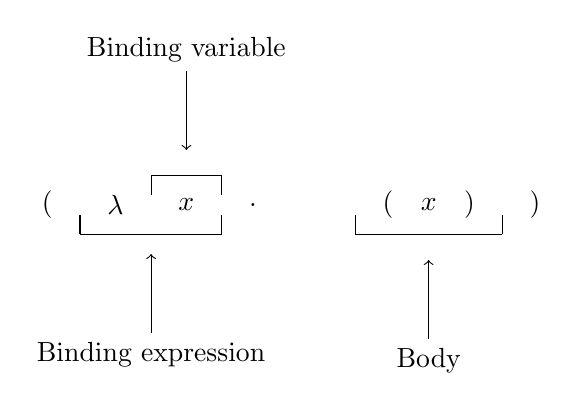
\begin{tikzpicture}[]

  \node[] (p0) [] {(};
  \node[] (p1) [right=.1cm of p0] {};
  \node[] (p2) [right=.1cm of p1] {$\lambda$};
  \node[] (p3) [right=.1cm of p2] {};
  \node[] (p4) [right=.1cm of p3] {$x$};
  \node[] (p5) [right=.1cm of p4] {};
  \node[] (p6) [right=.1cm of p5] {.};
  \node[] (p7) [right=of p6] {};
  \node[] (p8) [right=.1cm of p7] {(};
  \node[] (p9) [right=.1cm of p8] {$x$};
  \node[] (p10) [right=.1cm of p9] {)};
  \node[] (p11) [right=.1cm of p10] {};
  \node[] (p12) [right=.1cm of p11] {)};

  \node[coordinate] (a0) [above=.25cm of p3] {};
  \node[coordinate] (a1) [above=.25cm of p5] {};
  \node[] (a2) [above=.25cm of p4] {};
  \node[] (a3) [above=of a2] {Binding variable};
  
  \draw[] (p3)--(a0);
  \draw[] (p5)--(a1);
  \draw[] (a0)--(a1);
  \path[->] (a3) edge (a2);
  
  \node[coordinate] (b0) [below=.25cm of p1] {};
  \node[coordinate] (b1) [below=.25cm of p5] {};
  \node[] (b2) [below=.25cm of p3] {};
  \node[] (b3) [below=of b2] {Binding expression};

  \draw[] (p1)--(b0);
  \draw[] (p5)--(b1);
  \draw[] (b0)--(b1);
  \path[->] (b3) edge (b2);
  
  \node[coordinate] (c0) [below=.25cm of p7] {};
  \node[coordinate] (c1) [below=.25cm of p11] {};
  \node[] (c2) [below=.25cm of p9] {};
  \node[] (c3) [below=of c2] {Body};

  \draw[] (p7)--(c0);
  \draw[] (p11)--(c1);
  \draw[] (c0)--(c1);
  \path[->] (c3) edge (c2);

\end{tikzpicture}
\end{center}


%-------------------------------------------------------------------------------------------
\subsection{Nested Terms}

The body of an abstraction can be any term. In our last example, it was a single variable. But it could be a complex term, like another lambda term. For instance:

\begin{equation}
(\lambda x.(\lambda y.(x)))
\end{equation}

\noindent
We will discuss applications next, but note here that the body of an abstraction could also be an application.


%-------------------------------------------------------------------------------------------
\subsection{Dropping Parentheses}

As with variable terms, we can drop parentheses in abstractions if it leads to no ambiguity. Consider this abstraction:

\begin{equation}
(\lambda x.(x))
\end{equation}

\noindent
We can drop the outer parentheses, and the expression is still unambiguous:

\begin{equation}
\lambda x.(x)
\end{equation}

\noindent
We can also drop the parentheses around the body of the expression:

\begin{equation}
\lambda x.x
\end{equation}

\noindent
Now consider this term:

\begin{equation}
(\lambda x.(\lambda x. (x)))
\end{equation}

\noindent
We can drop the outer parentheses without losing clarity:

\begin{equation}
\lambda x.(\lambda x. (x))
\end{equation}

\noindent
We can also drop the rest of the parentheses without losing clarity:

\begin{equation}
\lambda x.\lambda x. x
\end{equation}

\noindent
In these cases, we can freely drop parentheses without losing clarity. But in a moment we will discuss applications, and there we will encounter cases where we need to include parentheses to avoid ambiguity.


%-------------------------------------------------------------------------------------------
%-------------------------------------------------------------------------------------------
%-------------------------------------------------------------------------------------------
%-------------------------------------------------------------------------------------------
\chapter{$\lambda$ Applications}

When we talked about $\lambda$ informally above, we talked about applications. An \vocab{application} occurs when you stipulate a value to put in place of a bound name. We did this by saying what the replacement should be. For example:

\begin{equation}
\text{replace ``price'' with ``5'' in (multiply 2 by price)}
\end{equation}

\noindent
Here we say that the value ``5'' should be put in place of ``price.'' We say that value ``5'' is the \vocab{argument}.

In $\lambda$, we write this slightly differently. We put the argument after the formula, something like this:

\begin{equation}
\text{replace ``price'' in (multiply 2 by price) 5}
\end{equation}

\noindent
Of course, we can represent this more generally. We can use a symbol to stand in place of the whole formula, minus the argument. Let $M$ stand for the formula. Then we can write:

\begin{equation}
M~5
\end{equation}

\noindent
We could use another symbol to stand for the argument too. Let $N$ stand for the argument. Then we can write:

\begin{equation}
M N
\end{equation}

\noindent
That is the basic notation we use in $\lambda$ to write applications.


%-------------------------------------------------------------------------------------------
%-------------------------------------------------------------------------------------------
\section{Forming the Terms}

To construct an \vocab{application} in $\lambda$, put any two terms next to each other, and wrap the whole of them in parentheses. For instance:

\begin{equation}
((\lambda x.(x)) (y))
\end{equation}

\noindent
Here the first term is $(\lambda x.(x))$ and the second term is $(y)$. We say that we \vocab{apply} the first term to the second term, and as we noted a moment ago, we say that the second term is the \vocab{argument}.

In this case, the first term is an abstraction. But in $\lambda$ this need not be so. \textit{Any} two terms can be put next together to form an application. Here we put two variable terms next to each other --- $(x)$ and $(y)$:

\begin{equation}
((x) (y))
\end{equation}

\noindent
Here are some other examples:

\begin{align}
((a) (b)) \\
((x) (\lambda x.(y))) \\
((\lambda x.((a)(b))) ((v_{1}) (v_{10})))
\end{align}


%-------------------------------------------------------------------------------------------
\subsection{Nested Applications}

Notice that I said an application consists of any two \textit{terms} next to each other. An application is itself a term. So you can make an application from other applications. For instance:

\begin{equation}
(((x) (y)) (x))
\end{equation}

\noindent
The first term of the application is $((x) (y))$ --- which is itself an application of $(x)$ to $(y)$ --- and the second term of the application is $(x)$. So we apply $((x)(y))$ to $(x)$.


%-------------------------------------------------------------------------------------------
\subsection{Dropping Parentheses}

Parentheses can be dropped if no ambiguity comes of it. Consider this:

\begin{equation}
((x) (y))
\end{equation}

\noindent
We could drop the outer parentheses, and there is no ambiguity:

\begin{equation}
(x) (y)
\end{equation}

\noindent
And we could drop the parentheses around the variables too:

\begin{equation}
x y
\end{equation}

\noindent
But now consider this:

\begin{equation}
(((x) (y)) (x))
\end{equation}

\noindent
Suppose you drop all the parentheses:

\begin{equation}
x y x
\end{equation}

\noindent
Now it is not clear what this expression means. It could be this:

\begin{equation}
(x y) x
\end{equation}

\noindent
Or this:

\begin{equation}
x (y x)
\end{equation}

\noindent
So in this case, we need at least one set of parentheses to make it unambiguous. Here is another example, with all parentheses dropped:

\begin{equation}
\lambda x.x y
\end{equation}

\noindent
This is ambiguous. It could mean this:

\begin{equation}
\lambda x.(x y)
\end{equation}

\noindent
Or it could mean this:

\begin{equation}
(\lambda x.x) y
\end{equation}

\noindent
So here too, we need at least one set of parentheses to make the expression unambiguous.

Writers often stipulate a convention so they don't have to write so many parentheses. For instance, they often say that you should always assume the parentheses group to the left. Hence, this:

\begin{equation}
x y x
\end{equation}

\noindent
means this:

\begin{equation}
(x y) x
\end{equation}

\noindent
It is always a good idea to read an author's notes about their notation, so you can be clear about their parentheses conventions.

We will not adopt a convention here. But we will drop parentheses if it results in no ambiguity. If strict correctness is demanded, we should always be able to put the parentheses back.


%-------------------------------------------------------------------------------------------
%-------------------------------------------------------------------------------------------
%-------------------------------------------------------------------------------------------
%-------------------------------------------------------------------------------------------
\chapter{Variable Occurrences}

Variables can occur in multiple places inside $\lambda$ terms. For instance, they can occur on their own, as single variable terms. They can occur in applications and in the body of abstractions. And they can occur as binding variables. It is important to keep all these types of occurrences separate.


%-------------------------------------------------------------------------------------------
%-------------------------------------------------------------------------------------------
\section{Free and Bound Variables}

In an abstraction, there is a binding variable. In the body of the abstraction, we say that every occurrence of that value is \vocab{bound} by that binding variable. Every other variable that occurs in the body is \vocab{free}. Consider this abstraction:

\begin{equation}
\lambda x.(x y)
\end{equation}

\noindent
The body of the expression is $(x y)$. The $x$ that occurs there is bound by $\lambda x$. The $y$ that occurs there is free.

Note, however, that a binding variable binds \textit{every occurrence} of a value. Consider this abstraction:

\begin{equation}
\lambda x.(x (x y))
\end{equation}

\noindent
Here the body of the abstraction is $(x (x y))$. Now we have two occurrences of $x$. Both are bound by $\lambda x$, while $y$ is still free.

A bound value does not need to occur in the body of the expression. This is a valid abstraction:

\begin{equation}
\lambda x.y
\end{equation}

\noindent
But there is no occurrence of $x$ in the body of this abstraction.


%-------------------------------------------------------------------------------------------
\subsection{Free Inside, Bound Outside}

Consider this abstraction:

\begin{equation}
\lambda x.(x y)
\end{equation}

\noindent
In this term, the body is $(xy)$, and the $x$ is bound by $\lambda x$. The $y$ is free.

Now consider the body of the abstraction all by itself, without the abstraction:

\begin{equation}
(x y)
\end{equation}

\noindent
Is $x$ bound or free? In this case, it is free, since there is no binding expression.

Writers sometimes speak in the same sentence about how variables are both bound and free. On a first read, you might think, ``how can it be bound \textit{and} free?'' 

Well, the writer simply means that a variable is free ``inside'' the body of the expression, when we consider the body of the expression all by itself, but the variable is bound from the ``outside'' by an abstracting binding expression.


%-------------------------------------------------------------------------------------------
%-------------------------------------------------------------------------------------------
\section{Multiple Occurrences of a Term}

It is important to keep the value of a variable separate from the occurrence of the variable. Consider this term again:

\begin{equation}
((x y) x)
\end{equation}

\noindent
The same variable ($x$) appears twice. Technically, we say that there are multiple \vocab{occurrences} or multiple \vocab{instances} of the same \vocab{value}. 

We could rewrite the above to be more explicit, something like this:

\begin{center}
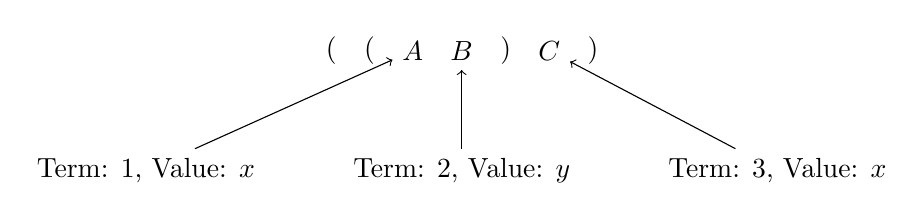
\begin{tikzpicture}[]

  \node[] (p0) [] {(};
  \node[] (p1) [right=.1cm of p0] {(};
  \node[] (p2) [right=.1cm of p1] {$A$};
  \node[] (p3) [right=.1cm of p2] {$B$};
  \node[] (p4) [right=.1cm of p3] {)};
  \node[] (p5) [right=.1cm of p4] {$C$};
  \node[] (p6) [right=.1cm of p5] {)};

  \node[] (a0) [below=of p3] {Term: 2, Value: $y$};
  \node[] (a1) [left=of a0] {Term: 1, Value: $x$};
  \node[] (a2) [right=of a0] {Term: 3, Value: $x$};
  
  \path[->] (a0) edge (p3);
  \path[->] (a1) edge (p2);
  \path[->] (a2) edge (p5);
  
\end{tikzpicture}
\end{center}

\noindent
That makes it clearer that we have three separate variable terms here, and each has their own value. The value of 1 and 3 is $x$, and the value of 2 is $y$.


%-------------------------------------------------------------------------------------------
%-------------------------------------------------------------------------------------------
%-------------------------------------------------------------------------------------------
%-------------------------------------------------------------------------------------------
\chapter{Terms}

Let us define $\lambda$ terms formally.


%-------------------------------------------------------------------------------------------
%-------------------------------------------------------------------------------------------
\section{The Format}

As we saw before, there are three types of lambda terms (parentheses are dropped where it leaves no ambiguity):

\begin{itemize}
\item{Variables --- e.g., $a$, $b$, $x$, $y$, $v_{1}$, $v_{2}$, etc.}
\item{Applications -- e.g., $xy$, $ab$, $(ab)x$, $(xx)(xy)$, etc.}
\item{Abstractions -- e.g., $\lambda x.x$, $\lambda x.(xy)$, $\lambda y.(x(ab))$, etc.}
\end{itemize}

\noindent
Applications and abstraction terms can have other terms nested inside of them. For instance, an application has this form:

\begin{equation}
MN
\end{equation}

\noindent
where $M$ and $N$ are placeholders that can stand for \textit{any} $\lambda$ terms. For instance, these are all valid applications:

\begin{itemize}
\item{$xy$ --- so $M = x$ and $N = y$.}
\item{$(xy)y$ --- so $M = (xy)$ and $N = y$.}
\item{$x(\lambda x.(ab))$ --- so $M = x$ and $N = (\lambda x.(ab))$.}
\end{itemize}

\noindent
An abstraction has this form:

\begin{equation}
\lambda \phi.M
\end{equation}

\noindent
where $\phi$ is a placeholder for any value of a variable term, and $M$ is a placeholder for any lambda term. These are all valid abstractions:

\begin{itemize}
\item{$\lambda x.(x)$ --- so $\phi = x$ and $M = (x)$.}
\item{$\lambda y.(ab)$ --- so $\phi = y$ and $M = (ab)$.}
\item{$\lambda a.((\lambda x.x)a)$ --- so $\phi = a$ and $M = ((\lambda x.x)a)$.}
\end{itemize}


%-------------------------------------------------------------------------------------------
%-------------------------------------------------------------------------------------------
\section{Definition}

With this information at hand, let us formulate a definition of lambda terms. Let us say that a lambda term is any string of characters that are built by using one of the following rules:  

\begin{itemize}
\item{Take the set of possible variables $a, b, c, \ldots$ (we call this the alphabet we can choose from), pick any one of them, and surround it with parentheses, e.g., $(a)$ or $(b)$.}
\item{Take any two terms, call them $M$ and $N$, put them next to each other, and surround them with parentheses, e.g., $(ab)$ or $((bc)a)$.}
\item{Take the value of any variable, call it $\phi$, and take any term, call it $M$, and put them together like this: $(\lambda \phi.M)$, e.g., $(\lambda a.(a))$ or $(\lambda b.(a b))$.}
\end{itemize}

\noindent
Here it is, more exactly:

\begin{definition}[The set $\Lambda$ of all lambda terms]
Let $V$ be an infinite set of symbols, possibly with subscripts: $V = {a, b, c, \ldots x, y, z, \ldots v_{1}, v_{2}, \ldots}$. Then $\Lambda$ is the set of all terms that satisfy the following conditions:

\begin{itemize}
\item{If $\phi \in V$, then $(\phi) \in \Lambda$ (call this type of term a \vocab{variable}).}
\item{If $M, N \in \Lambda$, then $(MN) \in \Lambda$ (call this type of term an \vocab{application}).}
\item{If $\phi \in V$ and $M \in \Lambda$, then $(\lambda \phi.M) \in \Lambda$ (call this type of term an \vocab{abstraction}).}
\end{itemize}
\end{definition}


%-------------------------------------------------------------------------------------------
%-------------------------------------------------------------------------------------------
\section{Explanation}

$V$ is the set of all symbols in our alphabet, and the capital Greek letter $\Lambda$ (Lambda) is the set of all $\lambda$ terms. According to this definition, all the terms in $\Lambda$ are of three types. 

\begin{itemize}

\item{First, there are variable terms, which are formed by taking a symbol $\phi$ from $V$ (in set theory notation, we write: $\phi \in V$, where $\in$ means ``in''), and putting parentheses around it, like this: $(\phi)$. Any term formed that way is in $\Lambda$. (In set theory notation: $(\phi) \in \Lambda$.)}

\item{Second, there are application terms, which are formed by taking any two terms $M$ and $N$ from $\Lambda$ (in set theory notation: $M, N \in \Lambda$), then putting them next to each other, and wrapping them in parentheses, like his: $(MN)$.}

\item{Third, there are abstraction terms, which are formed by taking the value of any symbol $\phi$ in $V$ (in set theory notation: any $\phi \in V$) and taking any term $M$ in $\Lambda$ (in set theory notation: $M \in \Lambda$), and putting them together like this: $(\lambda \phi.M)$.}

\end{itemize}

\noindent
Notice that there are an infinite number of terms in $\Lambda$: 

\begin{itemize}

\item{Variables can be formed by taking symbols out of $V$. But there are an infinite number of symbols in the alphabet $V$. So there are an infinite number of variable terms in $\Lambda$.}

\item{Applications and abstractions can be formed by taking any other terms from $\Lambda$. So, you can form terms out of terms out of terms out of terms, infinitely.}

\end{itemize}

\noindent
Of course, as we have said, we can drop parentheses when it leads to no ambiguity, but if absolute strictness is ever demanded of us, we should always be able to put the parentheses back in.


%-------------------------------------------------------------------------------------------
%-------------------------------------------------------------------------------------------
%-------------------------------------------------------------------------------------------
%-------------------------------------------------------------------------------------------
\chapter{Subterms}

Application terms and abstraction terms can be built from other $\lambda$ terms. So, terms can have subterms. Let us define subterms formally.


%-------------------------------------------------------------------------------------------
%-------------------------------------------------------------------------------------------
\section{The Terms in a Variable}

The subterms of a $\lambda$ term will include all the terms it is built from, plus itself. Consider a variable term first:

\begin{equation}
(x)
\end{equation}

\noindent
There is just one term here, namely the variable term $(x)$. So the list of subterms is this:

\begin{itemize}
\item{$(x)$}
\end{itemize}


%-------------------------------------------------------------------------------------------
%-------------------------------------------------------------------------------------------
\section{The Terms in an Application}

Consider an application term like this one:

\begin{equation}
(xx)
\end{equation}

\noindent
This is an application term, but it is composed of two variable terms: $x$ and $x$. The total list of subterms in this term are these:

\begin{itemize}
\item{$x$}
\item{$x$}
\item{$(xx)$}
\end{itemize}

\noindent
There are three subterms here. There are two occurrences of the variable $x$, and there is the larger whole, which is the application $(xx)$. We can diagram this, in a tree format:

\begin{center}
\begin{tikzpicture}[]

  \node[] (p0) [] {appl.};
  \node[] (p1) [below left= of p0] {$x$};
  \node[] (p2) [below right=of p0] {$x$};

  \path[->] (p0) edge (p1);
  \path[->] (p0) edge (p2);
  
\end{tikzpicture}
\end{center}

\noindent
You can tell how many subterms are in this term by counting the nodes in the tree. In this case, there are three nodes: the top node (the application), plus the two branches (the two variable terms).


%-------------------------------------------------------------------------------------------
%-------------------------------------------------------------------------------------------
\section{The Terms in an Abstraction}

Consider this term:

\begin{equation}
\lambda x.(xy)
\end{equation}

\noindent
This is an abstraction term, but the body of the abstraction is an application composed of two variable terms. So the total list of subterms is this:

\begin{itemize}
\item{$x$}
\item{$y$}
\item{$(xy)$}
\item{$\lambda x.(xy)$}
\end{itemize}

\noindent
We can diagram that like this:

\begin{center}
\begin{tikzpicture}[]

  \node[] (p0) [] {$\lambda x$};
  \node[] (p1) [below=of p0] {appl.};
  \node[] (p2) [below left= of p1] {$x$};
  \node[] (p3) [below right=of p1] {$y$};

  \path[->] (p0) edge (p1);
  \path[->] (p1) edge (p2);
  \path[->] (p1) edge (p3);
  
\end{tikzpicture}
\end{center}

\noindent
Again, you can determine how many subterms there are here by counting the number of nodes. There are four: the top node (the abstraction), its child (the application), plus the two branches (the two variables).


%-------------------------------------------------------------------------------------------
%-------------------------------------------------------------------------------------------
\section{Sets or Multisets?}

On a first pass, you might think we could say the subterms of a term is the \textit{set} of terms that the term is built from. However, a set cannot have any repetitions. Consider this term again:

\begin{equation}
(xx)
\end{equation}

\noindent
When we list the subterms here, we get this list:

\begin{itemize}
\item{$x$}
\item{$x$}
\item{$(x x)$}
\end{itemize}

\noindent
Now suppose we put those into a set:

\begin{equation}
\{ (x), (x), (x x) \}
\end{equation}

\noindent
Of course, repetitions don't matter in a set, so we remove the duplicate $(x)$ to get this:

\begin{equation}
\{ (x), (x x) \}
\end{equation}

\noindent
Unfortunately, that does not represent all the subterms. It's missing one!

To allow for repetitions, we need to use a multiset. A \vocab{multiset} is a set that allows multiple occurrences of the same item. (That is why a multipset is called a \textit{multi}set --- the name is short for a \textit{mult}iple membership \textit{set}.)

So, we can say that the subterms are the \textit{multiset}:

\begin{equation}
\{ (x), (x), (x x) \}
\end{equation}


%-------------------------------------------------------------------------------------------
%-------------------------------------------------------------------------------------------
\section{Definition}

With the above information in mind, let us define subterms formally. Let us say that the subterms of a term is the multiset of terms it is built from. There are three types of terms a term can be built from, so we need to enumerate each case:

\begin{itemize}
\item{If the term is a variable $(x)$, then the multiset will contain just that variable.}
\item{If the term is an application $(M N)$, then the multiset will contain all the subterms contained in $M$, and all the subterms contained in $N$, plus the application $(M N)$ itself.}
\item{If the term is an abstraction $(\lambda \phi.M)$, then the multiset will contain all the subterms contained in $M$, plus the abstraction $(\lambda \phi.M)$ itself.}
\end{itemize}

\noindent
We can unite multiple multisets into one big multiset. We call this the \vocab{union} of the multisets. The union of two multisets will include every element in each set. We write it like this: the union of multisets $A$ and $B$ is notated as $A \cup B$.

Here is our definition:

\begin{definition}[The multiset $Sub$ of subterms in a $\lambda$ term $M$]
Let $M$ be a lambda term, and let $V$ be the set of variables defined above. The multiset $Sub$ of subterms in $M$ (notated as $Sub(M)$) is the smallest multiset that satisfies the following conditions:

\begin{itemize}
\item{If $M$ is a variable $x \in V$, then $Sub(x)$ is $\{ x \}$.}
\item{If $M$ is an application of the form $M N$, then $Sub(M N)$ is the union of the multisets $Sub(M)$, $Sub(N)$, and $\{ (M N) \}$, i.e., $Sub(M) \cup Sub(N) \cup \{(M N)\}$.}
\item{If $M$ is an abstraction of the form $\lambda \phi.M$, then $Sub(\lambda \phi.M)$ is the union of the multisets $Sub(M)$ and $\{ (\lambda \phi.M) \}$, i.e., $Sub(M) \cup \{ (\lambda \phi.M) \}$.}
\end{itemize}

\end{definition}


%-------------------------------------------------------------------------------------------
%-------------------------------------------------------------------------------------------
\section{Proper Subterms}

The subterms of a term include the larger term itself. If we want to talk about just the subterms, without the larger term itself, we can call those terms the \vocab{proper subterms} of the term. We can define that like this:

\begin{definition}[Proper subterms]
Let $M$ be a lambda term. For any subterm $N \in Sub(M)$, $N$ is a proper subterm of $M$ if $N \not = M$. 
\end{definition}

\noindent
So, take any subterm in a term $M$, and that subterm is a proper subterm if it is not identical to $M$. 


%-------------------------------------------------------------------------------------------
%-------------------------------------------------------------------------------------------
%-------------------------------------------------------------------------------------------
%-------------------------------------------------------------------------------------------
\chapter{Free Variables}

The purpose of an abstraction term is to stipulate a value that can be replaced in another term. It has this form:

\begin{equation}
\lambda x.M
\end{equation}

\noindent
This is a short hand notation for this: ``replace `x' in $M$.'' An abstraction like this has three parts:

\begin{itemize}
\item{The \vocab{binding expression}, which is $\lambda x.$}
\item{The \vocab{binding variable}, which is $x$.}
\item{The \vocab{body} of the expression, which is $M$.}
\end{itemize}

\noindent
Any occurrence of $x$ inside $M$ is \vocab{bound} (by the binding expression $\lambda x$). Any other variable that occurs in $M$ is said to be \vocab{free}. Let us define bound and free variables formally.


%-------------------------------------------------------------------------------------------
%-------------------------------------------------------------------------------------------
\section{Finding all Free Variables}

The free variables in a $\lambda$ term will include every variable that is not bound. Let us refer to thihs set with the name $FV$, and we will say that the set of free variables in a term $M$ is $FV(M)$.

\begin{notation}
$FV(M)$ stands for the set of free variables $FV$ in a $\lambda$ term $M$. 
\end{notation}

\noindent
There are three different types of terms: variables, applications, and abstractions. Let us consider how we gather the free variables for each case.


%-------------------------------------------------------------------------------------------
\subsection{Variable Terms}

A variable term has this form:

\begin{equation}
(\phi)
\end{equation}

\noindent
What are the free variables in this expression? Well, it is the variable itself, $x$. And this will be true for any variable term at all. If a term is just a variable, that variable will be free. 

Let $\phi$ be a placeholder that stands for any variable. Then we can say this: take any variable term of this form:

\begin{equation}
(\phi)
\end{equation}

\noindent
The set of free variables in this expression will consist only of $\phi$:

\begin{equation}
FV(\phi) = \{ \phi \}
\end{equation}


%-------------------------------------------------------------------------------------------
\subsection{Application Terms}

An application has this form:

\begin{equation}
(x y)
\end{equation}

\noindent
What are the free variables in this expression? Well, there are two: $x$ and $y$. So the set of free variables in this case are these:

\begin{equation}
FV((x y)) = \{ x, y \}
\end{equation}

\noindent
But let's think more generally about this. An application is really just two terms, next to each other. So this is really the set of free variables in the first term, plus the set of free variables in the second term:

\begin{equation}
FV((x y)) = FV(x) \text{ plus } FV(y)
\end{equation}

\noindent
In set theory terminology, we can say that the free variables in the application are the \textit{union} of the free variables of the first term and the second term:

\begin{equation}
FV((x y)) = FV(x) \cup FV(y)
\end{equation}

\noindent
In this case, the two terms in the application are $x$ and $y$. But the same thing holds no matter the terms are. Suppose we have an application like this:

\begin{equation}
((x y) y)
\end{equation}

\noindent
Now the first term is itself an application --- $(x y)$ --- while the second term is a variable $y$. Nevertheless, the free variables in this expression will be the set of free variables in the first term, plus the set of free variables in the second term:

\begin{equation}
FV(((x y) y)) = FV((x, y)) \cup FV(y)
\end{equation}

\noindent
And of course, we could then reduce this further, and get the free variables for each of $x$ and $y$ in the innermost application:

\begin{align}
FV(((x y) y)) = \\ FV((x, y)) \cup FV(y) = \\ (FV(x) \cup FV(y)) \cup FV(y)
\end{align}

\noindent
We can keep going down into nested application like this, to figure out what the free variables are in an application.

To formulate this in a general way, let us say that $M$ and $N$ are placeholders that can stand for any $\lambda$ terms. Then, take any application of this form:

\begin{equation}
(M N)
\end{equation}

\noindent
The set of free variables in this expression will be the set of free variables in $M$, plus the set of free variables in $N$:

\begin{equation}
FV((M N)) = FV(M) \cup FV(N)
\end{equation}


%-------------------------------------------------------------------------------------------
\subsection{Abstraction Terms}

An abstraction has this form:

\begin{equation}
\lambda \phi.M
\end{equation}

\noindent
where $\phi$ is a placeholder for any variable value and $M$ is a placeholder for any $\lambda$ term.

The free variables in any such expression will be all the free variables in $M$, except for the one that is bound --- $\phi$. Like this:

\begin{equation}
FV(\lambda \phi.M) = FV(M) \text{ minus } \{ \phi \}
\end{equation}

\noindent
In set theory, when we want to talk about one set, call it $A$, minus another set, call it $B$, we name that \vocab{set difference}. We usually notate it with a slash: $A \setminus B$, but sometimes you'll see it notated with a minus: $A - B$. However it is notated, the intention is this: the set we form from $A \setminus B$ is the set we get by taking every element that is in $A$, and which is \textit{not} in $B$. We can use that here. Instead of saying ``minus,'' we can use set difference:

\begin{equation}
FV(\lambda \phi.M) = FV(M) \setminus \{ \phi \}
\end{equation}

\noindent
Consider an example. Here is an abstraction:

\begin{equation}
\lambda x.y
\end{equation}

\noindent
What are the free variables here? First, take the free variables in the body of the expression. The body of the expression is $y$, so $FV(y)$. Second, subtract from that the binding variable, which is $x$:

\begin{equation}
FV(\lambda x.y) = FV(y) \setminus \{ x \}
\end{equation}

\noindent
We can reduce this further. The free variables in $y$ is just the set $\{ y \}$. So:

\begin{equation}
FV(\lambda x.y) = \{ y \} \setminus \{ x \}
\end{equation}

\noindent
We can reduce this even further. The set difference of $\{ y \} \setminus \{ x \}$ is just $\{ y \}$. After all, if we take every element in the first set that is not in the second set, we get $\{ y \}$. There is only one element in the first set, namely $y$, and it is not in the second set.

\begin{equation}
FV(\lambda x.y) = \{ y \}
\end{equation}

\noindent
Here is another example:

\begin{equation}
\lambda x.x
\end{equation}

\noindent
The set of free variables here will again be the set of free variables in the body of the expression --- $FV(x)$ --- minus the binding variable --- $\{ x \}$. So:

\begin{equation}
FV(\lambda x.x) = FV(x) \setminus \{ x \}
\end{equation}

\noindent
The set of free variables in $x$ is just $\{ x \}$, so:

\begin{equation}
FV(\lambda x.x) = \{ x \} \setminus \{ x \}
\end{equation}

\noindent
What is the set difference of $\{ x \} \setminus \{ x \}$? What are the elements in the first set that are not in the second set? There are none. The only element in the first set is $x$, and it is in the second set. So $\{ x \} \setminus \{ x \}$ is the empty set $\{ \}$.

\begin{equation}
FV(\lambda x.x) = \{ \}
\end{equation}

\noindent
Here is one more example:

\begin{equation}
\lambda x.(x y)
\end{equation}

\noindent
To find the free variables here, we take the free variables in the body of the expression, and we minus the binding variable:

\begin{equation}
FV(\lambda x.(x y)) = FV((x y)) \setminus \{ x \}
\end{equation}

\noindent
To find the free variables of the application $(x y)$, we use the rule from above: find the free variables in the first term, and join those with the free variables in the second term: $FV(x) \cup FV(y)$.

\begin{equation}
FV(\lambda x.(x y)) = (FV(x) \cup FV(y)) \setminus \{ x \}
\end{equation}

\noindent
Of course, the free variables in $x$ is just $x$, and the free variables in $y$ is just $y$:

\begin{equation}
FV(\lambda x.(x y)) = (\{ x \} \cup \{ y \}) \setminus \{ x \}
\end{equation}

\noindent
So if we do the union, we get:

\begin{equation}
FV(\lambda x.(x y)) = \{ x, y \} \setminus \{ x \}
\end{equation}

\noindent
Now we can do the set difference. Take every element in the first set that is not in the second set. The element $x$ is in the second set, so we can't take that one. But $y$ is in the first set and it is not in the second set. So we are left with: $\{ y \}$.

\begin{equation}
FV(\lambda x.(x y)) = \{ y \}
\end{equation}


%-------------------------------------------------------------------------------------------
%-------------------------------------------------------------------------------------------
\section{Definition}

With the above information at hand, let us define the free variables in a lambda expression formally. Here it is:

\begin{definition}[The free variables $FV$ in a term $M$]
Let $V$ be the alphabet of symbols defined above, and let $\Lambda$ be the set of lambda terms defined above. The free variables $FV$ of any lambda term $M$ (notated as $FV(M)$) is the set of variables that satisfy the following conditions:

\begin{itemize}

\item{If $\phi \in V$, then $FV(\phi) = \{ \phi \}$.}
\item{If $M, N \in \Lambda$, then $FV(M N) = FV(M) \cup FV(N)$.}
\item{If $\phi \in V$ and $M \in \Lambda$, then $FV(\lambda \phi.M) = FV(M) \setminus \{ \phi \}$.}

\end{itemize}

\end{definition}


%-------------------------------------------------------------------------------------------
%-------------------------------------------------------------------------------------------
%-------------------------------------------------------------------------------------------
%-------------------------------------------------------------------------------------------
\chapter{Bound Variables}

We can define bound variables in a similar way. That is, we can consider all three types of lambda terms --- variable terms, application terms, and abstraction terms --- and identify how we find the bound variables for each case. 


%-------------------------------------------------------------------------------------------
%-------------------------------------------------------------------------------------------
\section{Finding all Bound Variables}

Let us notate the bound variables of a term like this: $BV(M)$ is short hand for the bound variables in the term $M$.

\begin{notation}
$BV(M)$ stands for the set of bound variables $BV$ in a $\lambda$ term $M$.
\end{notation}


%-------------------------------------------------------------------------------------------
\subsection{Variable Terms}

Let's look at variable terms first. For a variable term, there will be no bound variables. Consider this term:

\begin{equation}
(x)
\end{equation}

\noindent
What are the bound variables here? There aren't any. There is only a free variable, namely $x$. 

The same goes for any variable $\phi$. Whatever variable $\phi$ might stand for, if you take an expression of this form:

\begin{equation}
(\phi)
\end{equation}

\noindent
the bound variables for that term will be the empty set $\{ \}$:

\begin{equation}
BV(\phi) = \{ \}
\end{equation}


%-------------------------------------------------------------------------------------------
\subsection{Application Terms}

Now consider application terms. An application is just two terms next to each other, so the bound variables in an application will be all the bound variables we can find in the first term plus all the bound variables we can find in the second term.

Let $M$ and $N$ be placeholders that can stand for any $\lambda$ term. Take any application of this form:

\begin{equation}
(M N)
\end{equation}

\noindent
The bound variables will be the union of the bound variables in $M$, with the bound variables in $N$:

\begin{equation}
BV((M N)) = BV(M) \cup BV(N)
\end{equation}


%-------------------------------------------------------------------------------------------
\subsection{Abstraction Terms}

Finally, consider abstraction terms, which have this form (where $\phi$ is a placeholder for any variable and $M$ is a placeholder for any $\lambda$ term):

\begin{equation}
\lambda \phi.M
\end{equation}

\noindent
What are the bound variables here? Well, to begin with, we have the binding variable. So we can start with that: $\{ \phi \}$.

But we also have the body of the expression, $M$. And the set of all bound variables should include any bound variables we find there too. So we also want $BV(M)$. 

Hence, the set of bound variables in an abstraction will include the binding variable itself, plus any bound variables we find in the body of the expression:

\begin{equation}
BV(\lambda \phi.M) = \{ \phi \} \cup BV(M)
\end{equation}


%-------------------------------------------------------------------------------------------
%-------------------------------------------------------------------------------------------
\section{Definition}

If we put that all together, we can define bound variables formally. Here it is:

\begin{definition}[The bound variables $BV$ in a term $M$]
Let $V$ be the alphabet of symbols defined above, and let $\Lambda$ be the set of lambda terms defined above. The bound variables $BV$ of any lambda term $M$ (notated as $BV(M)$) is the set of variables that satisfy the following conditions:

\begin{itemize}

\item{If $\phi \in V$, then $BV(\phi) = \{\}$.}
\item{If $M, N \in \Lambda$, then $BV(M N) = BV(M) \cup BV(N)$.}
\item{If $\phi \in V$ and $M \in \Lambda$, then $BV(\lambda \phi.M) = \{ \phi \} \cup BV(M)$.}

\end{itemize}

\end{definition}



%-------------------------------------------------------------------------------------------
%-------------------------------------------------------------------------------------------
%-------------------------------------------------------------------------------------------
%-------------------------------------------------------------------------------------------
\chapter{Substitution}

A common operation in $\lambda$ is that you take a term, and you replace every occurrence of a free variable in that term with another term. We call this \vocab{substitution}.


%-------------------------------------------------------------------------------------------
%-------------------------------------------------------------------------------------------
\section{Notation}

Let us establish the notation we will use to write about substitution. Let us say that if you have a term $M$, and you want to replace every free occurrence of a variable $\phi$ in it with another term $N$, we will write that like this: $M[\phi := N]$. 

\begin{notation}[Substitution]
Let $M$ and $N$ be placeholders that stand for any $\lambda$ terms, and let $\phi$ be a placeholder that can stand for any symbol from the alphabet $V$. Then $M[\phi := N]$ denotes the result of replacing every free occurrence of $\phi$ in $M$ with $N$.
\end{notation}


%-------------------------------------------------------------------------------------------
%-------------------------------------------------------------------------------------------
\section{Examples}

Here is an example of a substitution. Let $M$ be the term $(x y)$, and let $N$ be the term $(z)$:

\begin{align}
M = (x y) \\
N = (z)
\end{align}

\noindent
Let us suppose that we want to replace $x$ with $N$. We would write that like this: $M[x := N]$. If you fill in the values of $M$ and $N$, you get this: $(x y)[x := (z)]$.

\begin{equation}
M[x := N] = (x y)[x := (z)]
\end{equation}

\noindent
And then of course, if you proceed to do the actual replacement, i.e., if you replace $x$ with $(z)$, you get this: $((z) y)$.

\begin{equation}
(x y)[x: = (z)] = ((z) y)
\end{equation}

\noindent
We can remove the parentheses that aren't needed to make it a little easier to read:

\begin{equation}
(x y)[x: = z] = (z y)
\end{equation}

\noindent
Here is another example. Let $M = (y)$, and let $N = (x y)$:

\begin{align}
M = (y) \\
N = (x y)
\end{align}

\noindent
Suppose we want to replace $y$ with $N$. We would write that like this: $M[y := N]$. If you fill in the values of $M$ and $N$, you get this: $(y)[y := (x y)]$.

\begin{equation}
M[y := N] = (y)[y := (x y)]
\end{equation}

\noindent
And if you do the actual replacement, i.e., if you replace $(y)$ with $(x y)$, you get this: $(x y)$.

\begin{equation}
(y)[y := (x y)] = (x y)
\end{equation}


%-------------------------------------------------------------------------------------------
%-------------------------------------------------------------------------------------------
\section{Strategy for Defining Substitution}

To be completely systematic, let us think about all the different cases where we can substitute a new term in this manner. 

There are three types of $\lambda$ terms: variable terms, application terms, and abstraction terms. Let us look at each in turn, starting with variable terms.



%-------------------------------------------------------------------------------------------
%-------------------------------------------------------------------------------------------
%-------------------------------------------------------------------------------------------
%-------------------------------------------------------------------------------------------
\chapter{Substitution with Variable Terms}

A variable term consists of a single symbol from the alphabet $V$. Let $\phi$ be a placeholder that can stand for any symbol in $V$. So, a variable term has this form:

\begin{equation}
(\phi)
\end{equation}

\noindent
To replace $\phi$ in this term with another term, you simply swap this out for the new term. Let $N$ be a placeholder that stands for the new term. After the replacement, you have this:

\begin{equation}
N
\end{equation}

\noindent
Let us put this in terms of the general formula. The general formula for replacement is this:

\begin{equation}
M[\phi := N]
\end{equation}

\noindent
This says that we take $M$, and then we replace every occurrence of $\phi$ with $N$. In our case, we can see that, since $M$ is just a single occurrence of $\phi$, the result of replacing every $\phi$ with $N$ is that we replace the only $\phi$ here. So the result is just $N$. Let us put that like this:

\begin{equation}
\text{if $M$ is the variable term $(\phi)$, then $M[\phi := N] = N$}
\end{equation}


%-------------------------------------------------------------------------------------------
%-------------------------------------------------------------------------------------------
\section{Examples}

Here is an example. Suppose $M$ is the term $(x)$ and $N$ is $(y)$:

\begin{align}
M = (x) \\
N = (y)
\end{align}

\noindent
Suppose we want to replace every free occurrence of $x$ in $M$ with $N$:

\begin{equation}
M[x := N] = (x)[x := (y)]
\end{equation}

\noindent
And the result is just $(y)$:

\begin{equation}
(x)[x := (y)] = (y)
\end{equation}

\noindent
Here is another example. Suppose $M$ is $(z)$ and $N$ is $((x y) x)$:

\begin{align}
M = (z) \\
N = ((x y) x)
\end{align}

\noindent
Suppose we want to replace every occurrence of $z$ in $M$ with $N$:

\begin{equation}
M[z := N] = (z)[z := ((x y) x)]
\end{equation}

\noindent
After you do the replacement, you get $((x y) x)$:

\begin{equation}
(z)[z := ((x y) x)] = ((x y) x)
\end{equation}


%-------------------------------------------------------------------------------------------
%-------------------------------------------------------------------------------------------
\section{When There Is Nothing to Replace}

Of course, if the variable term you want to replace never occurs in the original term, then the replacement will have no effect. 

To see this, let $\psi$ be a placeholder for any symbol from $V$ other than $\phi$ (so $\psi \not = \phi$). Then $M$ will be $(\psi$):

\begin{equation}
M = (\psi)
\end{equation}

\noindent
What is the result now of saying that we want to replace every $\phi$ with $N$?

\begin{equation}
M[\phi := N]
\end{equation}

\noindent
Well, in this case, there is no $\phi$ that occurs in $(\psi)$. So, the result is that $(\psi)$ goes unchanged:

\begin{equation}
(\psi)
\end{equation}

\noindent
So, when $M$ is a variable term that doesn't match the value you want to replace, the replacement does nothing. Let us put that like this:

\begin{equation}
\text{if $M$ is the variable term $(\psi)$ and $\psi \not = \phi$, then $M[\phi := N] = M$}
\end{equation}

\noindent
Here is an example. Suppose $M$ is $(x)$ and $N$ is $(y)$:

\begin{align}
M = (x) \\
N = (y)
\end{align}

\noindent
Suppose now that we want to replace every $z$ in $M$ with $N$:

\begin{equation}
M[z := N] = (x)[z := (y)]
\end{equation}

\noindent
No $z$ occurs in $(x)$ here, so we cannot replace anything. The result, then, is that $(x)$ goes unchanged:

\begin{equation}
(x)[z := (y)] = (x)
\end{equation}


%-------------------------------------------------------------------------------------------
%-------------------------------------------------------------------------------------------
\section{The Two Cases}

There is an important point to notice here. For variable terms, if you want to do a substitution, you have two cases:

\begin{itemize}
\item{If the variable matches what you want to replace, then you replace it.}
\item{If the variable doesn't match what you want to replace, then you don't replace anything.}
\end{itemize}


%-------------------------------------------------------------------------------------------
%-------------------------------------------------------------------------------------------
%-------------------------------------------------------------------------------------------
%-------------------------------------------------------------------------------------------
\chapter{Substitution in Application Terms}

An application consists of two terms next to each other. Let $P$ and $Q$ be placeholders that can stand for any $\lambda$ terms. Then an application term has this form:

\begin{equation}
(P Q)
\end{equation}

\noindent
Suppose now that we want to replace every free occurrence of a variable with another term. To do that, we simply replace every occurrence of the variable in $P$, and we replace every occurrence of the variable in $Q$.

We can write this using our notation. Let $\phi$ be a placeholder that can stand for any symbol from the alphabet $V$, and let $N$ be a placeholder that can stand for any $\lambda$ term. 

Then, to say that we want to replace every occurrence of $\phi$ with $N$, we can say this:

\begin{equation}
(P Q)[\phi := N]
\end{equation}

\noindent
To do the actual replacement, we simply need to make the replacement in each of $P$ and $Q$, like this:

\begin{equation}
P[\phi := N] \text{ and } Q[\phi := N]
\end{equation}

\noindent
Think about the tree of the term:

\begin{center}
\begin{tikzpicture}[]

  \node[] (p0) [] {$appl.$};
  \node[] (p1) [below left=of p0] {$P$};
  \node[] (p2) [below right=of p0] {$Q$};

  \path[->] (p0) edge (p1);
  \path[->] (p0) edge (p2);
  
\end{tikzpicture}
\end{center}

\noindent
An application breaks into two branches. To replace all the free occurrences of a variable, we need to do it on both branches:

\begin{center}
\begin{tikzpicture}[]

  \node[] (p0) [] {$appl.$};
  \node[] (p1) [below left=of p0] {$P[\phi := N]$};
  \node[] (p2) [below right=of p0] {$Q[\phi := N]$};

  \path[->] (p0) edge (p1);
  \path[->] (p0) edge (p2);
  
\end{tikzpicture}
\end{center}

\noindent
So, we can say that if $M$ is an application of the form $(P Q)$, and we want to replace every $\phi$ in $M$ with $N$, we simply replace every $\phi$ with $N$ in $P$, and then we also do it in $Q$:

\begin{equation}
\text{if $M = (P Q)$, then $M[\phi := N] = ((P[\phi := N])(Q[\phi := N]))$}
\end{equation}


%-------------------------------------------------------------------------------------------
%-------------------------------------------------------------------------------------------
\section{An Example}

Here is an example. Suppose $M$ is $(x y)$, and $N$ is $(z)$:

\begin{align}
M = (x y) \\
N = (z)
\end{align}

\noindent
Now suppose we want to replace every occurrence of $x$ in $M$ with $N$:

\begin{equation}
M[x := N] = (x y)[x := (z)]
\end{equation}

\noindent
Here is the tree:

\begin{center}
\begin{tikzpicture}[]

  \node[] (p0) [] {$appl.$};
  \node[] (p1) [below left=of p0] {$x$};
  \node[] (p2) [below right=of p0] {$y$};

  \path[->] (p0) edge (p1);
  \path[->] (p0) edge (p2);
  
\end{tikzpicture}
\end{center}

\noindent
To do the replacement, we need to do the replacement on both branches:

\begin{center}
\begin{tikzpicture}[]

  \node[] (p0) [] {$appl.$};
  \node[] (p1) [below left=of p0] {$x[x := (z)]$};
  \node[] (p2) [below right=of p0] {$y[x := (z)]$};

  \path[->] (p0) edge (p1);
  \path[->] (p0) edge (p2);
  
\end{tikzpicture}
\end{center}

\noindent
Let's do the first branch. Here we have a case of variable substitution. As we saw above, when the term we want to replace matches the variable we want to replace, we can just do the replacement. So the replacement on the first term from the original application ends up being $(z)$:

\begin{equation}
(x)[x := (z)] = (z)
\end{equation}

\noindent
On the tree:

\begin{center}
\begin{tikzpicture}[]

  \node[] (p0) [] {$appl.$};
  \node[] (p1) [below left=of p0] {$(z)$};
  \node[] (p2) [below right=of p0] {$y[x := (z)]$};

  \path[->] (p0) edge (p1);
  \path[->] (p0) edge (p2);
  
\end{tikzpicture}
\end{center}

\noindent
Now for the second branch. Here too we have a simple variable substitution. But this time, the replacement does not match, so we do nothing. The result is just $y$:

\begin{equation}
(y)[x := (z)] = y
\end{equation}

\noindent
On the tree:

\begin{center}
\begin{tikzpicture}[]

  \node[] (p0) [] {$appl.$};
  \node[] (p1) [below left=of p0] {$z$};
  \node[] (p2) [below right=of p0] {$y$};

  \path[->] (p0) edge (p1);
  \path[->] (p0) edge (p2);
  
\end{tikzpicture}
\end{center}

\noindent
So the final result is the two together:

\begin{equation}
(z y)
\end{equation}

\noindent
We started with an application term $(x y)$, and we said we wanted to replace every occurrence of $x$ with $(z)$. So, we replaced every occurrence of $x$ in the first term $x$, which gave us $z$, and then we replaced every occurrence of $x$ in the second term $y$, which gave us $y$. To put it all in one line:

\begin{equation}
(x y)[x := (z)] = (((x)[x := (z)])((y)[x := (z)])) = (z y)
\end{equation}


%-------------------------------------------------------------------------------------------
%-------------------------------------------------------------------------------------------
\section{Nested Applications}

Here is another example. Suppose $M$ is $(x y) x$ and $N$ is $(z z)$:

\begin{align}
M = (x y) x \\
N = (z z)
\end{align}

\noindent
Suppose now that we want to replace every occurrence of $y$ in $M$ with $N$:

\begin{equation}
M[y := N] = ((x y) x)[y := (z z)]
\end{equation}

\noindent
Here is the tree of the original term:

\begin{center}
\begin{tikzpicture}[]

  \node[] (p0) [] {$appl.$};
  \node[] (p1) [below left=of p0] {$appl.$};
  \node[] (p2) [below left=of p1] {$x$};
  \node[] (p3) [below right=of p1] {$y$};
  \node[] (p4) [below right=of p0] {$x$};

  \path[->] (p0) edge (p1);
  \path[->] (p0) edge (p4);
  \path[->] (p1) edge (p2);
  \path[->] (p1) edge (p3);
  
\end{tikzpicture}
\end{center}

\noindent
To do the replacement, we need to do the replacement on each branch. So, we'll do this on the first level of the split:

\begin{center}
\begin{tikzpicture}[]

  \node[] (p0) [] {$appl.$};
  \node[] (p1) [below left=of p0] {$appl.[y := (z z)]$};
  \node[] (p2) [below left=of p1] {$x$};
  \node[] (p3) [below right=of p1] {$y$};
  \node[] (p4) [below right=of p0] {$x[y := (z z)]$};

  \path[->] (p0) edge (p1);
  \path[->] (p0) edge (p4);
  \path[->] (p1) edge (p2);
  \path[->] (p1) edge (p3);
  
\end{tikzpicture}
\end{center}

\noindent
But of course, on the left side, we have another application, that's nested. So we want to apply the same rule here: do the replacement on each of \textit{its} branches:

\begin{center}
\begin{tikzpicture}[]

  \node[] (p0) [] {$appl.$};
  \node[] (p1) [below left=of p0] {$appl.$};
  \node[] (p2) [below left=of p1] {$x[y := (z z)]$};
  \node[] (p3) [below right=of p1] {$y[y := (z z)]$};
  \node[] (p4) [below right=of p0] {$x[y := (z z)]$};

  \path[->] (p0) edge (p1);
  \path[->] (p0) edge (p4);
  \path[->] (p1) edge (p2);
  \path[->] (p1) edge (p3);
  
\end{tikzpicture}
\end{center}

\noindent
Take the far left branch. There is no $y$ to replace, so stays the same:

\begin{center}
\begin{tikzpicture}[]

  \node[] (p0) [] {$appl.$};
  \node[] (p1) [below left=of p0] {$appl.$};
  \node[] (p2) [below left=of p1] {$x$};
  \node[] (p3) [below right=of p1] {$y[y := (z z)]$};
  \node[] (p4) [below right=of p0] {$x[y := (z z)]$};

  \path[->] (p0) edge (p1);
  \path[->] (p0) edge (p4);
  \path[->] (p1) edge (p2);
  \path[->] (p1) edge (p3);
  
\end{tikzpicture}
\end{center}

\noindent
Take the middle branch. This one does have a $y$ to replace, so we substitute in $(z z)$:

\begin{center}
\begin{tikzpicture}[]

  \node[] (p0) [] {$appl.$};
  \node[] (p1) [below left=of p0] {$appl.$};
  \node[] (p2) [below left=of p1] {$x$};
  \node[] (p3) [below right=of p1] {$(z z)$};
  \node[] (p4) [below right=of p0] {$x[y := (z z)]$};

  \path[->] (p0) edge (p1);
  \path[->] (p0) edge (p4);
  \path[->] (p1) edge (p2);
  \path[->] (p1) edge (p3);
  
\end{tikzpicture}
\end{center}

\noindent
Now we have completed the substitution on the inner, nested application. We can do the replacement for the final branch, on the right. There is no $y$ to replace, so it stays the same:

\begin{center}
\begin{tikzpicture}[]

  \node[] (p0) [] {$appl.$};
  \node[] (p1) [below left=of p0] {$appl.$};
  \node[] (p2) [below left=of p1] {$x$};
  \node[] (p3) [below right=of p1] {$(z z)$};
  \node[] (p4) [below right=of p0] {$x$};

  \path[->] (p0) edge (p1);
  \path[->] (p0) edge (p4);
  \path[->] (p1) edge (p2);
  \path[->] (p1) edge (p3);
  
\end{tikzpicture}
\end{center}

\noindent
And that completes our substitution. To put it all together:

\begin{align}
((x y) x)[y := (z z)] = \\
((x y)[y := (z z)])(x[y := (z z)]) = \\
((x[y := (z z))(y[y := (z z)))x = \\
(x (z z)) x
\end{align}


%-------------------------------------------------------------------------------------------
%-------------------------------------------------------------------------------------------
%-------------------------------------------------------------------------------------------
%-------------------------------------------------------------------------------------------
\chapter{Naive Substitutions in Abstractions}

An abstraction is term with a binding expression. Let $\phi$ be a placeholder that can stand for any symbol in the alphabet $V$, and let $P$ be a placeholder that can stand for any $\lambda$ term. Then, an abstraction has this form:

\begin{equation}
\lambda \phi.P
\end{equation}

\noindent
This has a bound variable, namely $\phi$. So $\phi$ does not occur free in $\lambda \phi.P$. (Think about that point: if there were a $\phi$ somewhere in $P$, it would be bound by the binding expression $\lambda \phi$. So there cannot be any $\phi$s that are free in $\lambda \phi.P$.) 

Consequently, we cannot replace any free $\phi$s in $\lambda \phi.P$, since there aren't any free $\phi$s in $\lambda \phi.P$ to replace.

But we can replace other free variables in $\lambda \phi.P$. Let $\psi$ be a placeholder that can stand for any symbol in $V$ other than $\phi$ (so $\phi \not = \psi$) and let $N$ be a placeholder that can stand for any $\lambda$ term.

Then, to replace every occurrence of $\psi$ with $N$ in $\lambda \phi.P$, you simply need to do the replacement in $P$:

\begin{equation}
P[\psi := N]
\end{equation}

\noindent
We can write this with our notation, like this:

\begin{equation}
\text{if $M = \lambda \phi.P$ and $\psi \not = \phi$, $M[\psi := N] = \lambda \phi.(P[\psi := N])$}
\end{equation}


%-------------------------------------------------------------------------------------------
%-------------------------------------------------------------------------------------------
\section{An Example}

Here is an example. Suppose $M$ is $\lambda x.y$ and $N$ is $z$:

\begin{align}
M = \lambda x.y \\
N = z
\end{align}

\noindent
Suppose we want to replace every occurrence of $y$ with $N$:

\begin{equation}
M[y := N] = (\lambda x.y)[y := z]
\end{equation}

\noindent
To do that, we do the replacement in the body of the abstraction. Here is a tree of the original expression:

\begin{center}
\begin{tikzpicture}[]

  \node[] (p0) [] {$\lambda x.$};
  \node[] (p1) [below=of p0] {$y$};

  \path[->] (p0) edge (p1);
  
\end{tikzpicture}
\end{center}

\noindent
The replacement occurs in the body:

\begin{center}
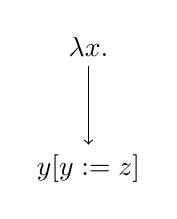
\begin{tikzpicture}[]

  \node[] (p0) [] {$\lambda x.$};
  \node[] (p1) [below=of p0] {$y[y := z]$};

  \path[->] (p0) edge (p1);
  
\end{tikzpicture}
\end{center}

\noindent
When we do the replacement, $y$ is replaced with $z$:

\begin{center}
\begin{tikzpicture}[]

  \node[] (p0) [] {$\lambda x.$};
  \node[] (p1) [below=of p0] {$z$};

  \path[->] (p0) edge (p1);
  
\end{tikzpicture}
\end{center}

\noindent
So the final result is:

\begin{equation}
\lambda x.z 
\end{equation}

\noindent
To put it all in one line:

\begin{equation}
M[y := N] = (\lambda x.y)[y := z] = \lambda x.(y[y := z]) = \lambda x.z
\end{equation}


%-------------------------------------------------------------------------------------------
%-------------------------------------------------------------------------------------------
\section{Nested Replacements}

Here is another example. Let $M$ be $\lambda x.(x y)$, and let $N$ be $\lambda z.z$:

\begin{align}
M = \lambda x.(x y) \\
N = \lambda z.z
\end{align}

\noindent
Suppose we want to replace every $y$ in $M$ with $N$:

\begin{equation}
M[y := N] = (\lambda x.(x y))[y: = (\lambda z.z)]
\end{equation}

\noindent
Here is a tree of the original expression:

\begin{center}
\begin{tikzpicture}[]

  \node[] (p0) [] {$\lambda x.$};
  \node[] (p1) [below=of p0] {$appl.$};
  \node[] (p2) [below left=of p1] {$x$};
  \node[] (p3) [below right=of p1] {$y$};

  \path[->] (p0) edge (p1);
  \path[->] (p1) edge (p2);
  \path[->] (p1) edge (p3);
  
\end{tikzpicture}
\end{center}

\noindent
To replace $y$ with $N$, we do it on the body of abstraction. The body is an application:

\begin{center}
\begin{tikzpicture}[]

  \node[] (p0) [] {$\lambda x.$};
  \node[] (p1) [below=of p0] {$appl.[y := (\lambda z.z)]$};
  \node[] (p2) [below left=of p1] {$x$};
  \node[] (p3) [below right=of p1] {$y$};

  \path[->] (p0) edge (p1);
  \path[->] (p1) edge (p2);
  \path[->] (p1) edge (p3);
  
\end{tikzpicture}
\end{center}

\noindent
To perform a substitution on an application, we know from above that we need to do the replacement on each of its child branches:

\begin{center}
\begin{tikzpicture}[]

  \node[] (p0) [] {$\lambda x.$};
  \node[] (p1) [below=of p0] {$appl.$};
  \node[] (p2) [below left=of p1] {$x[y := (\lambda z.z)]$};
  \node[] (p3) [below right=of p1] {$y[y := (\lambda z.z)]$};

  \path[->] (p0) edge (p1);
  \path[->] (p1) edge (p2);
  \path[->] (p1) edge (p3);
  
\end{tikzpicture}
\end{center}

\noindent
On the left branch, there is no $y$ to replace, but on the right branch there is. So the left branch doesn't change, and the right branch gets the replacement:

\begin{center}
\begin{tikzpicture}[]

  \node[] (p0) [] {$\lambda x.$};
  \node[] (p1) [below=of p0] {$appl.$};
  \node[] (p2) [below left=of p1] {$x$};
  \node[] (p3) [below right=of p1] {$\lambda z.z$};

  \path[->] (p0) edge (p1);
  \path[->] (p1) edge (p2);
  \path[->] (p1) edge (p3);
  
\end{tikzpicture}
\end{center}

\noindent
The result is this:

\begin{equation}
\lambda x.(x (\lambda z.z))
\end{equation}

\noindent
To put it all together:

\begin{align}
M[y := N] = \\
(\lambda x.(x y))[y := (\lambda z.z)] = \\
\lambda x.((x y)[y := (\lambda z.z)]) = \\
\lambda x.((x[y := (\lambda z.z)])(y[y := (\lambda z.z)])) = \\
\lambda x.(x (\lambda z.z))
\end{align}


%-------------------------------------------------------------------------------------------
%-------------------------------------------------------------------------------------------
\section{Naive Substitutions}

A \vocab{variable conflict} occurs when you do a replacement, and the replacement has (free) variables in it that are already used (bound) in the parent term. 

In the foregoing examples of abstraction substitutions, we had no variable conflicts. If you look back to each of the examples, you'll see that the original term used $x$s and $y$s, while the replacements used $z$s.

Variable conflicts can cause problems, so they need to be dealt with. Since our examples had no conflicts, we were able to \vocab{naively} substitute in the replacements, without worrying about conflicts.

Next, we will turn to the question of how to handle variable conflicts.


%-------------------------------------------------------------------------------------------
%-------------------------------------------------------------------------------------------
%-------------------------------------------------------------------------------------------
%-------------------------------------------------------------------------------------------
\chapter{Variable Capture}

When you perform a substitution in an abstraction, you take an abstraction $M$, and you end up grafting a new term $N$ onto various places on the tree.

But remember that the original term $M$ is an abstraction, and so it has a binding variable. That binding variable will bind any occurrences of itself on the tree. 

So, if $N$ has any free occurrences of that variable, when you graft $N$ onto the tree, those variables will be \vocab{captured} (bound) by the parent's binding expression. 

Variable capturing is not allowed in substitutions, but it is important to understand how it happens, and what exactly it results in.


%-------------------------------------------------------------------------------------------
%-------------------------------------------------------------------------------------------
\section{A Constant Abstraction}

Suppose we have a term $M$, which is $\lambda x.y$:

\begin{equation}
M = \lambda x.y
\end{equation}

\noindent
Here $x$ is the binding variable, but there is no $x$ in the body of the expression. Instead, the body of the expression is just $y$.

Think about what this computes. If you apply an argument to this and do the $\beta$-reduction, it will \textit{always} reduce to $y$. For example, suppose we want to replace $x$ with $z$:

\begin{equation}
\lambda x.y (z)
\end{equation}

\noindent
What happens when you do the $\beta$-reduction? Well, we take the argument, which is $z$, and we put in the place of every occurrence of $x$ in the body of the abstraction. There are no $x$s in the body, so we replace nothing. The result is thus: 

\begin{equation}
y
\end{equation}

\noindent
Now suppose we want to replace $x$ with, say, $5$. Strictly speaking, this is not a pure lambda term, because numbers are not part of our alphabet.\footnote{Of course, we can build up a number system using just the alphabet we have stipulated here, but that is not something we will do at this point. That happens when you start using the $\lambda$ calculus to build up more complex data structures like numbers, lists, and so on. You can do all of these things with the $\lambda$ calculus, but we will not do that at this point.} But let us use our imaginations for the moment, just to see the point:

\begin{equation}
\lambda x.y (5)
\end{equation}

\noindent
If we do the $\beta$-reduction, we get the same result. We take the argument, which is $5$, and we put it in the place of every occurrence of $x$ in the body of the abstraction. There are no $x$s in the body, so we replace nothing. The result is thus:

\begin{equation}
y
\end{equation}

\noindent
You can see that no matter what we provide as an argument for $x$, when we try to reduce this expression, it will always reduce to $y$. 

We can see even more clearly this by looking at the tree of this expression:

\begin{center}
\begin{tikzpicture}[]

  \node[] (p0) [] {$\lambda x$};
  \node[] (p1) [below=of p0] {$y$};

  \path[->] (p0) edge (p1);
  
\end{tikzpicture}
\end{center}

\noindent
Let us think about the binding and bound variables as slots instead of symbols. For instance, replace $x$ with square brackets:

\begin{center}
\begin{tikzpicture}[]

  \node[] (p0) [] {$\lambda [~~]$};
  \node[] (p1) [below=of p0] {$y$};

  \path[->] (p0) edge (p1);
  
\end{tikzpicture}
\end{center}

\noindent
We can see that whatever we put into the slot, there is no slot in the body to fill in. The body will always be $y$. So again, this abstraction will always reduce to $y$.

Sometimes we use a different way of speaking to make this same point: we say this abstraction always \vocab{returns} $y$. Also, because it always returns (or reduces down to) the same value, we say it returns a \vocab{constant}.


%-------------------------------------------------------------------------------------------
%-------------------------------------------------------------------------------------------
\section{A Naive Substitution}

Consider the constant abstraction we just discussed:

\begin{equation}
M = \lambda x.y
\end{equation}

\noindent
Here is a tree of it:

\begin{center}
\begin{tikzpicture}[]

  \node[] (p0) [] {$\lambda x$};
  \node[] (p1) [below=of p0] {$y$};

  \path[->] (p0) edge (p1);
  
\end{tikzpicture}
\end{center}

\noindent
Now suppose that we have another term $N$, which is just $x$:

\begin{equation}
N = x
\end{equation}

\noindent
Suppose that we want to take $M$ from before, and replace every occurrence of $y$ with $N$:

\begin{equation}
M[y := N]
\end{equation}

\noindent
Substitute $M$ and $N$ in, and you get this:

\begin{equation}
(\lambda x.y)[y := x]
\end{equation}

\noindent
To do this replacement in a naive way, we do the replacement in the body of the expression:

\begin{center}
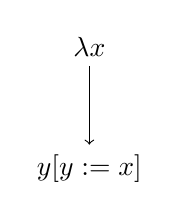
\begin{tikzpicture}[]

  \node[] (p0) [] {$\lambda x$};
  \node[] (p1) [below=of p0] {$y[y := x]$};

  \path[->] (p0) edge (p1);
  
\end{tikzpicture}
\end{center}

\noindent
And if you do the replacement, you get this:

\begin{center}
\begin{tikzpicture}[]

  \node[] (p0) [] {$\lambda x$};
  \node[] (p1) [below=of p0] {$x$};

  \path[->] (p0) edge (p1);
  
\end{tikzpicture}
\end{center}

\noindent
So the final result is:

\begin{equation}
\lambda x.x
\end{equation}

\noindent
To put it on one line:

\begin{equation}
(\lambda x.y)[y := x] = \lambda x.x
\end{equation}


%-------------------------------------------------------------------------------------------
%-------------------------------------------------------------------------------------------
\section{The New Abstraction}

The new abstraction we ended up with is this:

\begin{equation}
\lambda x.x
\end{equation}

\noindent
Think about what this term computes. The binding variable is $x$, but the body is $x$ too. So, if you provide an argument and do the $\beta$-reduction, you will replace the body with whatever value the argument is.

For example, suppose we want to replace $x$ with $z$:

\begin{equation}
\lambda x.x (z)
\end{equation}

\noindent
If we then do the $\beta$-reduction, we take $z$ and put in the place of the bound $x$, which gives us:

\begin{equation}
z
\end{equation}

\noindent
Let us imagine that we can replace $x$ with $5$ (again, this is not a pure $\lambda$ term, since numbers are not in our alphabet, but will use our imaginations).

\begin{equation}
\lambda x.x (5)
\end{equation}

\noindent
If we then do the $\beta$-reduction and replace $x$ in the body of the expression with $5$, we get:

\begin{equation}
5
\end{equation}

\noindent
No matter what value we provide as an argument, when we do the $\beta$-reduction, we will always return that same argument. This abstraction will always return the argument you give it.

We can see this even more clearly by looking at the tree:

\begin{center}
\begin{tikzpicture}[]

  \node[] (p0) [] {$\lambda x$};
  \node[] (p1) [below=of p0] {$x$};

  \path[->] (p0) edge (p1);
  
\end{tikzpicture}
\end{center}

\noindent
If we think about slots instead of symbols, we can see the structure of this abstraction:

\begin{center}
\begin{tikzpicture}[]

  \node[] (p0) [] {$\lambda [~~]$};
  \node[] (p1) [below=of p0] {$[~~]$};

  \path[->] (p0) edge (p1);
  
\end{tikzpicture}
\end{center}

\noindent
You can see from this that whatever value you put in the binding slot, you put that same value into the body of the expression.

So, this abstraction is \vocab{not constant}. The previous abstraction always returned $y$, but this one always returns whatever argument you give it.


%-------------------------------------------------------------------------------------------
%-------------------------------------------------------------------------------------------
\section{Variable Capture}

The new abstraction, $\lambda x.x$, has very different behavior from the previous one, $\lambda x.y$. As we saw, the previous abstraction is constant, but the new one is not.

So this replacement changed the behavior of the original in a quite substantial way.

The problem is that the value we swapped in got captured by the binding expression. In the first form of the expression, $\lambda x.y$, the $y$ was free. Again, look at the tree:

\begin{center}
\begin{tikzpicture}[]

  \node[] (p0) [] {$\lambda x$};
  \node[] (p1) [below=of p0] {$y$};

  \path[->] (p0) edge (p1);
  
\end{tikzpicture}
\end{center}

\noindent
The body is $y$, which is not bound by the binding variable $x$.

But then, we replaced $y$ with $x$:

\begin{center}
\begin{tikzpicture}[]

  \node[] (p0) [] {$\lambda x$};
  \node[] (p1) [below=of p0] {$x$};

  \path[->] (p0) edge (p1);
  
\end{tikzpicture}
\end{center}

\noindent
And at that point, the new value we put into the body of the expression got \vocab{captured} by the parent binding variable.


%-------------------------------------------------------------------------------------------
%-------------------------------------------------------------------------------------------
\section{Capture at Depth}

Capturing can happen at any level. A replacement might have any number of nested terms in it, and a variable that lives deep in a nested child might be the one that gets captured. 

Consider again our initial expression:

\begin{equation}
M = \lambda x.y
\end{equation}

\noindent
Here is the tree:

\begin{center}
\begin{tikzpicture}[]

  \node[] (p0) [] {$\lambda x$};
  \node[] (p1) [below=of p0] {$y$};

  \path[->] (p0) edge (p1);
  
\end{tikzpicture}
\end{center}

\noindent
Suppose that $N$ is a complex term, for instance:

\begin{equation}
N = (y (z (u x)))
\end{equation}

\noindent
Here is a tree of $N$:

\begin{center}
\begin{tikzpicture}[]

  \node[] (a0) [] {$appl.$};
  \node[] (a1) [below left=of a0] {$y$};
  \node[] (a2) [below right=of a0] {appl.};
  \node[] (a3) [below left=of a2] {$z$};
  \node[] (a4) [below right=of a2] {appl.};
  \node[] (a5) [below left=of a4] {$u$};
  \node[] (a6) [below right=of a4] {$x$};

  \path[->] (a0) edge (a1);
  \path[->] (a0) edge (a2);
  \path[->] (a2) edge (a3);
  \path[->] (a2) edge (a4);
  \path[->] (a4) edge (a5);
  \path[->] (a4) edge (a6);
  
\end{tikzpicture}
\end{center}

\noindent
Suppose we want to replace $y$ in the original expression with $N$:

\begin{equation}
M[y := N] = (\lambda x.y)[y := (y (z (u x)))]
\end{equation}

\noindent
The replacement happens in the body of the original expression, on the $y$:

\begin{center}
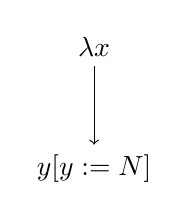
\begin{tikzpicture}[]

  \node[] (p0) [] {$\lambda x$};
  \node[] (p1) [below=of p0] {$y[y := N]$};

  \path[->] (p0) edge (p1);
  
\end{tikzpicture}
\end{center}

\noindent
So, if we replace $y$ with $N$, we graft the tree of $N$ on at that point:

\begin{center}
\begin{tikzpicture}[]

  \node[] (p0) [] {$\lambda x$};

  \node[] (a0) [below=of p0] {$appl.$};
  \node[] (a1) [below left=of a0] {$y$};
  \node[] (a2) [below right=of a0] {appl.};
  \node[] (a3) [below left=of a2] {$z$};
  \node[] (a4) [below right=of a2] {appl.};
  \node[] (a5) [below left=of a4] {$u$};
  \node[] (a6) [below right=of a4] {$x$};

  \path[->] (a0) edge (a1);
  \path[->] (a0) edge (a2);
  \path[->] (a2) edge (a3);
  \path[->] (a2) edge (a4);
  \path[->] (a4) edge (a5);
  \path[->] (a4) edge (a6);

  \path[->] (p0) edge (a0);
  
\end{tikzpicture}
\end{center}

\noindent
But notice that, at the far right child branch, we have an $x$. It was free before (when $N$ was all by itself), but now that it is grafted onto the tree for $M$, it ends up getting captured by the binding variable $x$ way at the top of the tree.



%-------------------------------------------------------------------------------------------
%-------------------------------------------------------------------------------------------
%-------------------------------------------------------------------------------------------
%-------------------------------------------------------------------------------------------
\chapter{Renaming}

In a substitution, you take a term $M$, and you replace every free occurrence of a variable $\phi$ in it with another term $N$. We write that like this:

\begin{equation}
M[\phi := N]
\end{equation}

\noindent
However, we cannot naively perform the substitution if any of the free variables in $N$ will get captured after the replacement. Before we do the replacement, we must change some variable names to avoid the conflict.

We can do this by replacing all the bound variables in the original term $M$ with fresh symbols that do not occur in $N$. After that, we can proceed with our naive substitition. 


%-------------------------------------------------------------------------------------------
%-------------------------------------------------------------------------------------------
\section{Fresh Symbols}

When you rename the bound variables, you must pick fresh symbols that do not occur in the term. We can define a fresh symbol as any symbol from our alphabet that is not among the bound variables of the term, nor among the free variables of the term.

\begin{definition}[Fresh symbols]
Let $M$ be a placeholder that can stand for any $\lambda$ term, and let $\phi$ be a placeholder that can stand for any symbol from the alphabet $V$. Then $\phi$ is fresh in $M$ (notated as $Fr(M)$) just in case the following conditions are satisfied:

\begin{itemize}
\item{$\phi \notin BV(M)$}
\item{$\phi \notin FV(M)$}
\end{itemize}
\end{definition}

\noindent
For example, suppose we have this term:

\begin{equation}
\lambda x.(x y)
\end{equation}

\noindent
Here are the variables we find in it:

\begin{itemize}
\item{Bound variables: $\{ x \}$}
\item{Free variables: $\{ y \}$}
\end{itemize}

\noindent
A fresh symbol will be any symbol from $V$ that is not in these two sets --- so any symbol from $V$ that is neither $x$ nor $y$. Here are some fresh symbols:

\begin{equation}
a, b, c, u, v, z, \ldots
\end{equation}

\noindent
\begin{remark}[The Barendregt Convention]
Henk Barendregt wrote an important book in the early 1980s called \textit{The Lambda Calculus: Its Syntax and Semantics}. There Barendregt suggested that all distinct bound variables in a $\lambda$ term should be fresh. That way, there are no variable conflicts. This is now often referred to as the \vocab{Barendregt convention}.
\end{remark}


%-------------------------------------------------------------------------------------------
%-------------------------------------------------------------------------------------------
\section{Renaming Procedure}

An abstraction has this form:

\begin{equation}
\lambda \phi.P
\end{equation}

\noindent
To rename the bound variable $\phi$ (and all occurrences of it in $P$), you proceed in three steps:

\begin{enumerate}
\item{Select a symbol that is fresh in $P$, call it $\psi$.}
\item{In $P$, replace all free occurrences of $\phi$ with $\psi$.}
\item{Replace $\lambda \phi$ with $\lambda \psi$.}
\end{enumerate}

\noindent
Think about each of these steps. 

In step (1), we pick a symbol that is fresh in $P$. That is, we pick a symbol from $Fr(P)$ --- a symbol that does not occur in $P$.

In step (2), we do a substitution of the sort we have already discussed. To use our notation, we do this:

\begin{equation}
P[\phi := \psi]
\end{equation}

\noindent
In step (3), we strip $\lambda \phi$ from the front of $P$, and we put $\lambda \psi$ in its place.

To put this all together, we start with this:

\begin{equation}
\lambda \phi.P
\end{equation}

\noindent
And we end up with this:

\begin{equation}
\lambda \psi.(P[\phi := \psi]), \text{ where } \phi \in Fr(P)
\end{equation}


%-------------------------------------------------------------------------------------------
%-------------------------------------------------------------------------------------------
\section{$\alpha$-conversion}

When we follow the procedure we just outlined, and rename the bound variables in an abstraction term, we call that an \vocab{$\alpha$-conversion} (or just ``alpha-conversion'' if you do not want to write the Greek letter $\alpha$). 

We can also say that an $\alpha$-converted term is \vocab{$\alpha$-congruent} with the original term, or that it is an \vocab{$\alpha$-variant} of the original term.

\begin{definition}[$\alpha$-conversion]
Let $M$ be an abstraction of the form $\lambda \phi.P$, and let $N$ be a placeholder for any $\lambda$ term. Then:

\begin{itemize}
\item{$N$ is an $\alpha$-conversion of $M$ just in case $\lambda \psi.(P[\phi := \psi])$, where $\psi \in Fr(P)$.} 
\item{If $N$ is an $\alpha$-conversion of $M$, then $N$ and $M$ are $\alpha$-congruent.}
\item{If $N$ is an $\alpha$-conversion of $M$, then $N$ is an $\alpha$-variant of $M$.}
\end{itemize}
\end{definition}


%-------------------------------------------------------------------------------------------
%-------------------------------------------------------------------------------------------
\section{A Simple Example}

Suppose we have an abstraction $M$, like this:

\begin{equation}
M = \lambda x.y
\end{equation}

\noindent
Here is the tree of $M$:

\begin{center}
\begin{tikzpicture}[]

  \node[] (p0) [] {$\lambda x$};
  \node[] (p1) [below=of p0] {$y$};

  \path[->] (p0) edge (p1);
  
\end{tikzpicture}
\end{center}

\noindent
Let us rename the bound variables in $M$ (i.e., let us perform an $\alpha$-conversion on $M$). 

If we follow our procedure, we first select a fresh symbol. The bound and free variables in $M$ are these:

\begin{equation}
BV(M) = \{ x \}, FV(M) = \{ y \}
\end{equation}

\noindent
So a fresh symbol $Fr(P)$ will be any symbol that is not $x$ or $y$. Let us pick $z$:

\begin{equation}
z \in Fr(P)
\end{equation}

\noindent
The second step is to replace every occurrence of $x$ with $z$ in the body of $M$. The body is $y$, so:

\begin{equation}
y[x := z]
\end{equation}

\noindent
Here it is on the tree:

\begin{center}
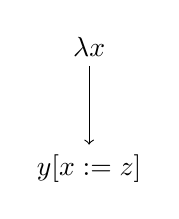
\begin{tikzpicture}[]

  \node[] (p0) [] {$\lambda x$};
  \node[] (p1) [below=of p0] {$y[x := z]$};

  \path[->] (p0) edge (p1);
  
\end{tikzpicture}
\end{center}

\noindent
Since there are no free occurrences of $x$ in $y$, $y$ remains unchanged:

\begin{center}
\begin{tikzpicture}[]

  \node[] (p0) [] {$\lambda x$};
  \node[] (p1) [below=of p0] {$y$};

  \path[->] (p0) edge (p1);
  
\end{tikzpicture}
\end{center}

\noindent
Finally, we remove $\lambda x$ and replace it with $\lambda z$:

\begin{center}
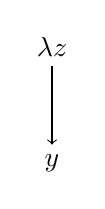
\begin{tikzpicture}[]

  \node[] (p0) [] {$\lambda z$};
  \node[] (p1) [below=of p0] {$y$};

  \path[->] (p0) edge (p1);
  
\end{tikzpicture}
\end{center}

\noindent
So, the final result is:

\begin{equation}
\lambda z.y
\end{equation}


%-------------------------------------------------------------------------------------------
%-------------------------------------------------------------------------------------------
\section{A Nested Example}

Note that step (2) involves a substitution, which we perform just as we discussed earlier. And of course, substitutions can involve nested substitutions. In such cases, you need to make sure to carry the substitution through to the nested children terms as well.

For example, suppose we have an abstraction $M$, like this:

\begin{equation}
M = \lambda x.(x y)
\end{equation}

\noindent
Here is the tree of $M$:

\begin{center}
\begin{tikzpicture}[]

  \node[] (p0) [] {$\lambda x$};
  \node[] (p1) [below=of p0] {appl.};
  \node[] (p2) [below left=of p1] {$x$};
  \node[] (p3) [below right=of p1] {$y$};

  \path[->] (p0) edge (p1);
  \path[->] (p1) edge (p2);
  \path[->] (p1) edge (p3);
  
\end{tikzpicture}
\end{center}

\noindent
Let us rename the bound variable $x$. First, we pick a fresh variable. Let us pick $z$ again:

\begin{equation}
z \in Fr(M)
\end{equation}

\noindent
Now let us replace every free occurrence of $x$ with $z$ in the body of $M$. That is:

\begin{equation}
\lambda x.((x y)[x := z])
\end{equation}

\noindent
Here it is on the tree:

\begin{center}
\begin{tikzpicture}[]

  \node[] (p0) [] {$\lambda x$};
  \node[] (p1) [below=of p0] {appl.$[x := z]$};
  \node[] (p2) [below left=of p1] {$x$};
  \node[] (p3) [below right=of p1] {$y$};

  \path[->] (p0) edge (p1);
  \path[->] (p1) edge (p2);
  \path[->] (p1) edge (p3);
  
\end{tikzpicture}
\end{center}

\noindent
To do a substitution on an application, we do the replacement on each of the child branches:

\begin{center}
\begin{tikzpicture}[]

  \node[] (p0) [] {$\lambda x$};
  \node[] (p1) [below=of p0] {appl.};
  \node[] (p2) [below left=of p1] {$x[x := z]$};
  \node[] (p3) [below right=of p1] {$y[x := z]$};

  \path[->] (p0) edge (p1);
  \path[->] (p1) edge (p2);
  \path[->] (p1) edge (p3);
  
\end{tikzpicture}
\end{center}

\noindent
On the left branch, $x$ gets replaced with $z$. On the right branch, there are no $x$s, so nothing happens:

\begin{center}
\begin{tikzpicture}[]

  \node[] (p0) [] {$\lambda x$};
  \node[] (p1) [below=of p0] {appl.};
  \node[] (p2) [below left=of p1] {$z$};
  \node[] (p3) [below right=of p1] {$y$};

  \path[->] (p0) edge (p1);
  \path[->] (p1) edge (p2);
  \path[->] (p1) edge (p3);
  
\end{tikzpicture}
\end{center}

\noindent
Finally, we remove $\lambda x$ and replace it with $\lambda z$:

\begin{center}
\begin{tikzpicture}[]

  \node[] (p0) [] {$\lambda z$};
  \node[] (p1) [below=of p0] {appl.};
  \node[] (p2) [below left=of p1] {$z$};
  \node[] (p3) [below right=of p1] {$y$};

  \path[->] (p0) edge (p1);
  \path[->] (p1) edge (p2);
  \path[->] (p1) edge (p3);
  
\end{tikzpicture}
\end{center}

\noindent
So, the final result is:

\begin{equation}
\lambda z.(z y)
\end{equation}


%-------------------------------------------------------------------------------------------
%-------------------------------------------------------------------------------------------
%-------------------------------------------------------------------------------------------
%-------------------------------------------------------------------------------------------
\chapter{Multiple Renames}

An abstraction can have children abstractions nested in its subterms. These can be renamed too, simply be repeating the renaming procedure for each abstraction.

To do multiple renames, always start from the innermost abstraction, and do the rename there first. Then work your way outwards and rename each successive outer abstraction as you come to them.

Suppose we have an abstraction $M$, that looks like this:

\begin{equation}
M = \lambda x.(x (\lambda y.(x z)))
\end{equation}

\noindent
Here is the tree of $M$:

\begin{center}
\begin{tikzpicture}[]

  \node[] (p0) [] {$\lambda x$};
  \node[] (p1) [below=of p0] {appl.};
  \node[] (p2) [below left=of p1] {$x$};
  \node[] (p3) [below right=of p1] {$\lambda y$};
  \node[] (p4) [below=of p3] {appl.};
  \node[] (p5) [below left=of p4] {$x$};
  \node[] (p6) [below right=of p4] {$z$};

  \path[->] (p0) edge (p1);
  \path[->] (p1) edge (p2);
  \path[->] (p1) edge (p3);
  \path[->] (p3) edge (p4);
  \path[->] (p4) edge (p5);
  \path[->] (p4) edge (p6);
  
\end{tikzpicture}
\end{center}

\noindent
The bound and free variables in this tree are these:

\begin{equation}
BV(M) = \{ x, y \}, FV(M) = \{ x, z \}
\end{equation}


%-------------------------------------------------------------------------------------------
%-------------------------------------------------------------------------------------------
\section{The First Pass}

To begin, let us rename the bound variable $y$. First, we select a fresh symbol. We cannot select $z$, since $z$ is among the free variables of $M$. Let us select $v_{1}$:

\begin{equation}
v_{1} \in Fr(M)
\end{equation}

\noindent
Next, let us substitute $v_{1}$ for every free occurrence of $y$ in the body of the abstraction:

\begin{center}
\begin{tikzpicture}[]

  \node[] (p0) [] {$\lambda x$};
  \node[] (p1) [below=of p0] {appl.};
  \node[] (p2) [below left=of p1] {$x$};
  \node[] (p3) [below right=of p1] {$\lambda y$};
  \node[] (p4) [below=of p3] {appl.$[y := v_{1}]$};
  \node[] (p5) [below left=of p4] {$x$};
  \node[] (p6) [below right=of p4] {$z$};

  \path[->] (p0) edge (p1);
  \path[->] (p1) edge (p2);
  \path[->] (p1) edge (p3);
  \path[->] (p3) edge (p4);
  \path[->] (p4) edge (p5);
  \path[->] (p4) edge (p6);
  
\end{tikzpicture}
\end{center}

\noindent
To perform a substitution on an application, we push the substitution down to each branch:

\begin{center}
\begin{tikzpicture}[]

  \node[] (p0) [] {$\lambda x$};
  \node[] (p1) [below=of p0] {appl.};
  \node[] (p2) [below left=of p1] {$x$};
  \node[] (p3) [below right=of p1] {$\lambda y$};
  \node[] (p4) [below=of p3] {appl.};
  \node[] (p5) [below left=of p4] {$x[y := v_{1}]$};
  \node[] (p6) [below right=of p4] {$z[y := v_{1}]$};

  \path[->] (p0) edge (p1);
  \path[->] (p1) edge (p2);
  \path[->] (p1) edge (p3);
  \path[->] (p3) edge (p4);
  \path[->] (p4) edge (p5);
  \path[->] (p4) edge (p6);
  
\end{tikzpicture}
\end{center}

\noindent
There are no free $y$s on either branch, so the bottom branches remain unchanged:

\begin{center}
\begin{tikzpicture}[]

  \node[] (p0) [] {$\lambda x$};
  \node[] (p1) [below=of p0] {appl.};
  \node[] (p2) [below left=of p1] {$x$};
  \node[] (p3) [below right=of p1] {$\lambda y$};
  \node[] (p4) [below=of p3] {appl.};
  \node[] (p5) [below left=of p4] {$x$};
  \node[] (p6) [below right=of p4] {$z$};

  \path[->] (p0) edge (p1);
  \path[->] (p1) edge (p2);
  \path[->] (p1) edge (p3);
  \path[->] (p3) edge (p4);
  \path[->] (p4) edge (p5);
  \path[->] (p4) edge (p6);
  
\end{tikzpicture}
\end{center}

\noindent
The last step in the rename is to replace $\lambda y$ with $\lambda v_{1}$:

\begin{center}
\begin{tikzpicture}[]

  \node[] (p0) [] {$\lambda x$};
  \node[] (p1) [below=of p0] {appl.};
  \node[] (p2) [below left=of p1] {$x$};
  \node[] (p3) [below right=of p1] {$\lambda v_{1}$};
  \node[] (p4) [below=of p3] {appl.};
  \node[] (p5) [below left=of p4] {$x$};
  \node[] (p6) [below right=of p4] {$z$};

  \path[->] (p0) edge (p1);
  \path[->] (p1) edge (p2);
  \path[->] (p1) edge (p3);
  \path[->] (p3) edge (p4);
  \path[->] (p4) edge (p5);
  \path[->] (p4) edge (p6);
  
\end{tikzpicture}
\end{center}

\noindent
The result is:

\begin{equation}
\lambda x.(x (\lambda v_{1}.(x z)))
\end{equation}

\noindent
Let us call this new term $N$:

\begin{equation}
N = \lambda x.(x (\lambda v_{1}.(x z)))
\end{equation}


%-------------------------------------------------------------------------------------------
%-------------------------------------------------------------------------------------------
\section{The Second Pass}

At this point, we can turn to the outer abstraction. First, we pick a fresh symbol. Let us select $v_{2}$:

\begin{equation}
v_{2} \in Fr(N)
\end{equation}

\noindent
Now we want to replace every free occurrence of $x$ with $v_{2}$ in the body of $N$:

\begin{center}
\begin{tikzpicture}[]

  \node[] (p0) [] {$\lambda x$};
  \node[] (p1) [below=of p0] {appl.$[x := v_{2}]$};
  \node[] (p2) [below left=of p1] {$x$};
  \node[] (p3) [below right=of p1] {$\lambda v_{1}$};
  \node[] (p4) [below=of p3] {appl.};
  \node[] (p5) [below left=of p4] {$x$};
  \node[] (p6) [below right=of p4] {$z$};

  \path[->] (p0) edge (p1);
  \path[->] (p1) edge (p2);
  \path[->] (p1) edge (p3);
  \path[->] (p3) edge (p4);
  \path[->] (p4) edge (p5);
  \path[->] (p4) edge (p6);
  
\end{tikzpicture}
\end{center}

\noindent
To do a substitution on an application, we push the replacement to each branch:

\begin{center}
\begin{tikzpicture}[]

  \node[] (p0) [] {$\lambda x$};
  \node[] (p1) [below=of p0] {appl.};
  \node[] (p2) [below left=of p1] {$x[x := v_{2}]$};
  \node[] (p3) [below right=of p1] {$\lambda v_{1}[x := v_{2}]$};
  \node[] (p4) [below=of p3] {appl.};
  \node[] (p5) [below left=of p4] {$x$};
  \node[] (p6) [below right=of p4] {$z$};

  \path[->] (p0) edge (p1);
  \path[->] (p1) edge (p2);
  \path[->] (p1) edge (p3);
  \path[->] (p3) edge (p4);
  \path[->] (p4) edge (p5);
  \path[->] (p4) edge (p6);
  
\end{tikzpicture}
\end{center}

\noindent
On the left branch, we can replace $x$ with $v_{2}$:

\begin{center}
\begin{tikzpicture}[]

  \node[] (p0) [] {$\lambda x$};
  \node[] (p1) [below=of p0] {appl.};
  \node[] (p2) [below left=of p1] {$v_{2}$};
  \node[] (p3) [below right=of p1] {$\lambda v_{1}[x := v_{2}]$};
  \node[] (p4) [below=of p3] {appl.};
  \node[] (p5) [below left=of p4] {$x$};
  \node[] (p6) [below right=of p4] {$z$};

  \path[->] (p0) edge (p1);
  \path[->] (p1) edge (p2);
  \path[->] (p1) edge (p3);
  \path[->] (p3) edge (p4);
  \path[->] (p4) edge (p5);
  \path[->] (p4) edge (p6);
  
\end{tikzpicture}
\end{center}

\noindent
On the right branch, we have an abstraction, so we push the substitution to the body:

\begin{center}
\begin{tikzpicture}[]

  \node[] (p0) [] {$\lambda x$};
  \node[] (p1) [below=of p0] {appl.};
  \node[] (p2) [below left=of p1] {$v_{2}$};
  \node[] (p3) [below right=of p1] {$\lambda v_{1}$};
  \node[] (p4) [below=of p3] {appl.$[x := v_{2}]$};
  \node[] (p5) [below left=of p4] {$x$};
  \node[] (p6) [below right=of p4] {$z$};

  \path[->] (p0) edge (p1);
  \path[->] (p1) edge (p2);
  \path[->] (p1) edge (p3);
  \path[->] (p3) edge (p4);
  \path[->] (p4) edge (p5);
  \path[->] (p4) edge (p6);
  
\end{tikzpicture}
\end{center}

\noindent
Now we have an application, so we push the replacement to its branches:

\begin{center}
\begin{tikzpicture}[]

  \node[] (p0) [] {$\lambda x$};
  \node[] (p1) [below=of p0] {appl.};
  \node[] (p2) [below left=of p1] {$v_{2}$};
  \node[] (p3) [below right=of p1] {$\lambda v_{1}$};
  \node[] (p4) [below=of p3] {appl.};
  \node[] (p5) [below left=of p4] {$x[x := v_{2}]$};
  \node[] (p6) [below right=of p4] {$z[x := v_{2}]$};

  \path[->] (p0) edge (p1);
  \path[->] (p1) edge (p2);
  \path[->] (p1) edge (p3);
  \path[->] (p3) edge (p4);
  \path[->] (p4) edge (p5);
  \path[->] (p4) edge (p6);
  
\end{tikzpicture}
\end{center}

\noindent
On the left, we can replace $x$ with $v_{2}$, and on the right, there is nothing to replace, so it remains unchanged:

\begin{center}
\begin{tikzpicture}[]

  \node[] (p0) [] {$\lambda x$};
  \node[] (p1) [below=of p0] {appl.};
  \node[] (p2) [below left=of p1] {$v_{2}$};
  \node[] (p3) [below right=of p1] {$\lambda v_{1}$};
  \node[] (p4) [below=of p3] {appl.};
  \node[] (p5) [below left=of p4] {$v_{2}$};
  \node[] (p6) [below right=of p4] {$z$};

  \path[->] (p0) edge (p1);
  \path[->] (p1) edge (p2);
  \path[->] (p1) edge (p3);
  \path[->] (p3) edge (p4);
  \path[->] (p4) edge (p5);
  \path[->] (p4) edge (p6);
  
\end{tikzpicture}
\end{center}

\noindent
The last step is we replace $\lambda x$ with $\lambda v_{2}$:

\begin{center}
\begin{tikzpicture}[]

  \node[] (p0) [] {$\lambda v_{2}$};
  \node[] (p1) [below=of p0] {appl.};
  \node[] (p2) [below left=of p1] {$v_{2}$};
  \node[] (p3) [below right=of p1] {$\lambda v_{1}$};
  \node[] (p4) [below=of p3] {appl.};
  \node[] (p5) [below left=of p4] {$v_{2}$};
  \node[] (p6) [below right=of p4] {$z$};

  \path[->] (p0) edge (p1);
  \path[->] (p1) edge (p2);
  \path[->] (p1) edge (p3);
  \path[->] (p3) edge (p4);
  \path[->] (p4) edge (p5);
  \path[->] (p4) edge (p6);
  
\end{tikzpicture}
\end{center}

\noindent
The final result is:

\begin{equation}
\lambda v_{2}.(v_{2} (\lambda v_{1}.(v_{2} z)))
\end{equation}

\noindent
Now we have completely renamed all the bound variables in the original term $M$, so that they are fresh. Neither of the bound variables $x$ or $y$ from before are present in this term. 


%-------------------------------------------------------------------------------------------
%-------------------------------------------------------------------------------------------
%-------------------------------------------------------------------------------------------
%-------------------------------------------------------------------------------------------
\chapter{Non-Naive Substitution in Abstractions}

Now that we have defined $\alpha$-conversions, we can reformulate how substitution works in abstractions, in a non-naive way. As we mentioned before: we first rename all bound variables in the term, and then we do the naive substitution.

Let us formulate this with our notation. An abstraction term $M$ has this form:

\begin{equation}
M = \lambda \phi.P
\end{equation}

\noindent
Before, we defined naive substitution as follows. Let $N$ be another term, and let $\psi$ be any symbol other than $\phi$ (so $\psi \not = \phi$). What we want to do is replace every occurrence of $\psi$ with $N$ in $M$, which we write like this:

\begin{equation}
M[\psi := N]
\end{equation}

\noindent
To do that naively, we simply do the replacement in the body of the expression, namely in $P$:

\begin{equation}
M[\psi := N] = \lambda \phi.(P[\psi := N])
\end{equation}

\noindent
However, we have now seen that we must first rename the bound variables in $P$, so that they are fresh. The bound variable here is $\phi$, so that is the one we want to replace. 

If we follow the procedure we outlined above, we first select a fresh symbol. Let $\xi$ be a placeholder that can stand for any symbol in $V$ that is fresh (so $\xi \not = \psi$ and $\xi \not = \phi$):

\begin{equation}
\xi \in FV(M)
\end{equation}

\noindent
Second, we replace every free occurrence of $\phi$ in $P$ with $\xi$:

\begin{equation}
P[\phi := \xi]
\end{equation}

\noindent
And third, we remove $\lambda \phi$ from the front and replace it with $\lambda \xi$:

\begin{equation}
\lambda \xi.(P[\phi := \xi])
\end{equation}

\noindent
The result of that will be an $\alpha$-variant of the original term $M$.

Now we can do the naive substitution, where we replace every $\psi$ with $N$. To write that, we simply tack $[\psi := N]$ onto the end:

\begin{equation}
(\lambda \phi.P)[\psi := N] = \lambda \xi.((P[\phi := \xi])[\psi := N])
\end{equation}
 
\noindent
The parentheses make it clear which replacements must happen first. First, we rename the bound $\phi$s to $\xi$s, and then we replace the $\psi$s with $N$s. 

Here is the whole rule:

\begin{multline}
\text{if $M = \lambda \phi.P$, $\psi \not = \phi$, and $\xi \in Fr(M)$, then: } \\ 
M[\psi := N] = (\lambda \phi.P)[\psi := N] = \\
\lambda \xi.((P[\phi := \xi])[\psi := N])
\end{multline}

\noindent
The notation here is cumbersome, but the basic point is simple: give the bound variables fresh names first, then do the naive substitution.


%-------------------------------------------------------------------------------------------
%-------------------------------------------------------------------------------------------
\section{An Example}

Suppose $M$ is $\lambda x.y$ and $N$ is $x$:

\begin{align}
M = \lambda x.y \\
N = x
\end{align}

\noindent
Suppose we want to replace every free occurrence of $y$ with $N$:

\begin{equation}
M[y := N]
\end{equation}

\noindent
Swap in $M$ and $N$, and you get:

\begin{equation}
(\lambda x.y)[y := x]
\end{equation}

\noindent
Here is the tree of $M$:

\begin{center}
\begin{tikzpicture}[]

  \node[] (p0) [] {$\lambda x$};
  \node[] (p1) [below=of p0] {$y$};

  \path[->] (p0) edge (p1);
  
\end{tikzpicture}
\end{center}

\noindent
If we were to do this substitution naively, we would replace $y$ with $x$, and the new $x$ would get captured by the binding expression $\lambda x$:

\begin{equation}
\lambda x.x
\end{equation}

\noindent
So before we do the substitution, we must rename the bound variable $x$. Let us pick a fresh symbol, $v_{1}$:

\begin{equation}
v_{1} \in Fr(M)
\end{equation}

\noindent
Now we want to replace every $x$ in the body with $v_{1}$:

\begin{center}
\begin{tikzpicture}[]

  \node[] (p0) [] {$\lambda x$};
  \node[] (p1) [below=of p0] {$y[x := v_{1}]$};

  \path[->] (p0) edge (p1);
  
\end{tikzpicture}
\end{center}

\noindent
There is nothing to replace here, so the body of the abstraction remains unchanged.

\begin{center}
\begin{tikzpicture}[]

  \node[] (p0) [] {$\lambda x$};
  \node[] (p1) [below=of p0] {$y$};

  \path[->] (p0) edge (p1);
  
\end{tikzpicture}
\end{center}

\noindent
The last step of the rename procedure is to remove $\lambda x$ and replace it with $\lambda v_{1}$:

\begin{center}
\begin{tikzpicture}[]

  \node[] (p0) [] {$\lambda v_{1}$};
  \node[] (p1) [below=of p0] {$y$};

  \path[->] (p0) edge (p1);
  
\end{tikzpicture}
\end{center}

\noindent
So, after the rename, the abstraction is this:

\begin{equation}
\lambda v_{1}.y
\end{equation}

\noindent
Now we can do our original substitution naively. We want to replace every $y$ with $x$:

\begin{equation}
(\lambda v_{1}.y)[y := x]
\end{equation}

\noindent
We do the substitution on the body the abstraction:

\begin{center}
\begin{tikzpicture}[]

  \node[] (p0) [] {$\lambda v_{1}$};
  \node[] (p1) [below=of p0] {$y[y := x]$};

  \path[->] (p0) edge (p1);
  
\end{tikzpicture}
\end{center}

\noindent
And once we do the replacement, we get:

\begin{center}
\begin{tikzpicture}[]

  \node[] (p0) [] {$\lambda v_{1}$};
  \node[] (p1) [below=of p0] {$x$};

  \path[->] (p0) edge (p1);
  
\end{tikzpicture}
\end{center}

\noindent
The final result is:

\begin{equation}
\lambda v_{1}.x
\end{equation}

\noindent
Now we have replaced $y$ in the body of the abstraction with $x$, but because we renamed the bound $x$ to $v_{1}$, there is no conflict. The $x$ we put into the body does not get captured.


%-------------------------------------------------------------------------------------------
%-------------------------------------------------------------------------------------------
%-------------------------------------------------------------------------------------------
%-------------------------------------------------------------------------------------------
\chapter{Multiple Non-Naive Substitutions}

Terms can be nested in other terms. So when we perform substitutions, we need to be careful to carry the substitutions out correctly, all the way down the branches, as many times as needed.

Suppose $M$ is $\lambda x.(x y)$ and $N$ is $\lambda x.z$:

\begin{align}
M = \lambda x.(x (\lambda x.(x y))) \\
N = \lambda x.z
\end{align}

\noindent
Suppose we want to replace every free occurrence of $y$ in $M$ with $N$:

\begin{equation}
M[y := N]
\end{equation}

\noindent
Swap in $M$ and $N$, and you get:

\begin{equation}
(\lambda x.(x (\lambda x.(x y))))[y := (\lambda x.z)]
\end{equation}

\noindent
Here is the tree of $M$:

\begin{center}
\begin{tikzpicture}[]

  \node[] (p0) [] {$\lambda x$};
  \node[] (p1) [below=of p0] {appl.};
  \node[] (p2) [below left=of p1] {$x$};
  \node[] (p3) [below right=of p1] {$\lambda x$};
  \node[] (p4) [below=of p3] {appl.};
  \node[] (p5) [below left=of p4] {$x$};
  \node[] (p6) [below right=of p4] {$y$};

  \path[->] (p0) edge (p1);
  \path[->] (p1) edge (p2);
  \path[->] (p1) edge (p3);
  \path[->] (p3) edge (p4);
  \path[->] (p4) edge (p5);
  \path[->] (p4) edge (p6);
  
\end{tikzpicture}
\end{center}

\noindent
Notice that there is a nested abstraction here, and both the child and parent abstractions bind $x$. But each has a different scope. The lowest $x$ is bound by the lower $\lambda x$, and the higher $x$ is bound by the higher $\lambda x$.

We can see this clearly if we think of slots in terms of variables. For the innermost $x$, I'll use square brackets $[~~]$, and for the outermost $x$, I'll use round braces $(~~)$. The tree looks like this:

\begin{center}
\begin{tikzpicture}[]

  \node[] (p0) [] {$\lambda (~~)$};
  \node[] (p1) [below=of p0] {appl.};
  \node[] (p2) [below left=of p1] {$(~~)$};
  \node[] (p3) [below right=of p1] {$\lambda [~~]$};
  \node[] (p4) [below=of p3] {appl.};
  \node[] (p5) [below left=of p4] {$[~~]$};
  \node[] (p6) [below right=of p4] {$y$};

  \path[->] (p0) edge (p1);
  \path[->] (p1) edge (p2);
  \path[->] (p1) edge (p3);
  \path[->] (p3) edge (p4);
  \path[->] (p4) edge (p5);
  \path[->] (p4) edge (p6);
  
\end{tikzpicture}
\end{center}

\noindent
This makes it clear which slots are bound where. The bottom slot $[~~]$ is bound by the bottom $\lambda [~~]$, and the top left slot $(~~)$ is bound by the top $\lambda (~~)$.

Before we do our substitution, we need to rename the bound variables. We always start renaming from the innermost abstraction, and we work our way outwards. So let us rename the bottom abstraction first. Let us pick a fresh symbol, $v_{1}$:

\begin{equation}
v_{1} \in Fr(M)
\end{equation}

\noindent
Then we replace every free $x$ in the body of the abstraction with $v_{1}$:

\begin{center}
\begin{tikzpicture}[]

  \node[] (p0) [] {$\lambda x$};
  \node[] (p1) [below=of p0] {appl.};
  \node[] (p2) [below left=of p1] {$x$};
  \node[] (p3) [below right=of p1] {$\lambda x$};
  \node[] (p4) [below=of p3] {appl.$[x := v_{1}]$};
  \node[] (p5) [below left=of p4] {$x$};
  \node[] (p6) [below right=of p4] {$y$};

  \path[->] (p0) edge (p1);
  \path[->] (p1) edge (p2);
  \path[->] (p1) edge (p3);
  \path[->] (p3) edge (p4);
  \path[->] (p4) edge (p5);
  \path[->] (p4) edge (p6);
  
\end{tikzpicture}
\end{center}

\noindent
This is an application, so we push the substitution to its branches:

\begin{center}
\begin{tikzpicture}[]

  \node[] (p0) [] {$\lambda x$};
  \node[] (p1) [below=of p0] {appl.};
  \node[] (p2) [below left=of p1] {$x$};
  \node[] (p3) [below right=of p1] {$\lambda x$};
  \node[] (p4) [below=of p3] {appl.};
  \node[] (p5) [below left=of p4] {$x[x := v_{1}]$};
  \node[] (p6) [below right=of p4] {$y[x := v_{1}]$};

  \path[->] (p0) edge (p1);
  \path[->] (p1) edge (p2);
  \path[->] (p1) edge (p3);
  \path[->] (p3) edge (p4);
  \path[->] (p4) edge (p5);
  \path[->] (p4) edge (p6);
  
\end{tikzpicture}
\end{center}

\noindent
On the left, we can replace $x$, and on the right, there is no change:

\begin{center}
\begin{tikzpicture}[]

  \node[] (p0) [] {$\lambda x$};
  \node[] (p1) [below=of p0] {appl.};
  \node[] (p2) [below left=of p1] {$x$};
  \node[] (p3) [below right=of p1] {$\lambda x$};
  \node[] (p4) [below=of p3] {appl.};
  \node[] (p5) [below left=of p4] {$v_{1}$};
  \node[] (p6) [below right=of p4] {$y$};

  \path[->] (p0) edge (p1);
  \path[->] (p1) edge (p2);
  \path[->] (p1) edge (p3);
  \path[->] (p3) edge (p4);
  \path[->] (p4) edge (p5);
  \path[->] (p4) edge (p6);
  
\end{tikzpicture}
\end{center}

\noindent
The last step of the rename is to replace the bottom $\lambda x$ with $\lambda v_{1}$:

\begin{center}
\begin{tikzpicture}[]

  \node[] (p0) [] {$\lambda x$};
  \node[] (p1) [below=of p0] {appl.};
  \node[] (p2) [below left=of p1] {$x$};
  \node[] (p3) [below right=of p1] {$\lambda v_{1}$};
  \node[] (p4) [below=of p3] {appl.};
  \node[] (p5) [below left=of p4] {$v_{1}$};
  \node[] (p6) [below right=of p4] {$y$};

  \path[->] (p0) edge (p1);
  \path[->] (p1) edge (p2);
  \path[->] (p1) edge (p3);
  \path[->] (p3) edge (p4);
  \path[->] (p4) edge (p5);
  \path[->] (p4) edge (p6);
  
\end{tikzpicture}
\end{center}

\noindent
Now we do a rename for the outer abstraction. Let us select a fresh variable $v_{2}$, and let us replace every free $x$ in the body of the abstraction with $v_{2}$:

\begin{center}
\begin{tikzpicture}[]

  \node[] (p0) [] {$\lambda x$};
  \node[] (p1) [below=of p0] {appl.$[x := v_{2}]$};
  \node[] (p2) [below left=of p1] {$x$};
  \node[] (p3) [below right=of p1] {$\lambda v_{1}$};
  \node[] (p4) [below=of p3] {appl.};
  \node[] (p5) [below left=of p4] {$v_{1}$};
  \node[] (p6) [below right=of p4] {$y$};

  \path[->] (p0) edge (p1);
  \path[->] (p1) edge (p2);
  \path[->] (p1) edge (p3);
  \path[->] (p3) edge (p4);
  \path[->] (p4) edge (p5);
  \path[->] (p4) edge (p6);
  
\end{tikzpicture}
\end{center}

\noindent
We can fast-forward a few steps, and push the replacement all the way down to all the branches:

\begin{center}
\begin{tikzpicture}[]

  \node[] (p0) [] {$\lambda x$};
  \node[] (p1) [below=of p0] {appl.};
  \node[] (p2) [below left=of p1] {$x[x := v_{2}]$};
  \node[] (p3) [below right=of p1] {$\lambda v_{1}$};
  \node[] (p4) [below=of p3] {appl.};
  \node[] (p5) [below left=of p4] {$v_{1}[x := v_{2}]$};
  \node[] (p6) [below right=of p4] {$y[x := v_{2}]$};

  \path[->] (p0) edge (p1);
  \path[->] (p1) edge (p2);
  \path[->] (p1) edge (p3);
  \path[->] (p3) edge (p4);
  \path[->] (p4) edge (p5);
  \path[->] (p4) edge (p6);
  
\end{tikzpicture}
\end{center}

\noindent
On the upper left branch, we can replace $x$, and on the bottom two branches there is no change:

\begin{center}
\begin{tikzpicture}[]

  \node[] (p0) [] {$\lambda x$};
  \node[] (p1) [below=of p0] {appl.};
  \node[] (p2) [below left=of p1] {$v_{2}$};
  \node[] (p3) [below right=of p1] {$\lambda v_{1}$};
  \node[] (p4) [below=of p3] {appl.};
  \node[] (p5) [below left=of p4] {$v_{1}$};
  \node[] (p6) [below right=of p4] {$y$};

  \path[->] (p0) edge (p1);
  \path[->] (p1) edge (p2);
  \path[->] (p1) edge (p3);
  \path[->] (p3) edge (p4);
  \path[->] (p4) edge (p5);
  \path[->] (p4) edge (p6);
  
\end{tikzpicture}
\end{center}

\noindent
The last step of the rename is to remove $\lambda x$ and put $\lambda v_{2}$ in its place:

\begin{center}
\begin{tikzpicture}[]

  \node[] (p0) [] {$\lambda v_{2}$};
  \node[] (p1) [below=of p0] {appl.};
  \node[] (p2) [below left=of p1] {$v_{2}$};
  \node[] (p3) [below right=of p1] {$\lambda v_{1}$};
  \node[] (p4) [below=of p3] {appl.};
  \node[] (p5) [below left=of p4] {$v_{1}$};
  \node[] (p6) [below right=of p4] {$y$};

  \path[->] (p0) edge (p1);
  \path[->] (p1) edge (p2);
  \path[->] (p1) edge (p3);
  \path[->] (p3) edge (p4);
  \path[->] (p4) edge (p5);
  \path[->] (p4) edge (p6);
  
\end{tikzpicture}
\end{center}

\noindent
So the final term after all bound variables have been renamed is this:

\begin{equation}
\lambda v_{2}.(v_{2} (\lambda v_{1}.(v_{1} y)))
\end{equation}

\noindent
Notice how the rename has made the expression a little easier to understand. There can be no confusion here about which $x$ is bound by which $\lambda x$. Here we have different (fresh) symbols for each binding, and so the tree looks a lot more like the tree we drew above with different slots.

At this point, we can do our naive substitution. Recall that $N$ is $\lambda x.z$, and that we want to replace every free $y$ with $N$:

\begin{center}
\begin{tikzpicture}[]

  \node[] (p0) [] {$\lambda v_{2}[y := (\lambda x.z)]$};
  \node[] (p1) [below=of p0] {appl.};
  \node[] (p2) [below left=of p1] {$v_{2}$};
  \node[] (p3) [below right=of p1] {$\lambda v_{1}$};
  \node[] (p4) [below=of p3] {appl.};
  \node[] (p5) [below left=of p4] {$v_{1}$};
  \node[] (p6) [below right=of p4] {$y$};

  \path[->] (p0) edge (p1);
  \path[->] (p1) edge (p2);
  \path[->] (p1) edge (p3);
  \path[->] (p3) edge (p4);
  \path[->] (p4) edge (p5);
  \path[->] (p4) edge (p6);

\end{tikzpicture}
\end{center}

\noindent
We have no variable conflicts (since we replaced all bound variables with fresh symbols), so we can proceed naively. We can fast-forward a few steps and push the substitution to all the branches:

\begin{center}
\begin{tikzpicture}[]

  \node[] (p0) [] {$\lambda v_{2}$};
  \node[] (p1) [below=of p0] {appl.};
  \node[] (p2) [below left=of p1] {$v_{2}[y := (\lambda x.z)]$};
  \node[] (p3) [below right=of p1] {$\lambda v_{1}$};
  \node[] (p4) [below=of p3] {appl.};
  \node[] (p5) [below left=of p4] {$v_{1}[y := (\lambda x.z)]$};
  \node[] (p6) [below right=of p4] {$y[y := (\lambda x.z)]$};

  \path[->] (p0) edge (p1);
  \path[->] (p1) edge (p2);
  \path[->] (p1) edge (p3);
  \path[->] (p3) edge (p4);
  \path[->] (p4) edge (p5);
  \path[->] (p4) edge (p6);

\end{tikzpicture}
\end{center}

\noindent
On the bottom right branch, we can remove $y$ and graft on $N$, but the rest of the replacements result in no change:

\begin{center}
\begin{tikzpicture}[]

  \node[] (p0) [] {$\lambda v_{2}$};
  \node[] (p1) [below=of p0] {appl.};
  \node[] (p2) [below left=of p1] {$v_{2}$};
  \node[] (p3) [below right=of p1] {$\lambda v_{1}$};
  \node[] (p4) [below=of p3] {appl.};
  \node[] (p5) [below left=of p4] {$v_{1}$};
  \node[] (p6) [below right=of p4] {$\lambda x$};
  \node[] (p7) [below=of p6] {$z$};

  \path[->] (p0) edge (p1);
  \path[->] (p1) edge (p2);
  \path[->] (p1) edge (p3);
  \path[->] (p3) edge (p4);
  \path[->] (p4) edge (p5);
  \path[->] (p4) edge (p6);
  \path[->] (p6) edge (p7);

\end{tikzpicture}
\end{center}



%-------------------------------------------------------------------------------------------
%-------------------------------------------------------------------------------------------
%-------------------------------------------------------------------------------------------
%-------------------------------------------------------------------------------------------
\chapter{Substitution (Formally)}

With the above information at hand, we can define substitution formally. The format for any substitution is:

\begin{equation}
M[\phi := N]
\end{equation}

\noindent
where $M$ and $N$ are placeholders that can stand for any $\lambda$ term, and $\phi$ is a placeholder that can stand for any symbol in the alphabet $V$.

There are three types of $\lambda$ terms: variable terms, application terms, and abstraction terms. Substitution works differently for each:

\begin{itemize}

\item{\vocab{Variables} --- If the variable is just $\phi$, you replace it with $N$, otherwise you make no change. So if $M$ = $\phi$, you replace that with $N$. If $M$ is some other variable, $\psi$, where $\psi \not = \phi$, then you leave it as $\psi$.}

\item{\vocab{Applications} --- You push the substitution into each of the child terms. If $M$ is $(P Q)$, you do the replacement on each: $(P[\phi := N])(Q[\phi := N])$.}

\item{\vocab{Abstractions} --- This is the complicated one. $M$ has the form $\lambda \psi.P$, and you proceed in two stages. First, you replace all the bound variables with fresh symbols. So, you replace $\psi$ with a fresh symbol, $\xi$ (i.e., $\xi \in Fr(M)$). That is to say, $\lambda \psi.P$ gets converted to $\lambda \xi.(P[\psi := \xi])$. And of course, $P$ itself might have further nested abstractions, and you need to walk down the tree and re-apply this rule: replace all bound variables with fresh symbols. Then you can move to the second stage: you do a naive substitution and replace $\phi$ in the body of the expression with $N$ --- i.e., $\lambda \xi.(P[\psi := \xi]([\phi := N]))$.}

\end{itemize}

\noindent
Here is the full definition:

\begin{definition}[Substitution]
Let $M$, $N$, $P$, and $Q$ be placeholders that can stand for any $\lambda$ term, and let $\phi$, $\psi$, and $\xi$ be placeholders that can stand for any symbol in the alphabet $V$. Then substitution is defined as the result of taking a term $M$, and replacing every free occurrence of $\phi$ in it with another term $N$. This is notated as $M[\phi := N]$. The replacement must proceed according to the following rules:

\begin{itemize}
\item{If $M$ is $(\phi)$, then $M[\phi := N] = N$.}
\item{If $M$ is $(\psi)$ and $\psi \not = \phi$, then $M[\phi := N] = M$.}
\item{If $M$ is $(PQ)$, then $M[\phi := N] = ((P[\phi := N])(Q[\phi := N]))$.}
\item{If $M$ is $\lambda \psi.P$, then $M[\phi := N] = \lambda \xi.(P[\psi := \xi]([\phi := N]))$, where $\xi \in Fr(M)$.}
\end{itemize}
\end{definition}



%-------------------------------------------------------------------------------------------
%-------------------------------------------------------------------------------------------
%-------------------------------------------------------------------------------------------
%-------------------------------------------------------------------------------------------
\chapter{Equivalence}


%-------------------------------------------------------------------------------------------
%-------------------------------------------------------------------------------------------
\section{Reflexivity, Symmetry, and Transitivity}

In mathematics and logic, we can compare two objects to each other in various ways. There are three properties of relationships that we often look at:

\begin{itemize}

\item{Some comparisons are \vocab{symmetric}, which means it goes both ways. If John is the brother of Thomas, it goes the other way too: Thomas is the brother is John. Not all comparisons are symmetric. If John is taller than Thomas, it does not follow that Thomas is taller than John.}

\item{Some comparisons are \vocab{reflexive}, which means the objects can be compared to themselves too. If John is as smart as Thomas, we can say that John is as smart as himself too. Of course, we may not normally say things like ``John is as smart as himself,'' but it is a true statement (in fact, it seems like it couldn't be false). Not all comparisons are reflexive. If Harold is a parent of John, it does not follow that Harold is a parent of Harold.}

\item{Some comparisons are \vocab{transitive}, which means they can be chained. If John is taller than Thomas and Thomas is taller than Sally, then John is taller than Sally. Not all comparisons are transitive. If my left arm is attached directly to my body and my body is attached directly to my right arm, it does not follow that my left arm is attached directly to my right arm (on the contrary, my body is in between them).}

\end{itemize}

\noindent
We can put these statements more formally, by describing them as general properties of relations.

\begin{definition}[Reflexivity, Symmetry, Transitivity]
Let $R$ be a relation, and let $x$, $y$, and $z$ be placeholders that can stand for any items related by $R$. Then:

\begin{itemize}

\item{$R$ is reflexive: if $x$ is related to $y$ by $R$, then $x$ is related to $x$ by $R$.}

\item{$R$ is symmetric: if $x$ is related to $y$ by $R$, then $y$ is related to $x$ by $R$.}

\item{$R$ is transitive: if $x$ is related to $y$ by $R$ and $y$ is related to $z$ by $R$, then $x$ is related to $z$ by $R$.}

\end{itemize} 

\end{definition}

%-------------------------------------------------------------------------------------------
%-------------------------------------------------------------------------------------------
\section{Definition of Equivalence}

When objects are compared in such a way that the comparison is all of the above --- that is, it is reflexive, symmetric, and transitive --- then we say the objects are \vocab{equivalent}. The definition of equivalence is precisely any relationship that is reflexive, symmetric, and transitive.

\begin{definition}[Equivalence]
For any relation $R$, $R$ is an equivalence relation just in case $R$ is reflexive, symmetric, and transitive.
\end{definition}


%-------------------------------------------------------------------------------------------
%-------------------------------------------------------------------------------------------
\section{Equivalence and Identity}

Equivalence is not the same as identity. To say that two objects are equivalent is not the same as saying that they are identical. 

\begin{itemize}
\item{The morning star and the evening star are the very same object, namely the planet Venus. So they are identical.}
\item{To prove that you can work in the United States, you need to show one of two things: (i) a passport, or (ii) a birth certificate and a state-issued driver's license. These two options are not identical, but they are equivalent, for the purposes of proving that you are allowed to work in the United States.}
\end{itemize}

\noindent
Mathematicians and logicians sometimes use an equals sign ($=$) ambiguously. Sometimes they use it to mean identity. For instance, in arithmetic, we might see this:

\begin{equation}
7 = 7
\end{equation}

\noindent
This is identity. The number 7 is the same object as the number 7, or the value 7 is identical to the value 7.

But the following is equivalence, not identity:

\begin{equation}
5 + 2 = 7
\end{equation}

\noindent
These are computationally equivalent, because if you solve on the left side of the equation you get an identical value. But $5 + 2$ is obviously not identical to $7$.

To help keep things clear, we will reserve an equals sign ($=$) for identity, and we will use a three-line equals sign ($\equiv$) for equivalence. So:

\begin{equation}
5 + 2 \equiv 7
\end{equation}

\noindent
And:

\begin{equation}
7 = 7
\end{equation}



%-------------------------------------------------------------------------------------------
%-------------------------------------------------------------------------------------------
%-------------------------------------------------------------------------------------------
%-------------------------------------------------------------------------------------------
\chapter{Equivalent $\alpha$-Variants (Informally)}

In the $\lambda$ calculus, $\alpha$-variants are equivalent. We can see this informally by looking at how they compute the same results, and how they have the same structure.


%-------------------------------------------------------------------------------------------
%-------------------------------------------------------------------------------------------
\section{Computationally Equivalent}

Any $\alpha$-variants will compute the same result. For instance, consider this term:

\begin{equation}
\lambda x.x
\end{equation}

\noindent
Computationally, this will return whatever argument we provide to it. For instance, suppose we apply it to $y$:

\begin{equation}
(\lambda x.x) y  
\end{equation}

\noindent
If you do the $\beta$-reduction, you get $y$:

\begin{equation}
(\lambda x.x) y = y
\end{equation}

\noindent
If you apply it to a different argument, say $z$, you get $z$:

\begin{equation}
(\lambda x.x) z = z  
\end{equation}

\noindent
Now suppose we replace the bound variables with fresh symbols. For instance, let's replace $x$ with $a$:

\begin{equation}
\lambda a.a
\end{equation}

\noindent
This new term behaves the same way. It always returns the argument. We can do the same two computations as above, and the result is the same:

\begin{align}
(\lambda a.a) y = y \\  
(\lambda a.a) z = z
\end{align}

\noindent
Let's rename it again. Let's pick $v_{10}$:

\begin{equation}
(\lambda v_{10}.v_{10})
\end{equation}

\noindent
Again, this computes the same results:

\begin{align}
(\lambda v_{10}.v_{10}) y = y \\  
(\lambda v_{10}.v_{10}) z = z
\end{align}

\noindent
Here is another example. Take this term:

\begin{equation}
\lambda x.(x y)
\end{equation}

\noindent
Let's apply this to $a$, and then to $b$:

\begin{align}
(\lambda x.(x y)) a = (a y) \\
(\lambda x.(x y)) b = (b y)
\end{align}

\noindent
When we compute the results here, we can see that this abstraction always returns the argument with $y$.

Now rename the bound variables to, say, $v_{1}$. We get the same results:

\begin{align}
(\lambda v_{1}.(v_{1} y)) a = (a y) \\
(\lambda v_{1}.(v_{1} y)) b = (b y)
\end{align}

\noindent
Try more renamings. We still get the same results:

\begin{align}
(\lambda v_{2}.(v_{2} y)) a = (a y) \\
(\lambda v_{2}.(v_{2} y)) b = (b y) \\
\ldots \\
(\lambda v_{4}.(v_{4} y)) a = (a y) \\
(\lambda v_{4}.(v_{4} y)) b = (b y) \\
\ldots
\end{align}


%-------------------------------------------------------------------------------------------
%-------------------------------------------------------------------------------------------
\section{Same Structure}

If we think of the bound variables as slots instead of symbols, it is easy to see that $\alpha$-variants have the same structure. Take the abstraction we had above:

\begin{equation}
\lambda x.(x y)
\end{equation}

\noindent
Here it is as a tree:

\begin{center}
\begin{tikzpicture}[]

  \node[] (p0) [] {$\lambda x$};
  \node[] (p1) [below=of p0] {appl.};
  \node[] (p2) [below left=of p1] {$x$};
  \node[] (p3) [below right=of p1] {$y$};

  \path[->] (p0) edge (p1);
  \path[->] (p1) edge (p2);
  \path[->] (p1) edge (p3);

\end{tikzpicture}
\end{center}

\noindent
If we think of the $x$s as slots, we can see the structure of this expression very clearly:

\begin{center}
\begin{tikzpicture}[]

  \node[] (p0) [] {$\lambda [~~]$};
  \node[] (p1) [below=of p0] {appl.};
  \node[] (p2) [below left=of p1] {$[~~]$};
  \node[] (p3) [below right=of p1] {$y$};

  \path[->] (p0) edge (p1);
  \path[->] (p1) edge (p2);
  \path[->] (p1) edge (p3);

\end{tikzpicture}
\end{center}

\noindent
No matter which fresh symbols we put in the place of the bound $x$s, the result will have this same structure.

This is also true when there are multiple, nested bindings. Consider the following $\lambda$ term:

\begin{equation}
\lambda x.(\lambda y.(x y))
\end{equation}

\noindent
Here it is as a tree:

\begin{center}
\begin{tikzpicture}[]

  \node[] (p0) [] {$\lambda x$};
  \node[] (pb) [below=of p0] {$\lambda y$};
  \node[] (p1) [below=of pb] {appl.};
  \node[] (p2) [below left=of p1] {$x$};
  \node[] (p3) [below right=of p1] {$y$};

  \path[->] (p0) edge (pb);
  \path[->] (pb) edge (p1);
  \path[->] (p1) edge (p2);
  \path[->] (p1) edge (p3);

\end{tikzpicture}
\end{center}

\noindent
If we use square brackets for the $x$ slots and round braces for the $y$ slots, we can see the structure of this term:

\begin{center}
\begin{tikzpicture}[]

  \node[] (p0) [] {$\lambda [~~]$};
  \node[] (pb) [below=of p0] {$\lambda (~~)$};
  \node[] (p1) [below=of pb] {appl.};
  \node[] (p2) [below left=of p1] {$[~~]$};
  \node[] (p3) [below right=of p1] {$(~~)$};

  \path[->] (p0) edge (pb);
  \path[->] (pb) edge (p1);
  \path[->] (p1) edge (p2);
  \path[->] (p1) edge (p3);

\end{tikzpicture}
\end{center}

\noindent
Here too, we can see that no matter which fresh symbols we put in the appropriate slots, the structure remains the same.


%-------------------------------------------------------------------------------------------
%-------------------------------------------------------------------------------------------
%-------------------------------------------------------------------------------------------
%-------------------------------------------------------------------------------------------
\chapter{Specifying Types}


Type systems provide a way of stipulating a variety of things: 

\begin{itemize}
\item{You can stipulate what types of \vocab{values} are available for use in computations: e.g., numbers, prices, phone numbers.}
\item{You can stipulate which types of \vocab{arguments} are valid inputs to an abstraction.}
\item{You can stipulate which types of \vocab{results} an expression can compute.}
\end{itemize}


%-------------------------------------------------------------------------------------------
%-------------------------------------------------------------------------------------------
\section{Types}

Not all values are the same type of value. Compare the following values:

\begin{center}
5 \\
Sally \\
(765) 546-2378 \\
\$2.50
\end{center}

\noindent
The first item is a number (the number 5), the second item is a name (the name Sally), the third item is a domestic US phone number, and the fourth item is a unit of money, in USD.

For computational purposes, we can organize values into types, and give the types names. For instance, we could stipulate a type called \textit{USD-unit}, and say that it is the collection of all values that are units of money in USD. Then we can say that \$2.50 is a value of this type precisely because it is contained in the \textit{USD-unit} collection.

Similarly, we could stipulate a type called \textit{phone-numbers}, and say that it contains all domestic US phone-numbers. The value (765) 546-2378 is a value of this type precisely because it is contained in this collection.


%-------------------------------------------------------------------------------------------
%-------------------------------------------------------------------------------------------
\section{Restricting Inputs}

Once we have declared a set of types that are available for computations, we can stipulate which types computations can work with.

Suppose you have an abstraction that looks something like this:

\begin{equation}
\text{Replace ``price'' in (multiply 2 by price)}
\end{equation}

\noindent
As we know, we can stipulate a value to put in place of ``price,'' for example ``5'':

\begin{equation}
\text{Replace ``price'' with ``5'' in (multiply 2 by price)}
\end{equation}

\noindent
When you do the replacement, you get this:

\begin{equation}
\text{multiply 2 by 5}
\end{equation}

\noindent
But what if you replace ``price'' with, say, ``Tom''?

\begin{equation}
\text{Replace ``price'' with ``Tom'' in (multiply 2 by price)}
\end{equation}

\noindent
When you do that replacement, you get this:

\begin{equation}
\text{multiply 2 by Tom}
\end{equation}

\noindent
The untyped $\lambda$ calculus allows this, because as far as it is concerned, it just manipulates symbols.

However, we might want to restrict the types of values you can put in the place of ``price.'' We might want to say something like this: ``you can replace `price' only with a unit in USD.'' 

To do that, we could write this out explicitly:

\begin{equation}
\text{Replace ``price'' with a USD-unit in (multiply 2 by price)}
\end{equation}

\noindent
Now it is clear that ``Tom'' doesn't fit in the place of ``price''. If you try it, you get this:

\begin{equation}
\text{Replace ``price'' with the USD-unit ``Tom'' in (multiply 2 by price)}
\end{equation}

\noindent
And that makes no sense, because ``Tom'' is not a unit of USD. However, if you select a unit of USD, then your expression does make sense:

\begin{equation}
\text{Replace ``price'' with the USD-unit ``\$2.50'' in (multiply 2 by price)}
\end{equation}


%-------------------------------------------------------------------------------------------
%-------------------------------------------------------------------------------------------
\section{Specifying Outputs}

We can specify the type of the result (or output) of a calculation too.

Suppose we want to calculate the total cost of $x$ pounds of sand. We know that each pound costs \$2.50. To do that calculation, we would multiply the number of pounds by \$2.50.

So, suppose we encode this with an abstraction. Like this:

\begin{equation}
\text{replace ``lbs'' in (multiply lbs by \$2.50)}
\end{equation}

\noindent
Obviously it would make no sense to put something like ``Tom'' in the place of ``lbs'':

\begin{equation}
\text{replace ``lbs'' with ``Tom'' in (multiply lbs by \$2.50)}
\end{equation}

\noindent
So, we stipulate that the type of the replacement should be a unit of pounds:

\begin{equation}
\text{replace ``lbs'' with a lbs-unit in (multiply lbs by \$2.50)}
\end{equation}

\noindent
Now we can only put in lbs units. For instance, ``2 lbs'':

\begin{equation}
\text{replace ``lbs'' with the lbs-unit ``2 lbs'' in (multiply lbs by \$2.50)}
\end{equation}

\noindent
If we do that replacement, we get:

\begin{equation}
\text{multiply 2 lbs by \$2.50}
\end{equation}

\noindent
Suppose that we go on to perform the calculation here --- we multiply 2 (lbs) by 2.50 (USD). That gives us the total cost of the sand:

\begin{equation}
\$5.00
\end{equation}

\noindent
This value is a unit of USD. So, the result of this calculation has a type too: it is a USD unit.

To specify this, we could explicitly say it in our expression:

\begin{equation}
\text{replace ``lbs'' with a lbs-unit in (multiply lbs by \$2.50) to get a USD-unit}
\end{equation}

\noindent
Now it is clear which type of input goes in, and which type of output comes out.


%-------------------------------------------------------------------------------------------
%-------------------------------------------------------------------------------------------
\section{Arrows}

We can specify input-output pair of types with an arrow. For instance, for the last expression, we can say this:

\begin{equation}
\text{\textit{lbs-units} $\rightarrow$ \textit{USD-units}}
\end{equation}

\noindent
This is a way to specify the type of the expression. Hence: 

\begin{itemize}
\item{Collections are ways to specify the type of \vocab{values}.} 
\item{Arrows are ways to specify the type of \vocab{expressions}.}
\end{itemize}

\noindent
Let us use this vocabulary. Take the expression we formulated a moment ago: 

\begin{equation}
\text{replace ``lbs'' with a lbs-unit in (multiply lbs by \$2.50) to get a USD-unit}
\end{equation}

\noindent
This is of the following type: \textit{lbs-units} $\rightarrow$ \textit{USD-units}, which means it is the type of expression that takes lbs-units for input, and it produces USD-units as output.

Many computations implicitly assume some sort of arrow typing like this. Consider the sort of basic arithmetic you might have done in school. For instance:

\begin{equation}
x + 5
\end{equation}

\noindent
It is often not stated explicitly, but the unwritten assumption is that you can only put a number in the place of $x$, and that the result will also be a number. So this expression has the type:

\begin{equation}
\text{\textit{number} $\rightarrow$ \textit{number}}
\end{equation}


%-------------------------------------------------------------------------------------------
%-------------------------------------------------------------------------------------------
\section{Collections and Arrows}

In the foregoing, we did two things when it comes to types. 

\begin{itemize}

\item{We stipulated that there are certain types of values, i.e., collections of certain values. For instance, we said that there are USD-units, or lbs-units.}

\item{We stipulated that expressions take inputs of a certain type, and they produce outputs of a certain type. For instance, we said that our ``multiply lbs by \$2.50'' expression takes lbs-units for input, and it produces USD-units as output.}

\end{itemize}

\noindent
We have names for these.

\begin{itemize}

\item{We will call collections of values \vocab{collection} types, because each type is a collection of particular values. For instance, ``USD-unit'' is a collection type.}

\item{We will call the input-output pairs \vocab{arrow} types, because they show how you go from one type of value to another. For instance, \textit{lbs-unit} $\rightarrow$ \textit{USD-units} is an arrow type.}

\end{itemize}

\noindent
Simple type theory provides a way for us to specify these sorts of type restrictions (though of course in a formal way, building on top of the $\lambda$ calculus).


%-------------------------------------------------------------------------------------------
%-------------------------------------------------------------------------------------------
%-------------------------------------------------------------------------------------------
%-------------------------------------------------------------------------------------------
\chapter{Simple Types (Informally)}

Let us think more about the two sorts of types we encountered before: collection types and arrow types.


%-------------------------------------------------------------------------------------------
%-------------------------------------------------------------------------------------------
\section{Collection Types}

What are collection types? Here is some terminology:

\begin{itemize}

\item{A collection type is an exactly specified collection of items.} 

\item{We say that the items in the collection are the \vocab{inhabitants} of the type.}

\end{itemize}

\noindent
Some obvious examples are the different number types we learn about in school:

\begin{itemize}

\item{The set of natural numbers, written as: $\mathbb{N}$. This is an exactly specified collection: it consists of all and only the natural numbers $0, 1, 2, \ldots$ It does not include any negative numbers, fractions, or decimals.}

\item{The set of integers, written as $\mathbb{Z}$. This includes the natural numbers plus all negative whole numbers: $\ldots, -3, -2, -1, 0, 1, 2, 3 \ldots$}

\item{The set of all fractions, which are called the ``rational numbers'' (from ``ratio'') because they can be represented as a quotient. Hence, the symbol for the rational numbers is $\mathbb{Q}$ (for ``quotient'').}

\end{itemize}

\noindent
You can create your own collection type, for any purpose whatever, simply by specifying a collection. The only requirement is that it must be exactly specified, and by that, I mean you must specify exactly which items belong in the collection. Here are some examples:

\begin{itemize}

\item{The colors of the rainbow: red, orange, yellow, green, blue, and purple.}

\item{The 2018 Porsche models: the 911, the Boxster, the Cayman, the Cayenne, the Macan, and the Panamera.}

\end{itemize}

\noindent
Collection types may have only a few inhabitants, like the two collections just mentioned. It is easy to specify such collections: you just list their inhabitants.

But some collection types have an infinite number of inhabitants --- e.g., any of the number types we just mentioned, like integers or natural numbers.

For those that have an infinite number of inhabitants, you obviously cannot list them all. In that case, to define a collection type, you need to specify an exact way to \vocab{construct} each and every inhabitant of the type.

For example, any natural number can be constructed with a zero and a successor operation. To construct the first number after zero, you take the successor of zero. To construct the next number you take the successor of the successor of zero. To construct the next number you take the successor of the successor of the successor of zero, and so on.


%-------------------------------------------------------------------------------------------
%-------------------------------------------------------------------------------------------
\section{Arrow Types}

The second kind of type is the arrow. The inhabitants of an \vocab{arrow} type are mappings from one type to another.

Suppose we have two collection types: one is a collection of \textit{employees}, and the other is a collection of \textit{phone-numbers}. What we want to do is connect employees to phone numbers.

To do that, we might take a piece of paper, write all the employees on the left, and all the phone numbers on the right. Then we could draw an arrow from each employee to a phone number. Something like this:

\begin{center}
\begin{tikzpicture}[]

  \node[] (a0) [label=left:{Sally Farnston}] {};
  \node[] (a1) [below=.25cm of a0,label=left:{Harold Moore}] {};
  \node[] (a2) [below=.25cm of a1,label=left:{Jennifer Kowana}] {};
  \node[] (a3) [below=.25cm of a2,label=left:{$\ldots$}] {};
  
  \node[] (b0) [right=2cm of a0,label=right:{567-2876}] {};
  \node[] (b1) [right=2cm of a1,label=right:{227-9600}] {};
  \node[] (b2) [right=2cm of a2,label=right:{545-0428}] {};
  \node[] (b3) [right=2cm of a3,label=right:{$\ldots$}] {};

  \path[->] (a0) edge (b1);
  \path[->] (a1) edge (b2);
  \path[->] (a2) edge (b0);

\end{tikzpicture}
\end{center}

\noindent
This is a mapping from employees to phone numbers. In set theory, we call this a \vocab{function}. It is essentially a look-up table --- to each item on the left, you assign one item on the right --- so that, for any given an employee, you can look up their phone number.

Of course, we could make a variety of different mappings between these two collections. We could draw the lines differently so that, say, Sally's phone number is 567-2876 instead of 227-9600.

But all such mappings have one thing in common: they map \textit{employees} to \textit{phone-numbers}. If we collect together all mappings from employees to phone numbers, we have an arrow type. 

To specify this type, we write it like this:

\begin{equation}
\text{\textit{employees} $\rightarrow$ \textit{phone-numbers}}
\end{equation}




% -----------------------------------------------
% -----------------------------------------------
% -----------------------------------------------
% -----------------------------------------------
\chapter{Constructing Types}

Let us begin to formulate the simple typed $\lambda$ calculus. Instead of writing ``simply typed $\lambda$,'' I will write ``$\lambda\rightarrow$.''


% -----------------------------------------------
% -----------------------------------------------
\section{An Alphabet for Type Variables}

A collection type is an exactly specified collection of values. We can give names to collection types. In our earlier example, we named the collection of USD values \textit{USD-unit}. 

We do not need to work with long names. We can just use single-character symbols. Let us establish an alphabet of symbols we can use to construct type names. We will call these \vocab{type variables}.

\begin{definition}[Alphabet of Type Variables]
Let $\mathbb{V}$ be an infinite set of lowercase Greek letter symbols, possibly with subscripted numbers: $\{ \alpha, \beta, \gamma, \ldots,$ $\kappa_{1}, \kappa_{2}, \ldots,$ $\mu_{51}, \mu_{52}, \ldots \}$.
\end{definition}

\noindent
As with the ``variables'' we used in the untyped $\lambda$, the word ``variable'' here has nothing to do with variables that we find in programming languages, first-order logic, and so on. In this context, it refers simply to the symbols from $\mathbb{V}$.


% -----------------------------------------------
% -----------------------------------------------
\section{Building Type Variables}

The simplest type you can construct is a collection. To pick a name for a collection, you simply need to select a symbol from $\mathbb{V}$, and wrap it in parentheses. 

For example, suppose we want to name our USD-units. To do that, we select a symbol -- say, $\tau$ --- and wrap it in parentheses:

\begin{equation}
(\tau)
\end{equation}

\noindent
You can drop the parentheses if it results in no ambiguity. For example:

\begin{equation}
\tau
\end{equation}

\noindent
One thing to note about these names is this: after you select a name for a collection, you must use that name for that one collection only. Each name must be unique, so that it names one and only one collection.


% -----------------------------------------------
% -----------------------------------------------
\section{Building Arrow Types}

Once you have built some collection type variables, you can build up arrow types from them. To do that,
you take two type variables, you put an arrow between them, and you wrap the whole thing in parentheses.

For instance, if $(\tau)$ is the name for USD-units, and $(\sigma)$ is the name for lbs-units, then the arrow type from lbs-units to USD-units is this: 

\begin{equation}
((\sigma) \rightarrow (\tau))
\end{equation}

\noindent
We can drop extra parentheses if it results in no ambiguity. For example, we could write the above like this:

\begin{equation}
(\sigma) \rightarrow (\tau)
\end{equation}

\noindent
Or even this:

\begin{equation}
\sigma \rightarrow \tau
\end{equation}



% -----------------------------------------------
% -----------------------------------------------
\section{Nesting Arrow Types}

You can also build further arrow types from other collection and arrow types. To do that, you take two types you have already built --- they could be collection types or arrow types --- then you put an arrow between them, and then you wrap the whole thing in parentheses.

For example, if we have a collection type $(\mu)$, and an arrow type $((\sigma) \rightarrow (\tau))$, we could put an arrow between them to make a new arrow type:

\begin{equation}
((\mu) \rightarrow ((\sigma) \rightarrow (\tau)))
\end{equation}

\noindent
We can drop the extra parentheses if it results in no ambiguity. For instance, the last type could be just this:

\begin{equation}
\mu \rightarrow (\sigma \rightarrow \tau)
\end{equation}

\noindent
But we cannot drop that last set of parentheses. For suppose we did:

\begin{equation}
\mu \rightarrow \sigma \rightarrow \tau
\end{equation}

\noindent
That is ambiguous. It could mean this:

\begin{equation}
\mu \rightarrow (\sigma \rightarrow \tau)
\end{equation}

\noindent
Or this:

\begin{equation}
(\mu \rightarrow \sigma) \rightarrow \tau
\end{equation}

\noindent
And those are different types.


% -----------------------------------------------
% -----------------------------------------------
\section{Defining All Types}

We can form all types using the two mechanisms I just described: you can select a symbol from $\mathbb{V}$ to form a type variable, or you can put two types together with an arrow. The types you put together to form an arrow can themselves be complex types, built from other types.

\begin{definition}[Simple Types]
The set of simple types $\mathbb{T}$ is the set of all strings of symbols that satisfy the following conditions:

\begin{itemize}
\item{If $\alpha \in \mathbb{V}$, then $(\alpha) \in \mathbb{T}$.}
\item{if $\sigma, \tau \in \mathbb{V}$, then $((\sigma) \rightarrow (\tau)) \in \mathbb{T}$.}
\end{itemize}

\noindent
Parentheses can be dropped if it results in no ambiguity.

\end{definition}


% -----------------------------------------------
% -----------------------------------------------
% -----------------------------------------------
% -----------------------------------------------
\chapter{Typed Terms}

Suppose we have a term, call it $M$:

\begin{equation}
M
\end{equation}

\noindent
We can stipulate that this term has a particular type, say $\sigma$, like this:

\begin{equation}
M : \sigma
\end{equation}

\noindent
This is a \vocab{typed term}. The colon and the type variable is a \vocab{type decoration}, while the $M$ (by itself, without the type decoration) is a \vocab{pretyped term}. In $\lambda\rightarrow$, we construct typed terms by adding type decorations to pretyped terms.

Pretyped terms look very similar to untyped $\lambda$ terms, but there is a subtle difference. So let us first define pretyped terms. Then we can define typed terms.


% -----------------------------------------------
% -----------------------------------------------
\section{Variables}

First, we can select variables from $V$, just as we could before. To form a pretyped variable term, we take any symbol from $V$, and we wrap it in parentheses. For instance, we can take $x$ and make a variable term like this:

\begin{equation}
(x)
\end{equation}

\noindent
And of course, we can drop parentheses if it leads to no ambiguity, e.g.:

\begin{equation}
x
\end{equation}


% -----------------------------------------------
% -----------------------------------------------
\section{Abstractions}

Pretyped abstractions are formed by taking another pretytped term, and binding a typed variable in it. Let $M$ be any pretyped term, let $x$ be any variable symbol from $V$, and let $\sigma$ be any type name from $\mathbb{V}$. Then a pretyped abstraction has this form:

\begin{equation}
(\lambda x : \sigma.M)
\end{equation}

\noindent
Parentheses can again be dropped if it leads to no ambiguity. For instance, we can do this:

\begin{equation}
\lambda x : \sigma.M
\end{equation}

\noindent
Note that there cannot be any untyped binding expressions in $\lambda x\rightarrow$. This is not a valid pretyped term:

\begin{equation}
\lambda x.M
\end{equation}


% -----------------------------------------------
% -----------------------------------------------
\section{Applications}

Pretyped applications are formed by taking two pretyped terms, and putting them next to each other, in parentheses. Let $P$ and $Q$ stand for any pretyped terms. Then an application looks like this:

\begin{equation}
(P Q)
\end{equation}

\noindent
We can drop parentheses if it leads to no ambiguity, for instance:

\begin{equation}
P Q
\end{equation}

\noindent
Even though the $(P Q)$ formulation looks very much like an application in the untyped $\lambda$, it is not the same. Here, $P$ and $Q$ must be selected from \textit{pretyped} $\lambda$ terms, not \text{untyped} $\lambda$ terms.

Remember: $P$ or $Q$ can themselves be complex terms. And in $\lambda\rightarrow$, every nested term must be a pretyped term, not an untyped term. So, this is an invalid pretyped application term:

\begin{equation}
(\lambda x.x) y
\end{equation}

\noindent
It includes an untyped abstraction $(\lambda x.x)$, which is not valid in $\lambda\rightarrow$. But this is a valid application:

\begin{equation}
(\lambda x : \sigma.x) y
\end{equation}


% -----------------------------------------------
% -----------------------------------------------
\section{Definition of Pretyped Terms}

With the foregoing information at hand, let us put together a definition of pretyped terms for $\lambda\rightarrow$. Here it is:

\begin{definition}[Pretyped $\lambda\rightarrow$ terms]
Let $V$ be the alphabet of variable symbols defined before, and let $\mathbb{V}$ be the alphabet of type variables defined before. $\Lambda_{\mathbb{T}}$ is the set of all pretyped $\lambda\rightarrow$ terms that satisfy the following conditions:

\begin{itemize}

\item{If $x \in V$, then $(x) \in \Lambda_{\mathbb{T}}$.}

\item{If $M, N \in \Lambda_{\mathbb{T}}$, then $(M N) \in \Lambda_{\mathbb{T}}$.}

\item{If $M \in \Lambda_{\mathbb{T}}$, $x \in V$, and $\sigma \in \mathbb{V}$, then  $(\lambda x : \sigma.M) \in \Lambda_{\mathbb{T}}$.}

\end{itemize}

\noindent
Parentheses can be dropped if it leads to no ambiguity.

\end{definition}



% -----------------------------------------------
% -----------------------------------------------
\section{Typed Terms}

Now that we have defined the pretyped terms, we can see that a typed term will be any pretyped term followed by a type name.

\begin{definition}[Typed Term]
If $M \in \Lambda_{\mathbb{T}}$, and $\sigma \in \mathbb{V}$, then $M : \sigma$ is a typed term.
\end{definition}


% -----------------------------------------------
% -----------------------------------------------
% -----------------------------------------------
% -----------------------------------------------
\chapter{Typing Terms}

One of the things we do a lot in $\lambda\rightarrow$ is declare that a term has a certain type. The notation we use for this has the following form:

\begin{equation}
M : \sigma
\end{equation}

\noindent
Here, $M$ can be any pretyped term, and $\sigma$ can be any type name from $\mathbb{V}$. We call this a \vocab{typing statement} (or just a \vocab{statement} for short). The term $M$ is called the \vocab{subject} of the statement, and $\sigma$ is the \vocab{type}.


\begin{definition}[Typing statements]
Let $M$ stand for any pretyped term and let $\sigma$ stand for any type variable from $\mathbb{V}$. Then $M : \sigma$ denotes that the term $M$ has the type $\sigma$. The expression $M : \sigma$ is called a typing stetement, $M$ is called the subject of the statement, and $\sigma$ is called the type of the subject.
\end{definition}



% -----------------------------------------------
% -----------------------------------------------
\section{Typing Free Variables}

In $\lambda\rightarrow$, we begin by declaring the types of free variables.

To declare a type for a free variable, attach a type name (a symbol from $\mathbb{V}$) to the end. For instance, to say that a free variable $x$ has the type $\sigma$, we write this:

\begin{equation}
x : \sigma
\end{equation}

\noindent
When we stipulate the type of a free variable like this, we call it a \vocab{declaration}, because we are declaring that this free variable has a certain type.

Note that a declaration is just a typing statement, where the subject is a free variable.

\begin{definition}[Declaration]
Let $M$ stand for any pretyped term and let $\sigma$ stand for any type variable from $\mathbb{V}$. The typing statement $M : \sigma$ is a declaration when the subject is a free variable from $V$.
\end{definition}


% -----------------------------------------------
% -----------------------------------------------
\section{Contexts}

When we evaluate expressions in $\lambda\rightarrow$, we do it in a context. A \vocab{context} is simply a list of free variables and their types. A context tells us what the types of the free variables are.

For example, suppose we have an expression with three free variables in it: $x$, $y$, and $z$. Suppose we want to evaluate the expression in a context where $x$ and $z$ have the type $\sigma$, while $y$ has the type $\tau$. To declare this context, we write this:

\begin{equation}
x : \sigma, y : \tau, z : \sigma
\end{equation}

\noindent
We typically use the capital Greek letter $\Gamma$ (Gamma) to denote the context, so we could re-write the above like this:

\begin{equation}
\Gamma = x : \sigma, y : \tau, z : \sigma
\end{equation}

\begin{definition}[Contexts]
A context $\Gamma$ is a list with zero or more items $D_{1}$, $D_{2}$, $\ldots$, $D_{n}$, where every $D_{i}$ from $i = 1$ to $n$ is a declaration for a fresh variable in $V$.
\end{definition}

\noindent
Note that a context can have zero items in it. We call this an \vocab{empty context}.


% -----------------------------------------------
% -----------------------------------------------
\section{Unique Types}

Note that we said each declaration in a context is for a \vocab{fresh} variable. 

This is because each free variable can have one and only one type in a context. If you assign $\sigma$ to $x$, then $x$ will have the type $\sigma$ and only the type $\sigma$ in that context.

If you ever see another type $\tau$ assigned to $x$, this can mean $x$ is being attributed two types, which we would declare as ``untypable'' or impossible in $\lambda\rightarrow$. 

However, there may be contexts where this does not necessarily mean that $x$ has two different types. In those contexts, it can mean that $\tau$ and $\sigma$ are the same type (they are different names for the same type).

The context usually makes it clear if $\sigma$ and $\tau$ are supposed to show us that $x$ is untypable, or if they are supposed to just be different names for the same type.


% -----------------------------------------------
% -----------------------------------------------
\section{Typing Binding Variables}

Variable symbols also occur as binding variables in abstractions. Consider this abstraction (where $M$ can be any pretyped term):

\begin{equation}
\lambda x : \sigma.M
\end{equation}

\noindent
Binding variables must have types in $\lambda\rightarrow$. To declare the type of a binding variable, attach a type name to it, in the binding expression, as we have done here.

What is the meaning of the type decoration on the binding expression? It restricts the type of input you can apply the abstraction to. It says: whatever value we might want to substitute in for $x$, it \textit{must} be a value with type $\sigma$.


% -----------------------------------------------
% -----------------------------------------------
\section{Typing the Body of an Abstraction}

The body of an abstraction must have a type too. To declare it, attach a type name to it.

For example, take the abstraction we looked at a moment ago:

\begin{equation}
\lambda x : \sigma.M
\end{equation} 

\noindent
To declare that the term $M$ has the type $\tau$, you could write this:

\begin{equation}
\lambda x : \sigma.(M : \tau)
\end{equation} 

\noindent
This says that the input (marked by the binding variable $x$) must have the type $\sigma$, while the body of the expression (marked by $M$) must have the type $\tau$.



% -----------------------------------------------
% -----------------------------------------------
\section{Typing the Result of an Abstraction}

An abstraction of the form $\lambda x : \sigma.(M : \tau)$ says: ``you can put in a value of type $\sigma$ and get out a term $M$ of type $\tau$.'' 

So, an abstraction has an arrow type. In this case, it goes from $\sigma$ to $\tau$.

\begin{equation}
\sigma \rightarrow \tau
\end{equation}

\noindent
We can attach that to the end of the whole abstraction to be fully explicit:

\begin{equation}
(\lambda x : \sigma.(M : \tau)) : \sigma \rightarrow \tau
\end{equation} 

\noindent
This says that the whole expression takes $\sigma$ as input, and if you reduce it, it gives you $\tau$ as output.

We do not need to explicitly write out the type of $M$. We can normally just write this:

\begin{equation}
(\lambda x : \sigma.M) : \sigma \rightarrow \tau
\end{equation} 

\noindent
It is obvious from the arrow that $M$ must have type $\tau$.


% -----------------------------------------------
% -----------------------------------------------
\section{Typing Applications}

An application has the following form (where $P$ and $Q$ can be any pretyped terms):

\begin{equation}
(P Q)
\end{equation}

\noindent
Recall that an application stipulates a value that can be put into an abstraction. So $P$ is meant to be an abstraction and $Q$ is meant to be an argument for it.

Well, an abstraction has an arrow type. For instance, in our earlier example of an abstraction, it had the type $\sigma \rightarrow \tau$. 

Hence, in an application $(P Q)$, $P$ will have an arrow type. Like this (where $\sigma$ and $\tau$ can be any type variable from $\mathbb{V}$):

\begin{equation}
((P : \sigma \rightarrow \tau) Q)
\end{equation}

\noindent
But then, $Q$ must be the right input type too, in order to be a value that can be substituted into the abstraction. So $Q$ must have the type $\sigma$:

\begin{equation}
((P : \sigma \rightarrow \tau) (Q : \sigma))
\end{equation}

\noindent
This is the basic rule for types in applications. The first term in the application must be an arrow type of the form $A \rightarrow B$, and the second term must match the input type $A$:

\begin{equation}
((P : A \rightarrow B) (Q : A))
\end{equation}

\noindent
Provided that the two terms $P$ and $Q$ have types that match that pattern, then we can assign a type to the application. 

So which type do we assign to an application, assuming that we can? Well, if you take the application and do the reduction, you get the final result of the arrow: $B$. That is, if $P : A \rightarrow B$ and $Q : A$, then:

\begin{equation}
(P Q) : B
\end{equation}


% -----------------------------------------------
% -----------------------------------------------
\section{Summary}

The typing rules for variables, abstractions, and applications, are as follows:

\begin{itemize}

\item{Variables --- A typed variable can be constructed by taking a variable $x$ from $V$ and a type variable $A$ from $\mathbb{V}$, and putting them together like this: $x : A$. The variable $x$ has the type $A$.}

\item{Abstractions --- A typed abstraction can be constructed by taking a variable $x$ from $V$, a type variable $A$ from $\mathbb{V}$, and a typed term $M : B$, and putting them together like this: $\lambda x : A.M : A \rightarrow B$. This abstraction has the type $A \rightarrow B$.}

\item{Applications --- A typed application can be constructed by taking two typed terms $M : A \rightarrow B$ and $N : A$, and putting them together like this: $MN : B$. This term has the type $B$. Applications can \textit{only} be typed if $M$ has an arrow type and $N$ has the same type as the first item in $M$'s arrow.}

\end{itemize}


% -----------------------------------------------
% -----------------------------------------------
% -----------------------------------------------
% -----------------------------------------------
\chapter{Judging Types}

An interesting fact about $\lambda\rightarrow$ is this: once you know the types of the free and bound variables, you can work out the other types.


% -----------------------------------------------
% -----------------------------------------------
\section{Judgments}

When you try to work out the type of an expression, you end up saying that you think ``this term $M$ has the particular type $\sigma$, in this particular context $\Gamma$.'' We call this a \vocab{judgment} (you might call it a ``type judgment''). We have a special way to write down such type judgments, which runs as follows.

Let $\Gamma$ stand for any context, let $M$ stand for any pretyped term, and let $\sigma$ stand for any type variable from $\mathbb{V}$. Then we can say that ``$M$ has type $\sigma$ in the context $\Gamma$'' like this:

\begin{equation}
\Gamma \vdash M : \sigma
\end{equation}

\noindent
The right turnstile character ($\vdash$) is a special symbol that we can call the \vocab{derivable symbol}. You can read the above expression like this: ``$M : \sigma$ is derivable in/from $\Gamma$,'' which means that, given the context $\Gamma$, we can work out that $M$ has the type $\sigma$.

\begin{definition}[Judgments]
Let $\Gamma$ stand for any context, let $M$ stand for any pretyped term, and let $\sigma$ stand for any type variable from $\mathbb{V}$. Then $\Gamma \vdash M : \sigma$ is a judgment that $M$ has type $\sigma$ in context $\Gamma$''
\end{definition}

\noindent
If  we want to say that a term having a certain type is \textit{not} derivable in a given context, we can draw a slash through the derivability symbol:

\begin{equation}
\Gamma \not \vdash M : \sigma
\end{equation}


% -----------------------------------------------
% -----------------------------------------------
\section{An Example}

\noindent
Suppose we have this term:

\begin{equation}
(\lambda x : \sigma.z) (y)
\end{equation}

\noindent
Let us make a judgment and claim that, in a context where $y$ has the type $\sigma$ and $z$ has the type $\tau$, the result of this expression will have the type $\tau$. Here is our judgment:

\begin{equation}
y : \sigma, z : \tau \vdash ((\lambda x : \sigma.z) (y)) : \tau
\end{equation}

\noindent
This judgment is correct. We will discuss how to derive this formally soon. But for the moment, let us walk through how this works informally, step by step.

First, we have our context $\Gamma$, which assigns to $y$ the type $\sigma$ and $z$ the type $\tau$:

\begin{equation}
\Gamma = y : \sigma, z : \tau
\end{equation}

\noindent
Next, we have the term $M$ we want to assign a type to:

\begin{equation}
M = (\lambda x : \sigma.z) (y)
\end{equation}

\noindent
This is an application of the form:

\begin{equation}
M = (P Q)
\end{equation}

\noindent
Let's work out the types for $P$ and $Q$ independently. Then we can put it all together. Let's take $P$ first.

What is the arrow type of $P$? This term is an abstraction:

\begin{equation}
P = \lambda x : \sigma.z
\end{equation}

\noindent
It takes an input of type $\sigma$, and it returns the term $z$ (which in this context has the type $\tau$). The type of this abstraction is thus:

\begin{equation}
P = (\lambda x : \sigma z) : \sigma \rightarrow \tau
\end{equation}

\noindent
What about the type of $Q$? In this context, $y$ has the type $\sigma$:

\begin{equation}
Q = y : \sigma
\end{equation}

\noindent
So our application $P Q$ has this type:

\begin{equation}
M = ((P : \sigma \rightarrow \tau) (Q : \sigma))
\end{equation}

\noindent
Recall that an application must have a particular set of types. The first term $P$ must have an arrow type of the form $A \rightarrow B$, and the second term $Q$ must have the type $A$. And if that is so, then the whole application has the type $B$.

In our case, $M$ does have the right pattern of types, so we can assign it the term $\tau$:

\begin{equation}
M : \tau
\end{equation}

\noindent
So our original term has the type $\tau$:

\begin{equation}
M = ((\lambda x : \sigma.z) (y)) : \tau
\end{equation}

\noindent
Given the context $\Gamma$. Our initial judgment is thus correct:

\begin{equation}
y : \sigma, z : \tau \vdash ((\lambda x : \sigma.z) (y)) : \tau
\end{equation}


% -----------------------------------------------
% -----------------------------------------------
\section{An Incorrect Judgment}

Suppose now that we have a different context. For instance, suppose we assign $y$ a type $\mu$, but keep $z$'s type $\tau$:

\begin{equation}
\Gamma = y : \mu, z : \tau
\end{equation}

\noindent
Would it then be the case that our original expression has the type $\tau$?

\begin{equation}
((\lambda x : \sigma.z) (y)) : \tau
\end{equation}

\noindent
That is, could we make this judgment?

\begin{equation}
y : \mu, z : \tau \vdash ((\lambda x : \sigma.z) (y)) : \tau
\end{equation}

\noindent
The answer here is no. As we saw above, the abstraction requires an input of type $\sigma$, but in this context, $y$ does not have the type $\sigma$. So, $y$ cannot be substituted into the abstraction. Hence this judgment is not correct, which we write like this:

\begin{equation}
y : \mu, z : \tau \not \vdash ((\lambda x : \sigma.z) (y)) : \tau
\end{equation}


% -----------------------------------------------
% -----------------------------------------------
\section{Untypable Terms}

In $\lambda\rightarrow$, not every term can be assigned a type. Consider this term:

\begin{equation}
M = (x y)
\end{equation}

\noindent
Recall that this can only be typed if $x$ has an arrow type of the form $A \rightarrow B$ and $y$ has the type $A$. 

So, let us suppose that we have a context like this:

\begin{equation}
\Gamma = x : \sigma \rightarrow \tau, y : \sigma
\end{equation}

\noindent
In this context, $x$ and $y$ have the relevant sort of types, so $(x y)$ can be assigned a type, namely $\tau$:

\begin{equation}
x : \sigma \rightarrow \tau, y : \sigma \vdash (x y) : \tau
\end{equation}

\noindent
But if $y$ does not have the right type, it cannot serve as an input for the first term. For instance, take this context:

\begin{equation}
\Gamma = x : \sigma \rightarrow \tau, y : \tau
\end{equation}

\noindent
In this context, $x$ and $y$ do not have the right sort of types, so $(x y)$ cannot be given a type. Hence:

\begin{equation}
x : \sigma \rightarrow \tau, y : \tau \not \vdash (x y) : \tau
\end{equation}

\noindent
Here is another example. Consider this term:

\begin{equation}
M = (x x)
\end{equation}

\noindent
Since this is an application, the first term must have types of the form $A \rightarrow B$, and the second term must have the type $A$:

\begin{equation}
((x : A \rightarrow B) (x : A))
\end{equation}

\noindent
As we said above, variables are assigned unique types. They cannot have two types at the same time. 

But here, in order for the term $(x x)$ to get a type, then $x$ must have the type $A \rightarrow B$, \textit{and} it must have the type $A$, which is impossible.

So $(x x)$ cannot receive a type, in any context.


% -----------------------------------------------
% -----------------------------------------------
\section{Typable Terms}

Since some terms can be typed and some cannot, let us say that some terms are typable. A term is \vocab{typable} if it can be assigned a type (in some context).

\begin{definition}[Typable Terms]
Let $\Gamma$ stand for any context, let $M$ stand for any pretyped term, and let $\sigma$ stand for any type variable from $\mathbb{V}$. $M$ is typable if there is a context $\Gamma$ and a type $\sigma$ such that $M : \sigma$ in $\Gamma$.
\end{definition}


% -----------------------------------------------
% -----------------------------------------------
% -----------------------------------------------
% -----------------------------------------------
\chapter{About Derivations}

A judgment that a pretyped term $M$ has type $\sigma$ in context $\Gamma$ is written like this:

\begin{equation}
\Gamma \vdash M : \sigma
\end{equation}

\noindent
There is a formal way to derive this judgment (or to show that it cannot be derived, if there is no way to derive it). This system is called a derivation system.

A \vocab{derivation} system is a set of rules that tell you how you can formally derive judgments. You construct a derivation by chaining derivations: you start by using a rule to derive an intermediate judgment, then you use another rule to derive a further intermediate judgment, and so on until you reach your goal.

You can think of a derivation as a board game. The derivation rules tell you exactly which moves you can make to win the game. You win the game if you chain together a sequence of moves that get you to your goal.


% -----------------------------------------------
% -----------------------------------------------
\section{Specifying Derivation Rules}

We write derivation rules in this form:

\begin{prooftree}
\AxiomC{judgment $A$}
\AxiomC{judgment $B$}
\AxiomC{$\ldots$}
\LeftLabel{Rule Name}
\TrinaryInfC{judgment $C$}
\end{prooftree}

\noindent
This says that if you already have judgment $A$, $B$, and so on, then you can infer judgment $C$. Of course, this is just a template for a rule. In a real rule:

\begin{itemize}

\item{The words ``judgment $A$,'' ``judgment $B$,'' $\ldots$, ``judgment $C$'' will be replaced by particular types of judgments, of the form ``$\Gamma \vdash M : \sigma$.''}

\item{The words ``Rule Name'' will be replaced by the name for the rule.}

\end{itemize}

\noindent
We call the judgments above the line the \vocab{premises} of the derivation, and we call the judgment underneath the line the \vocab{conclusion}.

Some derivation rules require no premises. They are written like this:

\begin{prooftree}
\AxiomC{$\varnothing$}
\LeftLabel{Rule Name}
\UnaryInfC{judgment $A$}
\end{prooftree}

\noindent
A rule of this form says: you do not need any judgments to be already established. You can simply assert judgment $A$ at any time in the game.


% -----------------------------------------------
% -----------------------------------------------
\section{Examples of Rules}

Let us introduce a few rules as examples. Here is one rule:

\begin{prooftree}
\AxiomC{$\varnothing$}
\LeftLabel{Variable Rule (var)}
\UnaryInfC{$a : A \vdash a : A$}
\end{prooftree}

\noindent
This rule says: if a variable $a$ has type $A$ in the context, then you can copy that variable (with its type) into the judgment and say: $a$ has type $A$.

Here is another rule:

\begin{prooftree}
\AxiomC{$\Gamma \vdash P : A \rightarrow B$}
\AxiomC{$\Gamma \vdash Q : A$}
\LeftLabel{Application Rule (appl)}
\BinaryInfC{$\Gamma \vdash PQ : B$}
\end{prooftree}

\noindent
This rule says that if you established that a term $P$ has type $A \rightarrow B$ and you also have established that a term $Q$ has type $A$, then you can infer that the application $PQ$ has type $B$.


% -----------------------------------------------
% -----------------------------------------------
\section{Derivations (Trees)}

You construct a derivation by chaining moves together. To make each move, you use one of the rules.

Each derivation rule tells you how to derive a certain judgment. So, after each move, you will have a judgment. That judgment can then become a premise for the next move.

Let us look at an example. Suppose we have a context where $x$ has type $\sigma \rightarrow \tau$ and $y$ has type $\sigma$:

\begin{equation}
\Gamma = x : \sigma \rightarrow \tau, y : \sigma
\end{equation}

\noindent
What we want to derive is that the application $xy$ has the type $\tau$, in this context:

\begin{equation}
x : \sigma \rightarrow \tau, y : \sigma \vdash xy : \tau
\end{equation}

\noindent
To begin, let us use the \textit{var} rule to assert that $x$ has type $\sigma \rightarrow \tau$. To begin, we start by writing a horizontal line:

\begin{prooftree}
\AxiomC{}
\UnaryInfC{}
\end{prooftree}

\noindent
Then we write the premises we use above the line, and the conclusion we derive below the line. 

The \textit{var} rule has no premises, so we can write that:

\begin{prooftree}
\AxiomC{$\varnothing$}
\UnaryInfC{$x : \sigma \rightarrow \tau, y : \sigma \vdash x : \sigma \rightarrow \tau$}
\end{prooftree}

\noindent
Then we write the conclusion we derive underneath the line:

\begin{prooftree}
\AxiomC{$\varnothing$}
\UnaryInfC{$x : \sigma \rightarrow \tau, y : \sigma \vdash x : \sigma \rightarrow \tau$}
\end{prooftree}

\noindent
And finally, make a note to say which rule we used by writing it to the left of the line:

\begin{prooftree}
\AxiomC{$\varnothing$}
\LeftLabel{var}
\UnaryInfC{$x : \sigma \rightarrow \tau, y : \sigma \vdash x : \sigma \rightarrow \tau$}
\end{prooftree}

\noindent
This shows that we used the \textit{var} rule to derive the judgment $x : \sigma \rightarrow \tau, y : \sigma \vdash x : \sigma \rightarrow \tau$.

Next, let us us the \textit{var} rule again to derive that $y$ has type $\sigma$. Over to the right, draw a horizontal line, and note that there are no premises:

\begin{prooftree}
\AxiomC{$\varnothing$}
\LeftLabel{var}
\UnaryInfC{$x : \sigma \rightarrow \tau, y : \sigma \vdash x : \sigma \rightarrow \tau$}
\AxiomC{$\varnothing$}
\UnaryInfC{$~~~~~~~~~~~~~~~~~~~~~~~$}
\noLine
\BinaryInfC{}
\end{prooftree}

\noindent
Now fill in the judgment underneath the line:

\begin{prooftree}
\AxiomC{$\varnothing$}
\LeftLabel{var}
\UnaryInfC{$x : \sigma \rightarrow \tau, y : \sigma \vdash x : \sigma \rightarrow \tau$}
\AxiomC{$\varnothing$}
\UnaryInfC{$x : \sigma \rightarrow \tau, y : \sigma \vdash y : \sigma$}
\noLine
\BinaryInfC{}
\end{prooftree}

\noindent
Make a note that we have used the \textit{var} rule again, by writing \textit{var} next to the line:

\begin{prooftree}
\AxiomC{$\varnothing$}
\LeftLabel{var}
\UnaryInfC{$x : \sigma \rightarrow \tau, y : \sigma \vdash x : \sigma \rightarrow \tau$}
\AxiomC{$\varnothing$}
\RightLabel{var}
\UnaryInfC{$x : \sigma \rightarrow \tau, y : \sigma \vdash y : \sigma$}
\noLine
\BinaryInfC{}
\end{prooftree}

\noindent
At this point, we have derived two judgments, side by side. One says that $x$ has type $\sigma \rightarrow \tau$ and the other says that $y$ has type $\sigma$.

These are exactly the two premises we need to apply the \textit{appl} rule. So, let's make those two judgments into premises for an \textit{appl} derivation.

Draw a line underneath the two judgments, to say that they are now going to be the premises of a new derivation:

\begin{prooftree}
\AxiomC{$\varnothing$}
\LeftLabel{var}
\UnaryInfC{$x : \sigma \rightarrow \tau, y : \sigma \vdash x : \sigma \rightarrow \tau$}
\AxiomC{$\varnothing$}
\RightLabel{var}
\UnaryInfC{$x : \sigma \rightarrow \tau, y : \sigma \vdash y : \sigma$}
\BinaryInfC{}
\end{prooftree}

\noindent
And then insert the judgment that $xy$ has type $\tau$:

\begin{prooftree}
\AxiomC{$\varnothing$}
\LeftLabel{var}
\UnaryInfC{$x : \sigma \rightarrow \tau, y : \sigma \vdash x : \sigma \rightarrow \tau$}
\AxiomC{$\varnothing$}
\RightLabel{var}
\UnaryInfC{$x : \sigma \rightarrow \tau, y : \sigma \vdash y : \sigma$}
\BinaryInfC{$x : \sigma \rightarrow \tau, y : \sigma \vdash xy : \tau$}
\end{prooftree}

\noindent
Make a note that we used the \textit{appl} rule by writing it to the left of the line:

\begin{prooftree}
\AxiomC{$\varnothing$}
\LeftLabel{var}
\UnaryInfC{$x : \sigma \rightarrow \tau, y : \sigma \vdash x : \sigma \rightarrow \tau$}
\AxiomC{$\varnothing$}
\RightLabel{var}
\UnaryInfC{$x : \sigma \rightarrow \tau, y : \sigma \vdash y : \sigma$}
\LeftLabel{appl}
\BinaryInfC{$x : \sigma \rightarrow \tau, y : \sigma \vdash xy : \tau$}
\end{prooftree}

\noindent
At this point, we have reached our goal. We wanted to show that $xy$ has type $\tau$, given the context $x : \sigma \rightarrow \tau, y : \sigma$. And we did that by chaining derivations: we use the \textit{var} rule twice to generate two intermediate judgments, and then we used those judgments as premises for our final derivation.


% -----------------------------------------------
% -----------------------------------------------
\section{Derivation Tree Structure}

Notice that the derivation we just constructed has a tree structure. To make this explicit, we can draw it like this:

\begin{center}
\begin{tikzpicture}[modal]

  \node[point] (a0) [label=below:{$x : \sigma \rightarrow \tau, y : \sigma \vdash x : \sigma \rightarrow \tau$}] {};
  \node[point] (a1) [above left=of a0,label=above left:{$x : \sigma \rightarrow \tau, y : \sigma \vdash y : \sigma$}]{};
  \node[point] (a2) [above right=of a0,label=above right:{$x : \sigma \rightarrow \tau, y : \sigma \vdash xy : \tau$}]{};

  \path[->] (a1) edge (a0);
  \path[->] (a2) edge (a0);

\end{tikzpicture}
\end{center}

\noindent
On the top left branch, we have the first judgment we established with the \textit{var} rule. On the top right branch, we have the second judgment we established with the \textit{var} rule.

Then, those two branches together join to form the bottom node, where we have the final judgment we established with the \textit{appl} rule.


% -----------------------------------------------
% -----------------------------------------------
% -----------------------------------------------
% -----------------------------------------------
\chapter{Derivations in a Linear Format}

Complex derivations are too big to fit on a page. To make it easier to encode these derivations, we can write the same information down in a linear format. 


% -----------------------------------------------
% -----------------------------------------------
\section{Linear Format}

In the linear format, we write each step down on its own line. Let us repeat the derivation we constructed above, in the linear format.

To begin, start with a line, numbered as $1$:

\begin{center}
\begin{typederivation}

  \tdnum{1} \tdjudge{$\ldots$} \tdjustify{}

\end{typederivation}
\end{center}

\noindent
Next, we want to write down our inital premise, which is nothing:

\begin{center}
\begin{typederivation}

  \tdnum{1} \tdjudge{$\varnothing$} \tdjustify{}

\end{typederivation}
\end{center}

\noindent
Then, we want to do the first \textit{var} judgment. Write that down on line 2:

\begin{center}
\begin{typederivation}

  \tdnum{1} \tdjudge{$\varnothing$} \tdjustify{}
  \tdnum{2} \tdjudge{$x : \sigma \rightarrow \tau, y : \sigma \vdash x : \sigma \rightarrow \tau$} \tdjustify{}

\end{typederivation}
\end{center}

\noindent
To the right of that line, we want to indicate which rule we used to get the judgment. We can do that by writing \textit{var}, 1:

\begin{center}
\begin{typederivation}

  \tdnum{1} \tdjudge{$\varnothing$} \tdjustify{}
  \tdnum{2} \tdjudge{$x : \sigma \rightarrow \tau, y : \sigma \vdash x : \sigma \rightarrow \tau$} \tdjustify{var, 1}

\end{typederivation}
\end{center}

\noindent
This says that we started with nothing (line 1), then we derived the judgment we see on line 2. We got line 2 by using the \textit{var} rule, using as a premise line 1 (which is nothing).

Next, write down our second judgment, which was also derived using the \textit{var} rule:

\begin{center}
\begin{typederivation}

  \tdnum{1} \tdjudge{$\varnothing$} \tdjustify{}
  \tdnum{2} \tdjudge{$x : \sigma \rightarrow \tau, y : \sigma \vdash x : \sigma \rightarrow \tau$} \tdjustify{var, 1}
  \tdnum{3} \tdjudge{$x : \sigma \rightarrow \tau, y : \sigma \vdash y : \sigma$} \tdjustify{var, 1}

\end{typederivation}
\end{center}

\noindent
Finally, write down the the application:

\begin{center}
\begin{typederivation}

  \tdnum{1} \tdjudge{$\varnothing$} \tdjustify{}
  \tdnum{2} \tdjudge{$x : \sigma \rightarrow \tau, y : \sigma \vdash x : \sigma \rightarrow \tau$} \tdjustify{var, 1}
  \tdnum{3} \tdjudge{$x : \sigma \rightarrow \tau, y : \sigma \vdash y : \sigma$} \tdjustify{var, 1}
  \tdnum{4} \tdjudge{$x : \sigma \rightarrow \tau, y : \sigma \vdash xy : \tau$} \tdjustify{}

\end{typederivation}
\end{center}

\noindent
The rule we used to get this is the \textit{appl} rule, and the premises are lines 2 and 3, so we write that to the right of line 4:

\begin{center}
\begin{typederivation}

  \tdnum{1} \tdjudge{$\varnothing$} \tdjustify{}
  \tdnum{2} \tdjudge{$x : \sigma \rightarrow \tau, y : \sigma \vdash x : \sigma \rightarrow \tau$} \tdjustify{var, 1}
  \tdnum{3} \tdjudge{$x : \sigma \rightarrow \tau, y : \sigma \vdash y : \sigma$} \tdjustify{var, 1}
  \tdnum{4} \tdjudge{$x : \sigma \rightarrow \tau, y : \sigma \vdash xy : \tau$} \tdjustify{appl, 2, 3}

\end{typederivation}
\end{center}

\noindent
And with that, we have completed the derivation.

This version encodes the same information as the tree format. But each step is on its own line, so it is easier to fit it onto one or more pages. Also, the justification for each step is written to the right of each line.

Some of the information is unnecessary. For instance, we don't need the empty premise at the beginning. We all know that the \textit{var} rule requires no premises. So, we can write the above like this:

\begin{center}
\begin{typederivation}

  \tdnum{1} \tdjudge{$x : \sigma \rightarrow \tau, y : \sigma \vdash x : \sigma \rightarrow \tau$} \tdjustify{var}
  \tdnum{2} \tdjudge{$x : \sigma \rightarrow \tau, y : \sigma \vdash y : \sigma$} \tdjustify{var}
  \tdnum{3} \tdjudge{$x : \sigma \rightarrow \tau, y : \sigma \vdash xy : \tau$} \tdjustify{appl, 1, 2}

\end{typederivation}
\end{center}


% -----------------------------------------------
% -----------------------------------------------
\section{Context}

It can be tedious to write the context over and over again in these derivations. It is also a source for human error. 

We can make some changes to how we write the linear format to make this easier. To begin, put the first declaration from the context ($x : \sigma \rightarrow \tau$) on its own line: 

\begin{center}
\begin{typederivation}

  \tdnum{1} \tdjudge{$x : \sigma \rightarrow \tau$} \tdjustify{}

\end{typederivation}
\end{center}

\noindent
Now, underline it, and draw a vertical line down the side of it, like this:

\begin{center}
\begin{typederivation}

  \tdnum{1} \tdcontext{$x : \sigma \rightarrow \tau$}{
            \tdnum{} \tdjudge{$~~~~~~~~~~$} \tdjustify{}
            }

\end{typederivation}
\end{center}

\noindent
We can now put other steps in the derivation underneath this declaration, indented some. Like this:

\begin{center}
\begin{typederivation}

  \tdnum{1} \tdcontext{$x : \sigma \rightarrow \tau$}{
    \tdnum{2} \tdjudge{$\ldots~~~~~~$} \tdjustify{}
    \tdnum{3} \tdjudge{$\ldots~~~~~~$} \tdjustify{}
    \tdnum{$\vdots$} \tdjudge{} \tdjustify{}
  }

\end{typederivation}
\end{center}

\noindent
The declaration on line 1 now provides a context that applies to all the lines that are nested inside it. 

In this example, the declaration on line 1 would be the context for lines 2 and 3. Another way to put it: lines 2 and 3 inherit the context of their parent.

We can add more declarations to the context by nesting them. Let's add the second declaration from our context: $y: \sigma$.

\begin{center}
\begin{typederivation}

  \tdnum{1} \tdcontext{$x : \sigma \rightarrow \tau$}{
    \tdnum{2} \tdcontext{$y : \sigma$}{
      \tdnum{3} \tdjudge{$\ldots~~~~~~$} \tdjustify{}
      \tdnum{4} \tdjudge{$\ldots~~~~~~$} \tdjustify{}
      \tdnum{$\vdots$} \tdjudge{} \tdjustify{}
      }
    }

\end{typederivation}
\end{center}

\noindent
Now we have two declarations to provide context. Lines 3 and 4 inherit the context of their parent declarations, so lines 3 and 4 have as their context both $y: \sigma$ and $x : \sigma \rightarrow \tau$. That is to say, their context is:

\begin{equation}
\Gamma = x : \sigma \rightarrow \tau, y : \sigma
\end{equation}

\noindent
Now that we have the context, we can continue with our derivation. First, let us use the \textit{var} rule to assert that $x$ has type $x : \sigma \rightarrow \tau$:

\begin{center}
\begin{typederivation}

  \tdnum{1} \tdcontext{$x : \sigma \rightarrow \tau$}{
    \tdnum{2} \tdcontext{$y : \sigma$}{
      \tdnum{3} \tdjudge{$x : \sigma \rightarrow \tau$} \tdjustify{}
      \tdnum{$\vdots$} \tdjudge{} \tdjustify{}
      }
    }

\end{typederivation}
\end{center}

\noindent
And to the right of that line, write down the rule we used to get that judgment:

\begin{center}
\begin{typederivation}

  \tdnum{1} \tdcontext{$x : \sigma \rightarrow \tau$}{
    \tdnum{2} \tdcontext{$y : \sigma$}{
      \tdnum{3} \tdjudge{$x : \sigma \rightarrow \tau$} \tdjustify{var, 1}
      \tdnum{$\vdots$} \tdjudge{} \tdjustify{}
      }
    }

\end{typederivation}
\end{center}

\noindent
This line offers a rather condensed form of a judgment. The judgment itself is that $x$ has the type $\sigma \rightarrow \tau$:

\begin{equation}
\Gamma \vdash x : \sigma \rightarrow \tau
\end{equation}

\noindent
But the context ($\Gamma$) is not stated explicitly on line 3. Instead, it is inherited from the parent lines 1 and 2. If we fill that in, we can see that line 3 is saying this:

\begin{equation}
x : \sigma \rightarrow \tau, y: \sigma \vdash x : \sigma \rightarrow \tau
\end{equation}

\noindent
The last important piece of information on line 3 is the justification that is written to the right of the line: we used the \textit{var} rule to derive this judgment, and in particular we refer back to line 1, where $x$ is declared to have the type $\sigma \rightarrow \tau$. So, the whole judgment in the derivation that we have encoded on line 3 is this:

\begin{equation}
x : \sigma \rightarrow \tau, y: \sigma \vdash x : \sigma \rightarrow \tau ~~~~ \text{var}
\end{equation}

\noindent
Next, we can use the \textit{var} rule a second time to derive the judgment that $y$ has the type $\sigma$:

\begin{center}
\begin{typederivation}

  \tdnum{1} \tdcontext{$x : \sigma \rightarrow \tau$}{
    \tdnum{2} \tdcontext{$y : \sigma$}{
      \tdnum{3} \tdjudge{$x : \sigma \rightarrow \tau$} \tdjustify{var, 1}
                        \tdnum{4} \tdjudge{$y : \sigma$} \tdjustify{var, 2}
                        \tdnum{$\vdots$} \tdjudge{} \tdjustify{}
                        }
    }

\end{typederivation}
\end{center}

\noindent
And finally, we can make the judgment that the application $xy$ has the type $\tau$, using the \textit{appl} rule with lines 3 and 4:

\begin{center}
\begin{typederivation}

  \tdnum{1} \tdcontext{$x : \sigma \rightarrow \tau$}{
    \tdnum{2} \tdcontext{$y : \sigma$}{
      \tdnum{3} \tdjudge{$x : \sigma \rightarrow \tau$} \tdjustify{var, 1}
                        \tdnum{4} \tdjudge{$y : \sigma$} \tdjustify{var, 2}
                        \tdnum{5} \tdjudge{$xy : \tau$} \tdjustify{appl, 3, 4}
                        }
    }

\end{typederivation}
\end{center}

\noindent
That completes our derivation.

This is equivalent to the derivations we did earlier, in the tree format, and in the linear format where we wrote out the full context on each line. 

This nested way to write derivations is more compact, and because of the vertical lines and indentation, the governing context is marked visually.




% -----------------------------------------------
% -----------------------------------------------
% -----------------------------------------------
% -----------------------------------------------
\chapter{Derivation Rules}

Let us examine the derivation rules for $\lambda\rightarrow$.



% -----------------------------------------------
% -----------------------------------------------
\section{The Variable Rule}

We already saw the variable rule. It says: if you have a variable with a type in a context, you can copy that variable into the judgment. Formally, the rule is defined as follows. 


\begin{definition}[The Variable Derivation Rule]
Let $\Gamma$ stand for any context, let $x$ stand for any free variable from $V$, and let $A$ stand for any type variable from $\mathbb{V}$. Then the variable derivation rule is defined as follows: 

\begin{prooftree}
\AxiomC{$\varnothing$}
\LeftLabel{Variable Rule (var)}
\UnaryInfC{$\Gamma, x : A \vdash x : A$}
\end{prooftree}

\end{definition}

\noindent
Note the following about this rule:

\begin{itemize}

\item{There are no required premises. So you do not need to establish any other judgments first, before you can use this rule. You can make a judgment of this sort at any point in a derivation.}

\item{The context is written here as ``$\Gamma, x : A$.'' This means that the context includes whatever might be in the context (we represent that simply by writing $\Gamma$), plus $x : A$.}

\item{No matter what else may be in $\Gamma$, so long as $x : A$ is in the context, then you can copy $x : A$ from the context to the judgment.}

\end{itemize}


% -----------------------------------------------
% -----------------------------------------------
\section{The Meaning of the Rule}

The variable rule may seem to be almost too obvious to write down. If you declare a free variable in the context, then \textit{of course} that variable will have that type.

But this is only obvious because our minds are able to make this inference so quickly and easily. A computer or machine does not know how to do this though.

Suppose you have a context like this:

\begin{equation}
\Gamma = x : \sigma, y : \tau
\end{equation}

\noindent
Is the following judgment correct, given that context?

\begin{equation}
\Gamma \vdash x : \sigma
\end{equation}

\noindent
Yes, it is correct, because $x$ is assigned the type $\sigma$ in the given context.

Consider a second judgment. Is the following correct?

\begin{equation}
\Gamma \vdash y : \tau
\end{equation}

\noindent
This too is correct, because $y$ is assigned the type $\tau$ in the given context.

Now consider a third judgment. Is this one correct?

\begin{equation}
\Gamma \vdash x : \tau
\end{equation}

\noindent
No, this is not correct, because $x$ is not assigned the type $\tau$ in the given context. On the contrary, $x$ is assigned the type $\sigma$.

Consider a fourth and final judgment. Is this one correct?

\begin{equation}
\Gamma \vdash z : \mu
\end{equation}

\noindent
No, this is not correct, because $z$ is not assigned any type in the context.

How would a computer be able to determine that the last two are not correct, while the first two are correct? 

We would have to tell it the rule: the only judgments about variables that are correct are those that copy a variable and its type directly out of the context. And that is exactly what the the variable derivation rule says.

If you think about it, the rule makes perfect sense. If you are evaluating an expression in a particular context, what types will any of the variables you encounter have? They will only have the types they have \textit{in that particular context}. In a different context, they could have different types.


% -----------------------------------------------
% -----------------------------------------------
\section{The Application Derivation Rule}

We have already seen the application derivation rule too. It says the following. Suppose you have already established two judgments: one says that a term $P$ has the type $A \rightarrow B$. The other says another term $Q$ has the type $A$. If you have both of those judgments, you can then say that the application $PQ$ has the type $B$, because $Q$ has the right input type for $P$.

\begin{definition}[The Application Derivation Rule]
Let $\Gamma$ stand for any context, let $P$ and $Q$ stand for any pretyped terms in $\Lambda_{\mathbb{T}}$, and let $A$ and $B$ stand for any type variables from $\mathbb{V}$. Then the application derivation rule is defined as follows: 

\begin{prooftree}
\AxiomC{$\Gamma \vdash P : A \rightarrow B$}
\AxiomC{$\Gamma \vdash Q : A$}
\LeftLabel{Application Rule (appl)}
\BinaryInfC{$\Gamma \vdash PQ : B$}
\end{prooftree}

\end{definition}

\noindent
Note the following about this rule:

\begin{itemize}

\item{The first term $P$ has an arrow type: it goes from $A$ to $B$. This means it can only take one sort of input: terms with type $A$.}

\item{The second term $Q$ has the correct input type: $A$.}

\item{So, together, the two can form an application.}

\item{This rule has two premises, which are judgments. So, this rule requires that both judgments have already been derived. This rule cannot be used until both of the requisite judgments have been derived by different derivations.}

\end{itemize}



% -----------------------------------------------
% -----------------------------------------------
\section{The Meaning of the Application Rule}

The application rule captures our intuitions about functions or computations. If the first term $P$ is a function that computes some output, then that means two things:

\begin{itemize}
\item{It takes a certain type of input (which we label as being of type $A$).}
\item{It computes a certain type of output (which we label as being of type $B$).}
\end{itemize}

\noindent
As an informal example, recall this equation:

\begin{equation}
x + 5
\end{equation}

\noindent
This takes a particular type of input. It takes only numbers. It makes no sense to fill in $x$ with a name, or a phone-number, or anything else that cannot be added to 5.

Likewise, assuming that a suitable value has been provided for $x$, this equation produces a particular type of output. It produces a number, not a name, or a phone-number, or anything else that is not numeric.

So this equation has an arrow type:

\begin{equation}
\text{number} \rightarrow \text{number}
\end{equation}

\noindent
In an application, the first term $P$ must be like this. It must be an arrow-type term. A non-arrow typed term is not susceptible of application.

Similarly, the second term $Q$ must be a value from the correct type. As we noted, we cannot fill in $x$ with a name, a phone-number, or whatever. It must be the right type of value.

But if we get both $P$ and $Q$ having these sorts of types, then the application makes sense: then $P$ with type $A \rightarrow B$ can take the input $Q$ with type $A$, and it will compute the output with type $B$. 

So the application $PQ$ will have the type $B$ exactly when $P$ has the type $A \rightarrow B$ and $Q$ has the type $A$. It cannot coherently be given a type under any other circumstances.

(Informally, we might think of this rule like the rule that classical logicians call \textit{modus ponens}: if you have $A$, and you also know that if $A$ then $B$, then you can infer $B$.)


% -----------------------------------------------
% -----------------------------------------------
\section{Abstractions}

Finally, let us define the abstraction derivation rule. 

Suppose you have a free variable $x$ with the type $A$. We can encode this by saying that $x : A$ is in the context $\Gamma$:

\begin{equation}
\Gamma, x : A
\end{equation}

\noindent
Suppose also that you have already derived a judgment which says that a term $M$ has the type $B$:

\begin{equation}
\Gamma, x : A \vdash M : B
\end{equation}

\noindent
Now suppose you want to form an abstraction from these, with $x$ as the binding variable, and $M$ as the body:

\begin{equation}
\lambda x : A.M
\end{equation}

\noindent
You can make the judgment that the type of this abstraction will be $A \rightarrow B$, because it takes as input a value of type $A$, and it produces as output a value of type $B$.

\begin{definition}[The Abstraction Derivation Rule]
Let $\Gamma$ stand for any context, let $x$ stand for an variable from $V$, let $M$ stand for any pretyped term in $\Lambda_{\mathbb{T}}$, and let $A$ and $B$ stand for any type variables from $\mathbb{V}$. Then the abstraction derivation rule is defined as follows: 

\begin{prooftree}
\AxiomC{$\Gamma, x : A \vdash M : B$}
\LeftLabel{Abstraction Rule (abstr)}
\UnaryInfC{$\Gamma \vdash \lambda x : A.M : A \rightarrow B$}
\end{prooftree}

\end{definition}

\noindent
Note the following about this rule:

\begin{itemize}

\item{This judgment has a premise, which is to say that it requires that you've already derived a judgment of the form $\Gamma, x : A \vdash M : B$.}

\item{The free variable $x : A$ is included in the context, but note that that variable may occur free in $M$.}

\item{The judgment you derive here takes the free variable $x : A$, and it binds it in $M$.}

\end{itemize}


% -----------------------------------------------
% -----------------------------------------------
\section{The Meaning of the Abstraction Rule}

Think about the premise of the abstraction rule:

\begin{equation}
\Gamma, x : A \vdash M : B
\end{equation}

\noindent
Here we have a term $M$, which has the type $B$. In the context, there is a free variable $x$.

This variable --- $x$ --- might be used in $M$, or it might not be. Remember that $M$ can itself be a complex term, made of other subterms. And there is nothing in the abstraction derivation rule that prevents $x$ from appearing as a free subterm in $M$. 

Similarly, there is nothing about the rule that says $x$ must appear in $M$. It could just as well not be a part of $M$.

Now think about the judgment that we derive from the abstraction rule:

\begin{equation}
\Gamma \vdash \lambda x : A.M : A \rightarrow B
\end{equation}

\noindent
Now the $x$ gets bound. So, $x : A$ no longer appears in the context. It has been removed from the context (because the context includes only free variables). It is now bound in the term $M$. 

This means that if $x$ was free in $M$ before, now it is bound.

The type of an abstraction is an arrow. An abstraction takes an input for $x$, and it replaces every occurrence of $x$ with that input in the term $M$. 

So, you start with $x$, and you get $M$. The type of the abstraction is thus an arrow from the type of the input $x$ (which we have labeled $A$), to the type of the term $M$ (which we have labeled $B$).


% -----------------------------------------------
% -----------------------------------------------
\section{Legal Terms}

The three derivation rules we discussed provide a way to construct every possible judgment that can be derived from any context. You can take any context, and systematically apply the rules, and in this way you could put together every possible derivation.

\begin{definition}[$\lambda\rightarrow$ Judgments]
Let $M$ stand for any pretyped term in $\Lambda_{\mathbb{T}}$, let $A$ stand for any type variable from $\mathbb{V}$, and let $\Gamma$ stand for any context. $\mathbb{J}$ is the smallest set of all judgments $\Gamma \vdash M : A$ derived by repeated application of the variable, application, or abstraction rules. We can also call $\mathbb{J}$ the set of all derivations, as a synonym.
\end{definition}

\noindent
We say that a term is \vocab{legal} if there is a context in which it can be derived. More exactly, there needs to be a context and a type, so that in that context, the term can be derived with that type.

\begin{definition}[Legal Terms]
Let $M$ stand for any pretyped term in $\Lambda_{\mathbb{T}}$, let $A$ stand for any type variable from $\mathbb{V}$, and let $\Gamma$ stand for any context. $M$ is a legal term iff there is a context $\Gamma$ and a type $A$ such that $\Gamma \vdash M : A$.
\end{definition}


% -----------------------------------------------
% -----------------------------------------------
% -----------------------------------------------
% -----------------------------------------------
\chapter{Structural Induction}

To prove things in $\lambda\rightarrow$ (and other forms of $\lambda$), we need to use a technique we call \vocab{structural induction}.


% -----------------------------------------------
% -----------------------------------------------
\section{Recursive Constructions}

One way to define a collection is to list out every element in the collection. Another way is to specify how you construct the collection. To do that, you must specify three things:

\begin{itemize}
\item{\vocab{Base cases} --- You must specify which items we start with. The collection can have zero or more initial elements. Each of these initial elements is called a base case.}
\item{\vocab{Constructors} --- You must specify one or more rules that tell you how to build further items from the elements already in the collection. Each of the rules is called a constructor.}
\item{\vocab{Closure} --- You must specify that the collection is closed, i.e., that there are no elements beyond the base cases and the ones we build through the constructors. A matter of terminology: sometimes we say the collection is \vocab{closed} by the base cases and the constructor, or we say the collection is the \vocab{smallest set} that we can build from the base cases and the constructors, or we say that the collection is the \vocab{closure} over/of the base cases and constructors. However we say it, the point is just that the collection is a private club: members only (where membership is defined to include only the founding members (the base cases) and any other member who is brought into the club by a constructor). In most logic and mathematics books, when you see a definition of this sort, the closure condition is omitted, because it is assumed to be obvious.}
\end{itemize}

\noindent
An important fact to notice about definitions like this is that the constructors can be applied again and again, to repeatedly construct newer members of the collection.

Because of this, we call such constructions \vocab{recursive} (look up the definition of that word). So, recursive definitions are definitions that stipulate base cases and constructors, with the (explicit or implicit) assumption of closure. 


% -----------------------------------------------
% -----------------------------------------------
\section{An Example}

Consider the natural numbers (denoted as $\mathbb{N}$). The natural numbers are all the positive whole numbers:

\begin{equation}
\mathbb{N} = \{ 0, 1, 2, 3, \ldots \}
\end{equation}

\noindent
We obviously cannot define this collection by listing out each and every natural number. There are infinitely many, so if we sat down and started writing them out, we would never finish (even if someone took our places after we died, and someone took their places, and someone took their places, and so on).

But we can define $\mathbb{N}$ recursively. First we need to start with an initial set of items --- the base cases. For $\mathbb{N}$, we have one base case: the number zero. So we say that 0 (zero) is in $\mathbb{N}$. In set theory symbols, we say $0 \in \mathbb{N}$:

\begin{equation*}
\text{Base case: } 0
\end{equation*}

\noindent
Next, we need to specify how you build other items. For this, we can introduce a constructor that will construct the next natural number. Let's call this $S$ (short for the ``successor''), and let's define it like this: it can take any $x$ from $\mathbb{N}$, and produce $x + 1$. We can write $S(x)$ to mean ``the successor of $x$:

\begin{equation*}
\text{Constructor: } S(x) = x + 1
\end{equation*}

\noindent
If we put these together, we can define the natural numbers, recursively:

\begin{definition}[The natural numbers]
Let the set of natural numbers $\mathbb{N}$ be the set that satisfies the following conditions:

\begin{itemize}
\item{Base case: $0 \in \mathbb{N}$.}
\item{Constructor: if $x \in \mathbb{N}$, then $S(x) \in \mathbb{N}$.}
\item{Closure: there are no elements in $\mathbb{N}$ besides the base case and elements built from $S$.}
\end{itemize}
\end{definition}

\noindent
We could also define the natural numbers using ``smallest set'' terminology, instead of ``closure'' terminology:

\begin{definition}[The natural numbers, alternative definition]
Let the set of natural numbers $\mathbb{N}$ be the smallest set that satisfies the following conditions:

\begin{itemize}
\item{Base case: $0 \in \mathbb{N}$.}
\item{Constructor: if $x \in \mathbb{N}$, then $S(x) \in \mathbb{N}$.}
\end{itemize}
\end{definition}

\noindent
This definition (and the one before it) is a recursive definition in just the way we discussed above. It does not list every element in $\mathbb{N}$. Rather, it tells us how to construct $\mathbb{N}$. 

It does this by first telling us about the set we start with (the one base case):

\begin{equation*}
\mathbb{N} = \{ 0 \}
\end{equation*}

\noindent
Then it tells us how to construct more items, by using the constructor $S$. So, if we start with the base case, there is only one item in the set, namely zero. So we apply the successor to that, to build a new element:

\begin{equation*}
\mathbb{N} = \{ 0, S(0) \}
\end{equation*}

\noindent
Of course, we can \textit{write} the second element as ``$1$'' (one), but that is just a matter of notation. We could also write it in binary ($01$), or in hexadecimal ($0$x$000001$), and so on. These are all just different notations for the same number. Underneath it all, the natural number ``$1$'' is just the item you get when you apply the constructor $S$ to $0$.

Now we have two items in the set. We can apply $S$ again to build a new item. Of course, we might try to apply $S$ to $0$ again, which would give us:

\begin{equation*}
\mathbb{N} = \{ 0, S(0), S(0) \}
\end{equation*}

\noindent
But in sets, repeated elements are ignored (dropped), so that puts us back to where we were:

\begin{equation*}
\mathbb{N} = \{ 0, S(0) \}
\end{equation*}

\noindent
However, we can still apply the constructor to the second element in the set, namely ``$S(0)$''. And that gives us ``$S(S(0))$'':

\begin{equation*}
\mathbb{N} = \{ 0, S(0), S(S(0)) \}
\end{equation*}

\noindent
Now we have a new number, beyond ``$0$'' and ``$S(0)$.'' Again, we could \textit{write} this new number as $2$, but we could also write it in binary ($10$), hexadecimal, or whatever. Underneath it all, the number 2 is just the item we get by applying the constructor $S$ to $0$, and then applying $S$ again to that result.

We could go on like this, to construct more and more natural numbers, but we needn't do that. The point is clear enough: our recursive definition provides us with a complete description of the set. The set of natural numbers is precisely the smallest set of items you get by starting with 0, and then applying the successor constructor over and over to generate new elements.


% -----------------------------------------------
% -----------------------------------------------
\section{Structural Induction (Informally)}

Now that we know how to construct collections recursively, we can turn to how we prove things about these collections.

Let us suppose that we want to prove something about every item in the collection. Let us say that $P$ is the property we are interested in, and we want to prove that $P$ holds for every single item in the collection. To prove this, we need to do two things:

\begin{itemize}
\item{We must prove that $P$ holds for each base case.}
\item{We must prove that each constructor preserves $P$ --- that is, if the constructor starts with an item $x$ that $P$ holds for, after it constructs a new element $y$, $P$ holds for $y$ too.}
\end{itemize}

\noindent
If we can do both of these things, then we can conclude that $P$ holds for \textit{every} element of the collection. This type of proof is called a \vocab{structural induction} proof.


% -----------------------------------------------
% -----------------------------------------------
\section{Example}

As an example, let us prove that every natural number is divisible by one. To do this, we will put together a structural induction proof.

First, we want to show that each base case is divisible by one. The base case of $\mathbb{N}$ is zero, and zero is in fact divisible by one. Indeed, $\frac{0}{1}$ is a real fraction. So, we can just write that:

\begin{center}
Base case: 0 is divisible by 1, since $\frac{0}{1} = 0$.
\end{center}

\noindent
Next, we want to show that the constructor preserves the property of being divisible by one.

To do this, let's pick some arbitrary number, and call it $k$. We don't actually need to know which number $k$ stands for. The point is just that it is some arbitrary member of $\mathbb{N}$.

Then, we apply the successor to it, which will give us $k + 1$. So, $S(k)$ is the same as $k + 1$:

\begin{equation}
S(k) = k + 1
\end{equation}

\noindent
Now we want to show that the successor preserves the property of being divisible by one. That is, we want to show that, if $k$ is divisible by one, then when we apply the successor to produce a new number, $k + 1$, that is divisible by one too. 

This is, of course, obvious, since any number divided by one is just itself, regardless of whether the number in question is $k$, $k + 1$, $k + 2$, or whatever. So we can just write that:

\begin{quote}
Constructor case: Let $k$ by an arbitrary element from $\mathbb{N}$. The successor of $k$ is $S(k)$, which is $k  + 1$. Both $k$ and $k + 1$ are divisible by one: $k$ is divisible by one, since $\frac{k}{1} = k$, and $k + 1$ is divisible by one, since $\frac{k + 1}{1} = k + 1$.
\end{quote}

\noindent
That covers all the base cases, and all the constructor cases. So our proof is done.


% -----------------------------------------------
% -----------------------------------------------
\section{Proof Template}

We can use a general template to write out structural induction proofs, and then fill in the blanks. Here is a template:

\noindent
\hrulefill

\begin{anon-theorem}
Let $A$ be the collection of $\blank$, and let $P$ be the property of $\blank$. $\forall x \in A, P(x)$.
\end{anon-theorem}

\begin{proof}
By structural induction.

\begin{itemize}
\item{Base case 1. $\blank$.}
\item{Base case 2. $\blank$.}
\item{$\vdots$}
\item{Constructor 1. $\blank$.}
\item{Constructor 2. $\blank$.}
\item{$\vdots$}
\end{itemize}

\noindent
Therefore, $\forall x \in A, P(x)$.
\end{proof}

\noindent
\hrulefill
\newline

\noindent
We then fill in the blanks. In our case, $A$ is the set of natural numbers $\mathbb{N}$, and $P$ is being divisible by one. So we can fill in the top:

\noindent
\hrulefill

\begin{anon-theorem}
Let $A$ be the collection of natural numbers $\mathbb{N}$, and let $P$ be the property of being divisible by one. $\forall x \in A, P(x)$.
\end{anon-theorem}

\begin{proof}
By structural induction.

\begin{itemize}
\item{Base case 1. $\blank$.}
\item{Base case 2. $\blank$.}
\item{$\vdots$}
\item{Constructor 1. $\blank$.}
\item{Constructor 2. $\blank$.}
\item{$\vdots$}
\end{itemize}

\noindent
Therefore, $\forall x \in A, P(x)$.
\end{proof}

\noindent
\hrulefill
\newline

\noindent
We only have one base case and one constructor, so we can cut out the extras:

\noindent
\hrulefill

\begin{anon-theorem}
Let $A$ be the collection of natural numbers $\mathbb{N}$, and let $P$ be the property of being divisible by one. $\forall x \in A, P(x)$.
\end{anon-theorem}

\begin{proof}
By structural induction.

\begin{itemize}
\item{Base case. $\blank$.}
\item{Constructor. $\blank$.}
\end{itemize}

\noindent
Therefore, $\forall x \in A, P(x)$.
\end{proof}

\noindent
\hrulefill
\newline

\noindent
Next, we can fill in the base case:

\noindent
\hrulefill

\begin{anon-theorem}
Let $A$ be the collection of natural numbers $\mathbb{N}$, and let $P$ be the property of being divisible by one. $\forall x \in A, P(x)$.
\end{anon-theorem}

\begin{proof}
By structural induction.

\begin{itemize}
\item{Base case. 0 is divisible by 1, since $\frac{0}{1} = 0$.}
\item{Constructor. $\blank$.}
\end{itemize}

\noindent
Therefore, $\forall x \in A, P(x)$.
\end{proof}

\noindent
\hrulefill
\newline

\noindent
And finally, we can fill in the constructor:

\noindent
\hrulefill

\begin{anon-theorem}
Let $A$ be the collection of natural numbers $\mathbb{N}$, and let $P$ be the property of being divisible by one. $\forall x \in A, P(x)$.
\end{anon-theorem}

\begin{proof}
By structural induction.

\begin{itemize}
\item{Base case. 0 is divisible by 1, since $\frac{0}{1} = 0$.}
\item{Constructor. Let $k$ by an arbitrary element from $\mathbb{N}$. The successor of $k$ is $S(k)$, which is $k  + 1$. Both $k$ and $k + 1$ are divisible by one: $k$ is divisible by one, since $\frac{k}{1} = k$, and $k + 1$ is divisible by one, since $\frac{k + 1}{1} = k + 1$.}
\end{itemize}

\noindent
Therefore, $\forall x \in A, P(x)$.
\end{proof}

\noindent
\hrulefill
\newline


% -----------------------------------------------
% -----------------------------------------------
\section{Examples from $\lambda$}

Proofs by structural induction have a definite structure: they should mimic exactly the recursive definition of the collection you are trying to prove. For each base case in the recursive definition, you should have a line in your proof. And for each constructor in the recursive definition, you should have a line in your proof.

Almost all of the definitions we have seen so far for $\lambda$ and $\lambda\rightarrow$ have been recursive definitions. For example: 

\begin{itemize}

\item{$\Lambda$ --- the terms of the untyped $\lambda$. The base case is any variable from $V$. There are two constructors: application, and abstraction.}

\item{$FV$ --- the free variables of $\lambda$. The base case is a variable term: the free variables is just the variable in the term. Then there are two constructors: for application you find the free variables of the two sub-terms, and for abstraction you find the free variables of the body minus the binding variable.}

\item{$\mathbb{T}$ --- type variables for $\lambda\rightarrow$. The base case is any variable from $\mathbb{V}$. There is one constructor: build an arrow type by taking two other items in $\mathbb{T}$ and joining them with an arrow.}

\item{$\Lambda_{\mathbb{T}}$ --- the pretyped terms of $\lambda\rightarrow$. The base case is any variable from $V$. Then there are two constructors: application, and (typed) abstraction.}

\item{$\mathbb{J}$ --- the set of all judgments. There is no base case for $\mathbb{J}$, but there are three constructor cases: the variable derivation rule, the application derivation rule, and the abstraction derivation rule.}

\item{Subterms, substition, and so on --- all of these are recursive definitions.}

\end{itemize}

\noindent
So, to prove any properties of these, we can use structural induction.


% -----------------------------------------------
% -----------------------------------------------
% -----------------------------------------------
% -----------------------------------------------
\chapter{Some Helpful Definitions for $\lambda\rightarrow$}

Here are a few definitions that are useful when analyzing and proving properties about $\lambda\rightarrow$.


% -----------------------------------------------
% -----------------------------------------------
\section{Domain}

The \vocab{domain} of a context is the list of the variables in it. This is just a list of the variable \vocab{names}. To put this list together, we take a context, and we pull out each variable name (without any type decorations).

\begin{definition}[Domain]
If $\Gamma$ is a context of the form $x_{1} : \sigma_{1}, \ldots, x_{n} : \sigma_{n}$, then the domain of $\Gamma$ (denoted as the $dom(\Gamma)$), is the list $(x_{1}, \ldots, x_{n})$.
\end{definition}


% -----------------------------------------------
% -----------------------------------------------
\section{Subcontext}

The \vocab{subcontext} of a context is a subsequence of that context. I use the word \textit{subsequence} for a reason. In a sequence, the order matters. So, if a context has a list of items in a certain order, a subcontext will be a portion of that list, with the items in the very same order.

A subcontext might be a smaller portion of a context, but it can also encompass the whole portion of the context. That is, it can be identical to the context. If a subcontext is smaller than the context, we call it a \vocab{proper subcontext}.

\begin{definition}[Subcontext]
A context $\Gamma^{*}$ is a subcontext of a context $\Gamma$ (denoted as $\Gamma^{*} \subseteq \Gamma$) if all declarations in $\Gamma^{*}$ occur in $\Gamma$ in the same order. A subcontext $\Gamma^{*}$ is a proper subcontext of $\Gamma$ (denoted $\Gamma^{*} \subset \Gamma$) if $\Gamma^{*}$ has fewer elements than $\Gamma$.
\end{definition}

\noindent
For example, let $\Gamma$ be $x: \sigma$, $y : \tau$, and $z : \mu$. Here are some subcontexts: $\Gamma^{*}$ = $x: \sigma$, $y : \tau$. $\Gamma^{**}$ = $y : \tau$, $z : \mu$. Each of these is a smaller portion of $\Gamma$, but the order is preserved. 

Here are some examples that are not subcontexts, because they have the order wrong: $\Gamma^{*}$ = $y : \tau$, $x: \sigma$. $\Gamma^{**}$ = $z : \mu$, $y : \tau$.


% -----------------------------------------------
% -----------------------------------------------
\section{Permutation}

A \vocab{permutation} of a context is a copy of the context, with the declarations shuffled into a different order. So, the permutation and the context have the same elements (every element in the context is in the permutation, and every element in the permutation is in the context).

\begin{definition}[Permutation]
A context $\Gamma^{*}$ is a permutation of a context $\Gamma$ if all declarations in $\Gamma^{*}$ are in $\Gamma$, and all declarations in $\Gamma$ are in $\Gamma^{*}$.
\end{definition}

\noindent
For example, let $\Gamma$ be $x: \sigma$, $y : \tau$, and $z : \mu$. Here are some permutations. $\Gamma^{*}$ = $z : \mu$, $x: \sigma$, $y : \tau$. $\Gamma^{**}$ = $z : \mu$, $y : \tau$, $x: \sigma$. $\Gamma^{***}$ = $x: \sigma$, $z : \mu$, $y : \tau$.


% -----------------------------------------------
% -----------------------------------------------
\section{Projection}

A \vocab{projection} is basically a context, filtered down so it includes only a specified set of variables. In the language of set theory, we say that a projection of a context onto a filter set is the \textit{intersection} of the two sets. The intersection is the list of items that are in both sets. The intersection symbol is $\cap$.

\begin{definition}[Projection]
If $\Gamma$ is a context and $\Phi$ is a set of variable names, the projection of $\Gamma$ onto $\Phi$ (denoted as $\Gamma \upharpoonright \Phi$) is the intersection $\Gamma \cap \Phi$.
\end{definition}

\noindent
For example, let $\Gamma$ be $x: \sigma$, $y : \tau$, and $z : \mu$. Let the filter set $\Phi$ be $u$, $x$, and $y$. The projection $\Gamma \upharpoonright \Phi$ is: $x : \sigma$, $y : \tau$. The variable $z$ is not listed in $\Phi$, and the variable $u$ is not in $\Gamma$. But $x$ and $y$ are in both, so $\Gamma$ is filtered down to the set that includes just (the typed) $x$ and $y$.


% -----------------------------------------------
% -----------------------------------------------
% -----------------------------------------------
% -----------------------------------------------
\chapter{No Untyped Variables}

One important property of $\lambda\rightarrow$ judgments is that, every free variable in a judgment is declared in the context. There are no variables that occur in a judgment which are not declared in the context.

\begin{lemma}[No Untyped Free Variables]
Let $FV$ be the free variables as defined before, and let ``$dom$'' denote the domain of a context as it was defined a moment ago. If $\Gamma \vdash M : \sigma$, then $FV(M) \subseteq dom(\Gamma)$.
\end{lemma}


% -----------------------------------------------
% -----------------------------------------------
\section{The Meaning of the Lemma}

Look at this lemma carefully. First, it puts forward a judgment:

\begin{equation}
\Gamma \vdash M : \sigma
\end{equation}

\noindent
This judgment says that, given a context $\Gamma$, we can derive that the term $M$ has the type $\sigma$.

Next, the lemma says: ``$FV(M) \subseteq dom(\Gamma)$.'' Read this like so: ``then the free variables of $M$ will be a subset of the domain of $\Gamma$.''

In essence, this lemma is saying that every free variable we find in $M$ will be found in the context. What happens in the context? Variables are given types. So, this means that every variable we find in $M$ will have a type. There can be no untyped variables in judgments.


% -----------------------------------------------
% -----------------------------------------------
\section{Setting up the Proof}

Assume a judgment: $\Gamma \vdash M : \sigma$. Let us call this judgment $\mathcal{J}$:

\begin{equation*}
\mathcal{J} \equiv \Gamma \vdash M : \sigma
\end{equation*}

\noindent
We want to prove our lemma, which says that all the free variables in $M$ will be in the domain of the context. So the property we want to prove (which we shall call $P$) is this: 

\begin{equation*}
P = FV(M) \subseteq dom(\Gamma)
\end{equation*}

\noindent
We want to prove that this holds for every element in a collection. Which collection? It is the collection that $\Gamma \vdash M : \sigma$ belongs to, namely the set of all derivable judgments $\mathbb{J}$. 

So, we want to prove that, no matter which judgment $\mathcal{J}$ turns out to be, the free variables of $M$ --- which we are denoting as $FV(M)$ --- will be in the domain of the context --- which we are denoting as $dom(\Gamma)$.

There are no base cases for $\mathbb{J}$, but there are three constructors.
The first case is when $\mathcal{J}$ is a judgment that we derive using the \textit{var} rule. The second case is when $\mathcal{J}$ is a judgment we derive using the \textit{appl} rule. And the third case is when $\mathcal{J}$ is a judgment we derive using the \textit{abstr} rule.

Here is our proof template, with the initial information filled in. The lemma we are proving has been reformulated to match the structure of the template, but it means the same thing:

\noindent
\hrulefill

\begin{anon-lemma}
Let $A$ be the set of all derivable judgments $\mathbb{J}$. Let $P$ be the property that, given a derivable judgment $\mathcal{J}$ --- denoted as $\Gamma \vdash M : \sigma$ --- this holds: $FV(M) \subseteq dom(\Gamma)$. Then: $\forall x \in A, P(x)$.
\end{anon-lemma}

\begin{proof}
By structural induction.

\begin{itemize}
\item{The \textit{var} case. $\blank$.}
\item{The \textit{appl} case. $\blank$.}
\item{The \textit{abstr} case. $\blank$.}
\end{itemize}

\noindent
Therefore, $\forall x \in A, P(x)$.
\end{proof}

\noindent
\hrulefill
\newline

\noindent
To finish this proof, we need to fill in each blank. To fill in each blank, we need to show that $P$ is preserved by each derivation rule.

Each derivation rule is a constructor: it starts with one or more judgments as premises, and it produces from those another judgment as a conclusion:

\begin{prooftree}
\AxiomC{Judgment 1 (Premise)}
\AxiomC{Judgment 2 (Premise)}
\AxiomC{$\ldots$}
\TrinaryInfC{New Judgment (Conclusion)}
\end{prooftree}

\noindent
So for each rule, we need to prove that, assuming the premise judgments have the property $P$, then the conclusion judgment that gets produced will have the property $P$ too.


% -----------------------------------------------
% -----------------------------------------------
\section{The \textit{var} Case}

Recall that the \textit{var} rule looks like this:

\begin{prooftree}
\AxiomC{$\varnothing$}
\LeftLabel{Variable Rule (var)}
\UnaryInfC{$\Gamma, x : A \vdash x : A$}
\end{prooftree}

\noindent
So, if $\mathcal{J}$ is the result of applying a \textit{var} rule, then $\mathcal{J}$ is going to look like the conclusion of the rule (the statement underneath the line):

\begin{equation*}
\mathcal{J} = \Gamma, x : A \vdash x : A
\end{equation*}

\noindent
We must show that in this sort of judgment, the free variables of the judgment are included in the domain of the context. We can do that:

\begin{itemize}
\item{The judgment part is $\vdash x : A$.}
\item{The free variables of $x : A$ is just $\{ x \}$. So $FV(x : A) = \{ x \}$.}
\item{The context is $\Gamma, x : A$. The domain of this will include $x$, as well as any other variables listed in $\Gamma$. So $dom(\Gamma, x : A) = dom(\Gamma) \cup dom(x : A)$. And of course, $dom(x : A)$ is just $\{ x \}$.}
\item{Hence, the free variables $FV(x : A)$ are indeed included in the domain of the context $dom(\Gamma, x : A)$.}
\end{itemize}

\noindent
Let's fill in the first case of the proof:

\noindent
\hrulefill

\begin{anon-lemma}
Let $A$ be the set of all derivable judgments $\mathbb{J}$. Let $P$ be the property that, given a derivable judgment $\mathcal{J}$ --- denoted as $\Gamma \vdash M : \sigma$ --- this holds: $FV(M) \subseteq dom(\Gamma)$. Then: $\forall x \in A, P(x)$.
\end{anon-lemma}

\begin{proof}
By structural induction.

\begin{itemize}
\item{The \textit{var} case. Let $\mathcal{J} = \Gamma, x : A \vdash x : A$. Then $FV(x : A) = \{ x \}$, and $dom(\Gamma, x : A) = dom(\Gamma) \cup dom(x : A)$. But $dom(x : A) = \{ x \}$, so $FV(x : A) = dom(\Gamma, x : A)$.}
\item{The \textit{appl} case. $\blank$.}
\item{The \textit{abstr} case. $\blank$.}
\end{itemize}

\noindent
Therefore, $\forall x \in A, P(x)$.
\end{proof}

\noindent
\hrulefill
\newline


% -----------------------------------------------
% -----------------------------------------------
\section{The \textit{appl} Case}

Recall that the application rule looks like this (I have changed the placeholder names to avoid name conflicts):

\begin{prooftree}
\AxiomC{$\Gamma \vdash L : A \rightarrow B$}
\AxiomC{$\Gamma \vdash N : A$}
\LeftLabel{Application Rule (appl)}
\BinaryInfC{$\Gamma \vdash LN : B$}
\end{prooftree}

\noindent
What we want to show is that this derivation preserves the property $P$. That is, we want to show that, if we assume that this property holds for each of the premises, then after the judgment, it still holds for the conclusion.


% -----------------------------------------------
\subsection{$P$ Holds for the Premises}

So, let's assume that this property holds for each of the premises. The premises are two:

\begin{align*}
\Gamma \vdash L : A \rightarrow B \\
\Gamma \vdash N : A
\end{align*}

\noindent
If we assume that the free variables of each premise are in the domain of the context, we have:

\begin{align*}
FV(L) \subseteq dom(\Gamma) \\
FV(N) \subseteq dom(\Gamma)
\end{align*}

\noindent
In other words, the free variables of $L$ plus the free variables of $N$, will be in the domain of $\Gamma$:

\begin{equation*}
FV(L) \cup FV(N) \subseteq dom(\Gamma)
\end{equation*}

\noindent
That is what we get when we assume that $P$ holds for the premises of the \textit{appl} rule.


% -----------------------------------------------
\subsection{$P$ Holds for the Conclusion}

Now let us show that, if $P$ holds for the premises, $P$ is preserved in the conclusion of the judgment too. The conclusion of a derived application looks like this:

\begin{equation*}
\Gamma \vdash LN : B
\end{equation*}

\noindent
Are the free variables of this judgment included in the domain of the context? Yes:

\begin{itemize}
\item{The judgment part is $\vdash LN : B$.}
\item{The free variables of that are going to be the free variables of each component, namely $L$ and $N$ --- i.e., $FV(L)$, and $FV(N)$ --- put together. In set theoretic notation: $FV{L} \cup FV{N}$.}
\item{But that is exactly what we have in the premises: the free variables of $L$ and the free variables of $N$.}
\item{So the property in question is preserved.}
\end{itemize}

\noindent
Let's fill in the \textit{appl} case of the proof:

\noindent
\hrulefill

\begin{anon-lemma}
Let $A$ be the set of all derivable judgments $\mathbb{J}$. Let $P$ be the property that, given a derivable judgment $\mathcal{J}$ --- denoted as $\Gamma \vdash M : \sigma$ --- this holds: $FV(M) \subseteq dom(\Gamma)$. Then: $\forall x \in A, P(x)$.
\end{anon-lemma}

\begin{proof}
By structural induction.

\begin{itemize}
\item{The \textit{var} case. Let $\mathcal{J} = \Gamma, x : A \vdash x : A$. Then $FV(x : A) = \{ x \}$, and $dom(\Gamma, x : A) = dom(\Gamma) \cup dom(x : A)$. But $dom(x : A) = \{ x \}$, so $FV(x : A) = dom(\Gamma, x : A)$.}
\item{The \textit{appl} case. Let $\mathcal{J} = \Gamma \vdash LN : B$. The premises of $\mathcal{J}$ are $\Gamma \vdash L : A \rightarrow B$ and $\Gamma \vdash N : A$. If we assume that $P$ holds for both of these premises, then we get $FV(L) \subseteq dom(\Gamma)$ and $FV(N) \subseteq dom(\Gamma)$. In other words, $FV(L) \cup FV(N) \subseteq dom(\Gamma)$. $P$ holds for $\mathcal{J}$ too, because the free variables of $LN : B$ are $FV(L)$ and $FV(N)$, which is the same as $FV(L) \subseteq FV(N)$. So in both the premises and the conclusion of an \textit{appl} derivation, $FV(L) \cup FV(N) \subseteq dom(\Gamma)$.}
\item{The \textit{abstr} case. $\blank$.}
\end{itemize}

\noindent
Therefore, $\forall x \in A, P(x)$.
\end{proof}

\noindent
\hrulefill
\newline


% -----------------------------------------------
% -----------------------------------------------
\section{The \textit{abstr} Case}

Now we need to prove that $P$ holds for the abstractions. Recall that the rule for an abstraction looks like this:

\begin{prooftree}
\AxiomC{$\Gamma, x : A \vdash M : B$}
\LeftLabel{Abstraction Rule (abstr)}
\UnaryInfC{$\Gamma \vdash \lambda x : A.M : A \rightarrow B$}
\end{prooftree}

\noindent
We want to show that this judgment preserves $P$ too. To do that, we assume that it holds for the premise of the judgment, and then we show that it holds for the conclusion. 


% -----------------------------------------------
\subsection{$P$ Holds for the Premise}

So, let's assume that the property holds true of the premise. That is, the free variables of $M : B$ --- which we can denote as $FV(M : B)$ --- are contained in the domain of the context --- which we can denote as $dom(\Gamma, x : A)$. In other words, we have the variables in $\Gamma$, plus $x$:

\begin{equation*}
FV(M : B) \subseteq dom(\Gamma) \cup dom(x : A)
\end{equation*}

\noindent
That is what we get when we assume that $P$ holds for the premises of the \textit{abstr} rule.

% -----------------------------------------------
\subsection{$P$ Holds for the Conclusion}

Is $P$ preserved in the conclusion of the \textit{abstr}? Yes:

\begin{itemize}
\item{The judgment part is $\vdash \lambda x : A.M$.}
\item{The free variables in that will be every free variable in $M$, minus the binding variable $x$. That is: $FV(M) - \{x\}$.}
\item{The domain of the premise's context includes $dom(\Gamma)$ plus $\{ x \}$. Here we have the free variables of $M$ without $x$, and that's certainly a subset of the variables of $M$ plus $x$.}
\end{itemize}

\noindent
Let's fill in our final case:

\noindent
\hrulefill

\begin{anon-lemma}
Let $A$ be the set of all derivable judgments $\mathbb{J}$. Let $P$ be the property that, given a derivable judgment $\mathcal{J}$ --- denoted as $\Gamma \vdash M : \sigma$ --- this holds: $FV(M) \subseteq dom(\Gamma)$. Then: $\forall x \in A, P(x)$.
\end{anon-lemma}

\begin{proof}
By structural induction.

\begin{itemize}
\item{The \textit{var} case. Let $\mathcal{J} = \Gamma, x : A \vdash x : A$. Then $FV(x : A) = \{ x \}$, and $dom(\Gamma, x : A) = dom(\Gamma) \cup dom(x : A)$. But $dom(x : A) = \{ x \}$, so $FV(x : A) = dom(\Gamma, x : A)$.}

\item{The \textit{appl} case. Let $\mathcal{J} = \Gamma \vdash LN : B$. The premises of $\mathcal{J}$ are $\Gamma \vdash L : A \rightarrow B$ and $\Gamma \vdash N : A$. If we assume that $P$ holds for both of these premises, then we get $FV(L) \subseteq dom(\Gamma)$ and $FV(N) \subseteq dom(\Gamma)$. In other words, $FV(L) \cup FV(N) \subseteq dom(\Gamma)$. $P$ holds for $\mathcal{J}$ too, because the free variables of $LN : B$ are $FV(L)$ and $FV(N)$, which is the same as $FV(L) \subseteq FV(N)$. So in both the premises and the conclusion of an \textit{appl} derivation, $FV(L) \cup FV(N) \subseteq dom(\Gamma)$.}

\item{The \textit{abstr} case. Let $\mathcal{J} = \Gamma \vdash \lambda x : A.M : A \rightarrow B$. The premise of $\mathcal{J}$ is $\Gamma, x : A \vdash M : B$. If we assume that $P$ holds for that premise, we get $FV(M : B) \subseteq dom(\Gamma) \cup dom(x : A)$. $P$ holds for $\mathcal{J}$ too, because the free variables of $\lambda x : A.M$ are $FV(M) - \{ x \}$, which are a subset of $dom(\Gamma) \cup dom(x : A)$. So in both the premise and the conclusion of an \textit{abstr} derivation, $FV(M) \subseteq dom(\Gamma)$.}
\end{itemize}

\noindent
Therefore, $\forall x \in A, P(x)$.
\end{proof}

\noindent
\hrulefill
\newline


% -----------------------------------------------
% -----------------------------------------------
% -----------------------------------------------
% -----------------------------------------------
\chapter{Thinning, Condensing, and Permutations}

Take any derivable judgment of the form $\Gamma \vdash M : A$. There are certain alterations we can make to the context, which do not affect the derivability of $M : A$. There are three in particular: we call them thinning, condensing, and permutations. We can prove these using structural induction.

% -----------------------------------------------
% -----------------------------------------------
\section{Thinning}

Suppose a judgment $\mathcal{J}$ is derivable in a certain context $\Gamma$. Now suppose we add more declarations to the context, to make a larger context $\Gamma^{*}$. We don't delete or alter any of the original declarations in $\Gamma$. We simply add more declarations, to make $\Gamma^{*}$. So the original context $\Gamma$ is a subcontext of the larger context $\Gamma^{*}$.

If that is the case, then $\mathcal{J}$ will be derivable in the larger context $\Gamma^{*}$, just as it was derivable in the smaller context $\Gamma$. The idea here is that, if you add more things to a context, you don't alter derivability. 

When you add more declarations to a context, we call that \vocab{thinning} the context. This can be a misleading name, because you might think that a thinned context is one with elements \textit{removed} from it. But that's not the idea here. A context is thinned when declarations are \textit{added} to it.

The key property of thinning is that it doesn't alter derivability. Let us prove this.


% -----------------------------------------------
% -----------------------------------------------
\section{Setting Up the Proof}

The property $P$ we want to prove is this: if we have $\Gamma \subseteq \Gamma^{*}$, then: if $\Gamma \vdash M : \sigma$ is derivable, then so is $\Gamma^{*} \vdash M : \sigma$. Let us state this as a lemma:

\begin{lemma}[Thinning]
Let $\Gamma$ and $\Gamma^{*}$ be contexts such that $\Gamma \subseteq \Gamma^{*}$. If $\Gamma \vdash M : \sigma$, then also $\Gamma^{*} \vdash M : \sigma$.
\end{lemma}

\noindent
What collection does this hold for? This is a lemma about judgments, so it holds for all derivable judgments $\mathbb{J}$.

Let us start by filling in the first parts of our proof template. As before, I have restated the lemma in what follows to make it more explicit how it fits into the proof. 

\noindent
\hrulefill

\begin{anon-lemma}
Let $A$ be the set of all derivable judgments $\mathbb{J}$. Let $P$ be the property that, if $\Gamma$ and $\Gamma^{*}$ are contexts such that $\Gamma \subseteq \Gamma^{*}$, if $\Gamma \vdash M : \sigma$ is derivable, so also is $\Gamma^{*} \vdash M : \sigma$. Then: $\forall x \in A, P(x)$.
\end{anon-lemma}

\begin{proof}
By structural induction.

\begin{itemize}
\item{The \textit{var} case. $\blank$.}
\item{The \textit{appl} case. $\blank$.}
\item{The \textit{abstr} case. $\blank$.}
\end{itemize}

\noindent
Therefore, $\forall x \in A, P(x)$.
\end{proof}

\noindent
\hrulefill
\newline


% -----------------------------------------------
% -----------------------------------------------
\section{The \textit{var} Case}

Assume that a judgment is derived by applying the \textit{var} rule. Does $P$ hold? Yes:

\begin{itemize}
\item{An instance of the \textit{var} rule looks like this: $\Delta, x : \sigma \vdash M : \sigma$.}
\item{The context is: $\Gamma = \Delta, x : \sigma$.}
\item{Now expand the context by adding more variable declarations: $\Gamma^{*} = \Delta, x : \sigma, y : \tau$.}
\item{$\Gamma$ is a subcontext of $\Gamma^{*}$: $\Gamma \subseteq \Gamma^{*}$.}
\item{The judgment is still valid by the \textit{var} rule, with the expanded context: $\Delta, x : \sigma, y : \tau \vdash M : \sigma$.}
\end{itemize}

\noindent
\hrulefill

\begin{anon-lemma}
Let $A$ be the set of all derivable judgments $\mathbb{J}$. Let $P$ be the property that, if $\Gamma$ and $\Gamma^{*}$ are contexts such that $\Gamma \subseteq \Gamma^{*}$, if $\Gamma \vdash M : \sigma$ is derivable, so also is $\Gamma^{*} \vdash M : \sigma$. Then: $\forall x \in A, P(x)$.
\end{anon-lemma}

\begin{proof}
By structural induction.

\begin{itemize}
\item{The \textit{var} case. Let $\Gamma = \Delta, x : \sigma$, and let $\Gamma^{*} = \Delta, x : \sigma, y : \tau$. If $\Gamma \vdash M : \sigma$, then $\Gamma^{*} \vdash M : \sigma$, and $\Gamma \subseteq \Gamma^{*}$.}
\item{The \textit{appl} case. $\blank$.}
\item{The \textit{abstr} case. $\blank$.}
\end{itemize}

\noindent
Therefore, $\forall x \in A, P(x)$.
\end{proof}

\noindent
\hrulefill
\newline


% -----------------------------------------------
% -----------------------------------------------
\section{The \textit{appl} Case}

Assume a judgment is derived by the \textit{appl} rule. So we start with two judgments $\Gamma \vdash L : A \rightarrow B$ and $\Gamma \vdash N : A$, and from that we derive $\Gamma \vdash LN : B$. Does $P$ hold for this? Yes:

\begin{itemize}
\item{If $\Gamma \vdash L : A \rightarrow B$ and $\Gamma \vdash N : A$ are both derivable, then so is $\Gamma \vdash LN : B$, by applying the \textit{appl} rule.}
\item{Expand $\Gamma$ by adding more variable declarations: $\Gamma^{*} = \Gamma, x : A, y : B$. So $\Gamma \subseteq \Gamma^{*}$.}
\item{If $\Gamma^{*} \vdash L : A \rightarrow B$ and $\Gamma^{*} \vdash N : A$ are both derivable, then so is $\Gamma^{*} \vdash LN : B$, by applying the \textit{appl} rule.}
\end{itemize}

\noindent
\hrulefill

\begin{anon-lemma}
Let $A$ be the set of all derivable judgments $\mathbb{J}$. Let $P$ be the property that, if $\Gamma$ and $\Gamma^{*}$ are contexts such that $\Gamma \subseteq \Gamma^{*}$, if $\Gamma \vdash M : \sigma$ is derivable, so also is $\Gamma^{*} \vdash M : \sigma$. Then: $\forall x \in A, P(x)$.
\end{anon-lemma}

\begin{proof}
By structural induction.

\begin{itemize}
\item{The \textit{var} case. Let $\Gamma = \Delta, x : \sigma$, and let $\Gamma^{*} = \Delta, x : \sigma, y : \tau$. If $\Gamma \vdash M : \sigma$, then $\Gamma^{*} \vdash M : \sigma$, and $\Gamma \subseteq \Gamma^{*}$.}

\item{The \textit{appl} case. If $\Gamma \vdash L : A \rightarrow B$ and $\Gamma \vdash N : A$ are both derivable, then so is $\Gamma \vdash LN : B$, by applying the \textit{appl} rule. Expand $\Gamma$ by adding more variable declarations: $\Gamma^{*} = \Gamma, x : A, y : B$.  So $\Gamma \subseteq \Gamma^{*}$. If $\Gamma^{*} \vdash L : A \rightarrow B$ and $\Gamma^{*} \vdash N : A$ are both derivable, then so is $\Gamma^{*} \vdash LN : B$, by applying the \textit{appl} rule.}

\item{The \textit{abstr} case. $\blank$.}
\end{itemize}

\noindent
Therefore, $\forall x \in A, P(x)$.
\end{proof}

\noindent
\hrulefill
\newline


% -----------------------------------------------
% -----------------------------------------------
\section{The \textit{abstr} Case}

Assume that a judgment is derived by applying the \textit{abstr} rule. Does $P$ hold? Yes:

\begin{itemize}
\item{If $\Gamma, x : \sigma \vdash M : \tau$ is derivable, then $\Gamma \vdash \lambda x : \sigma.M : \sigma \rightarrow \tau$ is derivable, by applying the \textit{abstr} rule.}
\item{Expand $\Gamma$ by adding more variable declarations: $\Gamma^{*} = \Gamma, y : \tau, z : \sigma$. So $\Gamma \subseteq \Gamma^{*}$.}
\item{If $\Gamma^{*}, x : \sigma \vdash M : \tau$ is derivable, then $\Gamma^{*} \vdash \lambda x : \sigma.M : \sigma \rightarrow \tau$ is derivable, by applying the \textit{abstr} rule.}
\end{itemize}

\noindent
\hrulefill

\begin{anon-lemma}
Let $A$ be the set of all derivable judgments $\mathbb{J}$. Let $P$ be the property that, if $\Gamma$ and $\Gamma^{*}$ are contexts such that $\Gamma \subseteq \Gamma^{*}$, if $\Gamma \vdash M : \sigma$ is derivable, so also is $\Gamma^{*} \vdash M : \sigma$. Then: $\forall x \in A, P(x)$.
\end{anon-lemma}

\begin{proof}
By structural induction.

\begin{itemize}
\item{The \textit{var} case. Let $\Gamma = \Delta, x : \sigma$, and let $\Gamma^{*} = \Delta, x : \sigma, y : \tau$. If $\Gamma \vdash M : \sigma$, then $\Gamma^{*} \vdash M : \sigma$, and $\Gamma \subseteq \Gamma^{*}$.}

\item{The \textit{appl} case. If $\Gamma \vdash L : A \rightarrow B$ and $\Gamma \vdash N : A$ are both derivable, then so is $\Gamma \vdash LN : B$, by applying the \textit{appl} rule. Expand $\Gamma$ by adding more variable declarations: $\Gamma^{*} = \Gamma, x : A, y : B$.  So $\Gamma \subseteq \Gamma^{*}$. If $\Gamma^{*} \vdash L : A \rightarrow B$ and $\Gamma^{*} \vdash N : A$ are both derivable, then so is $\Gamma^{*} \vdash LN : B$, by applying the \textit{appl} rule.}

\item{The \textit{abstr} case. If $\Gamma, x : \sigma \vdash M : \tau$ is derivable, then $\Gamma \vdash \lambda x : \sigma.M : \sigma \rightarrow \tau$ is derivable, by applying the \textit{abstr} rule. Expand $\Gamma$ by adding more variable declarations: $\Gamma^{*} = \Gamma, y : \tau, z : \sigma$. So $\Gamma \subseteq \Gamma^{*}$. If $\Gamma^{*}, x : \sigma \vdash M : \tau$ is derivable, then $\Gamma^{*} \vdash \lambda x : \sigma.M : \sigma \rightarrow \tau$ is derivable, by applying the \textit{abstr} rule.}
\end{itemize}

\noindent
Therefore, $\forall x \in A, P(x)$.
\end{proof}

\noindent
\hrulefill
\newline


% -----------------------------------------------
% -----------------------------------------------
\section{Condensing}

Suppose you have a derivable judgment $\Gamma \vdash M : A$. We can filter the context down so it includes only the free variables that occur in $M$, and $M : A$ will still be derivable. 

The way we filter is with \textit{projecting}, which we defined before. So we get the free variables of $M$, like this: $FV(M)$. Then we project $\Gamma$ onto them: $\Gamma \upharpoonright FV(M)$. That gives us a new, filtered down context, that includes only the free variables in $M$. In that new, slimmer context, $M$ will still be derivable, because it still has (only) the variables needed for $M$.

\begin{lemma}[Condensing]
If $\Gamma \vdash M : A$, then also $\Gamma \upharpoonright FV(M) \vdash M : A$.
\end{lemma}

\noindent
We could prove this with structural induction too, but I will not do that here. You should try it yourself.


% -----------------------------------------------
% -----------------------------------------------
\section{Permutations}

Suppose you have a derivable judgment $\Gamma \vdash M : A$. You can swap around the declarations in $\Gamma$ to get a new, shuffled context $\Gamma^{*}$. We call this a \textit{permutation} (which we defined before). 

If $\Gamma \vdash M : A$ is derivable, then $M : A$ is derivable in the permuted context too. Permutation preserves derivability.

\begin{lemma}[Permutations]
If $\Gamma \vdash M : A$ and $\Gamma^{*}$ is a permutation of $\Gamma$, then $\Gamma^{*} \vdash M : A$.
\end{lemma}

\noindent
I will not prove this either, but you should try this yourself too.


% -----------------------------------------------
% -----------------------------------------------
\section{Other Properties}

There are other properties of $\lambda\rightarrow$ we can prove with structural induction.

\begin{itemize}
\item{We can prove that every derivable judgment is derived exactly and uniquely in the way defined by the derivation rules. We call this the \vocab{Generation Lemma}.}
\item{We can prove that every subterm of a derivable term is legal.}
\item{We can prove that a typed term can have one and only one type.}
\end{itemize}


% -----------------------------------------------
% -----------------------------------------------
% -----------------------------------------------
% -----------------------------------------------
\chapter{Substitution}

We need to modify our definition of substitution, for $\lambda\rightarrow$.


% -----------------------------------------------
% -----------------------------------------------
\section{Substitution in $\lambda$}

Recall the definition of substitution from our discussion of the untyped $\lambda$. If you want to take a term $M$, and replace every occurrence of the free variable $\phi$ in it with another term $N$, you do that recursively, according to the following rules:

\begin{itemize}
\item{Variables: you replace the variable with $N$ if the variable is the value you're trying to replace, otherwise the replacement has no effect.}
\item{Applications: to do a substitution in an application term, you push the substitution to each of the terms the application is made from.}
\item{Abstractions: you first replace the bound variable with a fresh variable, then you do the substitution in the body of the term.}
\end{itemize}

\noindent
Here is the full definition, repeated verbatim from before:

\begin{anon-definition}[Substitution]
Let $M$, $N$, $P$, and $Q$ be placeholders that can stand for any $\lambda$ term, and let $\phi$, $\psi$, and $\xi$ be placeholders that can stand for any symbol in the alphabet $V$. Then substitution is defined as the result of taking a term $M$, and replacing every free occurrence of $\phi$ in it with another term $N$. This is notated as $M[\phi := N]$. The replacement must proceed according to the following rules:

\begin{itemize}
\item{If $M$ is $(\phi)$, then $M[\phi := N] = N$.}
\item{If $M$ is $(\psi)$ and $\psi \not = \phi$, then $M[\phi := N] = M$.}
\item{If $M$ is $(PQ)$, then $M[\phi := N] = ((P[\phi := N])(Q[\phi := N]))$.}
\item{If $M$ is $\lambda \psi.P$, then $M[\phi := N] = \lambda \xi.(P[\psi := \xi]([\phi := N]))$, where $\xi \in Fr(M)$.}
\end{itemize}
\end{anon-definition}


% -----------------------------------------------
% -----------------------------------------------
\section{Substitution in $\lambda\rightarrow$}

We want the same definition for $\lambda\rightarrow$, but we need to introduce types. The definition can stay the same, except for the abstraction case. There, we need to put a type decoration on the bound variable. Instead of:

\begin{equation*}
\lambda \psi.P
\end{equation*}

\noindent
we must speak of a term like this:

\begin{equation*}
\lambda \psi : \sigma.P
\end{equation*}

\noindent
Here is the revised definition:

\begin{definition}[Typed Substitution]
Let $M$, $N$, $P$, and $Q$ be placeholders that can stand for any $\lambda$ term, let $\phi$, $\psi$, and $\xi$ be placeholders that can stand for any symbol in the alphabet $V$, and let $\sigma$ be a placeholder that can stand for any symbol in the type variable alphabet $\mathbb{V}$. Then substitution is defined as the result of taking a term $M$, and replacing every free occurrence of $\phi$ in it with another term $N$. This is notated as $M[\phi := N]$. The replacement must proceed according to the following rules:

\begin{itemize}
\item{If $M$ is $(\phi)$, then $M[\phi := N] = N$.}
\item{If $M$ is $(\psi)$ and $\psi \not = \phi$, then $M[\phi := N] = M$.}
\item{If $M$ is $(PQ)$, then $M[\phi := N] = ((P[\phi := N])(Q[\phi := N]))$.}
\item{If $M$ is $\lambda \psi : \sigma.P$, then $M[\phi := N] = \lambda \xi : \sigma.(P[\psi := \xi]([\phi := N]))$, where $\xi \in Fr(M)$.}
\end{itemize}
\end{definition}

\noindent
Notice that the newly renamed bound variable $\xi$ has the same type as $\psi$ --- namely, the type $\sigma$. This makes sense, of course. An $\alpha$-conversion only replaces bound variables with fresh variable symbols. So the types should stay the same. All that should change are the variable symbols.



% -----------------------------------------------
% -----------------------------------------------
% -----------------------------------------------
% -----------------------------------------------
\chapter{Abstracting over Types}

In the untyped $\lambda$, we can do abstraction over free variables. What this means is this: we can mark a variable as replaceable. And then we can perform computations by replacing occurrences of that variable with some other term.

In the simply typed $\lambda\rightarrow$, we can do essentially the same thing: we can mark a variable as replaceable, and then perform computations. However, the variables are typed, and the computations must have the right types too.

So what about the types themselves? Can we abstract over them? That is, can we mark a \textit{type} as replaceable, and then perform computations where we replace the type with another type?

Yes, we can. This is called \vocab{second-order lambda calculus}. It is also called \vocab{System F}. We will simply call it $\lambda 2$.


% -----------------------------------------------
% -----------------------------------------------
\section{Many Identity Functions}

Consider this untyped abstraction:

\begin{equation}
\lambda x.x
\end{equation}

\noindent
This is often called the \vocab{identity function}, because whatever value you put in for $x$, it returns (or reduces to) that same, identical value.

Once we introduce types, as in $\lambda\rightarrow$, we can now construct many identity functions. For instance, here is the identity function for values of type $\sigma$:

\begin{equation}
\lambda x : \sigma.x
\end{equation}

\noindent
Here is one for values of type $\tau$:

\begin{equation}
\lambda x : \tau.x
\end{equation}

\noindent
Here is one for values with an arrow type $\sigma \rightarrow \tau$:

\begin{equation}
\lambda x : \sigma \rightarrow \tau.x
\end{equation}

\noindent
We could go on and on, writing down identity functions for any number of types.

This might seem abstract, ut I have used $\sigma$ and $\tau$ as placeholders that can stand for any type whatever. 

Suppose $\sigma$ stands for natural numbers. Then $\lambda x: \sigma.x$ is an identity function for natural numbers. If we write \textit{nat} instead of $\sigma$, we can see this clearly:

\begin{equation}
\lambda x : nat.x
\end{equation}

\noindent
What about the identity function for boolean values, i.e., ``true'' or ``false''? Well, booleans aren't natural numbers, so we cannot use the identity function for natural numbers. In the simply typed $\lambda\rightarrow$, we need a separate identity function, for the boolean type:

\begin{equation}
\lambda x : bool.x
\end{equation}


% -----------------------------------------------
% -----------------------------------------------
\section{A General Identity Function}

We can generalize the process of abstraction, so that we can apply it to type variables too.


% -----------------------------------------------
\subsection{Untyped abstraction}

To begin, observe what happens when we abstract over variables in untyped $\lambda$. We start with a term, say the free variable $x$:

\begin{equation}
x
\end{equation}

\noindent
We then select a free variable from the expression, say $x$, and we mark it as replaceable. We do that with the binding expression $\lambda x$, which we put up front:

\begin{equation}
\lambda x.x
\end{equation}

\noindent
We can reduce this expression by replacing $x$ with whatever value we want. Suppose we want to replace $x$ with $y$:

\begin{equation}
(\lambda x.x) y
\end{equation}

\noindent
When we do the $\beta$-reduction, the $x$ is replaced with $y$:

\begin{equation}
y
\end{equation}


% -----------------------------------------------
\subsection{Simply typed abstraction}

Now add types. We start with a term, say $x : \sigma$:

\begin{equation}
x : \sigma
\end{equation}

\noindent
Then we select a free variable from the expression, say $x : \sigma$, and we mark it as replaceable. We use a binding expression again, but this time it is typed:

\begin{equation}
\lambda x : \sigma.x
\end{equation}

\noindent
According to the \textit{abstr} typing rule, this whole expression has type $\sigma \rightarrow \sigma$, so we can write it like this:

\begin{equation}
(\lambda x : \sigma.x) : \sigma \rightarrow \sigma
\end{equation}

\noindent
We can reduce this expression by replacing $x$ with whatever other value we like, provided that it is of type $\sigma$. Suppose we want to replace $x$ with $y : \sigma$:

\begin{equation}
((\lambda x : \sigma.x) y
\end{equation}

\noindent
When we do the $\beta$-reduction, the $x$ is replaced with $y$:

\begin{equation}
y : \sigma
\end{equation}


% -----------------------------------------------
\subsection{Untyped Type Abstraction}

Let us now repeat this process, but let us abstract over type variables. 

As before, we start with a term, say the typed abstraction from before (I have added parentheses to keep the scope clear):

\begin{equation}
\lambda x : \sigma.( x )
\end{equation}

\noindent
Then we select a variable and mark it as replaceable. Here though, the variables we can select are not regular term variables. Rather, they are \textit{type variables}. 

In this term, we can see a type variable, namely $\sigma$, so let's pick that. To mark it as replaceable, we use a binding expression: $\lambda \sigma$. So, let's stick that onto the front, just as we do any other binding expression:

\begin{equation}
\lambda \sigma.(\lambda x : \sigma.( x ))
\end{equation}

\noindent
Now, we can reduce this expression by replacing $\sigma$ with whatever value we want. Suppose we want to replace $\sigma$ with $\tau$:

\begin{equation}
(\lambda \sigma.(\lambda x : \sigma.( x ))) \tau
\end{equation}

\noindent
When we do the $\beta$-reduction, the $\sigma$ is replaced with $\tau$:

\begin{equation}
\lambda x : \tau.( x )
\end{equation}


% -----------------------------------------------
\subsection{Typed Type Abstraction}

In the last abstraction, we abstracted over type variables. But we did that in an untyped way. That is, we did not restrict the type of value you could replace $\sigma$ with.

Consequently, it would be completely legal to try and replace $\sigma$ with something that isn't a type variable like $\tau$. For instance, we could try to replace $\sigma$ with an application term $(y z)$:

\begin{equation}
(\lambda \sigma.(\lambda x : \sigma.( x ))) (y z)
\end{equation}

\noindent
If we were to do the $\beta$-reduction, the $\sigma$ would be replaced with $(x y)$, which would yield:

\begin{equation}
\lambda x : (y z).( x )
\end{equation}

\noindent
That's a nonsense expression. It is not at all clear what it even means, or how it could be reduced.

So let's use types for the type variables too, so that we can say that only certain types of values can be put into the place of the type variables.

For the time being, let us say that there is a single type that all type variables from $\mathbb{V}$ are inhabitants of. Let us denote this type of all types with an asterisk, $*$. Think of this as a shorthand symbol that stands for the type $\mathbb{V}$.

Now we can stipulate in our binding expression $\lambda \sigma$ that the type of $\sigma$ must be $*$. That is, the binding expression can be: $\lambda \sigma : *$. The whole abstraction now looks like this:

\begin{equation}
\lambda \sigma : *.(\lambda x : \sigma.( x ))
\end{equation}

\noindent
Now we have an abstraction over the type variables that will always be sensible. For according to this, you can only replace $\sigma$ with another type variable (some other member of the type $*$).


% -----------------------------------------------
\subsection{The General Function}

That leaves us with a general identity function:

\begin{equation}
\lambda \sigma : *.(\lambda x : \sigma.( x ))
\end{equation}

\noindent
We can use this function to generate any of the typed identity functions we discussed above. We could replace $\sigma$ with any type variable from $\mathbb{V}$, to get any type-specific identity function we need.


% -----------------------------------------------
% -----------------------------------------------
\subsection{Second Order Lambda}

The technique we just discussed is called \vocab{type abstraction}, because we use it to abstract over types. It is also called \vocab{second order lambda abstraction}. 

It is called second-order because it is a higher level than the abstraction we did before. The first level of abstraction is abstracting over regular term variables. So $\lambda$ and $\lambda\rightarrow$ have first-order lambda abstraction. 

The second level of abstraction is abstracting over type variables. We will formalize the ideas we discussed here in what follows, and as we noted earlier, we will call this system $\lambda 2$. The $\lambda 2$ system has second-order lambda abstraction.


%------------------------------------------
%------------------------------------------
%------------------------------------------
%------------------------------------------
\chapter{$\Pi$-Types}

In $\lambda 2$, we can form abstractions over type variables. But to do this correctly, we need to introduce a new kind of type decoration, called a $\Pi$-type.


%------------------------------------------
%------------------------------------------
\section{First Order Abstraction}

Consider this abstraction:

\begin{equation}
\lambda x: \alpha.x
\end{equation}

\noindent
In this expression, $x$ is marked as a replaceable symbol. So, we can put any other value (of type $\alpha$) in the place of $x$, and the result will be that same value (with type $\alpha$).

What is the type of this expression? It is $\alpha \rightarrow \alpha$. It takes an input of type $\alpha$, and it produces an output of type $\alpha$.


%------------------------------------------
%------------------------------------------
\section{Second Order Types}

Suppose we take the same expression from above:

\begin{equation}
\lambda x: \alpha.x
\end{equation}

\noindent
But suppose this time around we mark $\alpha$ as replaceable:

\begin{equation}
\lambda \alpha : *.(\lambda x: \alpha.(x))
\end{equation}

\noindent
Now we have an expression that lets us replace $\alpha$ with other types. For instance, we could replace $\alpha$ with $\beta$. That would give us this:

\begin{equation}
\lambda x: \beta.(x)
\end{equation}

\noindent
If we were to reduce that expression, we'd get a result with type $\beta$.

Alternatively, we could replace $\alpha$ with $\gamma$. That would give us this:

\begin{equation}
\lambda x: \gamma.(x)
\end{equation}

\noindent
If we were to reduce that expression, we'd get a result with type $\gamma$.

What is the type of the original expression? Here is the expression:

\begin{equation}
\lambda \alpha : *.(\lambda x: \alpha.(x))
\end{equation}

\noindent
Can it be anything like $\alpha \rightarrow \alpha$? No, it cannot, because the types do not stick as $\alpha$s. Rather, the types change to $\beta$s or $\gamma$s, depending on what we replace $\alpha$ with.

To say anything sensible about the type, we have to say something more like this: ``The input/output types are not static, unchanging types. Rather, they are computable. To compute them, replace $\alpha$ in the type decorations that follow with another type.''


%------------------------------------------
%------------------------------------------
\section{Second Order Binding}

What we have here is something that looks very much like binding variables, except in the type decorations.

\begin{itemize}
\item{In first order binding, you select a \textit{variable} and mark it as replaceable.}
\item{In second order binding, you do something very similar, except you select a \textit{type variable} and mark it as replaceable.}
\end{itemize}

\noindent
But, there is an important difference:

\begin{itemize}
\item{In first order binding, the replacements are done in the \textit{body} of the bound expressions.}
\item{In second order binding, the replacements are done in the \textit{type decorations} of the bound expressions.}
\end{itemize}

\noindent
So it is as if we have a parallel kind of binding/replacement that happens in the realm of type decorations, rather than in the body of the expressions themselves.


%------------------------------------------
%------------------------------------------
\section{Constructing $\Pi$-Types}

A typed term has this form:

\begin{equation}
M : A
\end{equation}

\noindent
$M$ is a term, and $A$ is the type decoration.

When we add a type abstraction, we select a type variable and mark it as replaceable. Suppose we pick, say, $\alpha$, to replace. We would mark that like this:

\begin{equation}
\lambda \alpha : *.(M : A)
\end{equation}

\noindent
This says we can replace every occurrence of $\alpha$ that occurs in the type decorations $A$ for $M$.

What is the type of this?

\begin{equation}
(\lambda \alpha : *.(M : A)) :~~??
\end{equation}

\noindent
It is a $\Pi$-type. To construct it, we put $\Pi$ and the binding variable $\alpha : *$ up front, followed by a dot and $A$. Like this:

\begin{equation}
(\lambda \alpha : *.(M : A)) : \Pi \alpha : *.A
\end{equation}

\noindent
The type is $\Pi \alpha : *.A$, which says: ``the type is the type you get when you replace every $\alpha$ that occurs in $A$.''


%------------------------------------------
%------------------------------------------
\section{The Format of Type Binding}

We call this second-order binding \vocab{$\Pi$ binding}, or \vocab{type binding}. For this, we introduce a new binding symbol: $\Pi$ (the capital Greek letter ``Pi''). The format is parallel to $\lambda$ binding.

Lambda binding looks like this:

\begin{center}
  \begin{tikzpicture}[]

    \node[] (p0) [] {(};
    \node[] (p1) [right=.1cm of p0] {};
    \node[] (p2) [right=.1cm of p1] {$\lambda$};
    \node[] (p3) [right=.1cm of p2] {};
    \node[] (p4) [right=.1cm of p3] {$x$ : $\alpha$};
    \node[] (p5) [right=.1cm of p4] {};
    \node[] (p6) [right=.1cm of p5] {.};
    \node[] (p7) [right=of p6] {};
    \node[] (p8) [right=.1cm of p7] {(};
    \node[] (p8b) [right=.1cm of p8] {};
    \node[] (p9) [right=.1cm of p8b] {$M$};
    \node[] (p9b) [right=.1cm of p9] {};
    \node[] (p9c) [right=.1cm of p9b] {:};
    \node[] (p9d) [right=.1cm of p9c] {$A$};
    \node[] (p10) [right=.1cm of p9d] {)};
    \node[] (p11) [right=.1cm of p10] {};
    \node[] (p12) [right=.1cm of p11] {)};

    \node[coordinate] (a0) [above=.25cm of p3] {};
    \node[coordinate] (a1) [above=.25cm of p5] {};
    \node[] (a2) [above=.25cm of p4] {};
    \node[] (a3) [above=of a2] {Binding variable};

    \draw[] (p3)--(a0);
    \draw[] (p5)--(a1);
    \draw[] (a0)--(a1);
    \path[->] (a3) edge (a2);

    \node[coordinate] (b0) [below=.25cm of p1] {};
    \node[coordinate] (b1) [below=.25cm of p5] {};
    \node[] (b2) [below=.25cm of p3] {};
    \node[] (b3) [below=of b2] {Binding expression};

    \draw[] (p1)--(b0);
    \draw[] (p5)--(b1);
    \draw[] (b0)--(b1);
    \path[->] (b3) edge (b2);

    \node[coordinate] (c0) [below=.25cm of p8b] {};
    \node[coordinate] (c1) [below=.25cm of p9b] {};
    \node[] (c2) [below=.25cm of p9] {};
    \node[] (c3) [below=of c2] {Replace in body};

    \draw[] (p8b)--(c0);
    \draw[] (p9b)--(c1);
    \draw[] (c0)--(c1);
    \path[->] (c3) edge (c2);

  \end{tikzpicture}
\end{center}

\noindent
The binding variable $x$ is the one you can replace, and the place it gets replaced is in the body of the expression, $M$.

$\Pi$ binding is parallel, but the binding symbol is $\Pi$ (rather than $\lambda$), the variable you can replace is a type variable $\alpha$ (rather than a regular variable $x$), and the replacement happens in the type decoration, $A$ (rather than the body of the bound expression, $M$).

\begin{center}
  \begin{tikzpicture}[]

    \node[] (p0) [] {(};
    \node[] (p1) [right=.1cm of p0] {};
    \node[] (p2) [right=.1cm of p1] {$\Pi$};
    \node[] (p3) [right=.1cm of p2] {};
    \node[] (p4) [right=.1cm of p3] {$\alpha$ : *};
    \node[] (p5) [right=.1cm of p4] {};
    \node[] (p6) [right=.1cm of p5] {.};
    \node[] (p7) [right=of p6] {};
    \node[] (p8) [right=.1cm of p7] {(};
    \node[] (p9) [right=.1cm of p8] {$M$};
    \node[] (p9b) [right=.1cm of p9] {:};
    \node[] (p9c) [right=.1cm of p9b] {};
    \node[] (p9d) [right=.1cm of p9c] {$A$};
    \node[] (p9e) [right=.1cm of p9d] {};
    \node[] (p10) [right=.1cm of p9d] {~)};
    \node[] (p11) [right=.1cm of p10] {};
    \node[] (p12) [right=.1cm of p11] {)};

    \node[coordinate] (a0) [above=.25cm of p3] {};
    \node[coordinate] (a1) [above=.25cm of p5] {};
    \node[] (a2) [above=.25cm of p4] {};
    \node[] (a3) [above=of a2] {Binding variable};

    \draw[] (p3)--(a0);
    \draw[] (p5)--(a1);
    \draw[] (a0)--(a1);
    \path[->] (a3) edge (a2);

    \node[coordinate] (b0) [below=.25cm of p1] {};
    \node[coordinate] (b1) [below=.25cm of p5] {};
    \node[] (b2) [below=.25cm of p3] {};
    \node[] (b3) [below=of b2] {Binding expression};

    \draw[] (p1)--(b0);
    \draw[] (p5)--(b1);
    \draw[] (b0)--(b1);
    \path[->] (b3) edge (b2);

    \node[coordinate] (c0) [below=.25cm of p9c] {};
    \node[coordinate] (c1) [below=.25cm of p9e] {};
    \node[] (c2) [below=.25cm of p9d] {};
    \node[] (c3) [below=of c2] {Replace in type decoration};

    \draw[] (p9c)--(c0);
    \draw[] (p9e)--(c1);
    \draw[] (c0)--(c1);
    \path[->] (c3) edge (c2);

  \end{tikzpicture}
\end{center}

\noindent
Of course, $\Pi$ binding occurs only in the type decoration, not in the terms (whereas $\lambda$ binding happens in the terms).

These special type decorations that contain a $\Pi$ binding are called \vocab{$\Pi$-types}, or \vocab{second-order types}, or sometimes \vocab{product types}.


%------------------------------------------
%------------------------------------------
\section{$\Pi$-Type Example}

Suppose we have this term:

\begin{equation}
\lambda x : \sigma.(x)
\end{equation}

\noindent
The type of this term is $\sigma \rightarrow \sigma$:

\begin{equation}
(\lambda x : \sigma.(x)) : \sigma \rightarrow \sigma
\end{equation}

\noindent
Suppose we want to mark $\sigma$ as replaceable. We would do that by writing this:

\begin{equation}
\lambda \sigma : *.((\lambda x : \sigma.(x)) : \sigma \rightarrow \sigma)
\end{equation}

\noindent
What is the type of this whole expression? To construct it, we put $\Pi$ and $\sigma : *$ up front, followed by a dot, and then $A$.

What is $A$? It is the type of the whole term governed by the $\lambda \sigma : *$ binding expression. In this case, the whole governed term is the identity function, which has the type $\sigma \rightarrow \sigma$. So $A$ is $\sigma \rightarrow \sigma$:

\begin{equation}
(\lambda \sigma : *.((\lambda x : \sigma.(x)) : \sigma \rightarrow \sigma)) : \Pi \sigma : *.(\sigma \rightarrow \sigma)
\end{equation}


%-----------------------------------------
%-----------------------------------------
%-----------------------------------------
%-----------------------------------------
\chapter{$\lambda 2$ Types}

In $\lambda 2$, we need to expand our definition of types, so that we can include $\Pi$-types along with the others. For that, we will define a new set of type variables for $\lambda 2$, which we will call $\mathbb{T}2$.



%-----------------------------------------
%-----------------------------------------
\section{Type Variables}

In $\lambda 2$, we can still create individual type variables in just the same way as $\lambda \rightarrow$: select a symbol from the $\mathbb{V}$ alphabet and wrap it in parentheses.

Recall that the $\mathbb{V}$ alphabet contains lowercase Greek letters, with subscripts if more are needed:

\begin{equation}
\alpha, \beta, \gamma, \delta, \ldots \beta_{1}, \beta_{2}, \ldots
\end{equation}

\noindent
So, to form an individual type variable in $\lambda 2$, you simply select one of these symbols, wrap it in parentheses, and you're done. Here are some examples:

\begin{align}
  (\alpha) \\
  (\tau) \\
  (\sigma_{2})
\end{align}

\noindent
To put this more formally: any symbol from $\mathbb{V}$ is a valid symbol in $\mathbb{T}2$. The first bunch of symbols in $\mathbb{T}2$ are all the symbols from $\mathbb{V}$. If we let $\alpha$ be a placeholder that can stand for any symbol in $\mathbb{V}$, then:

\begin{equation}
\text{if } \alpha \in \mathbb{V}, \text{ then } (\alpha) \in \mathbb{T}2
\end{equation}

\noindent
Of course, we can drop the parentheses if no ambiguity comes of it, and with individual type variables, we rarely need parentheses.

(Note that, if we write the type variables without parentheses, they are indistinguishable from $\mathbb{V}$ symbols. But this rarely leads to confusion, since the context usually tells us if we are talking about symbols in the alphabet $\mathbb{V}$, or type variables in $\mathbb{T}2$.)


%-----------------------------------------
%-----------------------------------------
\section{Arrow Types}

The second bunch of symbols in $\mathbb{T}2$ are arrow types. To form an arrow type, you take any two types from $\mathbb{T}2$, you join them with an arrow, and you wrap them in parentheses.

For example, we could take $\alpha$ (which is in $\mathbb{T}2$, and make an arrow type from $\alpha$ like this:

\begin{equation}
(\alpha \rightarrow \alpha)
\end{equation}

\noindent
Or we could take $\sigma$ and $\tau$, and make an arrow type from them:

\begin{equation}
(\sigma \rightarrow \tau)
\end{equation}

\noindent
To put this more formally: any two types in $\mathbb{T}2$ combined with an arrow are valid types in $\mathbb{T}2$. If we let $A$ and $B$ be placeholders than can stand for any type in $\mathbb{T}2$, then:

\begin{equation}
\text{if } A, B \in \mathbb{T}2, \text{ then } (A \rightarrow B) \in \mathbb{T}2
\end{equation}

\noindent
Note that this definition says you can take \textit{any} types from $\mathbb{T}2$ to form an arrow type. So, you can form arrows from individual type variables in $\mathbb{T}2$, but you could also form arrows by taking other arrows from $\mathbb{T}2$.

For instance, if $\alpha \rightarrow \alpha$ and $\beta$ are in $\mathbb{T}2$, then this is a valid arrow:

\begin{equation}
((\alpha \rightarrow \alpha) \rightarrow \beta)
\end{equation}

\noindent
Here are other valid examples:

\begin{align}
  (\alpha \rightarrow (\sigma \rightarrow \tau)) \\
  ((\sigma \rightarrow \sigma) \rightarrow (\sigma \rightarrow \tau)) \\
  ((\sigma) \rightarrow ((\sigma \rightarrow \tau) \rightarrow (\tau)))
\end{align}

\noindent
Note especially that in the last example, the type on the right side of the arrow is itself an arrow type, and the type on the left side of \textit{that} arrow is also an arrow type. So, you can compose more and more complex arrows by forming them from more and more complex types in $\mathbb{T}2$.

\noindent
We can drop parentheses if it leaves us with no ambiguity. Usually we can drop the outermost parentheses, but not the other ones. For instance, take this arrow type:

\begin{equation}
(\alpha \rightarrow (\alpha \rightarrow \beta))
\end{equation}

\noindent
We can drop the outer parentheses, to get this:

\begin{equation}
\alpha \rightarrow (\alpha \rightarrow \beta)
\end{equation}

\noindent
But what if we drop the next set of parethenses? That gives us this:

\begin{equation}
\alpha \rightarrow \alpha \rightarrow \beta
\end{equation}

\noindent
This is not allowed, since it is not clear if that means this:

\begin{equation}
(\alpha \rightarrow \alpha) \rightarrow \beta
\end{equation}

\noindent
Or this:

\begin{equation}
\alpha \rightarrow (\alpha \rightarrow \beta)
\end{equation}

\noindent
Many authors will establish a convention so that they don't have to write so many parentheses. As always, it is a good idea to find the part of the text where the author stipulates their parentheses conventions.


%-----------------------------------------
%-----------------------------------------
\section{$\Pi$-Types}

The third bunch of symbols in $\mathbb{T}2$ are $\Pi$-types. To form one of these, you take any symbol --- call it $\alpha$ --- from the alphabet $\mathbb{V}$, then you take any type --- call it $A$ --- from $\mathbb{T}2$, and finally you put them together like this:

\begin{equation}
(\Pi \alpha.A)
\end{equation}

\noindent
Two points to notice. First, $\alpha$ must be an individual type variable selected from $\mathbb{V}$. It cannot be a complex type from $\mathbb{T}2$.

Second, $A$ must be a type selected from $\mathbb{T}2$. And this one can be a complex type. So, it might be a simple type variable. Like this:

\begin{equation}
(\Pi \alpha.\alpha)
\end{equation}

\noindent
But it might be that $A$ is a complex type, like an arrow. For instance:

\begin{equation}
(\Pi \alpha.(\alpha \rightarrow \beta))
\end{equation}

\noindent
Or this:

\begin{equation}
(\Pi \alpha.(\alpha \rightarrow (\alpha \rightarrow \beta)))
\end{equation}

\noindent
$A$ can even be another $\Pi$-type from $\mathbb{T}2$. For example, this:

\begin{equation}
(\Pi \alpha.(\Pi \beta.(\beta)))
\end{equation}

\noindent
It could be a nested $\Pi$-type::

\begin{equation}
(\Pi \alpha.(\Pi \beta.(\Pi \gamma.(\ldots))))
\end{equation}

\noindent
To put this more formally, every $\Pi$-type constructed from a symbol in $\mathbb{V}$ and another type in $\mathbb{T}2$ is a valid $\mathbb{T}2$ type. If we let $\alpha$ stand for any symbol in $\mathbb{V}$ and if we let $A$ stand for any type in $\mathbb{T}2$, then:

\begin{equation}
\text{if } \alpha \in \mathbb{V} \text{ and } A \in \mathbb{T}2, \text{ then } (\Pi \alpha.(A)) \in \mathbb{T}2
\end{equation}

\noindent
Parentheses can of course be dropped if it leads to no ambiguity, and here we just need to be careful when $A$ is a complex type.


%-----------------------------------------
%-----------------------------------------
\section{Arrow Types with $\Pi$-Types}

It is worth mentioning again that arrow types can be formed by taking \textit{any} two types from $\mathbb{T}2$ and joining them with an arrow. That includes $\Pi$-types too. You can form an arrow type with a $\Pi$-type on either side of the arrow. Here are some examples:

\begin{align}
  (\Pi \alpha.(\alpha)) \rightarrow (\alpha) \\
  (\Pi \beta.(\alpha)) \rightarrow (\beta)
\end{align}


%-----------------------------------------
%-----------------------------------------
\section{Definition of $\mathbb{T}2$ Types}

There are three ways to form a type in $\mathbb{T}2$:

\begin{itemize}
\item{A type variable --- form this one by taking a symbol from $\mathbb{V}$.}
\item{An arrow type --- form this one by joining any two other types from $\mathbb{T}2$ with an arrow.}
  \item{A $\Pi$-type --- form this one by taking a symbol from $\mathbb{V}$ and a type from $\mathbb{T}2$, and putting them together with a $\Pi$ binder.}
\end{itemize}

\noindent
We can formulate a formal definition for $\mathbb{T}2$ by putting those cases together.

\begin{definition}[$\mathbb{T}2$ Types]
  Let $\mathbb{V}$ be the alphabet of type symbols as defined before. Then $\mathbb{T}2$ is the smallest set of types that satisfy the following conditions, where $\alpha$ is a placeholder that can stand for any symbol from $\mathbb{V}$, and $A, B$ are placeholders that can stand for any types from $\mathbb{T}2$:

\begin{itemize}
\item{If $\alpha \in \mathbb{V}$, then $(\alpha) \in \mathbb{T}2$.}
\item{If $A, B \in \mathbb{T}2$, then $(A \rightarrow B) \in \mathbb{T}2$.}
\item{If $\alpha \in \mathbb{V}$ and $A \in \mathbb{T}2$, then $(\Pi \alpha.A) \in \mathbb{T}2$.}
\end{itemize}

\noindent
Parentheses may be dropped if it leads to no ambiguity.

\end{definition}



%--------------------------------------------
%--------------------------------------------
%--------------------------------------------
%--------------------------------------------
\chapter{$\Lambda2$ Pretyped Terms}

In $\lambda 2$, we need to include new types of pretyped terms. The reason is that we now allow second-order abstractions, and with that, we also allow second-order applications. In this chapter, we will define a new set of pretyped terms for $\lambda 2$, which we will call $\Lambda 2$.


%--------------------------------------------
%--------------------------------------------
\section{Variable Terms}

The first bunch of terms in $\Lambda 2$ are variable terms. We form these the same way that we did before: take a symbol from the variable alphabet $V$, and wrap it in parentheses.

Recall that the variable alphabet $V$ is the set of individual letters, $a, b, \ldots x, y, \ldots$, with subscripts if we need to make more:

\begin{equation}
V = \{ a, b, c, \ldots, x, y, \ldots, x_{1}, x_{2}, \ldots \}
\end{equation}

\noindent
So, to form a variable term in $\Lambda 2$, take any one of those symbols, and wrap it in parentheses. Here are some examples:

\begin{align}
  (a) \\
  (b) \\
  (x) \\
  (y) \\
  (x_{2})
\end{align}

\noindent
To put this more formally: any symbol from $V$, wrapped in parentheses, is a valid term in $\Lambda 2$. If we let $x$ stand for any symbol from $V$, then:

\begin{equation}
\text{if } x \in V, \text{ then } (x) \in \Lambda 2
\end{equation}

\noindent
Of course, we can drop parentheses if it leads to no ambiguity.


%--------------------------------------------
%--------------------------------------------
\section{First Order Applications}

The second bunch of terms in $\Lambda 2$ are first-order application terms. We form these much as we did before. We take any two terms from $\Lambda 2$, and we put them next to each other, wrapped in parentheses. For instance:

\begin{align}
  ((x) (y)) \\
  ((x) (x)) \\
  ((a) (b))
\end{align}

\noindent
Also, the left and right hand terms need not be simple variable terms. They can be \textit{any} term from $\Lambda 2$, including complex terms like other first-order applications or abstractions.

Here are some more examples, where the left and/or right hand terms of the application are themselves complex:

\begin{align}
  ((x) (x y)) \\
  ((x x) (y (y z))) \\
  ((\lambda b.(a)) (b))
\end{align}

\noindent
To put this more formally: any application formed by putting two terms from $\Lambda 2$ together and wrapping them in parentheses is a valid term in $\Lambda 2$. If we let $M$ and $N$ stand for any two terms from $\Lambda 2$, then:

\begin{equation}
\text{if } M, N \in \Lambda 2 \text{ then } (M N) \in \Lambda 2
\end{equation}

\noindent
Of course, parentheses can be omitted if it leads to no ambiguity. In this case, care must be taken if the left and/or right hand sides of the application are themselves complex.


%--------------------------------------------
%--------------------------------------------
\section{First Order Abstractions}

The third bunch of terms in $\Lambda 2$ are first-order abstractions. We can form these terms much as we did before: take any symbol --- say, $x$ --- from $V$, take a type --- call it $A$ --- from $\mathbb{T}2$, and take any term --- call it $M$ --- from $\Lambda 2$, and put them together to form $(\lambda x : A.(M))$. Here are some examples:

\begin{align}
  (\lambda x : \sigma.(x)) \\
  (\lambda x : \tau.(x y)) \\
  (\lambda x : \sigma.(\lambda y : \tau.(x)))
\end{align}

\noindent
Note that the body of these expressions can themselves be complex terms like applications or abstractions.

We can put this more formally: any expression of the form $(\lambda x : A.(M))$ is a valid term in $\Lambda 2$, where $x$ can be any symbol from $V$, $A$ can be any type from $\mathbb{T}2$,  and $M$ can be any term from $\Lambda 2$.

\begin{equation}
\text{if } x \in V, A \in \mathbb{T}2, \text{ and } M \in \Lambda 2  \text{ then } (\lambda x : A.(M)) \in \Lambda 2 
\end{equation}

\noindent
As always, parentheses can be dropped if it leads to no ambiguity.


%--------------------------------------------
%--------------------------------------------
\section{Second Order Abstractions}

So far, the pretyped terms in $\Lambda 2$ have looked very much like the pretyped terms from $\lambda \rightarrow$. But now we will add another bunch of terms that weren't present in $\lambda$ or $\lambda \rightarrow$: we will add \vocab{second-order abstraction terms}.

These are formed much like first-order abstraction terms, but instead of taking a regular variable symbol from $V$, you take a type variable symbol from $\mathbb{V}$.

So, to form a second-order abstraction term, you take a type variable --- say, $\alpha$ --- from $\mathbb{V}$, and a term --- call it $M$ --- from $\Lambda 2$, and you put them together in this form: $(\lambda \alpha : *.(M))$. Here are some examples:

\begin{align}
  (\lambda \alpha : *.(x y)) \\
  (\lambda \alpha : *.(\lambda x : \alpha.(x))) \\
  (\lambda \sigma : *.(\lambda \tau : *.(\lambda x : \sigma.(y)))
\end{align}

\noindent
Note that here too, the body of the expression --- what we are calling term $M$ --- can be complex.

To put this more formally: any abstraction formed with a type variable from $\mathbb{V}$ and a term from $\Lambda 2$ is a valid term in $\Lambda 2$.

\begin{equation}
\text{if } \alpha \in \mathbb{V} \text{ and } M \in \Lambda 2 \text{ then } (\lambda \alpha.(M)) \in \Lambda 2
\end{equation}

\noindent
Here too, parentheses can be dropped if it leaves us with no ambiguity. Care must be taken with the body of the abstraction --- the term $M$ --- if it is itself a complex term.


%--------------------------------------------
%--------------------------------------------
\section{Second Order Applications}

In addition to second order abstraction terms, we also have \vocab{second order application terms}. Like first order applications, these are formed from two terms. But with second order applications, the right hand term is a type from $\mathbb{T}2$. Here are some examples:

\begin{align}
  ((\lambda \alpha : *.(x)) \beta) \\
  ((\lambda \alpha : *.(\lambda x : \alpha.(x))) \beta)
\end{align}

\noindent
We use second order applications when we want to provide a type variable as a replacement for a type abstraction. So, in second order applications, the left hand term is a type abstraction (a second-order abstraction term), and the right hand term is a type (from $\mathbb{T}2$).

To put this more formally: any application you form where the first term is a term from $\Lambda 2$ and the second term is a type from $\mathbb{T}2$ is a valid term in $\Lambda 2$. If we let $M$ stand for any term from $\Lambda 2$ and if we let $A$ stand for any type from $\mathbb{T}2$, then:

\begin{equation}
\text{if } M \in \Lambda 2 \text{ and } A \in \mathbb{T}2, \text{ then } (M A) \in \Lambda 2
\end{equation}

\noindent
Of course, we can drop parentheses here too, but only if it leads to no ambiguity. 


%--------------------------------------------
%--------------------------------------------
\section{Definition of $\Lambda 2$ Pretyped Terms}

We have seen that there are five ways to construct pretyped $\Lambda 2$ terms:

\begin{itemize}

\item{Variable terms --- you form one of these by taking any symbol from $V$.}
  
\item{First order application terms --- you form one of these by taking any two terms --- call them $M$ and $N$ --- from $\Lambda 2$ and then you put them together to form $(M N)$.}
  
\item{First order abstraction terms --- you form one of these by taking a variable -- call it $x$ --- from $V$, a type --- call it $A$ --- from $\mathbb{T}2$, and a term --- call it $M$ --- from $\Lambda 2$, and then you put them together to form $\lambda x : A.(M)$.}

\item{Second order abstraction terms --- you form one of these by taking a type --- say, $\alpha$ --- from $\mathbb{V}$ and a term --- call it $M$ --- from $\Lambda 2$, and you put them together to form $\lambda \alpha : *.(M)$.}

\item{Second order application terms --- you form one of these by taking a term --- call it $M$ --- from $\Lambda 2$ and a type --- call it $A$ --- from $\mathbb{T}2$, and then you put them together to form $(M A)$.}

\end{itemize}

\noindent
We can combine all of these methods to formulate a formal definition for $\Lambda 2$ pretytped terms:

\begin{definition}[Pretyped $\Lambda 2$ Terms]

  Let $V$ be the alphabet of variables defined before, let $\mathbb{V}$ be the alphabet of type symbols defined before, and let $\mathbb{T}2$ be the set of types defined before. Then $\Lambda 2$ is the smallest set of terms defined by the following conditions, where $x$ is a placeholder that stands for any symbol from $V$, $\alpha$ is a placeholder that stands for any symbol from $\mathbb{V}$, $A$ is a placeholder that stands for any type from $\mathbb{T}2$, and $M, N$ are placeholders that stand for any terms from $\Lambda 2$:

\begin{itemize}

\item{If $x \in V$, then $(x) \in \Lambda 2$.}
\item{If $M, N \in \Lambda 2$, then $(M N) \in \Lambda 2$.}
\item{If $x \in V$, $A \in \mathbb{T}2$, and $M \in \Lambda 2$, then $(\lambda : \alpha.(M)) \in \Lambda 2$.}
\item{If $\alpha \in \mathbb{V}$ and $M \in \Lambda 2$, then $(\lambda \alpha : *.(M)) \in \Lambda 2$.}
\item{If $M \in \Lambda 2$ and $A \in \mathbb{T}2$, then $(M A) \in \Lambda 2$.}

\end{itemize}

\noindent
Parentheses can be omitted if it leads to no ambiguity.

\end{definition}



%--------------------------------------------
%--------------------------------------------
%--------------------------------------------
%--------------------------------------------
\chapter{$\lambda2$ Contexts}

In $\lambda 2$, we need to expand our definition of statements, declarations, and contexts, so that we can handle second-order types.

%---------------------------------------
\section{Statements}

Recall from $\lambda \rightarrow$ that typing \vocab{statements} have this form:

\begin{equation}
M : A
\end{equation}

\noindent
where $M$ is a pretyped term from $\Lambda_{\mathbb{T}}$, and $A$ is a type from $\mathbb{T}$. We say that $M$ is the \vocab{subject} of the statement.

In $\lambda2$, we have similar typing statements. They have the same form:

\begin{equation}
M : A
\end{equation}

\noindent
but $M$ is a pretyped term from $\Lambda_{\mathbb{T}2}$, and $A$ is a type variable from $\mathbb{T}2$.

For example, this includes any term that looks like a statement from $\lambda \rightarrow$:

\begin{align}
x : \sigma \\
y : \sigma \rightarrow \tau \\
\lambda x: \sigma.(x) : \sigma \rightarrow \sigma \\
\end{align}

\noindent
But it also includes terms that include $\Pi$-types. For instance:

\begin{equation}
\lambda \sigma : *.(\lambda x: \sigma.(x)) : \Pi \sigma : *.(\sigma \rightarrow \sigma)
\end{equation}

\noindent
So, the set of statements we can form in $\lambda 2$ is larger than the set we can form in $\lambda \rightarrow$.

There is one other type of statement that we can make in $\lambda 2$. We can state that a type variable has a type (the type of types, the asterisk type). It has this form:

\begin{equation}
A : *
\end{equation}

\noindent
where $A$ is from $\mathbb{T}2$, and the asterisk is the type of types we discussed before. For example:

\begin{align}
\alpha : * \\
\sigma : * \\
\tau : *
\end{align}

\noindent
So, altogether, statements in $\lambda 2$ can be of the form $M : A$, or $A : *$. Formally, we can define statements for $\lambda 2$ like this:

\begin{definition}[Statements in $\lambda 2$]
The set of statements $S_{\lambda2}$ in $\lambda 2$ is the smallest set of strings formed in either of the following two ways:

\begin{itemize}
\item{If $M \in \Lambda_{\mathbb{T}2}$ and $A \in \mathbb{T}2$, then $M : A \in S_{\lambda2}$.}
\item{If $A \in \mathbb{T}2$, then $A : * \in S_{\lambda2}$.}
\end{itemize}

\noindent
If a statement $s \in S_{\lambda2}$ has the form $M : A$, then $M$ is the subject of the statement. Otherwise, if a statement $s$ has the form $A : *$, then $A$ is the subject of the statement.

\end{definition}



%---------------------------------------
\section{Declarations}

Recall from $\lambda \rightarrow$ that a \vocab{declaration} is a special kind of type statement: in particular, it is one where the subject is a variable. So, declarations in $\lambda \rightarrow$ have this form:

\begin{equation}
x : \sigma
\end{equation}

\noindent
where $x$ is a variable from $V$, and $\sigma$ is a type variable from $\mathbb{T}$. 

In $\lambda 2$, declarations are also statements where the subject is a variable. However, in $\lambda 2$, the subject can be a regular variable from $V$, or it can be a type variable from $\mathbb{T}2$.

\begin{definition}[Declarations in $\lambda 2$]
The set of declarations $D_{\lambda2}$ in $\lambda 2$ is the smallest subset of statements from $S_{\lambda2}$ --- that is, $D_{\lambda2} \subseteq S_{\lambda2}$ --- such that, for each $s \in S_{\lambda 2}$:

\begin{itemize}
\item{If $s$ is of the form $M : A$, and $M \in V$, then  $s \in D_{\lambda2}$.}
\item{If $s$ is of the form $A : *$ and $A \in \mathbb{T}2$, then $s \in D_{\lambda2}$.}
\end{itemize}
\end{definition}


%---------------------------------------
\section{Contexts, Informally}

Recall from $\lambda \rightarrow$ that type judgments have this form:

\begin{equation}
\Gamma \vdash M : A
\end{equation}

\noindent
where $\Gamma$ is a context, $M$ is a pretyped term from $\Lambda_{\mathbb{T}}$, and $A$ is a type from $\mathbb{T}$. 

The \vocab{context}, $\Gamma$, is a list of declarations --- it provides all the variables (and their types) that can be used in deciding if the statement $M : A$ is correct.

In $\lambda 2$, regular variables are declared in the context too, just as they were with $\lambda \rightarrow$. So, for instance, we might have a context that includes values like this:

\begin{equation}
\Gamma = x : \sigma, y : \alpha \rightarrow \beta
\end{equation}

\noindent
But we can also declare type variables in $\lambda 2$ contexts, which have the form $A : *$. So, in addition to values like the above, we might also have values like this in a context:

\begin{equation}
\Gamma = \alpha : *, \beta : *
\end{equation}


%---------------------------------------
\section{Declare before Use}

The basic rule is this: \vocab{declare before use}. That is to say, every variable or type variable must be declared before it can be used. This is particularly important for complex types. Consider this context:

\begin{equation}
\Gamma = x : \sigma \rightarrow \sigma
\end{equation}

\noindent
This is actually an illegal context, in $\lambda 2$. Why? Because we've used $\sigma$, but we haven't declared $\sigma$. 

We need to declare $\sigma : *$ before we can declare $x : \sigma \rightarrow \sigma$. Here is the correct context:

\begin{equation}
\Gamma = \sigma : *, x : \sigma \rightarrow \sigma
\end{equation}

\noindent
Consider this context:

\begin{equation}
\Gamma = \alpha : *, y : \alpha \rightarrow \beta
\end{equation}

\noindent
This is an illegal context too. In it, we declare $\alpha$ before we use it, but we do not declare $\beta$ before we use it. Here it is, corrected:

\begin{equation}
\Gamma = \alpha : *, \beta : *, y : \alpha \rightarrow \beta
\end{equation}


%---------------------------------------
\section{All the Cases}

Think about all the cases we need to define a context. First, a context can be totally empty. There can be nothing in it. We can symbolize that as the empty set:

\begin{equation}
\Gamma = \varnothing
\end{equation}

\noindent
Second, we can add to a context an individual type variable declaration of the form $\alpha : *$. Suppose we have a context already --- call it $\Delta$:

\begin{equation}
\Gamma = \Delta
\end{equation}

\noindent
Now suppose that $\alpha$ is a symbol in our type variable alphabet $V$, and $\alpha$ is not already declared in $\Delta$. Then we can add $\alpha :*$ to the context:

\begin{equation}
\Gamma = \Delta, \alpha : *
\end{equation}

\noindent
Third, we can add declarations of regular variables from $V$. For instance, suppose we want to declare that the variable $x$ has the type $\alpha$. To do that, we first must declare $\alpha$ as a type:

\begin{equation}
\Gamma = \Delta, \alpha : *
\end{equation}

\noindent
And then, we can add $x : \alpha$ to the context:

\begin{equation}
\Gamma = \Delta, \alpha : *, x : \alpha
\end{equation}

\noindent
The key is that we declared $\alpha$ as $\alpha : *$ before we used it in the declaration $x: \alpha$.

Here is another example. Suppose we want to declare the variable $y$ has the type $\alpha \rightarrow \beta$. To do that, we need to first declare $\alpha$ and $\beta$:

\begin{equation}
\Gamma = \Delta, \alpha : *, \beta : *
\end{equation}

\noindent
Then we can add $y : \alpha \rightarrow \beta$ to the context:

\begin{equation}
\Gamma = \Delta, \alpha : *, \beta : *, y : \alpha \rightarrow \beta
\end{equation}


%---------------------------------------
\section{Contexts Defined}

Notice from the previous examples that we can declare types in the context, which themselves employ types that need to be declared. This means we need to define contexts recursively. Here is the definition.

\begin{definition}[Contexts in $\lambda 2$]
A valid context in $\lambda 2$ is any list $\Gamma$ of declarations that satisfy the following rules:

\begin{itemize}
\item{If there are no declarations, $\varnothing$ is a valid context $\Gamma$.}
\item{If $\Delta$ is a valid $\lambda 2$ context, $\alpha$ is a symbol in $\mathbb{V}$, and $a$ is not declared in $\Delta$, then $\Delta, \alpha : *$ is a valid context $\Gamma$.}
\item{If $\Delta$ is a valid $\lambda 2$ context, $x$ is a symbol in $V$, $\rho$ is a type in $\mathbb{T}2$, and all type variables $\sigma_{1}, \sigma_{2}, \ldots$ that occur in $\rho$ are declared as $\Delta$, $\sigma_{1}: *$, $\sigma_{2}: *$, $\ldots$, then $\Delta, \sigma_{1}: *$, $\sigma_{2}: *$, $\ldots$, $x : \rho$ is a valid context $\Gamma$.}
\end{itemize}
\end{definition}


%---------------------------------------
\section{Domains}

Recall from $\lambda \rightarrow$ that the \vocab{domain} of a type judgment is a list of all variables, without their types. It is just a list of the \textit{subjects} of all declarations in the context.

In $\lambda 2$, a domain is much the same, but it includes both regular variables like $x$ and $y$, as well as type variables like $\alpha$ or $\sigma$. Here are the different cases.

\begin{itemize}
\item{If $\Gamma = \varnothing$, then the domain of $\Gamma$ is just $\varnothing$.}
\item{If $\Gamma = \Delta, \alpha : *$, then the domain of $\Gamma$ is the domain of $\Delta$, plus $\alpha$. For example, if $\Delta$ is nothing, then the domain of $\Delta, \alpha : *$ is just $\{ \alpha \}$.  If $\Delta$ already has some variables declared in it, for instance, $x$ and $\beta$, then the domain of $\Delta, \alpha : *$ is $\{ x, \beta, \alpha \}$.}
\item{If $\Gamma = \Delta, x : \rho$, then the domain of $\Gamma$ is the domain of $\Delta$, plus $x$. If $\Gamma$ is empty, then the domain of $\Delta, x : \rho$ is just $\{ x \}$. If $\Delta$ already has some variables declared in it, for instance $y$, $\sigma$, and $\beta$, then the domain of $\Delta, x : \rho$ is $\{ y, \sigma, \beta, x \}$.}
\end{itemize}

\noindent
More formally, here is a definition. We will denote the domain of a context $\Gamma$ as $dom(\Gamma)$.

\begin{definition}[Domains in $\lambda 2$]
The domain of a context $\Gamma$ --- denoted as $dom(\Gamma)$ is the set that satisfies the following conditions:

\begin{itemize}
\item{If $\Gamma = \varnothing$, then $dom(\Gamma) = \varnothing$.}
\item{If $\Gamma = \Delta, \alpha : *$, then $dom(\Gamma) = dom(\Delta) \cup \{ \alpha \}$.}
\item{If $\Gamma = \Delta, x : \rho$, then $dom(\Gamma) = dom(\Delta) \cup \{ x \}$.}
\end{itemize}
\end{definition}



%--------------------------------------------
%--------------------------------------------
%--------------------------------------------
%--------------------------------------------
\chapter{$\lambda2$ Derivation Rules}

Let us discuss the derivation rules we use to build type judgments in $\lambda 2$. 


%---------------------------------------
%---------------------------------------
\section{The \textit{var} rule}

First, we have the \textit{var} rule. This is just like the \textit{var} rule for $\lambda \rightarrow$. It says: if you have a context with a variable of the form $x : \alpha$ declared in it, then you can infer that the judgment $x : \alpha$ is correct. Here it is:

\begin{prooftree}
\AxiomC{$\Gamma, x : \alpha$}
\LeftLabel{Var}
\UnaryInfC{$\Gamma, x : \alpha \vdash x : \alpha$}
\end{prooftree}

\noindent
We could also write this without any premises, like so:

\begin{prooftree}
\AxiomC{}
\LeftLabel{Var}
\UnaryInfC{$\Gamma \vdash x : \alpha$}
\end{prooftree}

\noindent
But we'd have to specify that there are some extra conditions that must be present:

\begin{itemize}
\item{$\Gamma$ must be a valid $\lambda 2$ context.}
\item{$x : \alpha \in \Gamma$.}
\end{itemize}


%---------------------------------------
\subsection{Example}

Here is a valid derivation, using the \textit{var} rule:

\begin{center}
\begin{typederivation}
\tdnum{1} \tdcontext{$\alpha: *$}{
    \tdnum{2} \tdcontext{$x : \alpha$}{
        \tdnum{3} \tdjudge{$x : \alpha$} \tdjustify{\textit{var}, 2}
    }
}
\end{typederivation}
\end{center}

\noindent
Notice that we first declared $\alpha : *$ in the outermost context, and then we declared $x : \alpha$. What would happen if we just declared $x : \alpha$? The derivation would look like this:

\begin{center}
\begin{typederivation}
\tdnum{1} \tdcontext{$x : \alpha$}{
    \tdnum{2} \tdjudge{$x : \alpha$} \tdjustify{\textit{var}, 1}
}
\end{typederivation}
\end{center}

\noindent
Is that a valid derivation in $\lambda 2$? No, it is not, because the context is not a valid $\lambda 2$ context.


%---------------------------------------
%---------------------------------------
\section{The \textit{form} rule}

In $\lambda 2$, we also have another type of variable declaration: we can declare \textit{type variables}, with the format $A : *$. In $\lambda 2$, we can derive valid type judgments about these too. So, if $A : *$ is a properly declared type in a context $\Gamma$, then this is a valid judgment in $\lambda 2$:

\begin{equation}
\Gamma \vdash A : *
\end{equation}

\noindent
The only special requirement here is that any type variables used in $A$ must be declared in the context $\Gamma$, as we discussed in the last chapter. So, for all $\sigma_{1}, \sigma_{2}, \ldots \in A$, if we have a context that looks like this:

\begin{equation}
\Gamma \cup \{ \sigma_{1} : *, \sigma_{2} : *, \ldots \in A \}
\end{equation}

\noindent
Then we can formulate a type judgment that looks like this:

\begin{equation}
\Gamma \cup \{ \sigma_{1} : *, \sigma_{2} : *, \ldots \in A \} \vdash A : *
\end{equation}

\noindent
This is called the \vocab{formation} rule. Let's formulate it like this:

\begin{prooftree}
\AxiomC{$\Gamma \cup \{ \sigma_{1} : *, \sigma_{2} : *, \ldots \in A \}$}
\LeftLabel{Form}
\UnaryInfC{$\Gamma \cup \{ \sigma_{1} : *, \sigma_{2} : *, \ldots \in A \} \vdash A : *$}
\end{prooftree}


%---------------------------------------
\subsection{Example}

Here is a valid derivation, using the \textit{form} rule:

\begin{center}
\begin{typederivation}
\tdnum{1} \tdcontext{$\alpha: *$}{
    \tdnum{2} \tdcontext{$x : \alpha$}{
        \tdnum{3} \tdjudge{$\alpha: *$} \tdjustify{\textit{form}, 1}
    }
}
\end{typederivation}
\end{center}

\noindent
The judgment is this: $\alpha : *$, which says that $\alpha$ is a type. It is derived from the outermost context on line 1, which declares $\alpha : *$.

Here is another valid derivation, using the \textit{form} rule:

\begin{center}
\begin{typederivation}
\tdnum{1} \tdcontext{$\alpha : *$}{
    \tdnum{2} \tdcontext{$\beta : *$}{
        \tdnum{3} \tdcontext{$x : \alpha \rightarrow \beta$}{
            \tdnum{4} \tdjudge{$\alpha \rightarrow \beta: *$} \tdjustify{\textit{form}, 3}
        }
    }
}
\end{typederivation}
\end{center}

\noindent
The judgment is this: $\alpha \rightarrow \beta : *$, which says that $\alpha \rightarrow \beta$ is a type. It is derived from the declaration on line 3. That declaration employs the types $\alpha$ and $\beta$, and it is valid because they are declared on lines 1 and 2.


%---------------------------------------
%---------------------------------------
\section{The \textit{abstr} rule}

The \textit{abstr} rule in $\lambda 2$ is much as it was in $\lambda \rightarrow$. Suppose you have previously derived the judgment that $M : \beta$, from a context where a variable such as $x : \alpha$ is declared:

\begin{equation}
\Gamma, x : \alpha \vdash M : \beta
\end{equation}

\noindent
We can mark $x : \alpha$ as replaceable, as an abstraction. The type of the result is then $\alpha \rightarrow \beta$:

\begin{equation}
\Gamma, \vdash \lambda x : \alpha.M : \alpha \rightarrow \beta
\end{equation}

\noindent
As a rule, we write that like this:

\begin{prooftree}
\AxiomC{$\Gamma, x : \alpha \vdash M : \beta$}
\LeftLabel{Abstr}
\UnaryInfC{$\Gamma \vdash \lambda x : \alpha.M : \alpha \rightarrow \beta$}
\end{prooftree}



%---------------------------------------
\subsection{Example}

Here is an example of a valid derivation in $\lambda 2$, using the \textit{abstr} rule:

\begin{center}
\begin{typederivation}
\tdnum{1} \tdcontext{$\alpha : *$}{
    \tdnum{2} \tdcontext{$\beta : *$}{
        \tdnum{3} \tdcontext{$x : \alpha$}{
            \tdnum{4} \tdcontext{$y : \beta$}{
                \tdnum{5} \tdjudge{$y : \beta$} \tdjustify{\textit{var}, 4}
                \tdnum{6} \tdjudge{$\lambda x : \alpha.y : \alpha \rightarrow \beta$} \tdjustify{\textit{abstr}, 5 (and 3)} 
            }
        }
    }
}
\end{typederivation}
\end{center}

\noindent
The judgment is on line 6. It says that $\lambda x : \alpha.y$ has type $\alpha \rightarrow \beta$. That is correct, because $y : \beta$ was derived previously (on line 5), and the variable $x : \alpha$ was already declared in the context (on line 3).


%---------------------------------------
%---------------------------------------
\section{The \textit{abstr}$_{2}$ rule}

In $\lambda 2$, we can also perform type abstractions, as we saw before when we discussed $\Pi$-types. So, we need a rule to form those type judgments too. Let's call this the \vocab{abstr$_{2}$} rule.

Suppose you have already derived that a term $M$ has a type $A$ using a context with a type variable $\alpha : *$:

\begin{equation}
\Gamma, \alpha : * \vdash M : A
\end{equation}

\noindent
We can mark $\alpha : *$ as replaceable, as a type abstraction. The type of the result is then $\Pi \alpha : *.A$:

\begin{equation}
\Gamma \vdash M : \Pi \alpha : *.A
\end{equation}

\noindent
As a rule, we write that like this:

\begin{prooftree}
\AxiomC{$\Gamma, \alpha : * \vdash M : A$}
\LeftLabel{Abstr$_{2}$}
\UnaryInfC{$\Gamma \vdash M : \Pi \alpha : *.A$}
\end{prooftree}


%---------------------------------------
\subsection{Example}

Here is an example of a valid derivation in $\lambda 2$, using the \textit{abstr$_{2}$} rule:

\begin{center}
\begin{typederivation}
\tdnum{1} \tdcontext{$\alpha : *$}{
    \tdnum{2} \tdcontext{$\beta : *$}{
        \tdnum{3} \tdcontext{$x : \alpha$}{
            \tdnum{4} \tdcontext{$y : \beta$}{
                \tdnum{5} \tdjudge{$y : \beta$} \tdjustify{\textit{var}, 4}
                \tdnum{6} \tdjudge{$y : \Pi \alpha : *.\beta$} \tdjustify{\textit{abstr$_{2}$}, 5 (and 1)} 
            }
        }
    }
}
\end{typederivation}
\end{center}

\noindent
The judgment is again on line 6. It says that $y$ has type $\Pi alpha : *.\beta$. That is correct, because $y : \beta$ was derived previously (on line 5), and the type variable $\alpha : *$ was already declared in the context (on line 1).


%---------------------------------------
%---------------------------------------
\section{The \textit{appl} rule}

In $\lambda 2$, the \textit{appl} rule is much the same as it was in $\lambda \rightarrow$. Suppose you have previously derived two judgments. One says that a term $M$ has the type $\alpha \rightarrow \beta$: 

\begin{equation}
\Gamma \vdash M : \alpha \rightarrow \beta
\end{equation}

\noindent
The other says a term $N$ has the type $\alpha$:

\begin{equation}
\Gamma \vdash N : \alpha
\end{equation}

\noindent
Since the first term $M$ is an arrow type from $\alpha$ to $\beta$, and the second term has the right kind of input type (namely, $\alpha$), you can put those two terms together to form an application, which has the type $\beta$:

\begin{equation}
\Gamma \vdash M N : \beta
\end{equation}

\noindent
We write the rule like this:

\begin{prooftree}
\AxiomC{$\Gamma \vdash M : \alpha \rightarrow \beta$}
\AxiomC{$\Gamma \vdash N: \alpha$}
\LeftLabel{Appl}
\BinaryInfC{$\Gamma \vdash MN : \beta$}
\end{prooftree}


%---------------------------------------
\subsection{Example}

Here is an example of a valid derivation in $\lambda 2$, using the \textit{appl} rule:

\begin{center}
\begin{typederivation}
\tdnum{1} \tdcontext{$\alpha : *$}{
    \tdnum{2} \tdcontext{$\beta : *$}{
        \tdnum{3} \tdcontext{$x : \alpha \rightarrow \beta$}{
            \tdnum{4} \tdcontext{$y : \alpha$}{
                \tdnum{5} \tdjudge{$x : \alpha \rightarrow \beta$} \tdjustify{\textit{var}, 3}
                \tdnum{6} \tdjudge{$y : \alpha$} \tdjustify{\textit{var}, 4}
                \tdnum{7} \tdjudge{$x y : \beta$} \tdjustify{\textit{appl}, 5 and 6} 
            }
        }
    }
}
\end{typederivation}
\end{center}

\noindent
The judgment is on line 7. It says that $xy$ has type $\beta$. That is correct, because $x : \alpha \rightarrow \beta$ was derived previously (on line 5), and $y : \alpha$ was also derived previously (on line 6). Since $y$ has the right input type for $x$, we can form an application.


%---------------------------------------
%---------------------------------------
\section{The \textit{appl}$_{2}$ rule}

Applications specify what you should replace bound variables with. In $\lambda 2$, we don't only have variable abstractions. We also have type abstractions, with $\Pi$-types. So, we also need a higher order kind of application, which lets us specify what you should replace bound \textit{type variables} with too. 

Let us call this the \vocab{appl$_{2}$} rule. It runs as follows. Suppose we have previously derived that a term $M$ has a type $\Pi \alpha : *.A$:

\begin{equation}
\Gamma \vdash M : \Pi \alpha : *.A
\end{equation}

\noindent
Suppose that we have also previously derived that there is a type $B : *$:

\begin{equation}
\Gamma \vdash B : *
\end{equation}

\noindent
We can then apply $B : *$ to $M : \Pi \alpha : *.A$. After all, $\Pi \alpha : *.A$ says that the type variable $\alpha : *$ can be replaced in $A$ with another type, and $B : *$ is another type. So, we can put the two together into an application. The resulting type will be $A$, with every $\alpha$ in it replaced by $B$:

\begin{equation}
\Gamma \vdash M B : A[\alpha := B]
\end{equation}

\noindent
Note that the judgment has the form of an application: it consists of two terms, $M$ and $B$. But in this case, the second term is a \textit{type}, which we are denoting as $B$. Also, the resulting type is the original type of $M$, which we denoted as $A$, with every $\alpha$ in it replaced by $B$.

We can put this all as an inference rule, like this:


\begin{prooftree}
\AxiomC{$\Gamma \vdash M : \Pi \alpha : *.A$}
\AxiomC{$\Gamma \vdash B: *$}
\LeftLabel{Appl$_{2}$}
\BinaryInfC{$\Gamma \vdash M B : A[\alpha := B]$}
\end{prooftree}


%---------------------------------------
\subsection{An Example}

Here is an example of a valid derivation in $\lambda 2$, using the \textit{appl$_{2}$} rule. First, let us declare two type variables in our context: $\alpha$ and $\beta$.

\begin{center}
\begin{typederivation}
\tdnum{1} \tdcontext{$\alpha : *$}{
    \tdnum{2} \tdcontext{$\beta : *$}{    }
}
\end{typederivation}
\end{center}

\noindent
Next, let us declare a variable $x$ with type $\alpha$ in the context:

\begin{center}
\begin{typederivation}
\tdnum{1} \tdcontext{$\alpha : *$}{
    \tdnum{2} \tdcontext{$\beta : *$}{
        \tdnum{3} \tdcontext{$x : \alpha$}{
        }
    }
}
\end{typederivation}
\end{center}

\noindent
Next, let us use the \textit{var} rule to derive $x : \alpha$:

\begin{center}
\begin{typederivation}
\tdnum{1} \tdcontext{$\alpha : *$}{
    \tdnum{2} \tdcontext{$\beta : *$}{
        \tdnum{3} \tdcontext{$x : \alpha$}{
            \tdnum{4} \tdjudge{$x : alpha$} \tdjustify{\textit{var}, 3}
        }
    }
}
\end{typederivation}
\end{center}

\noindent
And let us use the \textit{form} rule to derive that $\beta : *$ is a type:

\begin{center}
\begin{typederivation}
\tdnum{1} \tdcontext{$\alpha : *$}{
    \tdnum{2} \tdcontext{$\beta : *$}{
        \tdnum{3} \tdcontext{$x : \alpha$}{
            \tdnum{4} \tdjudge{$x : alpha$} \tdjustify{\textit{var}, 3}
            \tdnum{5} \tdjudge{$\beta : *$} \tdjustify{\textit{form}, 2}
        }
    }
}
\end{typederivation}
\end{center}

\noindent
Let us now take the judgment in line 4, which is $x : \alpha$, and let us mark $\alpha$ as replace-able. Let us say that you can replace $\alpha : *$ with another type. For that, we use the \textit{abstr$_{2}$} rule:

\begin{center}
\begin{typederivation}
\tdnum{1} \tdcontext{$\alpha : *$}{
    \tdnum{2} \tdcontext{$\beta : *$}{
        \tdnum{3} \tdcontext{$x : \alpha$}{
            \tdnum{4} \tdjudge{$x : alpha$} \tdjustify{\textit{var}, 3}
            \tdnum{5} \tdjudge{$\beta : *$} \tdjustify{\textit{form}, 2}
            \tdnum{6} \tdjudge{$x : \Pi \alpha : *.\alpha$} \tdjustify{\textit{abstr$_{2}$}, 3 (and 1)}
        }
    }
}
\end{typederivation}
\end{center}

\noindent
Finally, let us stipulate that we will replace $\alpha : *$ with $\beta : *$. We do that with the \textit{appl$_{2}$} rule:

\begin{center}
\begin{typederivation}
\tdnum{1} \tdcontext{$\alpha : *$}{
    \tdnum{2} \tdcontext{$\beta : *$}{
        \tdnum{3} \tdcontext{$x : \alpha$}{
            \tdnum{4} \tdjudge{$x : alpha$} \tdjustify{\textit{var}, 3}
            \tdnum{5} \tdjudge{$\beta : *$} \tdjustify{\textit{form}, 2}
            \tdnum{6} \tdjudge{$x : \Pi \alpha : *.\alpha$} \tdjustify{\textit{abstr$_{2}$}, 3 (and 1)}
            \tdnum{7} \tdjudge{$x \beta : \beta$} \tdjustify{\textit{appl$_{2}$}, 6 and 5}
        }
    }
}
\end{typederivation}
\end{center}



%---------------------------------------
\subsection{Another Example}

Here is a second example. Suppose we have three type variables in context: $\alpha$, $\beta$, and $\sigma$.

\begin{center}
\begin{typederivation}
\tdnum{1} \tdcontext{$\alpha : *$}{
    \tdnum{2} \tdcontext{$\beta : *$}{
        \tdnum{3} \tdcontext{$\sigma : *$}{
        }
    }
}
\end{typederivation}
\end{center}

\noindent
Now suppose we have in our context a variable, $x$, which has an arrow type from $\alpha$ to $\beta$:

\begin{center}
\begin{typederivation}
\tdnum{1} \tdcontext{$\alpha : *$}{
    \tdnum{2} \tdcontext{$\beta : *$}{
        \tdnum{3} \tdcontext{$\sigma : *$}{
            \tdnum{4} \tdcontext{$x : \alpha \rightarrow \beta$}{
            }
        }
    }
}
\end{typederivation}
\end{center}

\noindent
Let's use the \textit{var} rule to derive that $x : \alpha \rightarrow \beta$, and then let's use the \textit{abstr$_{2}$} rule to mark $\alpha : *$ in that arrow type as replaceable:

\begin{center}
\begin{typederivation}
\tdnum{1} \tdcontext{$\alpha : *$}{
    \tdnum{2} \tdcontext{$\beta : *$}{
        \tdnum{3} \tdcontext{$\sigma : *$}{
            \tdnum{4} \tdcontext{$x : \alpha \rightarrow \beta$}{
                \tdnum{5} \tdjudge{$x : \alpha \rightarrow \beta$} \tdjustify{\textit{var}, 4}
                \tdnum{6} \tdjudge{$x : \Pi \alpha.(\alpha \rightarrow \beta)$} \tdjustify{\textit{abstr$_{2}$}, 5 (and 1)}
            }
        }
    }
}
\end{typederivation}
\end{center}

\noindent
Next, let's use the \textit{form} rule to derive that $\sigma : *$ is a type:

\begin{center}
\begin{typederivation}
\tdnum{1} \tdcontext{$\alpha : *$}{
    \tdnum{2} \tdcontext{$\beta : *$}{
        \tdnum{3} \tdcontext{$\sigma : *$}{
            \tdnum{4} \tdcontext{$x : \alpha \rightarrow \beta$}{
                \tdnum{5} \tdjudge{$x : \alpha \rightarrow \beta$} \tdjustify{\textit{var}, 4}
                \tdnum{6} \tdjudge{$x : \Pi \alpha.(\alpha \rightarrow \beta)$} \tdjustify{\textit{abstr$_{2}$}, 5 (and 1)}
                \tdnum{7} \tdjudge{$\sigma : *$} \tdjustify{\textit{form}, 3}
            }
        }
    }
}
\end{typederivation}
\end{center}

\noindent
And finally, let's use the \textit{appl$_{2}$} rule. Let's stipulate that we want to replace $\alpha : *$ in the arrow type with $\sigma$. That gives us:

\begin{center}
\begin{typederivation}
\tdnum{1} \tdcontext{$\alpha : *$}{
    \tdnum{2} \tdcontext{$\beta : *$}{
        \tdnum{3} \tdcontext{$\sigma : *$}{
            \tdnum{4} \tdcontext{$x : \alpha \rightarrow \beta$}{
                \tdnum{5} \tdjudge{$x : \alpha \rightarrow \beta$} \tdjustify{\textit{var}, 4}
                \tdnum{6} \tdjudge{$x : \Pi \alpha.(\alpha \rightarrow \beta)$} \tdjustify{\textit{abstr$_{2}$}, 5 (and 1)}
                \tdnum{7} \tdjudge{$\sigma : *$} \tdjustify{\textit{form}, 3}
                \tdnum{8} \tdjudge{$x \sigma : \sigma \rightarrow \beta$} \tdjustify{\textit{appl$_{2}$}, 6 and 7}
            }
        }
    }
}
\end{typederivation}
\end{center}


%--------------------------------------------
%--------------------------------------------
%--------------------------------------------
%--------------------------------------------
\chapter{Kinds}

Another type of lambda calculus is called $\lambda\omega$. In $\lambda\omega$, we take the whole abstraction/application/reduction mechanism of computation that we have been applying to terms, and we apply it to types.


%---------------------------------------
\section{Type Operations in $\lambda2$}

In $\lambda2$, we can perform some rudimentary computation on types. We can mark type variables as replaceable (abstraction), and we can replace those marked type variables with other type variables (application and reduction).

However, with $\lambda2$, we can only abstract over terms that already have a specified type. We cannot create new types that aren't attached to any term, and then perform abstraction and application on those new types, completely apart from terms.


%---------------------------------------
\section{Type Operations in $\lambda\omega$}

With $\lambda\omega$, we are free to compute any type whatsoever. We can build types from types, and build more types from those types. We can abstract over any of these types, and we can perform applications and reductions with those types, just as we can do with terms in $\lambda^{\rightarrow}$.

So, $\lambda\omega$ introduces \vocab{type operators}, which is just a fancy way to say that we can perform lambda operations on types.


%---------------------------------------
\section{Types and Kinds}

Atomic types are single-symbol types from the type alphabet $\mathbb{V}$. For example:

\begin{equation}
\alpha, \beta, \sigma, \tau, \ldots
\end{equation}

\noindent
The type of these types is $\ast$. Hence, we could write this:

\begin{align}
\alpha : \ast \\
\beta : \ast \\
\sigma : \ast \\
\tau : \ast
\end{align}

\noindent
But, to help keep things clearer, let's use double dots to indicate the type of types:

\begin{align}
\alpha :: \ast \\
\beta :: \ast \\
\sigma :: \ast \\
\tau :: \ast
\end{align}

\noindent
We will continue to declare the type of term variables with a single colon, e.g.,

\begin{align}
x : \alpha \\ 
y : \beta \\
z : \sigma \rightarrow \tau
\end{align}

\noindent
Note the type of that last example: $z$ has the type $\sigma \rightarrow \tau$. And indeed, in addition to single-character atomic types, there are also arrow types that we construct with arrows. For instance:

\begin{align}
\alpha \rightarrow \alpha \\
\alpha \rightarrow \beta \\
(\alpha \rightarrow \beta) \rightarrow \alpha
\end{align}

\noindent
The type of these types are complex too. For instance, the type of the type $\alpha \rightarrow \alpha$ is $\ast \rightarrow \ast$. Hence:

\begin{align}
\alpha \rightarrow \alpha :: \ast \rightarrow \ast \\
\alpha \rightarrow \beta :: \ast \rightarrow \ast \\
\sigma \rightarrow \tau :: \ast \rightarrow \ast \\
(\alpha \rightarrow \beta) \rightarrow \alpha :: (\ast \rightarrow \ast) \rightarrow \ast
\end{align}

\noindent
This leaves us with lots of different types of types. In the above examples, we witness these type-of-types:

\begin{align}
\ast \\
\ast \rightarrow \ast \\
(\ast \rightarrow \ast) \rightarrow \ast
\end{align}

\noindent
What is the type of \textit{these}? In $\lambda\omega$, we introduce a new symbol to stand for this super type. It is $\square$. So, the type of $\ast$ is $\square$, the type of $\ast \rightarrow \ast$ is also $\square$, and so on.

\begin{align}
\ast :: \square \\
\ast \rightarrow \ast :: \square \\
(\ast \rightarrow \ast) \rightarrow \ast :: \square
\end{align}


%---------------------------------------
\section{Defining Kinds}

Anything that has the type $\square$ is called a \vocab{kind}. Formally, we can define it as any type built from one or more $\ast$ symbols and arrows.

\begin{definition}[Kinds]
The set $\mathbb{K}$ of all kinds is the smallest set that satisfies the following conditions:

\begin{itemize}
\item{$(\ast) \in \mathbb{K}$}
\item{For any $j, k \in \mathbb{K}$, $(j \rightarrow k) \in \mathbb{K}$}
\end{itemize}

\noindent
Parentheses can be omitted if it results in no ambiguity.
\end{definition}

\noindent
That definition tells us how to construct the set of kinds. We start with an empty set:

\begin{equation}
\mathbb{K} = \varnothing
\end{equation}

\noindent
Next, we can add a single $(\ast)$ to the set. So now we have (with parentheses dropped):

\begin{equation}
\mathbb{K} = \{ \ast \}
\end{equation}

\noindent
Next, we can take any kinds that are already in the set, and use arrows to build more kinds to put in the set. There is only one kind in the set at this point, so we can take it twice, and use an arrow to make a new kind, $(\ast \rightarrow \ast)$. Now the set has two kinds in it (with parentheses dropped):

\begin{equation}
\mathbb{K} = \{ \ast, \ast \rightarrow \ast \}
\end{equation}

\noindent
Now can build more kinds using the same procedure: we take two kinds from the set, and put an arrow between them to build a new one. 

For instance, we can take the first kind, which is $\ast$, and we can take the second kind, which is $\ast \rightarrow \ast$, and then we can put them together to build a new kind: $\ast \rightarrow (\ast \rightarrow \ast)$.

\begin{equation}
\mathbb{K} = \{ \ast, \ast \rightarrow \ast, \ast \rightarrow (\ast \rightarrow \ast) \}
\end{equation}

\noindent
We can also take the second kind (which is $\ast \rightarrow \ast$) and the second kind (which is $\ast$), and put them together to make yet another kind: $(\ast \rightarrow \ast) \rightarrow \ast$. Now $\mathbb{K}$ has these items in it:

\begin{equation}
\mathbb{K} = \{ \ast, \ast \rightarrow \ast, \ast \rightarrow (\ast \rightarrow \ast), (\ast \rightarrow \ast) \rightarrow \ast \}
\end{equation}

\noindent
We can go on like this infinitely, to construct more and more complex kinds. And indeed, that is exactly what the definition of $\mathbb{K}$ specifies: the set $\mathbb{K}$ contains $\ast$, plus any other combination of two items from $\mathbb{K}$.


%--------------------------------------------
%--------------------------------------------
%--------------------------------------------
%--------------------------------------------
\chapter{Sort and Var Introduction}

In $\lambda^{\rightarrow}$, we declare term variables in the context. For instance, we introduce a variable $x$ that has a type $\sigma$, like this:

\begin{equation}
\Gamma = x : \sigma
\end{equation}

\noindent
The requirement for when we need to do this is simple: if we want to use a term variable, we must declare it in the context.

In $\lambda2$, we also declare term variables in the context. But we also declare their types. So, for instance (using the double dots convention for kinds):

\begin{equation}
\Gamma = \sigma :: \ast, x : \ast
\end{equation}

\noindent
The rule is fairly straightforward here too: if you want to use a term variable like $x : \sigma$, you must declare its type $\sigma :: \ast$ in the context. 

The one complication in $\lambda2$ comes with terms that have complex types. For instance, if you want to use a term with complex type like $x : \sigma \rightarrow \tau$, you must declare both $\sigma$ and $\tau$:

\begin{equation}
\Gamma = \sigma :: \ast, \tau :: \ast, x : \sigma \rightarrow \tau
\end{equation}

\noindent
In $\lambda\omega$, the rules are not so simple. $\lambda\omega$ is very strict about how you can declare types and kinds in contexts. 

The procedure goes like this: you start with an empty context, then you start introducing declarations one at a time, using specified introduction rules.


%---------------------------------------
%---------------------------------------
\section{The Sort Rule}

For any given derivation, you should start with an empty context:

\begin{equation}
\Gamma = \varnothing
\end{equation}

\noindent
The \vocab{sort} rule says we can make one judgment at this point. The judgment is this: we can judge that $\ast$ is of type $\square$. Here is the rule:

\begin{prooftree}
\AxiomC{}
\LeftLabel{\textit{sort}}
\UnaryInfC{$\varnothing \vdash \ast :: \square$}
\end{prooftree}

\noindent
This is a zero-premise inference rule, meaning that we can start a derivation with it. We do not need to derive any previous judgments before we can use it.


%---------------------------------------
\subsection{Tree Example}

With the \textit{sort} rule, we can construct simple derivations. These derivations consist of only a single step, but they are still derivations.

Here is a tree example:

\begin{prooftree}
\AxiomC{$\varnothing$}
\UnaryInfC{$\varnothing \vdash \ast :: \square$}
\end{prooftree}

\noindent
This says that we start with nothing at the top of the tree, and then we derive the judgment that $\ast$ is a kind (it has the super-type $\square$).

Of course, we needn't write out the empty set at the top, so this says the same thing:

\begin{prooftree}
\AxiomC{}
\UnaryInfC{$\varnothing \vdash \ast :: \square$}
\end{prooftree}


%---------------------------------------
\subsection{List Example}

Here is the same derivation, using a list style of derivation:

\begin{center}
\begin{tabular}[t]{l l l}
1. & $\varnothing \vdash \ast :: \square$ & \textit{sort}
\end{tabular}
\end{center}


%---------------------------------------
\subsection{Flag Example}

Here is the same derivation, using the flagged context declaration style:

\begin{center}
\begin{typederivation}
\tdnum{1} \tdcontext{$\varnothing$}{
    \tdnum{2} \tdjudge{$\ast :: \square$} \tdjustify{\textit{sort}, 1}
}
\end{typederivation}
\end{center}

\noindent
Note that we start with an empty context, and then from that context, we use the \textit{sort} rule to derive the judgment that $\ast :: \square$.

Of course, it is tedious to always write the empty context there, so we can just omit it, on the understanding that everybody understands how the \textit{sort} rule works. Then the derivation simply looks like this:

\begin{center}
\begin{typederivation}
\tdnum{1} \tdjudge{$\ast :: \square$} \tdjustify{\textit{sort}}
\end{typederivation}
\end{center}


%---------------------------------------
%---------------------------------------
\section{The Var Rule}

The \textit{var} rule is a rule that lets you introduce variables into the context and judgment. It typically stated in a generic form, something like this:

\begin{prooftree}
\AxiomC{$\Gamma \vdash A :: \mathcal{S}$}
\LeftLabel{\textit{var}}
\RightLabel{where $\phi \notin \Gamma$}
\UnaryInfC{$\Gamma, \phi :: A \vdash \phi :: A$}
\end{prooftree}

\noindent
This is stated in a generic form, because $A :: \mathcal{S}$ is supposed to stand for one of these two options:

\begin{itemize} 
\item{$\ast :: \square$, in which case $\phi :: A$ should be something like $\alpha : \ast$}
\item{$\alpha :: \ast$, in which case $\phi :: A$ should be something like $x : \alpha$}
\end{itemize}

\noindent
Hence, this one rule really breaks out into two rules. Under one formulation of it, it lets you introduce type variables:

\begin{prooftree}
\AxiomC{$\Gamma \vdash \ast :: \square$}
\LeftLabel{\textit{type-var intro}}
\RightLabel{where $\alpha \notin \Gamma$}
\UnaryInfC{$\Gamma, \alpha :: \ast \vdash \alpha :: \ast$}
\end{prooftree}

\noindent
Under the other formulation of it, it lets you introduce term variables:

\begin{prooftree}
\AxiomC{$\Gamma \vdash \alpha :: \ast$}
\LeftLabel{\textit{term-var intro}}
\RightLabel{where $x \notin \Gamma$}
\UnaryInfC{$\Gamma, x : \alpha \vdash x : \alpha$}
\end{prooftree}

\noindent
To keep these two formulations separate, we will treat the \textit{var} rule as if it were these two, separate rules.


%---------------------------------------
%---------------------------------------
\section{Type-Var Introduction}

Once we have a judgment which asserts $\ast :: \square$, we can introduce type variables. The rule for this runs as follows (where $\alpha$ can stand for any type from $\mathbb{T}$):

\begin{prooftree}
\AxiomC{$\Gamma \vdash \ast :: \square$}
\LeftLabel{\textit{type-var intro}}
\RightLabel{where $\alpha \notin \Gamma$}
\UnaryInfC{$\Gamma, \alpha :: \ast \vdash \alpha :: \ast$}
\end{prooftree}

\noindent
This says that if you have a judgment $\ast :: \square$, you can then introduce a type variable $\alpha$ of type $\ast$ on both sides of the $\vdash$ symbol. That is, you put $\alpha :: \ast$ in the context, and then you put $\alpha :: \ast$ in the judgment too.

Note that $\Gamma$ can be any valid context. For instance, it could be empty, or it could have any number of declarations in it. The \textit{type-var intro} rule requires only that it is the same above the line and below the line --- that is, it is the same in the premise as it is in the derived conclusion, except that in the derived conclusion $\alpha :: \ast$ is added to it.

Note also that in this rule, $\alpha$ can stand for any type from $\mathbb{T}$. For instance, it could stand for an atomic type like $\alpha$ or $\sigma$, but it could also stand for a complex type such as $\alpha \rightarrow \beta$ or $(\sigma \rightarrow \tau) \rightarrow \sigma$.


%---------------------------------------
\subsection{Tree Example}

Here is an example of deriving the judgment $\alpha :: \ast$, using the tree format.

\begin{prooftree}
\AxiomC{$\varnothing$}
\LeftLabel{\textit{sort}}
\UnaryInfC{$\varnothing \vdash \ast :: \square$}
\LeftLabel{\textit{type-var intro}}
\UnaryInfC{$\varnothing, \alpha :: \ast \vdash \alpha :: \ast$}
\end{prooftree}

\noindent
In this derivation, we start with nothing (at the top of the tree). Then we use the \textit{sort} rule to derive the judgment $\ast :: \square$. That gives us a judgment that matches the form of the premise in the \textit{type-var intro} rule, so we can use \textit{type-var intro} to then introduce $\alpha :: \ast$.

Of course, we can write this without the empty set symbols:

\begin{prooftree}
\AxiomC{}
\LeftLabel{\textit{sort}}
\UnaryInfC{$\varnothing \vdash \ast :: \square$}
\LeftLabel{\textit{type-var intro}}
\UnaryInfC{$\alpha :: \ast \vdash \alpha :: \ast$}
\end{prooftree}

Here is another derivation. It is almost identical, except we use the \textit{type-var intro} rule to introduce a different type variable, namely $\sigma :: \ast$.

\begin{prooftree}
\AxiomC{}
\LeftLabel{\textit{sort}}
\UnaryInfC{$\varnothing \vdash \ast :: \square$}
\LeftLabel{\textit{type-var intro}}
\UnaryInfC{$\sigma :: \ast \vdash \sigma :: \ast$}
\end{prooftree}

\noindent
Here is a third example, where we introduce a complex type:

\begin{prooftree}
\AxiomC{}
\LeftLabel{\textit{sort}}
\UnaryInfC{$\varnothing \vdash \ast :: \square$}
\LeftLabel{\textit{type-var intro}}
\UnaryInfC{$\sigma \rightarrow \tau :: \ast \vdash \sigma \rightarrow \tau :: \ast$}
\end{prooftree}

\noindent
Note that $\Gamma$ can be any valid context. It can be empty, as it is in the three examples we just walked through. But it could also have something in it. For instance, suppose we have derived a judgment that looks like this (note that the context is not empty):

\begin{prooftree}
\AxiomC{$\vdots$}
\UnaryInfC{$\alpha :: \ast, \beta :: \ast \vdash \ast :: \square$}
\end{prooftree}

\noindent
We can still use the \textit{type-var intro} rule to introduce another type variable here --- say, $\sigma :: \ast$. The only requirement is that we have to keep the context the same, except that we add the new $\sigma :: \ast$. The derivation looks like this:

\begin{prooftree}
\AxiomC{$\vdots$}
\UnaryInfC{$\alpha :: \ast, \beta :: \ast \vdash \ast :: \square$}
\LeftLabel{\textit{type-var intro}}
\UnaryInfC{$\alpha :: \ast, \beta :: \ast, \sigma :: \ast \vdash \sigma :: \ast$}
\end{prooftree}

\noindent
Notice that the context above the \textit{type-var intro} line --- which is $\alpha :: \ast, \beta :: \ast$ --- is the same below the line, except that below the line we add $\sigma :: \ast$ to the context (and the judgment).



%---------------------------------------
\subsection{List Example}

Here is the derivation of $\alpha :: \ast$ from above, using a list style of derivation:

\begin{center}
\begin{tabular}[t]{l l l}
1. & $\varnothing \vdash \ast :: \square$ & \textit{sort} \\
2. & $\varnothing, \alpha :: \ast \vdash \alpha :: \ast$ & \textit{type-var intro}, 1
\end{tabular}
\end{center}

\noindent
Again, we can drop the empty set symbols if we like:

\begin{center}
\begin{tabular}[t]{l l l}
1. & $\varnothing \vdash \ast :: \square$ & \textit{sort} \\
2. & $\alpha :: \ast \vdash \alpha :: \ast$ & \textit{type-var intro}, 1
\end{tabular}
\end{center}

\noindent
Here is the derivation of $\sigma :: \ast$ from above:

\begin{center}
\begin{tabular}[t]{l l l}
1. & $\varnothing \vdash \ast :: \square$ & \textit{sort} \\
2. & $\sigma :: \ast \vdash \sigma :: \ast$ & \textit{type-var intro}, 1
\end{tabular}
\end{center}

\noindent
And here is a derivation of $\sigma \rightarrow \tau :: \ast$ from above:

\begin{center}
\begin{tabular}[t]{l l l}
1. & $\varnothing \vdash \ast :: \square$ & \textit{sort} \\
2. & $\sigma \rightarrow \tau :: \ast \vdash \sigma \rightarrow \tau :: \ast$ & \textit{type-var intro}, 1
\end{tabular}
\end{center}


\noindent
Assume that we have derived $\alpha :: \ast, \beta :: \ast \vdash \ast :: \square$, so that we have a derivation that looks something like this:

\begin{center}
\begin{tabular}[t]{l l l}
~ & $\vdots$ & ~ \\
7. & $\alpha :: \ast, \beta :: \ast \vdash \ast :: \square$ & ~
\end{tabular}
\end{center}

\noindent
We could then use \textit{type-var intro} to introduce $\sigma :: \ast$ as we did above, in the tree style derivation:

\begin{center}
\begin{tabular}[t]{l l l}
~ & $\vdots$ & ~ \\
7. & $\alpha :: \ast, \beta :: \ast \vdash \ast :: \square$ & ~ \\
8. & $\alpha :: \ast, \beta :: \ast, \sigma :: \ast \vdash \sigma :: \ast$ & \textit{type-var intro}, 7
\end{tabular}
\end{center}



%---------------------------------------
\subsection{Flag Example}

Let us construct the derivation of $\alpha :: \ast$ from above, using the flagged context declaration style. Let us begin by first deriving $\ast :: \square$ as we did before:

\begin{center}
\begin{typederivation}
\tdnum{1} \tdcontext{$\varnothing$}{
    \tdnum{2} \tdjudge{$\ast :: \square$} \tdjustify{\textit{sort}, 1}
}
\end{typederivation}
\end{center}

\noindent
At this point, we have a judgment which states that $\ast :: \square$, and that is exactly what we need for a premise if we want to use the \textit{type-var intro} rule. So now we can use the \textit{type-var intro} rule, and introduce the type variable $\alpha :: \ast$. 

According to the \textit{type-var intro} rule, we must introduce $\alpha :: \ast$ into both the context, and into the judgment. In a flag-style derivation, we have to do that on two separate lines, since contexts and judgments are separated onto distinct lines in flag-style derivations. 

First then, we put $\alpha :: \ast$ in the context:

\begin{center}
\begin{typederivation}
\tdnum{1} \tdcontext{$\varnothing$}{
    \tdnum{2} \tdjudge{$\ast :: \square$} \tdjustify{\textit{sort}, 1}
    \tdnum{3} \tdcontext{$\alpha :: \ast$}{
    }
}
\end{typederivation}
\end{center}

\noindent
Then, we make the judgment underneath it that $\alpha :: \ast$:

\begin{center}
\begin{typederivation}
\tdnum{1} \tdcontext{$\varnothing$}{
    \tdnum{2} \tdjudge{$\ast :: \square$} \tdjustify{\textit{sort}, 1}
    \tdnum{3} \tdcontext{$\alpha :: \ast$}{
      \tdnum{4} \tdjudge{$\alpha :: \ast$} \tdjustify{\textit{type-var intro}, 2, 3}
    }
}
\end{typederivation}
\end{center}

\noindent
For clarity, I have marked that line 4 is derived by using the \textit{type-var intro} rule, and that it comes from lines 2 and 3. Strictly speaking, we don't have to mention line 3, but you can if you feel that you need the extra bookkeeping.

Of course, we do not need to put $\varnothing$ on its own line, so we could rewrite the derivation like this:

\begin{center}
\begin{typederivation}
\tdnum{1} \tdjudge{$\ast :: \square$} \tdjustify{\textit{sort}}
\tdnum{2} \tdcontext{$\alpha :: \ast$}{
  \tdnum{3} \tdjudge{$\alpha :: \ast$} \tdjustify{\textit{type-var intro}, 1, 2}
}
\end{typederivation}
\end{center}

\noindent
Here is the derivation of $\sigma :: \ast$ from above.

\begin{center}
\begin{typederivation}
\tdnum{1} \tdjudge{$\ast :: \square$} \tdjustify{\textit{sort}}
\tdnum{2} \tdcontext{$\sigma :: \ast$}{
  \tdnum{3} \tdjudge{$\sigma :: \ast$} \tdjustify{\textit{type-var intro}, 1, 2}
}
\end{typederivation}
\end{center}

\noindent
And here is the derivation of $\sigma \rightarrow \tau :: \ast$ from above.

\begin{center}
\begin{typederivation}
\tdnum{1} \tdjudge{$\ast :: \square$} \tdjustify{\textit{sort}}
\tdnum{2} \tdcontext{$\sigma \rightarrow \tau :: \ast$}{
  \tdnum{3} \tdjudge{$\sigma \rightarrow \tau :: \ast$} \tdjustify{\textit{type-var intro}, 1, 2}
}
\end{typederivation}
\end{center}

\noindent
Suppose we have derived $\alpha :: \ast, \beta :: \ast \vdash \ast :: \square$. In the flag-style derivation, that would look something like this:

\begin{center}
\begin{typederivation}
\tdnum{1} \tdjudge{$\ast :: \square$} \tdjustify{\textit{sort}}
\tdnum{} \tdjudge{$\vdots$} \tdjustify{}
\tdnum{6} \tdcontext{$\alpha :: \ast$}{
  \tdnum{7} \tdjudge{$\alpha :: \ast$} \tdjustify{\textit{type-var intro}, 1, 6}
  \tdnum{8} \tdcontext{$\beta :: \ast$}{
    \tdnum{9} \tdjudge{$\beta :: \ast$} \tdjustify{\textit{type-var intro}, 1, 8}
    \tdnum{} \tdjudge{$\vdots$} \tdjustify{}
    \tdnum{13} \tdjudge{$\ast :: \square$} \tdjustify{}
  }
}
\end{typederivation}
\end{center}

\noindent
Here we have the judgment that $\ast :: \square$, which is the premise we need to use the \textit{type-var-intro} rule. So we can introduce $\sigma :: \ast$ here too:

\begin{center}
\begin{typederivation}
\tdnum{1} \tdjudge{$\ast :: \square$} \tdjustify{\textit{sort}}
\tdnum{} \tdjudge{$\vdots$} \tdjustify{}
\tdnum{6} \tdcontext{$\alpha :: \ast$}{
  \tdnum{7} \tdjudge{$\alpha :: \ast$} \tdjustify{\textit{type-var intro}, 1, 6}
  \tdnum{8} \tdcontext{$\beta :: \ast$}{
    \tdnum{9} \tdjudge{$\beta :: \ast$} \tdjustify{\textit{type-var intro}, 1, 8}
    \tdnum{} \tdjudge{$\vdots$} \tdjustify{}
    \tdnum{13} \tdjudge{$\ast :: \square$} \tdjustify{}
    \tdnum{14} \tdcontext{$\sigma :: \ast$}{
      \tdnum{15} \tdjudge{$\sigma :: \ast$} \tdjustify{\textit{type-var intro}, 13, 14}
    }
  }
}
\end{typederivation}
\end{center}


%---------------------------------------
%---------------------------------------
\section{Term-Var Introduction}

Once we have a judgment which asserts some type variable, say $\alpha :: \ast$, we can then introduce a term variable that has that type, e.g., $x : \alpha$. The rule runs as follows (where $x$ can stand for any term variable and $\alpha$ can stand for any type from $\mathbb{T}$):

\begin{prooftree}
\AxiomC{$\Gamma \vdash \alpha :: \ast$}
\LeftLabel{\textit{term-var intro}}
\RightLabel{where $x \notin \Gamma$}
\UnaryInfC{$\Gamma, x : \alpha \vdash x : \alpha$}
\end{prooftree}

\noindent
This is very similar to \textit{type-var intro}, except that here we are introducing not a type, but rather a term that has that type.

The rule says that if you have a judgment $\alpha :: \ast$, you can then introduce a term variable $x$ of type $\alpha$ on both sides of the $\vdash$ symbol. That is, you put $x : \alpha$ in the context, and then you put $x : \alpha$ in the judgment too.

As with the \textit{type-var intro} rule, $\Gamma$ can be any valid context, and $\alpha$ can be any type from $\mathbb{T}$.


%---------------------------------------
\subsection{Tree Example}

Here is an example of deriving the judgment $x :: \alpha$, using the tree format.

\begin{prooftree}
\AxiomC{}
\LeftLabel{\textit{sort}}
\UnaryInfC{$\varnothing \vdash \ast :: \square$}
\LeftLabel{\textit{type-var intro}}
\UnaryInfC{$\alpha :: \ast \vdash \alpha :: \ast$}
\LeftLabel{\textit{term-var intro}}
\UnaryInfC{$\alpha :: \ast, x : \alpha \vdash x : \alpha$}
\end{prooftree}

\noindent
In this derivation, we use \textit{sort} and \textit{type-var intro} to introduce the type $\alpha : \ast$. That gives us a judgment which matches the form of the premise in the \textit{term-var intro} rule, so we can use \textit{term-var intro} to introduce $x : \alpha$.

Here is another derivation. It is almost identical to the one we just did, except in this one we introduce a complex type variable, namely $\sigma \rightarrow \tau$.

\begin{prooftree}
\AxiomC{}
\LeftLabel{\textit{sort}}
\UnaryInfC{$\varnothing \vdash \ast :: \square$}
\LeftLabel{\textit{type-var intro}}
\UnaryInfC{$\sigma \rightarrow \tau :: \ast \vdash \sigma \rightarrow \tau :: \ast$}
\LeftLabel{\textit{term-var intro}}
\UnaryInfC{$\sigma \rightarrow \tau :: \ast, x : \sigma \rightarrow \tau \vdash x : \sigma \rightarrow \tau$}
\end{prooftree}

\noindent
Notice that in these derivations, the context $\Gamma$ stays the same above and below the \textit{term-var intro} line, except that below the line we add the new term variable to it ($x : \alpha$ or $x : \sigma \rightarrow \tau$, as the case may be).

It is important in these $\lambda\omega$ derivations that we are very strict and very exact as we handle the context.

%---------------------------------------
\subsection{List Example}

Here is the derivation of $x : \alpha$ from above, using a list style of derivation:

\begin{center}
\begin{tabular}[t]{l l l}
1. & $\varnothing \vdash \ast :: \square$ & \textit{sort} \\
2. & $\alpha :: \ast \vdash \alpha :: \ast$ & \textit{type-var intro}, 1 \\
3. & $\alpha :: \ast, x : \alpha \vdash x : \alpha$ & \textit{term-var intro}, 2
\end{tabular}
\end{center}

\noindent
And here is the derivation of $x : \sigma \rightarrow \tau$ from above, using a list style of derivation:

\begin{center}
\begin{tabular}[t]{l l l}
1. & $\varnothing \vdash \ast :: \square$ & \textit{sort} \\
2. & $\sigma \rightarrow \tau :: \ast \vdash \sigma \rightarrow \tau :: \ast$ & \textit{type-var intro}, 1 \\
3. & $\sigma \rightarrow \tau :: \ast, x : \sigma \rightarrow \tau \vdash x : \sigma \rightarrow \tau$ & \textit{term-var intro}, 2
\end{tabular}
\end{center}


%---------------------------------------
\subsection{Flag Example}

Here is the same derivation of $x : \alpha$ that we did above, but in the flag-style derivation:

\begin{center}
\begin{typederivation}
\tdnum{1} \tdjudge{$\ast :: \square$} \tdjustify{\textit{sort}}
\tdnum{2} \tdcontext{$\alpha :: \ast$}{
  \tdnum{3} \tdjudge{$\alpha :: \ast$} \tdjustify{\textit{type-var intro}, 1, 2}
  \tdnum{4} \tdcontext{$x : \alpha$}{
    \tdnum{5} \tdjudge{$x : \alpha$} \tdjustify{\textit{term-var intro}, 3, 4}
  }
}
\end{typederivation}
\end{center}

\noindent
And here is the derivation of $x : \sigma \rightarrow \tau$:

\begin{center}
\begin{typederivation}
\tdnum{1} \tdjudge{$\ast :: \square$} \tdjustify{\textit{sort}}
\tdnum{2} \tdcontext{$\sigma \rightarrow \tau :: \ast$}{
  \tdnum{3} \tdjudge{$\sigma \rightarrow \tau :: \ast$} \tdjustify{\textit{type-var intro}, 1, 2}
  \tdnum{4} \tdcontext{$x : \sigma \rightarrow \tau$}{
    \tdnum{5} \tdjudge{$x : \sigma \rightarrow \tau$} \tdjustify{\textit{term-var intro}, 3, 4}
  }
}
\end{typederivation}
\end{center}


%--------------------------------------------
%--------------------------------------------
%--------------------------------------------
%--------------------------------------------
\chapter{Weakening}

The \textit{sort}, \textit{type-var intro}, and \textit{term-var intro} rules are very strict. There is another rule called \textit{weakening} that allows us to introduce more declarations into the context.

Like the \textit{var} rule, the \textit{weakening} rule is often stated in a generic form that lets it cover both type variables and term variables. To keep things clearer, we will split the \textit{weakening} rule into a pair of rules: one for type variables, and one for term variables.



%---------------------------------------
%---------------------------------------
\section{The Idea of Weakening and Thinning}

Suppose you have a judgment that looks something like this:

\begin{equation}
\Gamma \vdash A : B
\end{equation}

\noindent
For the moment, let's not care what $A : B$ is. Let's just assume that it is validly derived judgment of whatever sort we please. (It could be a single or double dot judgment, like $x : \alpha$, or $\alpha :: \ast$.)

The idea of weakening is this. We can add any arbitrary declaration to the context, and that won't change the fact that $A : B$ is a valid judgment.

Here is an example from $\lambda^{\rightarrow}$. This is a valid judgment:

\begin{equation}
x : \alpha \vdash x : \alpha
\end{equation}

\noindent
According to the \textit{var} rule, if a variable is declared to have a particular type in the context, then you can make a judgment which asserts that the variable has that particular type.

Now, let's add some extra stuff into the context. For instance:

\begin{equation}
x : \alpha, y : \beta \vdash x : \alpha
\end{equation}

\noindent
Is the judgment still valid? Yes it is. Adding $y : \beta$ did nothing to change this. If anything $y : \beta$ is just some irrelevant noise on the side. 

We can add more declarations too. For instance:

\begin{equation}
x : \alpha, y : \beta, \ldots, z : \alpha \rightarrow \beta \vdash x : \alpha
\end{equation}

\noindent
None of this changes the validity of the judgment. It still follows that $x$ has type $\alpha$. We can add all the superfluous declarations to the context that we like, and the judgment still holds.

Adding superfluous stuff to the context is generally called \vocab{thinning}. The basic concept is just that we are thinning out the context by adding extra stuff into it. And indeed, recall that earlier we used structural induction to prove that thinning has no affect on the validity of derivations.

Thinning is a general term though. It refers to \textit{any} thinning of the context. That is, it refers to adding extra declarations anywhere within the context --- you can put extra declarations at the beginning of the context, somewhere in the middle, or at the end. 

\vocab{Weakening} is a particular type of thinning. Weakening occurs only when you add an extra declaration to the \textit{end} of the context. In $\lambda\omega$, we only allow weakening (there are no rules in $\lambda\omega$ for thinning in general; there are only rules for weakening).



%---------------------------------------
%---------------------------------------
\section{The Type Weakening Rule}

The \vocab{type weakening} rule says that if you have derived some judgment $A : B$, you can weaken the context by declaring a type. Roughly, the rule looks like this (where $\alpha$ can be any type from $\mathbb{T}$):

\begin{prooftree}
\AxiomC{$\Gamma \vdash A : B$}
\LeftLabel{\textit{type weakening}}
\UnaryInfC{$\Gamma, \alpha :: \ast \vdash A : B$}
\end{prooftree}

\noindent
The basic idea is just that of weakening: if you've derived $A : B$, you can weaken the context with another declaration (in this case, $\alpha :: \ast$), but that doesn't change anything. You can still derive $A : B$ from that context.

If it helps, you can think of this rule as having a slot with question marks instead of $\alpha :: \ast$. Since $\alpha :: \ast$ is really just a placeholder for any type variable declaration, a slot that you can fill in is just as good:

\begin{prooftree}
\AxiomC{$\Gamma \vdash A : B$}
\LeftLabel{\textit{type weakening}}
\UnaryInfC{$\Gamma, ?? \vdash A : B$}
\end{prooftree}

\noindent
The question marks serve as a visual indicator to signify that you can put any type variable in their place, in order to weaken the context. But even when you've weakened the context, you can still derive $A : B$.

Nevertheless, the slot with question marks is a bit too uninformative, because they don't indicate what sort of declaration you can put in their place. Since we are formulating a \textit{type weakening} rule, what we want to say is that you can only put a \textit{type variable} declaration in the place of the question marks. 

So it is better to formulate the rule with $\alpha :: \ast$ as a placeholder, because that makes it clear that, with this rule, we can only weaken the context with a type variable declaration:

\begin{prooftree}
\AxiomC{$\Gamma \vdash A : B$}
\LeftLabel{\textit{type weakening}}
\UnaryInfC{$\Gamma, \alpha :: \ast \vdash A : B$}
\end{prooftree}

\noindent
Still, the rule is not quite correct, when it is stated in this way. The reason is that $\alpha :: \ast$ cannot be introduced into the context unless $\ast$ is introduced first. So on the side, we need an additional judgment which asserts that $\ast :: \square$ is derived from the same context. Hence, the full rule is written like this:

\begin{prooftree}
\AxiomC{$\Gamma \vdash A : B$}
\AxiomC{$\Gamma \vdash \ast :: \square$}
\LeftLabel{\textit{type weakening}}
\BinaryInfC{$\Gamma, \alpha :: \ast \vdash A : B$}
\end{prooftree}

\noindent
This says that \textit{if} you have derived $A : B$ from the context $\Gamma$, \textit{and} if you have derived $\ast :: \square$ from the \textit{same} context $\Gamma$, \textit{then} you can weaken the context with a type variable declaration such as $\alpha :: \ast$. By weakening the context in this way, you won't change the fact that you can still derive $A : B$ from that context.


%---------------------------------------
\subsection{Tree Example}

Let's use the \textit{type weakening} rule to derive the judgment $\alpha :: \ast \vdash \ast :: \square$. To start, use the \textit{sort} rule twice, to get two copies of $\ast :: \square$, side by side:

\begin{prooftree}
\AxiomC{}
\LeftLabel{\textit{sort}}
\UnaryInfC{$\varnothing \vdash \ast :: \square$}

\AxiomC{}
\RightLabel{\textit{sort}}
\UnaryInfC{$\varnothing \vdash \ast :: \square$}

\BinaryInfC{$~$}

\end{prooftree}

\noindent
Notice that we have two premises here, of this form:

\begin{prooftree}
\AxiomC{}
\LeftLabel{\textit{sort}}
\UnaryInfC{$\Gamma \vdash A : B$}

\AxiomC{}
\RightLabel{\textit{sort}}
\UnaryInfC{$\Gamma \vdash \ast :: \square$}

\BinaryInfC{$~$}

\end{prooftree}

\noindent
On the left side, there is a judgment $\Gamma \vdash A : B$, where $\Gamma$ is empty and $A : B$ is $\ast :: \square$. On the right there is a judgment $\Gamma \vdash \ast :: \square$, where $\Gamma$ is empty (the same as it is on the left).

That matches the two premises we need to use the \textit{type weakening} rule. So, with the \textit{type weakening} rule, we should be able to derive the same judgment from the left, but with the context weakened by some extra type variable declaration.

Let's put the left judgment down below the line, with a slot where we can put the weakening declaration:

\begin{prooftree}
\AxiomC{}
\LeftLabel{\textit{sort}}
\UnaryInfC{$\varnothing \vdash \ast :: \square$}

\AxiomC{}
\RightLabel{\textit{sort}}
\UnaryInfC{$\varnothing \vdash \ast :: \square$}

\LeftLabel{\textit{type weakening}}
\BinaryInfC{$\varnothing, ?? \vdash \ast :: \square$}

\end{prooftree}

\noindent
What shall we weaken it with? We can pick any type variable declaration. Let's pick $\alpha :: \ast$:

\begin{prooftree}
\AxiomC{}
\LeftLabel{\textit{sort}}
\UnaryInfC{$\varnothing \vdash \ast :: \square$}

\AxiomC{}
\RightLabel{\textit{sort}}
\UnaryInfC{$\varnothing \vdash \ast :: \square$}

\LeftLabel{\textit{type weakening}}
\BinaryInfC{$\varnothing, \alpha :: \ast \vdash \ast :: \square$}

\end{prooftree}

\noindent
Here it is again, but we weaken the context with the type variable $\sigma :: \ast$:

\begin{prooftree}
\AxiomC{}
\LeftLabel{\textit{sort}}
\UnaryInfC{$\varnothing \vdash \ast :: \square$}

\AxiomC{}
\RightLabel{\textit{sort}}
\UnaryInfC{$\varnothing \vdash \ast :: \square$}

\LeftLabel{\textit{type weakening}}
\BinaryInfC{$\varnothing, \sigma :: \ast \vdash \ast :: \square$}

\end{prooftree}

\noindent
And here it is a third time, but we weaken the context with the type variable $\sigma \rightarrow \tau :: \ast$:

\begin{prooftree}
\AxiomC{}
\LeftLabel{\textit{sort}}
\UnaryInfC{$\varnothing \vdash \ast :: \square$}

\AxiomC{}
\RightLabel{\textit{sort}}
\UnaryInfC{$\varnothing \vdash \ast :: \square$}

\LeftLabel{\textit{type weakening}}
\BinaryInfC{$\varnothing, \sigma \rightarrow \tau :: \ast \vdash \ast :: \square$}

\end{prooftree}



%---------------------------------------
\subsection{List Example}

Let us construct the derivation of $\alpha :: \ast \vdash \ast :: \square$ from above, using a list-style derivation. First, let us use \textit{sort} twice:

\begin{center}
\begin{tabular}[t]{l l l}
1. & $\varnothing \vdash \ast :: \square$ & \textit{sort} \\
2. & $\varnothing \vdash \ast :: \square$ & \textit{sort}
\end{tabular}
\end{center}

\noindent
Now we have the two premises we need to weaken the first context. Let's put the 3rd line down, with a slot filled with question marks to show where we can weaken the first judgment:

\begin{center}
\begin{tabular}[t]{l l l}
1. & $\varnothing \vdash \ast :: \square$ & \textit{sort} \\
2. & $\varnothing \vdash \ast :: \square$ & \textit{sort} \\
3. & $\varnothing, ?? \vdash \ast :: \square$ & \textit{type weakening}, 1, 2 \\
\end{tabular}
\end{center}

\noindent
What shall we put in the place of the question marks? Here it is with $\alpha :: \ast$:

\begin{center}
\begin{tabular}[t]{l l l}
1. & $\varnothing \vdash \ast :: \square$ & \textit{sort} \\
2. & $\varnothing \vdash \ast :: \square$ & \textit{sort} \\
3. & $\varnothing, \alpha :: \ast \vdash \ast :: \square$ & \textit{type weakening}, 1, 2 \\
\end{tabular}
\end{center}

\noindent
Here it is with $\sigma :: \ast$:

\begin{center}
\begin{tabular}[t]{l l l}
1. & $\varnothing \vdash \ast :: \square$ & \textit{sort} \\
2. & $\varnothing \vdash \ast :: \square$ & \textit{sort} \\
3. & $\varnothing, \sigma :: \ast \vdash \ast :: \square$ & \textit{type weakening}, 1, 2 \\
\end{tabular}
\end{center}

\noindent
And here it is with $\sigma \rightarrow \tau :: \ast$:

\begin{center}
\begin{tabular}[t]{l l l}
1. & $\varnothing \vdash \ast :: \square$ & \textit{sort} \\
2. & $\varnothing \vdash \ast :: \square$ & \textit{sort} \\
3. & $\varnothing, \sigma \rightarrow \tau :: \ast \vdash \ast :: \square$ & \textit{type weakening}, 1, 2 \\
\end{tabular}
\end{center}



%---------------------------------------
\subsection{Flag Example}

Let us construct the same derivations again, but this time let's use a flag-style derivation. First, let us use \textit{sort} twice:

\begin{center}
\begin{typederivation}
\tdnum{1} \tdjudge{$\ast :: \square$} \tdjustify{\textit{sort}}
\tdnum{2} \tdjudge{$\ast :: \square$} \tdjustify{\textit{sort}}
\end{typederivation}
\end{center}

\noindent
Now let's introduce the slot where we can weaken the context:

\begin{center}
\begin{typederivation}
\tdnum{1} \tdjudge{$\ast :: \square$} \tdjustify{\textit{sort}}
\tdnum{2} \tdjudge{$\ast :: \square$} \tdjustify{\textit{sort}}
\tdnum{3} \tdcontext{??}{
  \tdnum{4} \tdjudge{$\ast :: \square$} \tdjustify{\textit{type weakening}, 1, 2}
}
\end{typederivation}
\end{center}

\noindent
This says that we can add something to the context, and still derive the judgment $\ast :: \square$. Let's put $\alpha :: \ast$ in there:

\begin{center}
\begin{typederivation}
\tdnum{1} \tdjudge{$\ast :: \square$} \tdjustify{\textit{sort}}
\tdnum{2} \tdjudge{$\ast :: \square$} \tdjustify{\textit{sort}}
\tdnum{3} \tdcontext{$\alpha :: \ast$}{
  \tdnum{4} \tdjudge{$\ast :: \square$} \tdjustify{\textit{type weakening}, 1, 2}
}
\end{typederivation}
\end{center}

\noindent
Here is the same derivation, but weakened with $\sigma :: \ast$:


\begin{center}
\begin{typederivation}
\tdnum{1} \tdjudge{$\ast :: \square$} \tdjustify{\textit{sort}}
\tdnum{2} \tdjudge{$\ast :: \square$} \tdjustify{\textit{sort}}
\tdnum{3} \tdcontext{$\sigma :: \ast$}{
  \tdnum{4} \tdjudge{$\ast :: \square$} \tdjustify{\textit{type weakening}, 1, 2}
}
\end{typederivation}
\end{center}

\noindent
And here it is weakened with $\sigma \rightarrow \tau :: \ast$:

\begin{center}
\begin{typederivation}
\tdnum{1} \tdjudge{$\ast :: \square$} \tdjustify{\textit{sort}}
\tdnum{2} \tdjudge{$\ast :: \square$} \tdjustify{\textit{sort}}
\tdnum{3} \tdcontext{$\sigma \rightarrow \tau :: \ast$}{
  \tdnum{4} \tdjudge{$\ast :: \square$} \tdjustify{\textit{type weakening}, 1, 2}
}
\end{typederivation}
\end{center}



%---------------------------------------
%---------------------------------------
\section{The Term Weakening Rule}

The \vocab{term weakening} rule says that if you have derived some judgment $A : B$, you can weaken the context by declaring a term variable. Roughly, the rule looks like this (where $x$ can be any term variable and $\alpha$ can be any type from $\mathbb{T}$):

\begin{prooftree}
\AxiomC{$\Gamma \vdash A : B$}
\LeftLabel{\textit{term weakening}}
\UnaryInfC{$\Gamma, x : \alpha \vdash A : B$}
\end{prooftree}

\noindent
The basic idea is again just that of weakening: if you've derived $A : B$, you can weaken the context with another declaration (in this case, $x : \alpha$), but that doesn't change anything. You can still derive $A : B$ from that context.

However, stated in this form, the rule is not quite correct. The reason is that $x : \alpha$ cannot be introduced into the context unless $\alpha$ is already declared first. So we also need a judgment which asserts that $\alpha :: \ast$. Hence, the full rule is written like this:

\begin{prooftree}
\AxiomC{$\Gamma \vdash A : B$}
\AxiomC{$\Gamma \vdash \alpha :: \ast$}
\LeftLabel{\textit{term weakening}}
\BinaryInfC{$\Gamma, x : \alpha \vdash A : B$}
\end{prooftree}

\noindent
This says that \textit{if} you have derived $A : B$ from the context $\Gamma$, \textit{and} if you have derived $\alpha :: \ast$ from the \textit{same} context $\Gamma$, \textit{then} you can weaken the context with a term variable like $x : \alpha$. By weakening the context, it won't change the fact that you can still derive $A : B$ from that context.

As before, we could replace $x : \alpha$ with a slot full of question marks, in order to indicate that we can put any term variable declaration in the slot. Like this:


\begin{prooftree}
\AxiomC{$\Gamma \vdash A : B$}
\AxiomC{$\Gamma \vdash \alpha :: \ast$}
\LeftLabel{\textit{term weakening}}
\BinaryInfC{$\Gamma, ?? \vdash A : B$}
\end{prooftree}

\noindent
But the question marks are not informative enough. The point we want to emphasize with this rule is that we can weaken the context with a \textit{term variable} declaration, and in particular we have to weaken it with a variable that is of type $\alpha$. So it is better to put $x : \alpha$ instead, as we had it before:

\begin{prooftree}
\AxiomC{$\Gamma \vdash A : B$}
\AxiomC{$\Gamma \vdash \alpha :: \ast$}
\LeftLabel{\textit{term weakening}}
\BinaryInfC{$\Gamma, x : \alpha \vdash A : B$}
\end{prooftree}

\noindent
Note that the type variable $\alpha$ has to be the same in the top right premise and in the declaration below the line. The following would be invalid:

\begin{prooftree}
\AxiomC{$\Gamma \vdash A : B$}
\AxiomC{$\Gamma \vdash \alpha :: \ast$}
\LeftLabel{\textit{term weakening}}
\BinaryInfC{$\Gamma, x : \beta \vdash A : B$}
\end{prooftree}

\noindent
Why is that invalid? Because the type $\beta :: \ast$ hasn't been introduced anywhere. We've only introduced $\alpha :: \ast$ (in the top right judgment), so you can only weaken the context with a term variable that has type $\alpha$.

This would be valid though:

\begin{prooftree}
\AxiomC{$\Gamma \vdash A : B$}
\AxiomC{$\Gamma \vdash \beta :: \ast$}
\LeftLabel{\textit{term weakening}}
\BinaryInfC{$\Gamma, x : \beta \vdash A : B$}
\end{prooftree}




%---------------------------------------
\subsection{Tree Example}

Suppose we have derived that $\alpha :: \ast \vdash \alpha :: \ast$. For instance, suppose we have done this through \textit{sort} and \textit{type-var intro}:

\begin{prooftree}
\AxiomC{}
\LeftLabel{\textit{sort}}
\UnaryInfC{$\varnothing \vdash \ast :: \square$}
\LeftLabel{\textit{type-var intro}}
\UnaryInfC{$\alpha :: \ast \vdash \alpha :: \ast$}
\end{prooftree}

\noindent
Here the context is $\alpha :: \ast$, and the judgment is also $\alpha :: \ast$. (The fact that they are the same is irrelevant. Later we will see examples where the context and judgments are different.) 

What I would like to do now is weaken the context by adding some term variable to the context. For instance, suppose I want to add $x : \alpha$ to it, to get something like this:

\begin{prooftree}
\AxiomC{}
\LeftLabel{\textit{sort}}
\UnaryInfC{$\varnothing \vdash \ast :: \square$}
\LeftLabel{\textit{type-var intro}}
\UnaryInfC{$\alpha :: \ast \vdash \alpha :: \ast$}
\LeftLabel{\textit{term weakening}}
\UnaryInfC{$\alpha :: \ast, x : \alpha \vdash \alpha :: \ast$}
\end{prooftree}

\noindent
However, I cannot introduce $x : \alpha$ without first deriving $\alpha :: \ast$ from the same context. So I need to also derive that, over on the side. 

Of course, we know how to derive $\alpha :: \ast$ from the context $\alpha :: \ast$. We just did it at the start of this section, using the \textit{sort} and \textit{type-var intro} rules. Hence, I can begin that derivation over to the right, by starting with the \textit{sort} rule:

\begin{prooftree}
\AxiomC{}
\LeftLabel{\textit{sort}}
\UnaryInfC{$\varnothing \vdash \ast :: \square$}
\LeftLabel{\textit{type-var intro}}
\UnaryInfC{$\alpha :: \ast \vdash \alpha :: \ast$}

\AxiomC{}
\RightLabel{\textit{sort}}
\UnaryInfC{$\varnothing \vdash \ast :: \square$}
\noLine
\UnaryInfC{$\vdots$}
\LeftLabel{\textit{term weakening}}
\BinaryInfC{~}
\end{prooftree}

\noindent
Then I can use the \textit{type-var intro} rule to derive $\alpha :: \ast \vdash \alpha :: \ast$:

\begin{prooftree}
\AxiomC{}
\LeftLabel{\textit{sort}}
\UnaryInfC{$\varnothing \vdash \ast :: \square$}
\LeftLabel{\textit{type-var intro}}
\UnaryInfC{$\alpha :: \ast \vdash \alpha :: \ast$}

\AxiomC{}
\RightLabel{\textit{sort}}
\UnaryInfC{$\varnothing \vdash \ast :: \square$}
\RightLabel{\textit{type-var intro}}
\UnaryInfC{$\alpha :: \ast \vdash \alpha :: \ast$}
\LeftLabel{\textit{term weakening}}
\BinaryInfC{~}
\end{prooftree}

\noindent
Now I have the correct premises on the left and right. I have the same context on the right as I do over on the left (the context is $\alpha :: \ast$), and I have the type introduced on the right (the judgment is $\alpha :: \ast$). So I can use the \textit{term weakening} rule to introduce a term variable of type $\alpha$ into the context to weaken it. Let's use $x : \alpha$:

\begin{prooftree}
\AxiomC{}
\LeftLabel{\textit{sort}}
\UnaryInfC{$\varnothing \vdash \ast :: \square$}
\LeftLabel{\textit{type-var intro}}
\UnaryInfC{$\alpha :: \ast \vdash \alpha :: \ast$}

\AxiomC{}
\RightLabel{\textit{sort}}
\UnaryInfC{$\varnothing \vdash \ast :: \square$}
\RightLabel{\textit{type-var intro}}
\UnaryInfC{$\alpha :: \ast \vdash \alpha :: \ast$}
\LeftLabel{\textit{term weakening}}
\BinaryInfC{$\alpha :: \ast, x : \alpha \vdash \alpha :: \ast$}
\end{prooftree}


%---------------------------------------
\subsection{List Example}

Let us construct the same derivation, using a list-style derivation. First, let us use \textit{sort} and \textit{type-var intro} to derive that $\alpha :: \ast \vdash \alpha :: \ast$:

\begin{center}
\begin{tabular}[t]{l l l}
1. & $\varnothing \vdash \ast :: \square$ & \textit{sort} \\
2. & $\alpha :: \ast \vdash \alpha :: \ast$ & \textit{type-var intro}, 1
\end{tabular}
\end{center}

\noindent
What I want to do next is weaken the context with, say, $x : \alpha$, but I cannot do that because I have not introduced the type $\alpha :: \ast$ already. So, let's do that. We can use \textit{sort} and \textit{type-var intro} again to do that:

\begin{center}
\begin{tabular}[t]{l l l}
1. & $\varnothing \vdash \ast :: \square$ & \textit{sort} \\
2. & $\alpha :: \ast \vdash \alpha :: \ast$ & \textit{type-var intro}, 1 \\
3. & $\varnothing \vdash \ast :: \square$ & \textit{sort} \\
4. & $\alpha :: \ast \vdash \alpha :: \ast$ & \textit{type-var intro}, 3
\end{tabular}
\end{center}

\noindent
Now I have on line 2 a judgment of the form $\Gamma \vdash A : B$ (where $\Gamma$ is $\alpha :: \ast$ and $A : B$ is $\alpha :: \ast$). I also have on line 3 a judgment of the form $\Gamma \vdash \alpha :: \ast$ (where $\Gamma$ is the same context as on line 2, namely $\alpha :: \ast$). And those are the two premises I need to use the \textit{term weakening} rule. So, now I can weaken the context with $x : \alpha$:

\begin{center}
\begin{tabular}[t]{l l l}
1. & $\varnothing \vdash \ast :: \square$ & \textit{sort} \\
2. & $\alpha :: \ast \vdash \alpha :: \ast$ & \textit{type-var intro}, 1 \\
3. & $\varnothing \vdash \ast :: \square$ & \textit{sort} \\
4. & $\alpha :: \ast \vdash \alpha :: \ast$ & \textit{type-var intro}, 3 \\
5. & $\alpha :: \ast, x : \alpha \vdash \alpha :: \ast$ & \textit{term weakening}, 2, 4
\end{tabular}
\end{center}


%---------------------------------------
\subsection{Flag Example}

Let us construct the same derivation again, but this time let's use a flag-style derivation. First, let us use \textit{sort} and \textit{type-var intro} to derive that $\alpha :: \ast \vdash \alpha :: \ast$:

\begin{center}
\begin{typederivation}
\tdnum{1} \tdjudge{$\ast :: \square$} \tdjustify{\textit{sort}}
\tdnum{2} \tdcontext{$\alpha :: \ast$}{
  \tdnum{3} \tdjudge{$\alpha :: \ast$} \tdjustify{\textit{type-var intro}, 1, 2}
}
\end{typederivation}
\end{center}

\noindent
Next, we need to derive that again, just as we did before.

\begin{center}
\begin{typederivation}
\tdnum{1} \tdjudge{$\ast :: \square$} \tdjustify{\textit{sort}}
\tdnum{2} \tdcontext{$\alpha :: \ast$}{
  \tdnum{3} \tdjudge{$\alpha :: \ast$} \tdjustify{\textit{type-var intro}, 1, 2}
  \tdnum{4} \tdjudge{$\ast :: \square$} \tdjustify{\textit{sort}}
  \tdnum{5} \tdcontext{$\alpha :: \ast$}{
    \tdnum{6} \tdjudge{$\alpha :: \ast$} \tdjustify{\textit{type-var intro}, 4, 5}
  }
}
\end{typederivation}
\end{center}

\noindent
Now we have the two premises we need to use the \text{term weakening} rule, namely lines 3 and 6. The rule says we can weaken the context, so let's introduce $x : \alpha$ into the context:

\begin{center}
\begin{typederivation}
\tdnum{1} \tdjudge{$\ast :: \square$} \tdjustify{\textit{sort}}
\tdnum{2} \tdcontext{$\alpha :: \ast$}{
  \tdnum{3} \tdjudge{$\alpha :: \ast$} \tdjustify{\textit{type-var intro}, 1, 2}
  \tdnum{4} \tdjudge{$\ast :: \square$} \tdjustify{\textit{sort}}
  \tdnum{5} \tdcontext{$\alpha :: \ast$}{
    \tdnum{6} \tdjudge{$\alpha :: \ast$} \tdjustify{\textit{type-var intro}, 4, 5}
    \tdnum{7} \tdcontext{$x : \alpha$}{
    
    }
  }
}
\end{typederivation}
\end{center}

\noindent
And finally, the rule says that even after we've weakened the context (through line 6 and 7), we can still derive the same judgment as we did in line 3, which is $\alpha :: \ast$:

\begin{center}
\begin{typederivation}
\tdnum{1} \tdjudge{$\ast :: \square$} \tdjustify{\textit{sort}}
\tdnum{2} \tdcontext{$\alpha :: \ast$}{
  \tdnum{3} \tdjudge{$\alpha :: \ast$} \tdjustify{\textit{type-var intro}, 1, 2}
  \tdnum{4} \tdjudge{$\ast :: \square$} \tdjustify{\textit{sort}}
  \tdnum{5} \tdcontext{$\alpha :: \ast$}{
    \tdnum{6} \tdjudge{$\alpha :: \ast$} \tdjustify{\textit{type-var intro}, 4, 5}
    \tdnum{7} \tdcontext{$x : \alpha$}{
      \tdnum{8} \tdjudge{$\alpha :: \ast$} \tdjustify{\textit{term weakening}, 3, 6, 7}
    }
  }
}
\end{typederivation}
\end{center}


%--------------------------------------------
%--------------------------------------------
%--------------------------------------------
%--------------------------------------------
\chapter{Weakening Tricks}

With \textit{sort} and \textit{type/term-var intro} rules, we can declare type and term variables in both the context and the judgment simultaneously. With \textit{weaking}, we are able to add type and term variable declarations to the end of a context. 

This is still very limited. If we want to add arbitrary types and terms to the context, we have to be clever in our use of the rules. By combining the just-mentioned rules in different ways, we can find ways to introduce a variety of different declarations into the context.


%---------------------------------------
%---------------------------------------
\section{Adding a Second Type Declaration}

We can use \textit{sort} to derive $\ast :: \square$:

\begin{prooftree}
\AxiomC{}
\LeftLabel{\textit{sort}}
\UnaryInfC{$\varnothing \vdash \ast :: \square$}
\end{prooftree}

\noindent
To introduce $\alpha :: \ast$ into the context, we can use the sort rule twice, and then we can use weakening:

\begin{prooftree}
\AxiomC{}
\LeftLabel{\textit{sort}}
\UnaryInfC{$\varnothing \vdash \ast :: \square$}

\AxiomC{}
\RightLabel{\textit{sort}}
\UnaryInfC{$\varnothing \vdash \ast :: \square$}

\LeftLabel{\textit{type weakening}}
\BinaryInfC{$\alpha :: \ast \vdash \ast :: \square$}
\end{prooftree}

\noindent
How do we add another type declaration to that context? Suppose we want to add $\beta :: \ast$ to the context, so that we have this:

\begin{equation*}
\alpha :: \ast, \beta :: \ast \vdash \ast :: \square
\end{equation*}

\noindent
How do we do that? Weakening is the rule that can do this. But we need to derive $\alpha :: \ast \vdash \ast :: \square$ twice, as follows (I omit the labels for each inference to save space):

\begin{prooftree}
\AxiomC{}
\UnaryInfC{$\varnothing \vdash \ast :: \square$}

\AxiomC{}
\UnaryInfC{$\varnothing \vdash \ast :: \square$}

\BinaryInfC{$\alpha :: \ast \vdash \ast :: \square$}

\AxiomC{}
\UnaryInfC{$\varnothing \vdash \ast :: \square$}

\AxiomC{}
\UnaryInfC{$\varnothing \vdash \ast :: \square$}

\BinaryInfC{$\alpha :: \ast \vdash \ast :: \square$}

\noLine
\BinaryInfC{$$}

\end{prooftree}

\noindent
That leaves us with the right form of premises to use weakening. Here is the same derivation, with $\Gamma$ and $A : B$ substituted in, so we can see the structure of the premises:

\begin{prooftree}
\AxiomC{}
\UnaryInfC{$\varnothing \vdash \ast :: \square$}

\AxiomC{}
\UnaryInfC{$\varnothing \vdash \ast :: \square$}

\BinaryInfC{$\Gamma \vdash A : B$}

\AxiomC{}
\UnaryInfC{$\varnothing \vdash \ast :: \square$}

\AxiomC{}
\UnaryInfC{$\varnothing \vdash \ast :: \square$}

\BinaryInfC{$\Gamma \vdash \ast :: \square$}

\noLine
\BinaryInfC{$$}
\end{prooftree}

\noindent
Since we have premises in the right form, we can use type-weakening. The type weakening rule says we can put the premise on the left (which is of the form $\Gamma \vdash A : B$) down under the line, and we can weaken it with a type declaration. Like this, with a slot for where the weakening type declaration goes:

\begin{prooftree}
\AxiomC{}
\UnaryInfC{$\varnothing \vdash \ast :: \square$}

\AxiomC{}
\UnaryInfC{$\varnothing \vdash \ast :: \square$}

\BinaryInfC{$\Gamma \vdash A : B$}

\AxiomC{}
\UnaryInfC{$\varnothing \vdash \ast :: \square$}

\AxiomC{}
\UnaryInfC{$\varnothing \vdash \ast :: \square$}

\BinaryInfC{$\Gamma \vdash \ast :: \square$}

\BinaryInfC{$\Gamma, ?? \vdash A : B$}
\end{prooftree}

\noindent
Of course, we want to introduce $\beta :: \ast$, so let's put that in:

\begin{prooftree}
\AxiomC{}
\UnaryInfC{$\varnothing \vdash \ast :: \square$}

\AxiomC{}
\UnaryInfC{$\varnothing \vdash \ast :: \square$}

\BinaryInfC{$\Gamma \vdash A : B$}

\AxiomC{}
\UnaryInfC{$\varnothing \vdash \ast :: \square$}

\AxiomC{}
\UnaryInfC{$\varnothing \vdash \ast :: \square$}

\BinaryInfC{$\Gamma \vdash \ast :: \square$}

\BinaryInfC{$\Gamma, \beta :: \ast \vdash A : B$}
\end{prooftree}

\noindent
Now let us put our original values back in. We replace $\Gamma$ with the original context (which was $\alpha :: \ast$), and we replace $A : B$ with the original judgment on the left (which was $\ast :: \square$):

\begin{prooftree}
\AxiomC{}
\UnaryInfC{$\varnothing \vdash \ast :: \square$}

\AxiomC{}
\UnaryInfC{$\varnothing \vdash \ast :: \square$}

\BinaryInfC{$\alpha :: \ast \vdash \ast :: \square$}

\AxiomC{}
\UnaryInfC{$\varnothing \vdash \ast :: \square$}

\AxiomC{}
\UnaryInfC{$\varnothing \vdash \ast :: \square$}

\BinaryInfC{$\alpha :: \ast \vdash \ast :: \square$}

\BinaryInfC{$\alpha :: \ast, \beta :: \ast \vdash \ast :: \square$}
\end{prooftree}


%---------------------------------------
\subsection{List Example}

We can do the same thing, using a list-style derivation. First, we derive $\alpha :: \ast \vdash \ast :: \square$:

\begin{center}
\begin{tabular}[t]{l l l}
1. & $\varnothing \vdash \ast :: \square$ & \textit{sort} \\
2. & $\varnothing \vdash \ast :: \square$ & \textit{sort} \\
3. & $\alpha :: \ast \vdash \ast :: \square$ & \textit{type weakening}, 1, 2
\end{tabular}
\end{center}

\noindent
Then we do it again to get our second copy:

\begin{center}
\begin{tabular}[t]{l l l}
1. & $\varnothing \vdash \ast :: \square$ & \textit{sort} \\
2. & $\varnothing \vdash \ast :: \square$ & \textit{sort} \\
3. & $\alpha :: \ast \vdash \ast :: \square$ & \textit{type weakening}, 1, 2 \\
~ & ~ & \\
4. & $\varnothing \vdash \ast :: \square$ & \textit{sort} \\
5. & $\varnothing \vdash \ast :: \square$ & \textit{sort} \\
6. & $\alpha :: \ast \vdash \ast :: \square$ & \textit{type weakening}, 4, 5
\end{tabular}
\end{center}

\noindent
Then we can weaken the context of the judgment from line 3 with $\beta :: \ast$:

\begin{center}
\begin{tabular}[t]{l l l}
1. & $\varnothing \vdash \ast :: \square$ & \textit{sort} \\
2. & $\varnothing \vdash \ast :: \square$ & \textit{sort} \\
3. & $\alpha :: \ast \vdash \ast :: \square$ & \textit{type weakening}, 1, 2 \\
~ & ~ & \\
4. & $\varnothing \vdash \ast :: \square$ & \textit{sort} \\
5. & $\varnothing \vdash \ast :: \square$ & \textit{sort} \\
6. & $\alpha :: \ast \vdash \ast :: \square$ & \textit{type weakening}, 4, 5 \\
~ & ~ & \\
7. & $\alpha :: \ast, \beta :: \ast \vdash \ast :: \square$ & \textit{type weakening}, 3, 6
\end{tabular}
\end{center}


%---------------------------------------
%---------------------------------------
\section{Adding a Third Type Declaration}

We can use the same technique to introduce more type variables. For instance, we could introduce $\gamma :: \ast$, or $\sigma \rightarrow \tau :: \ast$. 

The trick to notice is that we make two copies of the derivation, and then we weaken the one on the left. Think about how we did this above:

\begin{itemize}
\item{When we derived $\alpha :: \ast \vdash \ast :: \square$, we used two copies of $\varnothing \vdash \ast :: \square$, and then we weakened the one on the left.}
\item{When we derived $\alpha :: \ast, \beta :: \ast \vdash \ast :: \square$, we used two copies of $\alpha :: \ast \vdash \ast :: \square$, and then we weakened the one on the left.}
\end{itemize}

Likewise, if we want to add another type variable to the context of $\alpha :: \ast, \beta :: \ast \vdash \ast :: \square$, we can use two copies of $\alpha :: \ast, \beta :: \ast \vdash \ast :: \square$, and then weaken the one on the left with another type variable, for instance $\gamma :: \ast$ or $\sigma \rightarrow \tau :: \ast$.

Of course, the trees are now too big to fit on the page. So let's introduce an abbreviation. Take our original derivation of $\alpha :: \ast, \beta :: \ast \vdash \ast :: \square$, which is this:

\begin{prooftree}
\AxiomC{}
\UnaryInfC{$\varnothing \vdash \ast :: \square$}

\AxiomC{}
\UnaryInfC{$\varnothing \vdash \ast :: \square$}

\BinaryInfC{$\alpha :: \ast \vdash \ast :: \square$}

\AxiomC{}
\UnaryInfC{$\varnothing \vdash \ast :: \square$}

\AxiomC{}
\UnaryInfC{$\varnothing \vdash \ast :: \square$}

\BinaryInfC{$\alpha :: \ast \vdash \ast :: \square$}

\BinaryInfC{$\alpha :: \ast, \beta :: \ast \vdash \ast :: \square$}
\end{prooftree}

\noindent
Let's replace everything above the bottom line with a $QED$ and vertical dots, to indicate that we've already derived it. Like this:

\begin{prooftree}
\AxiomC{$QED$}
\noLine
\UnaryInfC{$\vdots$}
\UnaryInfC{$\alpha :: \ast, \beta :: \ast \vdash \ast :: \square$}
\end{prooftree}

\noindent
Then we can repeat that same derivation on the right:

\begin{prooftree}
\AxiomC{$QED$}
\noLine
\UnaryInfC{$\vdots$}
\UnaryInfC{$\alpha :: \ast, \beta :: \ast \vdash \ast :: \square$}

\AxiomC{$QED$}
\noLine
\UnaryInfC{$\vdots$}
\UnaryInfC{$\alpha :: \ast, \beta :: \ast \vdash \ast :: \square$}

\noLine
\BinaryInfC{$$}
\end{prooftree}

\noindent
And now we can use \textit{type weakening} to weaken the context. Here it is with question marks to indicate where we will weaken it:

\begin{prooftree}
\AxiomC{$QED$}
\noLine
\UnaryInfC{$\vdots$}
\UnaryInfC{$\alpha :: \ast, \beta :: \ast \vdash \ast :: \square$}

\AxiomC{$QED$}
\noLine
\UnaryInfC{$\vdots$}
\UnaryInfC{$\alpha :: \ast, \beta :: \ast \vdash \ast :: \square$}

\BinaryInfC{$\alpha :: \ast, \beta :: \ast, ?? \vdash \ast :: \square$}
\end{prooftree}

\noindent
Now we can put $\gamma :: \ast$ in the place of the question marks, or $\sigma \rightarrow \tau :: \ast$, or any other valid type declaration. Here we put in $\gamma :: \ast$:

\begin{prooftree}
\AxiomC{$QED$}
\noLine
\UnaryInfC{$\vdots$}
\UnaryInfC{$\alpha :: \ast, \beta :: \ast \vdash \ast :: \square$}

\AxiomC{$QED$}
\noLine
\UnaryInfC{$\vdots$}
\UnaryInfC{$\alpha :: \ast, \beta :: \ast \vdash \ast :: \square$}

\BinaryInfC{$\alpha :: \ast, \beta :: \ast, \gamma :: \ast \vdash \ast :: \square$}
\end{prooftree}

\noindent
We can repeat this to add another type declaration like $\sigma \rightarrow \tau :: \ast$ too. Again, we use two copies of the derivation, and weaken the one on the left. To use the vertical dots abbreviation:

\begin{prooftree}
\AxiomC{$QED$}
\noLine
\UnaryInfC{$\vdots$}
\UnaryInfC{$\alpha :: \ast, \beta :: \ast, \gamma :: \ast \vdash \ast :: \square$}

\AxiomC{$QED$}
\noLine
\UnaryInfC{$\vdots$}
\UnaryInfC{$\alpha :: \ast, \beta :: \ast, \gamma :: \ast \vdash \ast :: \square$}

\BinaryInfC{$\alpha :: \ast, \beta :: \ast, \gamma :: \ast, \sigma \rightarrow \tau :: \ast \vdash \ast :: \square$}
\end{prooftree}


%---------------------------------------
\subsection{List Example}

We can do the same thing, using a list-style derivation. First, we derive $\alpha :: \ast, \beta :: \ast \vdash \ast :: \square$ as we did above:

\begin{center}
\begin{tabular}[t]{l l l}
1. & $\varnothing \vdash \ast :: \square$ & \textit{sort} \\
2. & $\varnothing \vdash \ast :: \square$ & \textit{sort} \\
3. & $\alpha :: \ast \vdash \ast :: \square$ & \textit{type weakening}, 1, 2 \\
4. & $\varnothing \vdash \ast :: \square$ & \textit{sort} \\
5. & $\varnothing \vdash \ast :: \square$ & \textit{sort} \\
6. & $\alpha :: \ast \vdash \ast :: \square$ & \textit{type weakening}, 4, 5 \\
7. & $\alpha :: \ast, \beta :: \ast \vdash \ast :: \square$ & \textit{type weakening}, 3, 6
\end{tabular}
\end{center}

\noindent
Then we perform the same derivation to make a second copy:

\begin{center}
\begin{tabular}[t]{l l l}
1. & $\varnothing \vdash \ast :: \square$ & \textit{sort} \\
2. & $\varnothing \vdash \ast :: \square$ & \textit{sort} \\
3. & $\alpha :: \ast \vdash \ast :: \square$ & \textit{type weakening}, 1, 2 \\
4. & $\varnothing \vdash \ast :: \square$ & \textit{sort} \\
5. & $\varnothing \vdash \ast :: \square$ & \textit{sort} \\
6. & $\alpha :: \ast \vdash \ast :: \square$ & \textit{type weakening}, 4, 5 \\
7. & $\alpha :: \ast, \beta :: \ast \vdash \ast :: \square$ & \textit{type weakening}, 3, 6 \\
~ & ~ & \\
8. & $\varnothing \vdash \ast :: \square$ & \textit{sort} \\
9. & $\varnothing \vdash \ast :: \square$ & \textit{sort} \\
10. & $\alpha :: \ast \vdash \ast :: \square$ & \textit{type weakening}, 8, 9 \\
11. & $\varnothing \vdash \ast :: \square$ & \textit{sort} \\
12. & $\varnothing \vdash \ast :: \square$ & \textit{sort} \\
13. & $\alpha :: \ast \vdash \ast :: \square$ & \textit{type weakening}, 11, 12 \\
14. & $\alpha :: \ast, \beta :: \ast \vdash \ast :: \square$ & \textit{type weakening}, 10, 13 \\
\end{tabular}
\end{center}

\noindent
And now we can weaken the context for the judgment on line 7. So, for instance, we can add $\gamma :: \ast$:

\begin{center}
\begin{tabular}[t]{l l l}
1. & $\varnothing \vdash \ast :: \square$ & \textit{sort} \\
2. & $\varnothing \vdash \ast :: \square$ & \textit{sort} \\
3. & $\alpha :: \ast \vdash \ast :: \square$ & \textit{type weakening}, 1, 2 \\
4. & $\varnothing \vdash \ast :: \square$ & \textit{sort} \\
5. & $\varnothing \vdash \ast :: \square$ & \textit{sort} \\
6. & $\alpha :: \ast \vdash \ast :: \square$ & \textit{type weakening}, 4, 5 \\
7. & $\alpha :: \ast, \beta :: \ast \vdash \ast :: \square$ & \textit{type weakening}, 3, 6 \\
~ & ~ & \\
8. & $\varnothing \vdash \ast :: \square$ & \textit{sort} \\
9. & $\varnothing \vdash \ast :: \square$ & \textit{sort} \\
10. & $\alpha :: \ast \vdash \ast :: \square$ & \textit{type weakening}, 8, 9 \\
11. & $\varnothing \vdash \ast :: \square$ & \textit{sort} \\
12. & $\varnothing \vdash \ast :: \square$ & \textit{sort} \\
13. & $\alpha :: \ast \vdash \ast :: \square$ & \textit{type weakening}, 11, 12 \\
14. & $\alpha :: \ast, \beta :: \ast \vdash \ast :: \square$ & \textit{type weakening}, 10, 13 \\
~ & ~ & \\
15. & $\alpha :: \ast, \beta :: \ast, \gamma :: \ast \vdash \ast :: \square$ & \textit{type weakening}, 7, 14
\end{tabular}
\end{center}


%--------------------------------------------
%--------------------------------------------
%--------------------------------------------
%--------------------------------------------
\chapter{More Weakening Tricks}

We can take the derivations we worked through in the last chapter to construct further ways to introduce types and terms into the context.


%---------------------------------------
%---------------------------------------
\section{Weakening Type Variable Judgments}

Suppose we have a judgment where a type variable is declared on both sides of the $\vdash$ symbol:

\begin{equation}
\alpha :: \ast \vdash \alpha :: \ast
\end{equation}

\noindent
Suppose we want to weaken the context by adding another type variable declaration. Something like this:

\begin{equation}
\alpha :: \ast, ?? \vdash \alpha :: \ast
\end{equation}

\noindent
For instance, suppose we want to put $\beta :: \ast$ in the place of the question marks, to get this:

\begin{equation}
\alpha :: \ast, \beta :: \ast \vdash \alpha :: \ast
\end{equation}

\noindent
How do we do this? We can work backwards. Let's start by putting the judgment at the bottom of a proof tree:

\begin{prooftree}
\AxiomC{}
\UnaryInfC{$\alpha :: \ast, \beta :: \ast \vdash \alpha :: \ast$}
\end{prooftree}

\noindent
This is the result of type weakening, so we need two premises above it: 

\begin{prooftree}
\AxiomC{?}
\noLine
\UnaryInfC{$\vdots$}

\AxiomC{?}
\noLine
\UnaryInfC{$\vdots$}
\BinaryInfC{$\alpha :: \ast, \beta :: \ast \vdash \alpha :: \ast$}
\end{prooftree}

\noindent
On the left, we need the same judgment that we derive at the bottom, but without the weakening declaration $\beta :: \ast$.

\begin{prooftree}
\AxiomC{?}
\noLine
\UnaryInfC{$\vdots$}
\UnaryInfC{$\alpha :: \ast \vdash \alpha :: \ast$}

\AxiomC{?}
\noLine
\UnaryInfC{$\vdots$}
\BinaryInfC{$\alpha :: \ast, \beta :: \ast \vdash \alpha :: \ast$}
\end{prooftree}

\noindent
On the right, we need the same context (without the weakening $\beta :: \ast$), and we need the judgment to be $\ast :: \square$.

\begin{prooftree}
\AxiomC{?}
\noLine
\UnaryInfC{$\vdots$}
\UnaryInfC{$\alpha :: \ast \vdash \alpha :: \ast$}

\AxiomC{?}
\noLine
\UnaryInfC{$\vdots$}
\UnaryInfC{$\alpha :: \ast \vdash \ast :: \square$}
\BinaryInfC{$\alpha :: \ast, \beta :: \ast \vdash \alpha :: \ast$}
\end{prooftree}

\noindent
If we can derive those two premises, then the bottom line will be a valid derivation through \textit{type weakening}. 

Let's turn to the judgment on the left. It is this:

\begin{equation}
\alpha :: \ast \vdash \alpha :: \ast
\end{equation}

\noindent
How do we derive this? We can use \textit{type-var intro} and \textit{sort}:

\begin{prooftree}
\AxiomC{}
\UnaryInfC{$\varnothing \vdash \ast :: \square$}
\UnaryInfC{$\alpha :: \ast \vdash \alpha :: \ast$}

\AxiomC{?}
\noLine
\UnaryInfC{$\vdots$}
\UnaryInfC{$\alpha :: \ast \vdash \ast :: \square$}
\BinaryInfC{$\alpha :: \ast, \beta :: \ast \vdash \alpha :: \ast$}
\end{prooftree}

\noindent
Now let's turn to the judgment on the right. It is this:

\begin{equation}
\alpha :: \ast \vdash \ast :: \square
\end{equation}

\noindent
How do we derive that? This looks like the kind of thing we discussed in the last chapter. We have a judgment which asserts that $\ast :: \square$, and its context is weaken with $\alpha :: \ast$. We can derive that using the technique from the last chapter: we use \textit{sort} twice, then we weaken the one on the left with $\alpha :: \ast$:

\begin{prooftree}
\AxiomC{}
\UnaryInfC{$\varnothing \vdash \ast :: \square$}
\UnaryInfC{$\alpha :: \ast \vdash \alpha :: \ast$}

\AxiomC{}
\UnaryInfC{$\varnothing \vdash \ast :: \square$}

\AxiomC{}
\UnaryInfC{$\varnothing \vdash \ast :: \square$}

\BinaryInfC{$\alpha :: \ast \vdash \ast :: \square$}
\BinaryInfC{$\alpha :: \ast, \beta :: \ast \vdash \alpha :: \ast$}
\end{prooftree}

\noindent
That completes the derivation. We have now weakened a statement $\alpha :: \ast \vdash \alpha :: \ast$ with the declaration $\beta :: \ast$.



%---------------------------------------
%---------------------------------------
\section{Weakening Type Judgments Again}

Suppose we wanted to weaken the above judgment again. That is, suppose we want to take $\alpha :: \ast, \beta :: \ast \vdash \alpha :: \ast$, and add $\gamma :: \ast$ to the context, so as to get this:

\begin{equation}
\alpha :: \ast, \beta :: \ast, \gamma :: \ast \vdash \alpha :: \ast
\end{equation}

\noindent
The technique is just as we did above, just with some more complication on the right side. Let's work backwards again. Let's begin with the judgment we want to derive, and put that at the bottom of a proof tree.

\begin{prooftree}
\AxiomC{}
\UnaryInfC{$\alpha :: \ast, \beta :: \ast, \gamma :: \ast \vdash \alpha :: \ast$}
\end{prooftree}

\noindent
To get this, we need to start with $\alpha :: \ast, \beta :: \ast \vdash \alpha :: \ast$, and then weaken it. So we need two premises above it:

\begin{prooftree}
\AxiomC{$?$}
\noLine
\UnaryInfC{$\vdots$}
\UnaryInfC{$\alpha :: \ast, \beta :: \ast \vdash \alpha :: \ast$}

\AxiomC{$?$}
\noLine
\UnaryInfC{$\vdots$}
\UnaryInfC{$\alpha :: \ast, \beta :: \ast \vdash \ast :: \square$}

\BinaryInfC{$\alpha :: \ast, \beta :: \ast, \gamma :: \ast \vdash \alpha :: \ast$}
\end{prooftree}

\noindent
We know how to get the judgment on the left, since we did it in the last section. We could paste in the whole derivation above that judgment, on the left branch:

\begin{prooftree}
\AxiomC{}
\UnaryInfC{$\varnothing \vdash \ast :: \square$}
\UnaryInfC{$\alpha :: \ast \vdash \alpha :: \ast$}

\AxiomC{}
\UnaryInfC{$\varnothing \vdash \ast :: \square$}

\AxiomC{}
\UnaryInfC{$\varnothing \vdash \ast :: \square$}

\BinaryInfC{$\alpha :: \ast \vdash \ast :: \square$}
\BinaryInfC{$\alpha :: \ast, \beta :: \ast \vdash \alpha :: \ast$}

\AxiomC{$?$}
\noLine
\UnaryInfC{$\vdots$}
\UnaryInfC{$\alpha :: \ast, \beta :: \ast \vdash \ast :: \square$}

\BinaryInfC{$\alpha :: \ast, \beta :: \ast, \gamma :: \ast \vdash \alpha :: \ast$}
\end{prooftree}

\noindent
But to save space, let's replace that derivation with $QED$ and vertical dots:

\begin{prooftree}
\AxiomC{$QED$}
\noLine
\UnaryInfC{$\vdots$}
\UnaryInfC{$\alpha :: \ast, \beta :: \ast \vdash \alpha :: \ast$}

\AxiomC{$?$}
\noLine
\UnaryInfC{$\vdots$}
\UnaryInfC{$\alpha :: \ast, \beta :: \ast \vdash \ast :: \square$}

\BinaryInfC{$\alpha :: \ast, \beta :: \ast, \gamma :: \ast \vdash \alpha :: \ast$}
\end{prooftree}

\noindent
That leaves the right side of the tree. How do we derive $\alpha :: \ast, \beta :: \ast \vdash \ast :: \square$? This requires the same technique we used in the last chapter: we weaken judgments with $\ast :: \square$ on the right. We already worked out this derivation above, so we can just graft it onto the branch here:

\begin{prooftree}
\AxiomC{$QED$}
\noLine
\UnaryInfC{$\vdots$}
\UnaryInfC{$\alpha :: \ast, \beta :: \ast \vdash \alpha :: \ast$}

\AxiomC{}
\UnaryInfC{$\varnothing \vdash \ast :: \square$}

\AxiomC{}
\UnaryInfC{$\varnothing \vdash \ast :: \square$}

\BinaryInfC{$\alpha :: \ast \vdash \ast :: \square$}

\AxiomC{}
\UnaryInfC{$\varnothing \vdash \ast :: \square$}

\AxiomC{}
\UnaryInfC{$\varnothing \vdash \ast :: \square$}

\BinaryInfC{$\alpha :: \ast \vdash \ast :: \square$}

\BinaryInfC{$\alpha :: \ast, \beta :: \ast \vdash \ast :: \square$}

\BinaryInfC{$\alpha :: \ast, \beta :: \ast, \gamma :: \ast \vdash \alpha :: \ast$}
\end{prooftree}

\noindent
We could repeat this technique to add more type declarations into the context, e.g., $\gamma :: \ast$, $\sigma \rightarrow \tau :: \ast$, and so on.


%---------------------------------------
%---------------------------------------
\section{Adding a Term Variable Declaration}

Suppose we have a judgment of $\ast :: \square$, with one or more type declarations in the context. Something like this:

\begin{equation}
\alpha :: \ast, \beta :: \ast \vdash \ast :: \square
\end{equation}

\noindent
Suppose we want to weaken the context with a term variable of type $\alpha$ or $\beta$. For instance, suppose we want to add $x : \alpha$ to the context, to make this judgment:

\begin{equation*}
\alpha :: \ast, \beta :: \ast, x : \alpha \vdash \ast :: \square
\end{equation*}

\noindent
How do we do that? Term weakening is the rule, but we need to perform some other derivations first, to set up the premises correctly.

Recall that the \textit{term weakening} rule to introduce a term of type $\alpha$ looks like this:

\begin{prooftree}
\AxiomC{$\Gamma \vdash A : B$}
\AxiomC{$\Gamma \vdash \alpha :: \ast$}
\BinaryInfC{$\Gamma, x : \alpha \vdash A : B$}
\end{prooftree}

\noindent
In place of $A : B$, we want $\ast :: \square$, so let's fill that in:

\begin{prooftree}
\AxiomC{$\Gamma \vdash \ast :: \square$}
\AxiomC{$\Gamma \vdash \alpha :: \ast$}
\BinaryInfC{$\Gamma, x : \alpha \vdash \ast :: \square$}
\end{prooftree}

\noindent
The context we want to weaken is $\alpha :: \ast, \beta :: \ast$, so let's add that in:

\begin{prooftree}
\AxiomC{$\alpha :: \ast, \beta :: \ast \vdash \ast :: \square$}
\AxiomC{$\alpha :: \ast, \beta :: \ast \vdash \alpha :: \ast$}
\BinaryInfC{$\alpha :: \ast, \beta :: \ast, x : \alpha \vdash \ast :: \square$}
\end{prooftree}

\noindent
We know how to derive the judgment on the left. We did it at the end of the last chapter. We can fill it in:

\begin{prooftree}
\AxiomC{}
\UnaryInfC{$\varnothing \vdash \ast :: \square$}

\AxiomC{}
\UnaryInfC{$\varnothing \vdash \ast :: \square$}

\BinaryInfC{$\alpha :: \ast \vdash \ast :: \square$}

\AxiomC{}
\UnaryInfC{$\varnothing \vdash \ast :: \square$}

\AxiomC{}
\UnaryInfC{$\varnothing \vdash \ast :: \square$}

\BinaryInfC{$\alpha :: \ast \vdash \ast :: \square$}

\BinaryInfC{$\alpha :: \ast, \beta :: \ast \vdash \ast :: \square$}

\AxiomC{$\alpha :: \ast, \beta :: \ast \vdash \alpha :: \ast$}
\BinaryInfC{$\alpha :: \ast, \beta :: \ast, x : \alpha \vdash \ast :: \square$}

\end{prooftree}

\noindent
But that takes up a lot of space, so let's just use $QED$ and vertical dots to show that we've derived it:

\begin{prooftree}
\AxiomC{$QED$}
\noLine
\UnaryInfC{$\vdots$}
\UnaryInfC{$\alpha :: \ast, \beta :: \ast \vdash \ast :: \square$}
\AxiomC{$\alpha :: \ast, \beta :: \ast \vdash \alpha :: \ast$}
\BinaryInfC{$\alpha :: \ast, \beta :: \ast, x : \alpha \vdash \ast :: \square$}
\end{prooftree}

\noindent
The question now is, how do we derive the statement on the right side? Let's put vertical dots and a question mark to show what we need to fill in:

\begin{prooftree}
\AxiomC{$QED$}
\noLine
\UnaryInfC{$\vdots$}
\UnaryInfC{$\alpha :: \ast, \beta :: \ast \vdash \ast :: \square$}

\AxiomC{?}
\noLine
\UnaryInfC{$\vdots$}
\UnaryInfC{$\alpha :: \ast, \beta :: \ast \vdash \alpha :: \ast$}
\BinaryInfC{$\alpha :: \ast, \beta :: \ast, x : \alpha \vdash \ast :: \square$}
\end{prooftree}

\noindent
We know how to derive this side too. We did it in the last section. We can paste the whole derivation in:

\begin{prooftree}
\AxiomC{$QED$}
\noLine
\UnaryInfC{$\vdots$}
\UnaryInfC{$\alpha :: \ast, \beta :: \ast \vdash \ast :: \square$}

\AxiomC{$$}
\UnaryInfC{$\varnothing \vdash \ast :: \square$}
\UnaryInfC{$\alpha :: \ast \vdash \alpha :: \ast$}

\AxiomC{$$}
\UnaryInfC{$\varnothing \vdash \ast :: \square$}

\AxiomC{$$}
\UnaryInfC{$\varnothing \vdash \ast :: \square$}
\BinaryInfC{$\alpha :: \ast \vdash \ast :: \square$}

\BinaryInfC{$\alpha :: \ast, \beta :: \ast \vdash \alpha :: \ast$}
\BinaryInfC{$\alpha :: \ast, \beta :: \ast, x : \alpha \vdash \ast :: \square$}
\end{prooftree}

\noindent
And there we have it. By putting together the other derivations we learned, we can introduce a declaration like $x : \alpha$ into the context.

As we mentioned before, $\lambda\omega$ is quite strict in what it lets you introduce into the context. But there is a nice level of rigor here. Types and typed values can only enter into the picture if they are legally derived.


%--------------------------------------------
%--------------------------------------------
%--------------------------------------------
%--------------------------------------------
\chapter{Forming Arrow Types}

So far, we have learned how to expand the context with single-character type variables like $\alpha :: \ast$ or single-character term variables like $x : \alpha$. But we also have arrow types. We have arrow kinds like $\ast \rightarrow \ast$, and we have arrow types like $\alpha \rightarrow \beta$. 

There is one rule called \vocab{formation} that is often used to derive both types of arrows. But we will split it up into two distinct rules, to keep things separate.


%---------------------------------------
%---------------------------------------
\section{Kind arrows}

The \vocab{kind-arrow formation} rule has this form:

\begin{prooftree}
\AxiomC{$\Gamma \vdash A :: \square$}

\AxiomC{$\Gamma \vdash B :: \square$}

\BinaryInfC{$\Gamma \vdash A \rightarrow B :: \square$}
\end{prooftree}

\noindent
What this says is that if we derive a kind $A$ in a context $\Gamma$, and then we also derive another kind $B$ in that same context $\Gamma$, we can derive the arrow kind made from $A$ and $B$.

Note that $A$ and $B$ can be the same kinds. For instance, suppose we have derived $\ast :: \square$ twice. So now, we have two judgments of this form:

\begin{prooftree}
\AxiomC{$\vdots$}
\noLine
\UnaryInfC{$\Gamma \vdash \ast :: \square$}

\AxiomC{$\vdots$}
\noLine
\UnaryInfC{$\Gamma \vdash \ast :: \square$}
\noLine
\BinaryInfC{}
\end{prooftree}

\noindent
We can then use the \textit{kind-arrow form} rule to construct the kind $\ast \rightarrow \ast :: \square$:

\begin{prooftree}
\AxiomC{$\vdots$}
\noLine
\UnaryInfC{$\Gamma \vdash \ast :: \square$}

\AxiomC{$\vdots$}
\noLine
\UnaryInfC{$\Gamma \vdash \ast :: \square$}
\BinaryInfC{$\Gamma \vdash \ast \rightarrow \ast :: \square$}
\end{prooftree}

\noindent
Here is a simple example. Suppose we use \textit{sort} twice:

\begin{prooftree}
\AxiomC{}
\LeftLabel{\textit{sort}}
\UnaryInfC{$\varnothing \vdash \ast :: \square$}

\AxiomC{}
\RightLabel{\textit{sort}}
\UnaryInfC{$\varnothing \vdash \ast :: \square$}
\noLine
\BinaryInfC{$$}
\end{prooftree}

\noindent
We can then use the \textit{kind-arrow form} rule to construct $\ast \rightarrow \ast :: \square$:

\begin{prooftree}
\AxiomC{}
\LeftLabel{\textit{sort}}
\UnaryInfC{$\varnothing \vdash \ast :: \square$}

\AxiomC{}
\RightLabel{\textit{sort}}
\UnaryInfC{$\varnothing \vdash \ast :: \square$}

\LeftLabel{\textit{kind-arrow form}}
\BinaryInfC{$\varnothing \vdash \ast \rightarrow \ast :: \square$}
\end{prooftree}

\noindent
Here is another example. The $QED$ and vertical dots indicate derivations that we put together in the previous chapters:

\begin{prooftree}
\AxiomC{$QED$}
\noLine
\UnaryInfC{$\vdots$}
\noLine
\UnaryInfC{$\alpha :: \ast \vdash \ast :: \square$}

\AxiomC{$QED$}
\noLine
\UnaryInfC{$\vdots$}
\noLine
\UnaryInfC{$\alpha :: \ast \vdash \ast :: \square$}

\BinaryInfC{$\alpha :: \ast \vdash \ast \rightarrow \ast :: \square$}
\end{prooftree}

\noindent
Here is another example, where the second kind is itself an arrow kind:


\begin{prooftree}
\AxiomC{$QED$}
\noLine
\UnaryInfC{$\vdots$}
\noLine
\UnaryInfC{$\alpha :: \ast \vdash \ast :: \square$}

\AxiomC{$QED$}
\noLine
\UnaryInfC{$\vdots$}
\noLine
\UnaryInfC{$\alpha :: \ast \vdash \ast :: \square$}

\AxiomC{$QED$}
\noLine
\UnaryInfC{$\vdots$}
\noLine
\UnaryInfC{$\alpha :: \ast \vdash \ast :: \square$}

\BinaryInfC{$\alpha :: \ast \vdash \ast \rightarrow \ast :: \square$}

\BinaryInfC{$\alpha :: \ast \vdash \ast \rightarrow (\ast \rightarrow \ast) :: \square$}
\end{prooftree}



%---------------------------------------
%---------------------------------------
\section{Type arrows}

The \vocab{type-arrow formation} rule has this form (where $\alpha$ and $\beta$ can stand for any types from $\mathbb{T}$):

\begin{prooftree}
\AxiomC{$\Gamma \vdash \alpha : \ast$}

\AxiomC{$\Gamma \vdash \beta : \ast$}

\BinaryInfC{$\Gamma \vdash \alpha \rightarrow \beta : \ast$}
\end{prooftree}

\noindent
This says that if we derive a type $\alpha : \ast$ in a context $\Gamma$, and then we also derive another type $\alpha : \ast$ in that same context $\Gamma$, we can derive the arrow kind $\alpha \rightarrow \beta : \ast$ made from $\alpha : \ast$ and $\beta : \ast$.

Here is a simple example. Suppose we use \textit{sort} and \textit{type-var intro} to generate $\alpha :: \ast \vdash \alpha :: \ast$ twice:

\begin{prooftree}
\AxiomC{}
\LeftLabel{\textit{sort}}
\UnaryInfC{$\varnothing \vdash \ast :: \square$}
\UnaryInfC{$\alpha :: \ast \vdash \alpha :: \ast$}

\AxiomC{}
\RightLabel{\textit{sort}}
\UnaryInfC{$\alpha :: \ast \vdash \alpha :: \ast$}
\noLine
\BinaryInfC{$$}
\end{prooftree}

\noindent
We can then use the \textit{type-arrow form} rule to construct $\alpha \rightarrow \alpha :: \ast$:

\begin{prooftree}
\AxiomC{}
\LeftLabel{\textit{sort}}
\UnaryInfC{$\varnothing \vdash \ast :: \square$}
\UnaryInfC{$\alpha :: \ast \vdash \alpha :: \ast$}

\AxiomC{}
\RightLabel{\textit{sort}}
\UnaryInfC{$\alpha :: \ast \vdash \alpha :: \ast$}
\noLine
\BinaryInfC{$\alpha :: \ast \vdash \alpha \rightarrow \alpha :: \ast$}
\end{prooftree}

\noindent
Here is another example. The $QED$ and vertical dots indicate derivations that we put together in the previous chapters:

\begin{prooftree}
\AxiomC{$QED$}
\noLine
\UnaryInfC{$\vdots$}
\noLine
\UnaryInfC{$\alpha :: \ast, \beta :: \ast \vdash \beta :: \ast$}

\AxiomC{$QED$}
\noLine
\UnaryInfC{$\vdots$}
\noLine
\UnaryInfC{$\alpha :: \ast, \beta :: \ast \vdash \beta :: \ast$}

\BinaryInfC{$\alpha :: \ast, \beta :: \ast \vdash \beta \rightarrow \beta :: \ast$}
\end{prooftree}

\noindent
Here is another example, where the second kind is itself an arrow kind:

\begin{prooftree}
\AxiomC{$QED$}
\noLine
\UnaryInfC{$\vdots$}
\noLine
\UnaryInfC{$\alpha :: \ast, \beta :: \ast \vdash \alpha :: \ast$}

\AxiomC{$QED$}
\noLine
\UnaryInfC{$\vdots$}
\noLine
\UnaryInfC{$\alpha :: \ast, \beta :: \ast \vdash \beta :: \ast$}

\AxiomC{$QED$}
\noLine
\UnaryInfC{$\vdots$}
\noLine
\UnaryInfC{$\alpha :: \ast, \beta :: \ast \vdash \beta :: \ast$}

\BinaryInfC{$\alpha :: \ast, \beta :: \ast \vdash \beta \rightarrow \beta :: \ast$}

\BinaryInfC{$\alpha :: \ast, \beta :: \ast \vdash \alpha \rightarrow (\beta \rightarrow \beta) :: \ast$}
\end{prooftree}


%--------------------------------------------
%--------------------------------------------
%--------------------------------------------
%--------------------------------------------
\chapter{Term Abstraction}

In $\lambda\omega$, we have two kinds of abstraction. We can abstract over terms, as we have been able to do with $\lambda^{\rightarrow}$ and $\lambda2$. But we can also abstract over types to form new types.

Often, authors will formulate a single rule that can apply to both kinds of abstraction. But as usual, we will split this out into two rules: one for term abstraction, and one for type abstraction.


%---------------------------------------
%---------------------------------------
\section{About Term Abstraction}

Think about the \vocab{abstraction} rule from $\lambda^{\rightarrow}$ and $\lambda2$. The basic form of the rule is as follows (where $M$ and $N$ can stand for any pretyped term, and $\alpha$ and $\beta$ can stand for any type in $\mathbb{T}$):

\begin{prooftree}
\AxiomC{$\Gamma, x : \alpha \vdash M : \beta$}
\UnaryInfC{$\Gamma \vdash \lambda x : \alpha.M : \alpha \rightarrow \beta$}
\end{prooftree}

\noindent
This says that if we have derived a legal term $M$ of type $\beta$, and we also have an available variable $x$ of type $\alpha$ in the context, then we can mark $x$ as replaceable in $M$.

Of course, to mark $x$ as replaceable in $M$, we prefix $M$ with $\lambda x : \alpha$. This forms a new term, which we call an abstraction term. The type of this new abstraction term is $\alpha \rightarrow \beta$.


%---------------------------------------
%---------------------------------------
\section{Term Abstraction}

There is an important thing to notice about the \textit{abstr} rule. When you use it to construct an abstraction, the abstraction has a new type that wasn't in the premises. To confirm this, look at the rule itself:

\begin{prooftree}
\AxiomC{$\Gamma, x : \alpha \vdash M : \beta$}
\UnaryInfC{$\Gamma \vdash \lambda x : \alpha.M : \alpha \rightarrow \beta$}
\end{prooftree}

\noindent
Above the line, we can see two types. First, we can see $\alpha$ (which is the type of $x$), and we can see $\beta$ (which is the type of $M$). But we can't see the type $\alpha \rightarrow \beta$ anywhere. 

With $\lambda\omega$, we are very strict with the types that enter into derivations. So we can't use this type $\alpha \rightarrow \beta$ unless we are sure that it can be derived. That is, we need to be sure of the following (where $K$ is some kind in $\mathbb{K}$):

\begin{equation}
\Gamma \vdash \alpha \rightarrow \beta : K
\end{equation}

\noindent
Hence, we need to add that as a second premise to the \textit{abstr} rule. So, here is the full \vocab{term abstraction rule}, for $\lambda\omega$: 

\begin{prooftree}
\AxiomC{$\Gamma, x : \alpha \vdash M : \beta$}
\AxiomC{$\Gamma \vdash \alpha \rightarrow \beta : K$}
\BinaryInfC{$\Gamma \vdash \lambda x : \alpha.M : \alpha \rightarrow \beta$}
\end{prooftree}

\noindent
This says that given a context $\Gamma$, \textit{if} we have a term $M$ of type $\beta$ along with an available variable $x$ of type $\alpha$, \textit{and} if the type $\alpha \rightarrow \beta$ is a legal type in the same context $\Gamma$, \textit{then} we can mark $x : \alpha$ as replaceable in $M$, to form an abstraction term of type $\alpha \rightarrow \beta$.


%---------------------------------------
\subsection{An Example}

Let's derive the identity function. In untyped $\lambda$, the identity function is this abstraction:

\begin{equation}
\lambda x.x
\end{equation}

\noindent
It takes some input (whatever you want to replace $x$ with), and it returns that same output (whatever you replace $x$ with).

Here though, we are working with types, so we need to add types to this identity function. Let's suppose that $x$ has the type $\alpha$. So we can add the type $\alpha$ to the bound variable:

\begin{equation}
\lambda x : \alpha.x
\end{equation}

\noindent
We also know the type of the whole abstraction. Abstractions are arrow types that go from the type of the bound variable to the type of the body. In this case, the type of the bound variable $x$ is $\alpha$. The body of this expression is also $x$, so it has the same type too, namely $\alpha$. Hence, the type of the whole expression is $\alpha \rightarrow \alpha$:

\begin{equation}
\lambda x : \alpha.x : \alpha \rightarrow \alpha
\end{equation}

\noindent
And with that, we have a fully typed version of the identity function. This is what we want to derive for our example, using the rules of $\lambda\omega$. 

Let's work backwards. First, we want to formulate our final statement as a judgment. There must be some context on the left. We don't know it yet, so let's just put question marks there. Let's also put question marks above the inference to mark what we need to figure out:

\begin{prooftree}
\AxiomC{$??$}
\noLine
\UnaryInfC{$\vdots$}
\UnaryInfC{$?? \vdash \lambda x : \alpha.x : \alpha \rightarrow \alpha$}
\end{prooftree}

\noindent
In order to derive this abstraction, we need two premises before:

\begin{prooftree}
\AxiomC{$??$}
\noLine
\UnaryInfC{$\vdots$}

\AxiomC{$??$}
\noLine
\UnaryInfC{$\vdots$}

\BinaryInfC{$?? \vdash \lambda x : \alpha.x : \alpha \rightarrow \alpha$}
\end{prooftree}

\noindent
Let's do the one on the left first. If we look at the \textit{term abstr} rule, we can see that we need to remove the $\lambda$ abstraction and move $x : \alpha$ to the context. That gives us this:

\begin{prooftree}
\AxiomC{$??$}
\noLine
\UnaryInfC{$\vdots$}
\UnaryInfC{$??, x : \alpha \vdash x : \alpha$}

\AxiomC{$??$}
\noLine
\UnaryInfC{$\vdots$}

\BinaryInfC{$?? \vdash \lambda x : \alpha.x : \alpha \rightarrow \alpha$}
\end{prooftree}

\noindent
We also know that if we're going to use the variable $x$ with type $\alpha$, we need to declare the type $\alpha :: \ast$ as well. So we can add that to the context on the left too:

\begin{prooftree}
\AxiomC{$??$}
\noLine
\UnaryInfC{$\vdots$}
\UnaryInfC{$\alpha :: \ast, x : \alpha \vdash x : \alpha$}

\AxiomC{$??$}
\noLine
\UnaryInfC{$\vdots$}

\BinaryInfC{$?? \vdash \lambda x : \alpha.x : \alpha \rightarrow \alpha$}
\end{prooftree}

\noindent
Beyond $x$ and $\alpha$, there are no other primitive variables or types in this expression. So let's assume for now that our context is complete. We can fill in the question marks on the bottom line:

\begin{prooftree}
\AxiomC{$??$}
\noLine
\UnaryInfC{$\vdots$}
\UnaryInfC{$\alpha :: \ast, x : \alpha \vdash x : \alpha$}

\AxiomC{$??$}
\noLine
\UnaryInfC{$\vdots$}

\BinaryInfC{$\alpha :: \ast \vdash \lambda x : \alpha.x : \alpha \rightarrow \alpha$}
\end{prooftree}

\noindent
Now let's turn to the right hand side. If we look at the \textit{term abstr} rule, it says that we need to derive the type $\alpha \rightarrow \alpha$ in the same context (minus $x : \alpha$). So let's put that as the premise on the right:

\begin{prooftree}
\AxiomC{$??$}
\noLine
\UnaryInfC{$\vdots$}
\UnaryInfC{$\alpha :: \ast, x : \alpha \vdash x : \alpha$}

\AxiomC{$??$}
\noLine
\UnaryInfC{$\vdots$}
\UnaryInfC{$\alpha :: \ast \vdash \alpha \rightarrow \alpha :: \ast$}

\BinaryInfC{$\alpha :: \ast \vdash \lambda x : \alpha.x : \alpha \rightarrow \alpha$}
\end{prooftree}

\noindent
Now that we have established which two premises must come before our desired conclusion, we can turn to those premises. Our next task is to work out how to derive each of them. Let's do the one on the left first. 

If you think about this one, what we see here is a context $\alpha :: \ast$, with a term variable $x : \alpha$ introduced on both sides of the $\vdash$ symbol. So this looks like an instance of the \textit{term var intro} rule. Let's fill that in:

\begin{prooftree}
\AxiomC{$??$}
\noLine
\UnaryInfC{$\vdots$}
\UnaryInfC{$\alpha :: \ast \vdash \alpha :: \ast$}
\UnaryInfC{$\alpha :: \ast, x : \alpha \vdash x : \alpha$}

\AxiomC{$??$}
\noLine
\UnaryInfC{$\vdots$}
\UnaryInfC{$\alpha :: \ast \vdash \alpha \rightarrow \alpha :: \ast$}

\BinaryInfC{$\alpha :: \ast \vdash \lambda x : \alpha.x : \alpha \rightarrow \alpha$}
\end{prooftree}

\noindent
On the left, we now have $\alpha :: \ast \vdash \alpha :: \ast$. How do we get that? Here we have a type $\alpha :: \ast$ introduced on both sides of the $\vdash$ symbol. So this looks like an instance of the \textit{type var intro} rule, so let's fill that in:

\begin{prooftree}
\AxiomC{}
\UnaryInfC{$\varnothing \vdash \ast :: \square$}
\UnaryInfC{$\alpha :: \ast \vdash \alpha :: \ast$}
\UnaryInfC{$\alpha :: \ast, x : \alpha \vdash x : \alpha$}

\AxiomC{$??$}
\noLine
\UnaryInfC{$\vdots$}
\UnaryInfC{$\alpha :: \ast \vdash \alpha \rightarrow \alpha :: \ast$}

\BinaryInfC{$\alpha :: \ast \vdash \lambda x : \alpha.x : \alpha \rightarrow \alpha$}
\end{prooftree}

\noindent
Here it is again, but with the inferences labeled, so it's clear exactly how we got this:

\begin{prooftree}
\AxiomC{}
\LeftLabel{\textit{sort}}
\UnaryInfC{$\varnothing \vdash \ast :: \square$}
\LeftLabel{\textit{type var intro}}
\UnaryInfC{$\alpha :: \ast \vdash \alpha :: \ast$}
\LeftLabel{\textit{term var intro}}
\UnaryInfC{$\alpha :: \ast, x : \alpha \vdash x : \alpha$}

\AxiomC{$??$}
\noLine
\UnaryInfC{$\vdots$}
\UnaryInfC{$\alpha :: \ast \vdash \alpha \rightarrow \alpha :: \ast$}

\BinaryInfC{$\alpha :: \ast \vdash \lambda x : \alpha.x : \alpha \rightarrow \alpha$}
\end{prooftree}

\noindent
Now let's turn to the right side. We need to derive $\alpha :: \ast \vdash \alpha \rightarrow :: \ast$. How do we derive that? 

We can use the \textit{type arrow form} rule. The \textit{type arrow form} rule says that if we derive a type $A :: K$ and we also derive a type $B :: K$, then we can derive an arrow from the two: $A \rightarrow B :: K$. 

In this case, the arrow is $\alpha \rightarrow \alpha :: \ast$, so we want to derive $\alpha :: \ast$ and then again $\alpha :: \ast$. Let's fill in those two premises:

\begin{prooftree}
\AxiomC{}
\UnaryInfC{$\varnothing \vdash \ast :: \square$}
\UnaryInfC{$\alpha :: \ast \vdash \alpha :: \ast$}
\UnaryInfC{$\alpha :: \ast, x : \alpha \vdash x : \alpha$}

\AxiomC{$??$}
\noLine
\UnaryInfC{$\vdots$}
\UnaryInfC{$\alpha :: \ast \vdash \alpha :: \ast$}

\AxiomC{$??$}
\noLine
\UnaryInfC{$\vdots$}
\UnaryInfC{$\alpha :: \ast \vdash \alpha :: \ast$}

\BinaryInfC{$\alpha :: \ast \vdash \alpha \rightarrow \alpha :: \ast$}

\BinaryInfC{$\alpha :: \ast \vdash \lambda x : \alpha.x : \alpha \rightarrow \alpha$}
\end{prooftree}

\noindent
Now we need to derive $\alpha :: \ast \vdash \alpha :: \ast$. How do we derive that? We can use the \textit{type var intro} rule. Here is the derivation, with the inference rules labeled:

\begin{prooftree}

\AxiomC{}
\LeftLabel{\textit{sort}}
\UnaryInfC{$\varnothing \vdash \ast :: \square$}
\LeftLabel{\textit{type var intro}}
\UnaryInfC{$\alpha :: \ast \vdash \alpha :: \ast$}

\AxiomC{}
\RightLabel{\textit{sort}}
\UnaryInfC{$\varnothing \vdash \ast :: \square$}
\RightLabel{\textit{type var intro}}
\UnaryInfC{$\alpha :: \ast \vdash \alpha :: \ast$}

\LeftLabel{\textit{kind arrow form}}
\BinaryInfC{$\alpha :: \ast \vdash \alpha \rightarrow \alpha :: \ast$}

\end{prooftree}

\noindent
Let's graft that derivation onto our tree (with labels removed, to save space):

\begin{prooftree}

\AxiomC{}
\UnaryInfC{$\varnothing \vdash \ast :: \square$}
\UnaryInfC{$\alpha :: \ast \vdash \alpha :: \ast$}
\UnaryInfC{$\alpha :: \ast, x : \alpha \vdash x : \alpha$}

\AxiomC{}
\UnaryInfC{$\varnothing \vdash \ast :: \square$}
\UnaryInfC{$\alpha :: \ast \vdash \alpha :: \ast$}

\AxiomC{}
\UnaryInfC{$\varnothing \vdash \ast :: \square$}
\UnaryInfC{$\alpha :: \ast \vdash \alpha :: \ast$}

\BinaryInfC{$\alpha :: \ast \vdash \alpha \rightarrow \alpha :: \ast$}

\BinaryInfC{$\alpha :: \ast \vdash \lambda x : \alpha.x : \alpha \rightarrow \alpha$}
\end{prooftree}

\noindent
That completes the derivation.


%--------------------------------------------
%--------------------------------------------
%--------------------------------------------
%--------------------------------------------
\chapter{Type Abstraction}

Recall that in $\lambda\omega$, we have two kinds of abstraction: we can abstract over terms, and we can abstract over types. We covered term abstraction in the last chapter. In this chapter, we cover type abstraction for $\lambda\omega$.


%---------------------------------------
%---------------------------------------
\section{The Type Abstraction Rule}

Type abstraction is similar to term abstraction, except that with type abstraction, we abstract over types instead of terms. Let's build up the rule piece by piece.

Suppose we have a context $\Gamma$. Suppose also that we can derive in this context some type, call it $\beta$, which has kind $K_{2}$. So we have this:

\begin{equation}
\Gamma \vdash \beta :: K_{2}
\end{equation}

\noindent
Suppose that we also have in the context, another type, which we can call $\alpha$, of kind $K_{1}$:

\begin{equation}
\Gamma, \alpha :: K_{1} \vdash \beta :: K_{2}
\end{equation}

\noindent
We can mark $\alpha$ as replaceable in $\beta$, by using a lambda binding expression. That would give us this:

\begin{equation}
\Gamma \vdash \lambda \alpha :: K_{1}.\beta
\end{equation}

\noindent
The kind of this is going to be $K_{1} \rightarrow K_{2}$, since the type (or kind) of any abstraction is an arrow from the type (or kind) of the bound symbol to the type (or kind) of the body. And in this case, the bound symbol's kind is $K_{1}$, while the body's kind is $K_{2}$. Hence, the type of the whole abstraction:

\begin{equation}
\Gamma \vdash \lambda \alpha :: K_{1}.\beta : K_{1} \rightarrow K_{2}
\end{equation}

\noindent
Of course, since $\lambda\omega$ is very strict about what we introduce into the context, we need to make sure that we can derive the kind $K_{1} \rightarrow K_{2}$ in the context $\Gamma$ as well. So we also need to ensure that we can derive this judgment:

\begin{equation}
\Gamma \vdash K_{1} \rightarrow K_{2} :: \square
\end{equation}

\noindent
We can put that all together, to formulate our \vocab{kind abstraction rule} (where $\alpha$ and $\beta$ stand for any types from $\mathbb{T}$, and let $K_{1}$ and $K_{2}$ stand for any kinds from $\mathbb{K}$):

\begin{prooftree}
\AxiomC{$\Gamma, \alpha :: K_{1} \vdash \beta :: K_{2}$}
\AxiomC{$\Gamma \vdash K_{1} \rightarrow K_{2} :: \square$}
\BinaryInfC{$\Gamma \vdash \lambda \alpha :: K_{1}.\beta :: K_{1} \rightarrow K_{2}$}
\end{prooftree}

\noindent
This says that given a context $\Gamma$, if we have in the context a type $\alpha$ of kind $K_{1}$, and we can derive another type $\beta$ of kind $K_{2}$, and if we can also derive $K_{1} \rightarrow K_{2}$, then we can mark $\alpha$ as replaceable in $\beta$, and form a type abstraction.


%---------------------------------------
\subsection{Example}

Let us derive this abstraction:

\begin{equation}
\beta :: \ast \vdash \lambda \alpha :: \ast.\alpha \rightarrow \alpha :: \ast \rightarrow \ast
\end{equation}

\noindent
Let's work backwards. To begin, let's put this as our goal, at the bottom of a proof tree:

\begin{prooftree}
\AxiomC{}
\UnaryInfC{$\beta :: \ast \vdash \lambda \alpha :: \ast.\alpha \rightarrow \alpha :: \ast \rightarrow \ast$}
\end{prooftree}

\noindent
If we look at the \textit{type abstr} rule, we know that we need two premises before this:

\begin{prooftree}
\AxiomC{$\beta :: \ast, \alpha :: \ast \vdash \alpha \rightarrow \alpha :: \ast$}
\AxiomC{$\beta :: \ast \vdash \ast \rightarrow \ast :: \square$}
\BinaryInfC{$\beta :: \ast \vdash \lambda \alpha :: \ast.\alpha \rightarrow \alpha :: \ast \rightarrow \ast$}
\end{prooftree}

\noindent
The next question is, how do we derive each of those premises?

\begin{prooftree}
\AxiomC{$??$}
\noLine
\UnaryInfC{$\vdots$}
\UnaryInfC{$\beta :: \ast, \alpha :: \ast \vdash \alpha \rightarrow \alpha :: \ast$}

\AxiomC{$??$}
\noLine
\UnaryInfC{$\vdots$}
\UnaryInfC{$\beta :: \ast \vdash \ast \rightarrow \ast :: \square$}
\BinaryInfC{$\beta :: \ast \vdash \lambda \alpha :: \ast.\alpha \rightarrow \alpha :: \ast \rightarrow \ast$}
\end{prooftree}

\noindent
Let's turn to the derivation on the left. Our target is this:

\begin{prooftree}
\AxiomC{$??$}
\noLine
\UnaryInfC{$\vdots$}
\UnaryInfC{$\beta :: \ast, \alpha :: \ast \vdash \alpha \rightarrow \alpha :: \ast$}
\end{prooftree}

\noindent
How do we derive that? We can see an arrow kind on the right. So we know that we should use the \textit{kind arrow form} rule. That rule tells us that if we want to derive $A \rightarrow B :: K$, we need to derive $A :: K$ and $B :: K$. Hence, we can fill in the premises:

\begin{prooftree}
\AxiomC{$??$}
\noLine
\UnaryInfC{$\vdots$}
\UnaryInfC{$\beta :: \ast, \alpha :: \ast \vdash \alpha :: \ast$}

\AxiomC{$??$}
\noLine
\UnaryInfC{$\vdots$}
\UnaryInfC{$\beta :: \ast, \alpha :: \ast \vdash \alpha :: \ast$}

\BinaryInfC{$\beta :: \ast, \alpha :: \ast \vdash \alpha \rightarrow \alpha :: \ast$}
\end{prooftree}

\noindent
How do we derive the judgment on the left? Well, we can see a declaration of $\alpha :: \ast$ on both sides of the $\vdash$ symbol. So this is an instance of the \textit{type var intro} rule. So let's fill in the premise for that:

\begin{prooftree}
\AxiomC{$??$}
\noLine
\UnaryInfC{$\vdots$}
\UnaryInfC{$\beta :: \ast \vdash \ast :: \square$}
\UnaryInfC{$\beta :: \ast, \alpha :: \ast \vdash \alpha :: \ast$}

\AxiomC{$??$}
\noLine
\UnaryInfC{$\vdots$}
\UnaryInfC{$\beta :: \ast, \alpha :: \ast \vdash \alpha :: \ast$}

\BinaryInfC{$\beta :: \ast, \alpha :: \ast \vdash \alpha \rightarrow \alpha :: \ast$}
\end{prooftree}

\noindent
Now we need to figure out how to derive $\beta :: \ast \vdash \ast :: \square$. How do we get that? This is an instance of weakening an empty context with $\beta :: \ast$. So we can fill in the derivation for that:

\begin{prooftree}

\AxiomC{}
\UnaryInfC{$\varnothing \vdash \ast :: \square$}

\AxiomC{}
\UnaryInfC{$\varnothing \vdash \ast :: \square$}

\BinaryInfC{$\beta :: \ast \vdash \ast :: \square$}

\UnaryInfC{$\beta :: \ast, \alpha :: \ast \vdash \alpha :: \ast$}

\AxiomC{$??$}
\noLine
\UnaryInfC{$\vdots$}
\UnaryInfC{$\beta :: \ast, \alpha :: \ast \vdash \alpha :: \ast$}

\BinaryInfC{$\beta :: \ast, \alpha :: \ast \vdash \alpha \rightarrow \alpha :: \ast$}
\end{prooftree}

\noindent
We can then copy that over to the right side, since the derivation is the same:

\begin{prooftree}
\AxiomC{}
\UnaryInfC{$\varnothing \vdash \ast :: \square$}

\AxiomC{}
\UnaryInfC{$\varnothing \vdash \ast :: \square$}

\BinaryInfC{$\beta :: \ast \vdash \ast :: \square$}
\UnaryInfC{$\beta :: \ast , \alpha :: \ast \vdash \alpha :: \ast$}


\AxiomC{}
\UnaryInfC{$\varnothing \vdash \ast :: \square$}

\AxiomC{}
\UnaryInfC{$\varnothing \vdash \ast :: \square$}

\BinaryInfC{$\beta :: \ast \vdash \ast :: \square$}
\UnaryInfC{$\beta :: \ast , \alpha :: \ast \vdash \alpha :: \ast$}

\BinaryInfC{$\beta :: \ast, \alpha :: \ast \vdash \alpha \rightarrow \alpha :: \ast$}

\end{prooftree}

\noindent
Now that we know how to derive this, let's abbreviate the whole derivation with a $QED$ and vertical dots:

\begin{prooftree}
\AxiomC{$QED$}
\noLine
\UnaryInfC{$\vdots$}
\noLine
\UnaryInfC{$\beta :: \ast, \alpha :: \ast \vdash \alpha \rightarrow \alpha :: \ast$}

\end{prooftree}

\noindent
And we can put that back into our original derivation:

\begin{prooftree}
\AxiomC{$QED$}
\noLine
\UnaryInfC{$\vdots$}
\UnaryInfC{$\beta :: \ast, \alpha :: \ast \vdash \alpha \rightarrow \alpha :: \ast$}

\AxiomC{$??$}
\noLine
\UnaryInfC{$\vdots$}
\UnaryInfC{$\beta :: \ast \vdash \ast \rightarrow \ast :: \square$}
\BinaryInfC{$\beta :: \ast \vdash \lambda \alpha :: \ast.\alpha \rightarrow \alpha :: \ast \rightarrow \ast$}
\end{prooftree}

\noindent
Now we need to work out the derivation on the right hand side. Our target is this:

\begin{prooftree}
\AxiomC{$??$}
\noLine
\UnaryInfC{$\vdots$}
\UnaryInfC{$\beta :: \ast \vdash \ast \rightarrow \ast :: \square$}
\end{prooftree}

\noindent
How do we derive this? We can see an arrow kind on the right side of the $\vdash$ symbol, so this must be an instance of the \textit{kind arrow form} rule. If we look at that rule, we can see that it requires two premises. We need to derive $\beta :: \ast \vdash \ast :: \square$ twice:


\begin{prooftree}
\AxiomC{$??$}
\noLine
\UnaryInfC{$\vdots$}
\UnaryInfC{$\beta :: \ast \vdash \ast :: \square$}

\AxiomC{$??$}
\noLine
\UnaryInfC{$\vdots$}
\UnaryInfC{$\beta :: \ast \vdash \ast :: \square$}

\BinaryInfC{$\beta :: \ast \vdash \ast \rightarrow \ast :: \square$}
\end{prooftree}

\noindent
How do we derive $\beta :: \ast \vdash \ast :: \square$? This is an instance where we weaken the empty context with $\beta :: \ast$. So let's fill that in:


\begin{prooftree}
\AxiomC{$$}
\UnaryInfC{$\varnothing \vdash \ast :: \square$}

\AxiomC{$$}
\UnaryInfC{$\varnothing \vdash \ast :: \square$}

\BinaryInfC{$\beta :: \ast \vdash \ast :: \square$}

\AxiomC{$$}
\UnaryInfC{$\varnothing \vdash \ast :: \square$}

\AxiomC{$$}
\UnaryInfC{$\varnothing \vdash \ast :: \square$}

\BinaryInfC{$\beta :: \ast \vdash \ast :: \square$}

\BinaryInfC{$\beta :: \ast \vdash \ast \rightarrow \ast :: \square$}
\end{prooftree}

\noindent
Now that we know how to derive this, let's abbreviate it with a $QED$ and vertical dots:

\begin{prooftree}
\AxiomC{$QED$}
\noLine
\UnaryInfC{$\vdots$}
\UnaryInfC{$\beta :: \ast \vdash \ast \rightarrow \ast :: \square$}
\end{prooftree}

\noindent
And we can graft it back into our original derivation:

\begin{prooftree}
\AxiomC{$QED$}
\noLine
\UnaryInfC{$\vdots$}
\UnaryInfC{$\beta :: \ast, \alpha :: \ast \vdash \alpha \rightarrow \alpha :: \ast$}

\AxiomC{$QED$}
\noLine
\UnaryInfC{$\vdots$}
\UnaryInfC{$\beta :: \ast \vdash \ast \rightarrow \ast :: \square$}
\BinaryInfC{$\beta :: \ast \vdash \lambda \alpha :: \ast.\alpha \rightarrow \alpha :: \ast \rightarrow \ast$}
\end{prooftree}

\noindent
And with that, we have completed the derivation.



%--------------------------------------------
%--------------------------------------------
%--------------------------------------------
%--------------------------------------------
\chapter{Term Application}

In addition to (term and type) abstraction, we also have (term and type) application in $\lambda\omega$. Often, authors present one general rule that covers both cases. But as usual, we will treat term and type application as separate rules.


%---------------------------------------
%---------------------------------------
\section{The Term Application Rule}

If we have an abstraction, we can apply it to some other term, provided that the other term has the right type. Since an abstraction has an arrow type, e.g., $A \rightarrow B$, this means that the term we apply it to must have type $A$. 

The rule can be formulated as follows, where $M$ and $N$ are any valid pretyped terms, and $\alpha$ and $\beta$ are any types from $\mathbb{T}$:

\begin{prooftree}
\AxiomC{$\Gamma \vdash \lambda x : \alpha.M : \alpha \rightarrow \beta$}
\AxiomC{$\Gamma \vdash N : \alpha$}
\BinaryInfC{$\Gamma \vdash (\lambda x : \alpha.M ) N : \beta$}
\end{prooftree}


%---------------------------------------
\subsection{Example}

TBD



%--------------------------------------------
%--------------------------------------------
%--------------------------------------------
%--------------------------------------------
\chapter{Type Application}

TBD



%--------------------------------------------
%--------------------------------------------
%--------------------------------------------
%--------------------------------------------
\chapter{Conversion}

TBD



%--------------------------------------------
%--------------------------------------------
%--------------------------------------------
%--------------------------------------------
\chapter{Dependent Terms and Types}

We will turn to our next type of calculus, called $\lambda P$. Before we do that, let's talk about the notion of dependency.

The fundamental mechanism of computation in any form of lambda calculus occurs through abstraction, application, and $\beta$-reduction. Using these operations, we can take an expression, mark certain parts of it as replaceable, then we can stipulate a replacement, and finally we can replace the marked parts with the stipulated replacement. This results in a new expression (one with new values in place of certain of its parts).

There is an important point to notice here: the new expression depends on the value of the replacement. If we substitute an $x$ in, we get one expression. If we substitute a $y$ in, we get a different expression. So these constructed expressions depend on the values we substitute in.

We have seen a variety of different types of dependency. We have seen terms that depend on terms, terms that depend on types, and types that depend on types. There are also types that depend on terms. Let's look at each of these in turn.


%--------------------------------------------
%--------------------------------------------
\section{Terms Depending on Terms}

In the untyped $\lambda$, consider this $\beta$-reduction:

\begin{equation}
(\lambda x.xy)(z) =_{\beta} zy
\end{equation}

\noindent
Here we start with $xy$, then we replace $x$ with $z$, which gives us $zy$.

Note that $zy$ has an \vocab{identity}. It is precisely the term $zy$, rather than some other term, like $uy$.

Let's put this another way: $zy$' s identity depends on the fact that it is built from a $z$ in its first slot. If it were built from, say, a $u$ in its first slot, it would be a different term (it would be $uy$). 

To describe this phenomenon, we say that $zy$ \vocab{depends} on $z$. And since $zy$ and $z$ are both terms, we say that this is a case where a \vocab{term depends on a term}.

This occurs in the untyped $\lambda$ and in $\lambda^{\rightarrow}$, whenever we apply $\beta$-reduction. In each case of a $\beta$-reduction, the resulting term depends on the term we substitute in to get the result.


%--------------------------------------------
%--------------------------------------------
\section{Terms Depending on Types}

In $\lambda2$, consider this $\beta$-reduction:

\begin{equation}
\Pi \alpha.(\lambda x : \alpha.x)(\beta) =_{\beta} (\lambda x : \beta.x)
\end{equation}

\noindent
Here we start with an identity function for inhabitants of type $\alpha$: $\lambda x : \alpha.x$. Then we mark $\alpha$ replaceable, which gives us: $\Pi \alpha.(\lambda x : \alpha.x)$. The type of this is $\Pi \alpha.(\alpha \rightarrow \alpha)$. Then we apply it to the type $\beta$. When we do the $\beta$-reduction, we replace $\alpha$ with $\beta$, which gives us this result: $\lambda x : \beta.x$. The type of this result is $\beta \rightarrow \beta$.

The result here is a term (it is not a type). $\lambda x : \beta.x$ is nothing more than a typed lambda term. However, it's identity depends on the type $\beta$. If $\beta$ were replaced with a different type, say $\gamma$, then it would be a different term (it would be $\lambda x : \gamma.x$).

So $\lambda x : \beta.x$ \vocab{depends} on $\beta$. And since $\lambda x : \beta.x$ is a term while $\beta$ is a type, we say that this is a case where a \vocab{term depends on a type}.

As our example makes clear, this sort of term-depending-on-a-type phenomenon occurs in $\lambda 2$, whenever we reduce $\Pi$-type applications.


%--------------------------------------------
%--------------------------------------------
\section{Types Depending on Types}

In $\lambda\underline{\omega}$, consider this $\beta$-reduction:

\begin{equation}
(\lambda \alpha :: \ast.\alpha \rightarrow \alpha) (\beta) =_{\beta} \lambda \beta :: \ast.\beta \rightarrow \beta
\end{equation}

Here we start with a type $\alpha \rightarrow \alpha$, then we mark the $\alpha$ as replaceable, which gives us: $\lambda \alpha :: \ast.\alpha \rightarrow \alpha$.  Then we apply that to $\beta$. When we replace $\alpha$ with $\beta$, we get $\lambda \beta :: \ast.\beta \rightarrow \beta$. 

The result here is a type, and it's identity depends on the fact that it's built from $\beta$. If it were built from a different type, say $\gamma$, it would be a different term (it would be $\lambda \gamma :: \ast.\gamma \rightarrow \gamma$).

So $\lambda \beta :: \ast.\beta \rightarrow \beta$ \vocab{depends} on $\beta$. And since $\lambda \beta :: \ast.\beta \rightarrow \beta$ and $\beta$ are both types, we say that this is a case where a \vocab{type depends on a type}.

This kind of dependency occurs in $\lambda\underline{\omega}$, whenever we perform $\beta$ reduction on types.

%--------------------------------------------
%--------------------------------------------
\section{Types Depending on Terms}

In $\lambda P$, we have types that are constructed from both a type and a term. For example, suppose that $\beta$ is a type, and $x$ is a term of type $\alpha$. In $\lambda P$, we can have a type like this:

\begin{equation}
\beta x
\end{equation}

\noindent
This is a type that is built from a type ($\beta$), \textit{and} a term ($x$). 

Of course, we can then mark the $x$ as replaceable. We use the $\Pi$ binder for that:

\begin{equation}
\Pi x : \alpha.(\beta x)
\end{equation}

\noindent
Now we can stipulate a replacement. We can say, for example, that we want to replace $x$ with another term of type $\alpha$, for instance $y$:

\begin{equation}
\Pi x : \alpha.(\beta x) (y : \alpha)
\end{equation}

\noindent
Then when we actually replace the $x$ with the $y$ (i.e., when we do a $\beta$-reduction), we get this:

\begin{equation}
\beta y
\end{equation}

\noindent
And of course, $\beta y$'s identity depends on the fact that is built from $y$. After all, if it were built from another term, say $z$, it would be a different type (it would be $\beta z$. 

So $\beta y$ \vocab{depends} on $y$. And since $\beta$ is a type and $y$ is a term, we say that this is a case where a \vocab{type depends on a term}.

This kind of dependency occurs in $\lambda P$, which we will study next.


%--------------------------------------------
%--------------------------------------------
\section{Dependency in General}

We can put all of this more generally: when you have an expression $E_{2}$, which is built by substituting another expression $E_{1}$ in it, we say that $E_{2}$ \vocab{depends} on $E_{1}$. 

Since either of $E_{1}$ or $E_{2}$ can be a type or a term, we have a matrix of four possibilities:

\begin{itemize}
\item{If $E_{1}$ is a term and $E_{2}$ is a term, then we have a case of \vocab{a term depending on a term} (we have this in $\lambda$ and $\lambda^{\rightarrow}$).}
\item{If $E_{1}$ is a type and $E_{2}$ is a term, then we have a case of \vocab{a term depending on a type} (we have this in $\lambda2$).}
\item{If $E_{1}$ is a type and $E_{2}$ is a type, then we have a case of \vocab{a type depending on a type} (we have this in $\lambda\underline{\omega}$.}
\item{If $E_{1}$ is a term and $E_{2}$ is a type, then we have a case of \vocab{a type depending on a term} (we have this in $\lambda P$.}
\end{itemize}



%--------------------------------------------
%--------------------------------------------
%--------------------------------------------
%--------------------------------------------
\chapter{Sort, Var, and Weaken}

In $\lambda P$, the \textit{sort}, \textit{var}, and \textit{weaken} rules are the same as they were in $\lambda\underline{\omega}$. Let us review these rules, and put them in a slightly different format.


%--------------------------------------------
%--------------------------------------------
\section{Some Notation}

Let us introduce some notation to help represent these rules in a more visual way.

\begin{itemize}
\item{$\square$ --- This will continue to stand for the super kind, i.e., the kind of all kinds.}
\item{$K$ --- This can stand for any \textbf{k}ind, including $\square$, e.g., $\ast$, $\ast \rightarrow \ast$, $\square$, etc.}
\item{$T$ --- This can stand for any \textbf{t}ype, e.g., $\alpha$, $\beta$, $\alpha \rightarrow \beta$.}
\item{$t$ --- This can stand for any \textbf{t}erm, e.g., $x$, $y$, etc.}
\item{$\langle~\ldots~\rangle$ --- This can stand for any context.}
\item{$\langle ~ \rangle$ --- This will stand for an empty context.}
\item{$\langle~\ldots~\rangle,~E$ --- This indicates that $E$ is added to the context, so that the resulting context is $\langle~\ldots,~E~\rangle$.} 
\item{$[~]$ --- This can stand for any expression. Think of it as a slot that holds some expression.}
\item{$\framebox{??}$ --- This will stand for something we don't know yet, but need to fill in.}
\item{$\framebox{??$K$}$ --- This will stand for a kind we don't know yet, but need to fill in.}
\item{$\framebox{??$T$}$ --- This will stand for a type we don't know yet, but need to fill in.}
\item{$\framebox{??$t$}$ --- This will stand for a term we don't know yet, but need to fill in.}
\end{itemize}


%--------------------------------------------
%--------------------------------------------
\section{The \textit{Sort} Rule}

The sort rule looks like this:

\begin{prooftree}
\AxiomC{}
\LeftLabel{Sort}
\UnaryInfC{$\langle ~ \rangle \vdash \ast :: \square$}
\end{prooftree}

\noindent
It says that if you have an empty context, you can assign the type $\ast :: \square$.

We can also write that like this:

\begin{prooftree}
\AxiomC{}
\LeftLabel{Sort}
\UnaryInfC{$\varnothing \vdash \ast :: \square$}
\end{prooftree}



%--------------------------------------------
%--------------------------------------------
\section{The \textit{Var} Rule}

In a generic form, the \textit{var} rule (also called the \textit{start} rule) is often stated like this:

\begin{prooftree}
\AxiomC{$\Gamma \vdash A : s $}
\LeftLabel{Var/Start}
\UnaryInfC{$\Gamma,~x : A \vdash x : A$}
\end{prooftree}
 
\noindent
In this formulation, $s$ refers to either $\ast$ or $\square$, $A$ refers to either a type or a kind, and $x$ refers to an instance of $A$. $\Gamma$, of course, refers to a context.

We break this out into two rules, one for types, and one for terms.


%--------------------------------------------
\subsection{The \textit{Type Var} Rule}

Using our notation, the \textit{type var} rule looks like this:

\begin{prooftree}
\AxiomC{$\langle ~ \ldots ~ \rangle \vdash K :: \square $}
\LeftLabel{Type var}
\UnaryInfC{$\langle ~ \ldots ~ \rangle,~T :: K \vdash T :: K$}
\end{prooftree}

\noindent
When we use this rule, here are the parts we want to fill in:

\begin{prooftree}
\AxiomC{$\langle ~ \ldots ~ \rangle \vdash K :: \square $}
\LeftLabel{Type var}
\UnaryInfC{$\langle ~ \ldots ~ \rangle,~\framebox{??$T$} :: K \vdash \framebox{??$T$} :: K$}
\end{prooftree}

\noindent
For instance, suppose $K$ is $\ast$. 

\begin{prooftree}
\AxiomC{$\langle ~ \ldots ~ \rangle \vdash \ast :: \square $}
\LeftLabel{Type var}
\UnaryInfC{$\langle ~ \ldots ~ \rangle,~\framebox{??$T$} :: \ast \vdash \framebox{??$T$} :: \ast$}
\end{prooftree}

\noindent
With the \textit{type var} rule, we can introduce any type $T$ of kind $\ast$. For instance, we could introduce a type $\alpha$:

\begin{prooftree}
\AxiomC{$\langle ~ \ldots ~ \rangle \vdash \ast :: \square $}
\LeftLabel{Type var}
\UnaryInfC{$\langle ~ \ldots ~ \rangle,~\framebox{$\alpha$} :: \ast \vdash \framebox{$\alpha$} :: \ast$}
\end{prooftree}

\noindent
Or $\beta$:

\begin{prooftree}
\AxiomC{$\langle ~ \ldots ~ \rangle \vdash \ast :: \square $}
\LeftLabel{Type var}
\UnaryInfC{$\langle ~ \ldots ~ \rangle,~\framebox{$\beta$} :: \ast \vdash \framebox{$\beta$} :: \ast$}
\end{prooftree}



%--------------------------------------------
\subsection{The \textit{Term Var} Rule}

The \textit{term var} rule looks like this:

\begin{prooftree}
\AxiomC{$\langle ~ \ldots ~ \rangle \vdash T :: K $}
\LeftLabel{Term var}
\UnaryInfC{$\langle ~ \ldots ~ \rangle,~t : T \vdash t : T$}
\end{prooftree}

\noindent
When we use this rule, here are the parts we want to fill in:

\begin{prooftree}
\AxiomC{$\langle ~ \ldots ~ \rangle \vdash T :: K $}
\LeftLabel{Term var}
\UnaryInfC{$\langle ~ \ldots ~ \rangle,~\framebox{??$t$} : T \vdash \framebox{??$t$} : T$}
\end{prooftree}

\noindent
For instance, suppose $T$ is $\alpha$ and $K$ is $\ast$:

\begin{prooftree}
\AxiomC{$\langle ~ \ldots ~ \rangle \vdash \alpha :: \ast $}
\LeftLabel{Term var}
\UnaryInfC{$\langle ~ \ldots ~ \rangle,~\framebox{??$t$} : \alpha \vdash \framebox{??$t$} : \alpha$}
\end{prooftree}

\noindent
With the \textit{term var} rule, we can introduce any term $t$ of type $\alpha$. For instance, we could introduce $x$:

\begin{prooftree}
\AxiomC{$\langle ~ \ldots ~ \rangle \vdash \alpha :: \ast $}
\LeftLabel{Term var}
\UnaryInfC{$\langle ~ \ldots ~ \rangle,~\framebox{$x$} : \alpha \vdash \framebox{$x$} : \alpha$}
\end{prooftree}

\noindent
Or $y$:

\begin{prooftree}
\AxiomC{$\langle ~ \ldots ~ \rangle \vdash \alpha :: \ast $}
\LeftLabel{Term var}
\UnaryInfC{$\langle ~ \ldots ~ \rangle,~\framebox{$y$} : \alpha \vdash \framebox{$y$} : \alpha$}
\end{prooftree}


%--------------------------------------------
%--------------------------------------------
\section{The \textit{Weakening} Rule}

In a generic form, the \textit{weakening} rule s often stated like this:

\begin{prooftree}
\AxiomC{$\Gamma \vdash A : B$}
\AxiomC{$\Gamma \vdash C : s $}
\LeftLabel{Weakening}
\BinaryInfC{$\Gamma,~x : C \vdash A : B$}
\end{prooftree}
 
\noindent
In this formulation, $s$ refers to either $\ast$ or $\square$, $A$, $B$, and $C$ refer to types or kinds, and $x$ refers to an instance of $C$. $\Gamma$, of course, refers to a context.

We break this out into two rules, one for types, and one for terms.


%--------------------------------------------
\subsection{The \textit{Type Weaken} Rule}

The \textit{type weaken} rule works in the following way. Start with any judgment:

\begin{prooftree}
\AxiomC{$\langle ~ \ldots ~ \rangle \vdash [ ~ ]$}
\LeftLabel{Type Weaken}
\UnaryInfC{$$}
\end{prooftree}

\noindent
We don't care what the context is, so here we just write $\langle ~ \ldots ~ \rangle$. We don't care what the judgment is either, so here we just write $[ ~ ]$.

What we want to do next is weaken the context, by adding a new declaration into it. To represent this, let's first carry the judgment down underneath the line:

\begin{prooftree}
\AxiomC{$\langle ~ \ldots ~ \rangle \vdash [ ~ ]$}
\LeftLabel{Type Weaken}
\UnaryInfC{$\langle ~ \ldots ~ \rangle \vdash [ ~ ]$}
\end{prooftree}

\noindent
Then let's add a slot next to the context, to indicate the spot we want to fill in:

\begin{prooftree}
\AxiomC{$\langle ~ \ldots ~ \rangle \vdash [ ~ ]$}
\LeftLabel{Type Weaken}
\UnaryInfC{$\langle ~ \ldots ~ \rangle,~\framebox{??} \vdash [ ~ ]$}
\end{prooftree}

\noindent
The rule we're considering here is the \textit{type} weakening rule, so what we want to put in place of the question marks is a type $T$ (of some kind $K$):

\begin{prooftree}
\AxiomC{$\langle ~ \ldots ~ \rangle \vdash [ ~ ]$}
\LeftLabel{Type Weaken}
\UnaryInfC{$\langle ~ \ldots ~ \rangle,~\framebox{??$T$} :: K \vdash [ ~ ]$}
\end{prooftree}

\noindent
But of course, if we want to introduce a type of kind $K$, then $K$ must be a legal kind that we have already derived. So we need a second premise above the line, which says that we have derived that kind.

\begin{prooftree}
\AxiomC{$\langle ~ \ldots ~ \rangle \vdash [ ~ ]$}
\AxiomC{$\langle ~ \ldots ~ \rangle \vdash K :: \square$}
\LeftLabel{Type Weaken}
\BinaryInfC{$\langle ~ \ldots ~ \rangle,~\framebox{??$T$} :: K \vdash [ ~ ]$}
\end{prooftree}

\noindent
Now we have the full structure of the \textit{type weaken} rule in place. When we use it, we replace the question marks with some type. For instance, suppose $K$ is $\ast$:


\begin{prooftree}
\AxiomC{$\langle ~ \ldots ~ \rangle \vdash [ ~ ]$}
\AxiomC{$\langle ~ \ldots ~ \rangle \vdash \ast :: \square$}
\LeftLabel{Type Weaken}
\BinaryInfC{$\langle ~ \ldots ~ \rangle,~\framebox{??$T$} :: \ast \vdash [ ~ ]$}
\end{prooftree}

\noindent
Using the \textit{type weaken} rule, we could introduce $\alpha :: \ast$:

\begin{prooftree}
\AxiomC{$\langle ~ \ldots ~ \rangle \vdash [ ~ ]$}
\AxiomC{$\langle ~ \ldots ~ \rangle \vdash \ast :: \square$}
\LeftLabel{Type Weaken}
\BinaryInfC{$\langle ~ \ldots ~ \rangle,~\framebox{$\alpha$} :: \ast \vdash [ ~ ]$}
\end{prooftree}

\noindent
Or $\beta :: \ast$:

\begin{prooftree}
\AxiomC{$\langle ~ \ldots ~ \rangle \vdash [ ~ ]$}
\AxiomC{$\langle ~ \ldots ~ \rangle \vdash \ast :: \square$}
\LeftLabel{Type Weaken}
\BinaryInfC{$\langle ~ \ldots ~ \rangle,~\framebox{$\beta$} :: \ast \vdash [ ~ ]$}
\end{prooftree}

\noindent
The full rule looks like this:

\begin{prooftree}
\AxiomC{$\langle ~ \ldots ~ \rangle \vdash [ ~ ]$}
\AxiomC{$\langle ~ \ldots ~ \rangle \vdash K :: \square$}
\LeftLabel{Type Weaken}
\BinaryInfC{$\langle ~ \ldots ~ \rangle,~T :: K \vdash [ ~ ]$}
\end{prooftree}



%--------------------------------------------
\subsection{The \textit{Term Weaken} Rule}

The \textit{term weaken} rule works in the following way. Start with any judgment:

\begin{prooftree}
\AxiomC{$\langle ~ \ldots ~ \rangle \vdash [ ~ ]$}
\LeftLabel{Term Weaken}
\UnaryInfC{$$}
\end{prooftree}

\noindent
What we want to do next is weaken the context, by adding a new declaration into it. To represent this, let's first carry the judgment down underneath the line:

\begin{prooftree}
\AxiomC{$\langle ~ \ldots ~ \rangle \vdash [ ~ ]$}
\LeftLabel{Term Weaken}
\UnaryInfC{$\langle ~ \ldots ~ \rangle \vdash [ ~ ]$}
\end{prooftree}

\noindent
Then let's add a slot next to the context, to indicate the spot we want to fill in:

\begin{prooftree}
\AxiomC{$\langle ~ \ldots ~ \rangle \vdash [ ~ ]$}
\LeftLabel{Term Weaken}
\UnaryInfC{$\langle ~ \ldots ~ \rangle,~\framebox{??} \vdash [ ~ ]$}
\end{prooftree}

\noindent
The rule we're considering now is the \textit{term} weakening rule, so what we want to put in place of the question marks is a term $t$ (of some type $T$):

\begin{prooftree}
\AxiomC{$\langle ~ \ldots ~ \rangle \vdash [ ~ ]$}
\LeftLabel{Term Weaken}
\UnaryInfC{$\langle ~ \ldots ~ \rangle,~\framebox{??$t$} : T \vdash [ ~ ]$}
\end{prooftree}

\noindent
Of course, if we want to introduce a term of type $T$, then $T$ must be a legal type that we have already derived. So we need a second premise above the line, which says that we have derived that type.

\begin{prooftree}
\AxiomC{$\langle ~ \ldots ~ \rangle \vdash [ ~ ]$}
\AxiomC{$\langle ~ \ldots ~ \rangle \vdash T :: K$}
\LeftLabel{Term Weaken}
\BinaryInfC{$\langle ~ \ldots ~ \rangle,~\framebox{??$t$} : T \vdash [ ~ ]$}
\end{prooftree}

\noindent
Now we have the full structure of the \textit{term weaken} rule in place. When we use it, we replace the question marks with some term that inhabits the type $T$. For instance, suppose $T$ is $\alpha :: \ast$:

\begin{prooftree}
\AxiomC{$\langle ~ \ldots ~ \rangle \vdash [ ~ ]$}
\AxiomC{$\langle ~ \ldots ~ \rangle \vdash \alpha :: \ast$}
\LeftLabel{Term Weaken}
\BinaryInfC{$\langle ~ \ldots ~ \rangle,~\framebox{??$t$} : \alpha \vdash [ ~ ]$}
\end{prooftree}

\noindent
Using the \textit{term weaken} rule, we could introduce $x : \alpha$:

\begin{prooftree}
\AxiomC{$\langle ~ \ldots ~ \rangle \vdash [ ~ ]$}
\AxiomC{$\langle ~ \ldots ~ \rangle \vdash \alpha :: \ast$}
\LeftLabel{Term Weaken}
\BinaryInfC{$\langle ~ \ldots ~ \rangle,~\framebox{$x$} : \alpha \vdash [ ~ ]$}
\end{prooftree}

\noindent
Or $y : \alpha$:

\begin{prooftree}
\AxiomC{$\langle ~ \ldots ~ \rangle \vdash [ ~ ]$}
\AxiomC{$\langle ~ \ldots ~ \rangle \vdash \alpha :: \ast$}
\LeftLabel{Term Weaken}
\BinaryInfC{$\langle ~ \ldots ~ \rangle,~\framebox{$y$} : \alpha \vdash [ ~ ]$}
\end{prooftree}

\noindent
The full rule looks like this:

\begin{prooftree}
\AxiomC{$\langle ~ \ldots ~ \rangle \vdash [ ~ ]$}
\AxiomC{$\langle ~ \ldots ~ \rangle \vdash T :: K$}
\LeftLabel{Term Weaken}
\BinaryInfC{$\langle ~ \ldots ~ \rangle,~t : T \vdash [ ~ ]$}
\end{prooftree}


%--------------------------------------------
%--------------------------------------------
%--------------------------------------------
%--------------------------------------------
\chapter{Starter Rules}

Let us use the \textit{sort}, \textit{var}, and \textit{weaken} rules from last chapter, and derive some further rules that are very useful when we start building any derivation.


%--------------------------------------------
%--------------------------------------------
\section{The \textit{Type-Var LR} Rule}

The \textit{type-var LR} rule is short for ``introduce a \textbf{type var}iable on the \textbf{left} and \textbf{right}.'' We start with the \textit{sort}:

\begin{prooftree}
\AxiomC{}
\LeftLabel{Sort}
\UnaryInfC{$\langle ~ \rangle \vdash \ast :: \square$}
\end{prooftree}

\noindent
Then we use the \textit{type var} rule to introduce a type::

\begin{prooftree}
\AxiomC{}
\LeftLabel{Sort}
\UnaryInfC{$\langle ~ \rangle \vdash \ast :: \square$}
\LeftLabel{Type Var}
\UnaryInfC{$\langle ~ \rangle,~T :: \ast \vdash T :: \ast$}
\end{prooftree}

\noindent
We can omit the empty context on the bottom line, and we can drop the labels, to save space. So the derived \vocab{type-var LR} rule looks like this:

\begin{prooftree}
\AxiomC{}
\UnaryInfC{$\langle ~ \rangle \vdash \ast :: \square$}
\UnaryInfC{$T :: \ast \vdash T :: \ast$}
\end{prooftree}

\noindent
When we use this, we want to replace $T$ with any type that inhabits $\ast$. To make this clear, let's mark the parts we can fill in:

\begin{prooftree}
\AxiomC{}
\UnaryInfC{$\langle ~ \rangle \vdash \ast :: \square$}
\UnaryInfC{$\framebox{??$T$} :: \ast \vdash \framebox{??$T$} :: \ast$}
\end{prooftree}

\noindent
Here are some examples:

\begin{prooftree}
\AxiomC{}
\UnaryInfC{$\langle ~ \rangle \vdash \ast :: \square$}
\UnaryInfC{$\framebox{$\alpha$} :: \ast \vdash \framebox{$\alpha$} :: \ast$}
\end{prooftree}

\begin{prooftree}
\AxiomC{}
\UnaryInfC{$\langle ~ \rangle \vdash \ast :: \square$}
\UnaryInfC{$\framebox{$\beta$} :: \ast \vdash \framebox{$\beta$} :: \ast$}
\end{prooftree}

\noindent
The next time we want to use this, we don't want to write the whole derivation out. So going forward, let's abbreviate this. We'll write the bottom line only, and we'll write ``type-var LR'' above that:

\begin{prooftree}
\AxiomC{Type-var LR}
\UnaryInfC{$T :: \ast \vdash T :: \ast$}
\end{prooftree}

\noindent
So, for instance:

\begin{prooftree}
\AxiomC{Type-var LR}
\UnaryInfC{$\alpha :: \ast \vdash \alpha :: \ast$}
\end{prooftree}

\begin{prooftree}
\AxiomC{Type-var LR}
\UnaryInfC{$\beta :: \ast \vdash \beta :: \ast$}
\end{prooftree}


%--------------------------------------------
%--------------------------------------------
\section{The \textit{Type-Var L} Rule}

The \textit{type-var L} rule is short for ``introduce a \textbf{type var}iable on the \textbf{left}.'' We begin with two instances of \textit{sort}:

\begin{prooftree}
\AxiomC{}
\LeftLabel{Sort}
\UnaryInfC{$\langle ~ \rangle \vdash \ast :: \square$}
\AxiomC{}
\RightLabel{Sort}
\UnaryInfC{$\langle ~ \rangle \vdash \ast :: \square$}
\BinaryInfC{}
\end{prooftree}

\noindent
Then we want to weaken the sort judgment on the left. To do that, we first carry the judgment down under the line:

\begin{prooftree}
\AxiomC{}
\LeftLabel{Sort}
\UnaryInfC{$\langle ~ \rangle \vdash \ast :: \square$}
\AxiomC{}
\RightLabel{Sort}
\UnaryInfC{$\langle ~ \rangle \vdash \ast :: \square$}
\LeftLabel{Type Weaken}
\BinaryInfC{$\langle ~ \rangle \vdash \ast :: \square$}
\end{prooftree}

\noindent
Then we make a slot where we went to add a declaration, to weaken the context:

\begin{prooftree}
\AxiomC{}
\LeftLabel{Sort}
\UnaryInfC{$\langle ~ \rangle \vdash \ast :: \square$}
\AxiomC{}
\RightLabel{Sort}
\UnaryInfC{$\langle ~ \rangle \vdash \ast :: \square$}
\LeftLabel{Type Weaken}
\BinaryInfC{$\langle ~ \rangle,~\framebox{??} \vdash \ast :: \square$}
\end{prooftree}

\noindent
The rule we're considering here is a \textit{type}-var rule, so we want to weaken the context with a type:

\begin{prooftree}
\AxiomC{}
\LeftLabel{Sort}
\UnaryInfC{$\langle ~ \rangle \vdash \ast :: \square$}
\AxiomC{}
\RightLabel{Sort}
\UnaryInfC{$\langle ~ \rangle \vdash \ast :: \square$}
\LeftLabel{Type Weaken}
\BinaryInfC{$\langle ~ \rangle,~\framebox{??$T$} :: K \vdash \ast :: \square$}
\end{prooftree}

\noindent
The kind $K$ of $T$ must be a legal kind we've already declared. On the top right, we have derived the kind $\ast$, so we can fill that in, to replace $K$:

\begin{prooftree}
\AxiomC{}
\LeftLabel{Sort}
\UnaryInfC{$\langle ~ \rangle \vdash \ast :: \square$}
\AxiomC{}
\RightLabel{Sort}
\UnaryInfC{$\langle ~ \rangle \vdash \ast :: \square$}
\LeftLabel{Type Weaken}
\BinaryInfC{$\langle ~ \rangle,~\framebox{??$T$} :: \ast \vdash \ast :: \square$}
\end{prooftree}

\noindent
With this, we can introduce any type that inhabits $\ast$. For instance, we could introduce $\alpha$: 

\begin{prooftree}
\AxiomC{}
\LeftLabel{Sort}
\UnaryInfC{$\langle ~ \rangle \vdash \ast :: \square$}
\AxiomC{}
\RightLabel{Sort}
\UnaryInfC{$\langle ~ \rangle \vdash \ast :: \square$}
\LeftLabel{Type Weaken}
\BinaryInfC{$\langle ~ \rangle,~\framebox{$\alpha$} :: \ast \vdash \ast :: \square$}
\end{prooftree}

\noindent
Or $\beta$:

\begin{prooftree}
\AxiomC{}
\LeftLabel{Sort}
\UnaryInfC{$\langle ~ \rangle \vdash \ast :: \square$}
\AxiomC{}
\RightLabel{Sort}
\UnaryInfC{$\langle ~ \rangle \vdash \ast :: \square$}
\LeftLabel{Type Weaken}
\BinaryInfC{$\langle ~ \rangle,~\framebox{$\beta$} :: \ast \vdash \ast :: \square$}
\end{prooftree}

\noindent
Here is the full derivation of the \textbf{type-var L} rule:

\begin{prooftree}
\AxiomC{}
\LeftLabel{Sort}
\UnaryInfC{$\langle ~ \rangle \vdash \ast :: \square$}
\AxiomC{}
\RightLabel{Sort}
\UnaryInfC{$\langle ~ \rangle \vdash \ast :: \square$}
\LeftLabel{Type Weaken}
\BinaryInfC{$\langle ~ \rangle,~T :: \ast \vdash \ast :: \square$}
\end{prooftree}

\noindent
Let's abbreviate it:

\begin{prooftree}
\AxiomC{Type-var L}
\UnaryInfC{$\langle ~ \rangle,~T :: \ast \vdash \ast :: \square$}
\end{prooftree}

\noindent
Here are some examples of using it:

\begin{prooftree}
\AxiomC{Type-var L}
\UnaryInfC{$\langle ~ \rangle,~\alpha :: \ast \vdash \ast :: \square$}
\end{prooftree}

\begin{prooftree}
\AxiomC{Type-var L}
\UnaryInfC{$\langle ~ \rangle,~\beta :: \ast \vdash \ast :: \square$}
\end{prooftree}


%--------------------------------------------
%--------------------------------------------
\section{The \textit{Term-Var LR} Rule}

The \textit{term-var LR} rule is short for ``introduce a \textbf{term var}iable on the \textbf{left} and \textbf{right}.'' We start with an instance of the \textit{type-var LR} rule:

\begin{prooftree}
\AxiomC{Type-var LR}
\UnaryInfC{$T :: \ast \vdash T :: \ast$}
\end{prooftree}

\noindent
Then we use the \textit{term var} rule to introduce a term of type $T$ on both sides of the $\vdash$ symbol.

\begin{prooftree}
\AxiomC{Type-var LR}
\UnaryInfC{$T :: \ast \vdash T :: \ast$}
\UnaryInfC{$T :: \ast,~\framebox{??$t$} : T \vdash \framebox{??$t$} : T$}
\end{prooftree}

\noindent
For instance, suppose we used the \textit{type-var LR} rule to introduce the type $\alpha :: \ast$ on the left and right:

\begin{prooftree}
\AxiomC{Type-var LR}
\UnaryInfC{$\alpha :: \ast \vdash \alpha :: \ast$}
\end{prooftree}

\noindent
We then want to introduce a term of type $\alpha$ on the left and right:

\begin{prooftree}
\AxiomC{Type-var LR}
\UnaryInfC{$\alpha :: \ast \vdash \alpha :: \ast$}
\UnaryInfC{$\alpha :: \ast,~\framebox{??$t$} : \alpha \vdash \framebox{??$t$} : \alpha$}
\end{prooftree}

\noindent
We could introduce $x$:

\begin{prooftree}
\AxiomC{Type-var LR}
\UnaryInfC{$\alpha :: \ast \vdash \alpha :: \ast$}
\UnaryInfC{$\alpha :: \ast,~\framebox{$x$} : \alpha \vdash \framebox{$x$} : \alpha$}
\end{prooftree}

\noindent
Or $y$:

\begin{prooftree}
\AxiomC{Type-var LR}
\UnaryInfC{$\alpha :: \ast \vdash \alpha :: \ast$}
\UnaryInfC{$\alpha :: \ast,~\framebox{$y$} : \alpha \vdash \framebox{$y$} : \alpha$}
\end{prooftree}

\noindent
Here is the full derivation for the \textbf{term-var LR} rule:

\begin{prooftree}
\AxiomC{Type-var LR}
\UnaryInfC{$T :: \ast \vdash T :: \ast$}
\UnaryInfC{$T :: \ast,~t : T \vdash t : T$}
\end{prooftree}

\noindent
Let's abbreviate it:

\begin{prooftree}
\AxiomC{Term-var LR}
\UnaryInfC{$T :: \ast,~t : T \vdash t : T$}
\end{prooftree}

\noindent
Here are some examples of using it:

\begin{prooftree}
\AxiomC{Term-var LR}
\UnaryInfC{$\alpha :: \ast,~x : \alpha \vdash x : \alpha$}
\end{prooftree}

\begin{prooftree}
\AxiomC{Term-var LR}
\UnaryInfC{$\alpha :: \ast,~y : \alpha \vdash y : \alpha$}
\end{prooftree}



%--------------------------------------------
%--------------------------------------------
\section{The \textit{Term-Var L} Rule}

The \textit{term-var L} rule is short for ``introduce a \textbf{term var}iable on the \textbf{left}.'' We start with an instance of the \textit{type-var L} rule:

\begin{prooftree}
\AxiomC{Type-var L}
\UnaryInfC{$\langle ~ \rangle,~T :: \ast \vdash \ast :: \square$}
\end{prooftree}

\noindent
We don't need the empty context, so we can drop it:

\begin{prooftree}
\AxiomC{Type-var L}
\UnaryInfC{$T :: \ast \vdash \ast :: \square$}
\end{prooftree}

\noindent
Next we take an instance of the \textit{type-var LR} rule:

\begin{prooftree}
\AxiomC{Type-var LR}
\UnaryInfC{$T :: \ast \vdash T :: \ast$}
\end{prooftree}

\noindent
And we put the two together as two premises in a derivation:

\begin{prooftree}
\AxiomC{Type-var L}
\UnaryInfC{$T :: \ast \vdash \ast :: \square$}

\AxiomC{Type-var LR}
\UnaryInfC{$T :: \ast \vdash T :: \ast$}
\BinaryInfC{$$}
\end{prooftree}

\noindent
We can now weaken the left side. To weaken, we copy the judgment from the to left and put it below the line:

\begin{prooftree}
\AxiomC{Type-var L}
\UnaryInfC{$T :: \ast \vdash \ast :: \square$}

\AxiomC{Type-var LR}
\UnaryInfC{$T :: \ast \vdash T :: \ast$}

\BinaryInfC{$T :: \ast \vdash \ast :: \square$}
\end{prooftree}

\noindent
And we insert a slot where we can weaken it:

\begin{prooftree}
\AxiomC{Type-var L}
\UnaryInfC{$T :: \ast \vdash \ast :: \square$}

\AxiomC{Type-var LR}
\UnaryInfC{$T :: \ast \vdash T :: \ast$}

\BinaryInfC{$T :: \ast, \framebox{??} \vdash \ast :: \square$}
\end{prooftree}

\noindent
On the top right side, we have a type $T :: \ast$:

\begin{prooftree}
\AxiomC{Type-var L}
\UnaryInfC{$T :: \ast \vdash \ast :: \square$}

\AxiomC{Type-var LR}
\UnaryInfC{$T :: \ast \vdash \framebox{$T :: \ast$}$}

\BinaryInfC{$T :: \ast, ?? \vdash \ast :: \square$}
\end{prooftree}

\noindent
So we can weaken with an inhabitant of that type $T$:

\begin{prooftree}
\AxiomC{Type-var L}
\UnaryInfC{$T :: \ast \vdash \ast :: \square$}

\AxiomC{Type-var LR}
\UnaryInfC{$T :: \ast \vdash \framebox{$T :: \ast$}$}

\BinaryInfC{$T :: \ast, \framebox{t : T} \vdash \ast :: \square$}
\end{prooftree}

\noindent
And there we have it. Here is the full derivation of the \vocab{Term-Var L} rule:

\begin{prooftree}
\AxiomC{Type-var L}
\UnaryInfC{$T :: \ast \vdash \ast :: \square$}

\AxiomC{Type-var LR}
\UnaryInfC{$T :: \ast \vdash T :: \ast$}

\BinaryInfC{$T :: \ast, t : T \vdash \ast :: \square$}
\end{prooftree}

\noindent
Let's abbreviate it:

\begin{prooftree}
\AxiomC{Term-var L}
\UnaryInfC{$T :: \ast, t : T \vdash \ast :: \square$}
\end{prooftree}

\noindent
Here are some examples:

\begin{prooftree}
\AxiomC{Term-var L}
\UnaryInfC{$\alpha :: \ast, x : \alpha \vdash \ast :: \square$}
\end{prooftree}


\begin{prooftree}
\AxiomC{Term-var L}
\UnaryInfC{$\sigma :: \ast, y : \sigma \vdash \ast :: \square$}
\end{prooftree}


%--------------------------------------------
%--------------------------------------------
%--------------------------------------------
%--------------------------------------------
\chapter{Formation}

In $\lambda P$, the formation rule is different from what it was in $\lambda\underline{\omega}$. In $\lambda P$, we use the \textit{formation} rule to form $\Pi$-types. This is different from $\lambda\underline{\omega}$, where we used the \textit{formation} rule to form arrow-types (e.g., $\alpha \rightarrow \beta$) and arrow-kinds (e.g., $\ast \rightarrow \ast$). In $\lambda P$, there are no arrow-types or arrow-kinds of the sort that we can form in $\lambda\underline{\omega}$, much like how in $\lambda\underline{\omega}$, we cannot form $\Pi$-types.


%--------------------------------------------
%--------------------------------------------
\section{The \textit{Formation} Rule}

The formation rule is often stated in this generic form:

\begin{prooftree}
\AxiomC{$\Gamma, x : A \vdash B : s$}
\AxiomC{$\Gamma \vdash A : \ast$}
\LeftLabel{Form}
\BinaryInfC{$\Gamma \vdash (\Pi x : A.B) : s$}
\end{prooftree}

\noindent
Here $s$ is either $\ast$ or $\square$, $A$ and $B$ are types or kinds, and $x$ is an instance of $A$. And of course, $\Gamma$ is a context.

To understand this better, let's break this into two rules: one for when $s$ is $\square$, and another for when $s$ is $\ast$.


%--------------------------------------------
%--------------------------------------------
\section{The \textit{$\square$-Form} Rule}

First, let's do the \textit{$\square$-form} rule. Let's suppose first that we have some context, where we can derive some kind $K :: \square$:

\begin{prooftree}
\AxiomC{$\langle ~ \ldots ~ \rangle \vdash K :: \square$}
\UnaryInfC{$~$}
\end{prooftree}

\noindent
Let's also suppose we have a term $t$ of type $T$ that is free in the context:

\begin{prooftree}
\AxiomC{$\langle ~ \ldots ~ \rangle,~\framebox{$t : T$} \vdash K :: \square$}
\UnaryInfC{$~$}
\end{prooftree}

\noindent
The formation rule says that if we find this situation, we can mark the term $t$ as replaceable in $K$. We indicate that with the $\Pi$ binder, like this:

\begin{equation*}
\Pi t : T.K
\end{equation*}

\noindent
This is, of course, a kind. So it inhabits the super kind:

\begin{equation*}
(\Pi t : T.K) :: \square
\end{equation*}

\noindent
So that is the judgment we want to put under the line in our rule.

\begin{prooftree}
\AxiomC{$\langle ~ \ldots ~ \rangle,~t : T \vdash K :: \square$}
\UnaryInfC{$\langle ~ \ldots ~ \rangle \vdash (\Pi t : T.K) :: \square$}
\end{prooftree}

\noindent
Of course, if we have a term $t$ of type $T$, then $T$ must be a legal type that's been derived in that same context. So we must add that as a second premise to the rule. Here is the full \vocab{$\square$-form} rule:

\begin{prooftree}
\AxiomC{$\langle ~ \ldots ~ \rangle,~t : T \vdash K :: \square$}
\AxiomC{$\langle ~ \ldots ~ \rangle \vdash T :: \ast$}
\LeftLabel{$\square$-form}
\BinaryInfC{$\langle ~ \ldots ~ \rangle \vdash (\Pi t : T.K) :: \square$}
\end{prooftree}

\noindent
Note that with this rule, we generate a $\Pi$-\textit{kind}, not a $\Pi$-\textit{type}.


%--------------------------------------------
\subsection{Alternative Notation}

\noindent
A $\Pi$-kind is an abstraction, so it takes us from the input type $T$ to the kind $K$. If you like, we can write $K \rightarrow T$ as a shorthand:

\begin{equation}
(\Pi t : T.K) :: \square = (T \rightarrow K) :: \square
\end{equation}

\noindent
Given that, we could write the same rule like this:

\begin{prooftree}
\AxiomC{$\langle ~ \ldots ~ \rangle,~t : T \vdash K :: \square$}
\AxiomC{$\langle ~ \ldots ~ \rangle \vdash T :: \ast$}
\LeftLabel{$\square$-form}
\BinaryInfC{$\langle ~ \ldots ~ \rangle \vdash (T \rightarrow K) :: \square$}
\end{prooftree}



%--------------------------------------------
\subsection{Examples}

Here is an example of the rule. Suppose $K$ is $\ast$, $T$ is $\alpha$, and $t$ is $x$. Then we can build up the derivation as follows. Suppose we have a context $\langle ~ \ldots ~ \rangle$, in which we can derive the kind $\ast :: \square$:

\begin{prooftree}
\AxiomC{$\langle ~ \ldots ~ \rangle \vdash \ast :: \square$}
\UnaryInfC{$~$}
\end{prooftree}

\noindent
Now suppose we have a term $x$ of type $\alpha$ that is free in the context:

\begin{prooftree}
\AxiomC{$\langle ~ \ldots ~ \rangle,~x : \alpha \vdash \ast :: \square$}
\UnaryInfC{$~$}
\end{prooftree}

\noindent
With the \textit{$\square$-form} rule, we can mark $x$ as replaceable in $\ast$:

\begin{prooftree}
\AxiomC{$\langle ~ \ldots ~ \rangle,~x : \alpha \vdash \ast :: \square$}
\UnaryInfC{$\langle ~ \ldots ~ \rangle \vdash (\Pi x : \alpha.\ast) :: \square$}
\end{prooftree}

\noindent
Of course, if we see a type $\alpha$, then $\alpha$ must be a legal type derived already. So we need to add that as a second premise above the line:

\begin{prooftree}
\AxiomC{$\langle ~ \ldots ~ \rangle,~x : \alpha \vdash \ast :: \square$}
\AxiomC{$\langle ~ \ldots ~ \rangle \vdash \alpha :: \ast$}
\BinaryInfC{$\langle ~ \ldots ~ \rangle \vdash (\Pi x : \alpha.\ast) :: \square$}
\end{prooftree}

\noindent
Or, using the alternative notation:

\begin{prooftree}
\AxiomC{$\langle ~ \ldots ~ \rangle,~x : \alpha \vdash \ast :: \square$}
\AxiomC{$\langle ~ \ldots ~ \rangle \vdash \alpha :: \ast$}
\BinaryInfC{$\langle ~ \ldots ~ \rangle \vdash (\alpha \rightarrow \ast) :: \square$}
\end{prooftree}

\noindent
Here is another example. In this case, the term is $y$.

\begin{prooftree}
\AxiomC{$\langle ~ \ldots ~ \rangle,~y : \alpha \vdash \ast :: \square$}
\AxiomC{$\langle ~ \ldots ~ \rangle \vdash \alpha :: \ast$}
\BinaryInfC{$\langle ~ \ldots ~ \rangle \vdash (\Pi y : \alpha.\ast) :: \square$}
\end{prooftree}

\noindent
Or, using the alternative notation:

\begin{prooftree}
\AxiomC{$\langle ~ \ldots ~ \rangle,~y : \alpha \vdash \ast :: \square$}
\AxiomC{$\langle ~ \ldots ~ \rangle \vdash \alpha :: \ast$}
\BinaryInfC{$\langle ~ \ldots ~ \rangle \vdash (\alpha \rightarrow \ast) :: \square$}
\end{prooftree}

\noindent
A final example. In this case, the type is $\beta$ and the term is $z$.

\begin{prooftree}
\AxiomC{$\langle ~ \ldots ~ \rangle,~z : \beta \vdash \ast :: \square$}
\AxiomC{$\langle ~ \ldots ~ \rangle \vdash \beta :: \ast$}
\BinaryInfC{$\langle ~ \ldots ~ \rangle \vdash (\Pi z : \beta.\ast) :: \square$}
\end{prooftree}

\noindent
Or, using the alternative notation:

\begin{prooftree}
\AxiomC{$\langle ~ \ldots ~ \rangle,~z : \beta \vdash \ast :: \square$}
\AxiomC{$\langle ~ \ldots ~ \rangle \vdash \beta :: \ast$}
\BinaryInfC{$\langle ~ \ldots ~ \rangle \vdash (\beta \rightarrow \ast) :: \square$}
\end{prooftree}


%--------------------------------------------
%--------------------------------------------
\section{The \textit{$\ast$-Form} Rule}

The \textit{$\ast$-form} rule is nearly the same. First, suppose we have some context where we can derive a term, call it $T_{2} :: \ast$:

\begin{prooftree}
\AxiomC{$\langle ~ \ldots ~ \rangle \vdash T_{2} :: \ast$}
\UnaryInfC{$$}
\end{prooftree}

\noindent
Now suppose we have a term $t$ of another type, call it $T_{1}$, that is free in the context:

\begin{prooftree}
\AxiomC{$\langle ~ \ldots ~ \rangle,~t : T_{1} \vdash T_{2} :: \ast$}
\UnaryInfC{$$}
\end{prooftree}

\noindent
The \textit{$\ast$-form} rule says we can mark $t : T_{1}$ as replaceable in $T_{2}$:

\begin{prooftree}
\AxiomC{$\langle ~ \ldots ~ \rangle,~t : T_{1} \vdash T_{2} :: \ast$}
\UnaryInfC{$\langle ~ \ldots ~ \rangle \vdash (\Pi t : T_{1}.T_{2}) :: \ast$}
\end{prooftree}

\noindent
Of course, if we see a type $T_{1}$, then it must be a legal type derived already. So let's add that as a second premise above the line. That gives us the full \vocab{$\ast$-form} rule:

\begin{prooftree}
\AxiomC{$\langle ~ \ldots ~ \rangle,~t : T_{1} \vdash T_{2} :: \ast$}
\AxiomC{$\langle ~ \ldots ~ \rangle \vdash T_{1} :: \ast$}
\LeftLabel{$\ast$-form}
\BinaryInfC{$\langle ~ \ldots ~ \rangle \vdash (\Pi t : T_{1}.T_{2}) :: \ast$}
\end{prooftree}

\noindent
Or, using the alternative notation for $\Pi$ types:

\begin{prooftree}
\AxiomC{$\langle ~ \ldots ~ \rangle,~t : T_{1} \vdash T_{2} :: \ast$}
\AxiomC{$\langle ~ \ldots ~ \rangle \vdash T_{1} :: \ast$}
\LeftLabel{$\ast$-form}
\BinaryInfC{$\langle ~ \ldots ~ \rangle \vdash (T_{1} \rightarrow T_{2}) :: \ast$}
\end{prooftree}

\noindent
Notice that in this case, when we use the \textit{$\ast$-form} rule, we generate a $\Pi$-\textit{type}, not a $\Pi$-\textit{kind}. We use the \textit{$\square$-form} rule to generate $\Pi$-kinds, and we use the \textit{$\ast$-form} rule to generate $\Pi$-types.


%--------------------------------------------
%--------------------------------------------
%--------------------------------------------
%--------------------------------------------
\chapter{Formation Starter Rules}

Let us take the rules we've learned so far and derive some further rules that are useful for introducing $\Pi$-bindings when we are building derivations.


%--------------------------------------------
%--------------------------------------------
\section{The \textit{$\Pi$-kind R} Rule}

Suppose we have used the \textit{term-var L} rule to introduce a judgment with the following form:

\begin{prooftree}
\AxiomC{Term-var L}
\UnaryInfC{$T :: \ast, t : T \vdash \ast :: \square$}
\end{prooftree}

\noindent
The \textit{$\square$-form} rule tells us we can mark $t : T$ as replaceable in $\ast$:

\begin{prooftree}
\AxiomC{Term-var L}
\UnaryInfC{$T :: \ast, t : T \vdash \ast :: \square$}
\UnaryInfC{$T :: \ast \vdash (\Pi t : T.\ast) :: \square$}
\end{prooftree}

\noindent
Of course, $T$ must be a valid type that we have derived, so let's add that as a second premise above the line:

\begin{prooftree}
\AxiomC{Term-var L}
\UnaryInfC{$T :: \ast, t : T \vdash \ast :: \square$}

\AxiomC{}
\UnaryInfC{$T :: \ast \vdash T :: \ast$}

\LeftLabel{$\square$-form}
\BinaryInfC{$T :: \ast \vdash (\Pi t : T.\ast) :: \square$}
\end{prooftree}

\noindent
How do we derive that? We can use the \textit{type-var LR} rule. And that gives us the full \vocab{$\Pi$-kind R} rule:

\begin{prooftree}
\AxiomC{Term-var L}
\UnaryInfC{$T :: \ast, t : T \vdash \ast :: \square$}

\AxiomC{Type-var LR}
\UnaryInfC{$T :: \ast \vdash T :: \ast$}

\LeftLabel{$\square$-form}
\BinaryInfC{$T :: \ast \vdash (\Pi t : T.\ast) :: \square$}
\end{prooftree}

\noindent
Or, in the alternative notation for $\Pi$-bindings:

\begin{prooftree}
\AxiomC{Term-var L}
\UnaryInfC{$T :: \ast, t : T \vdash \ast :: \square$}

\AxiomC{Type-var LR}
\UnaryInfC{$T :: \ast \vdash T :: \ast$}

\LeftLabel{$\square$-form}
\BinaryInfC{$T :: \ast \vdash (T \rightarrow \ast) :: \square$}
\end{prooftree}


%--------------------------------------------
\subsection{Abbreviation}

Let's abbreviate this. We'll keep the bottom line, and write ``$\Pi$-kind R'' above the line:

\begin{prooftree}
\AxiomC{$\Pi$-kind R}
\UnaryInfC{$T :: \ast \vdash (\Pi t : T.\ast) :: \square$}
\end{prooftree}

\noindent
Or, using the alternative notation for $\Pi$-bindings:

\begin{prooftree}
\AxiomC{$\Pi$-kind R}
\UnaryInfC{$T :: \ast \vdash (T \rightarrow \ast) :: \square$}
\end{prooftree}


%--------------------------------------------
\subsection{Examples}

Suppose we have used the \textit{term-var L} rule to introduce the following judgment:

\begin{prooftree}
\AxiomC{Term-var L}
\UnaryInfC{$\alpha :: \ast, x : \alpha \vdash \ast :: \square$}
\end{prooftree}

\noindent
The \textit{$\square$-form} rule tells us we can mark $x : \alpha$ as replaceable in $\ast$:

\begin{prooftree}
\AxiomC{Term-var L}
\UnaryInfC{$\alpha :: \ast, x : \alpha \vdash \ast :: \square$}
\UnaryInfC{$\alpha :: \ast \vdash (\Pi x : \alpha.\ast) :: \square$}
\end{prooftree}

\noindent
Of course, $\alpha$ must be a valid type that we have derived (which we can do with the \textit{type-var LR} rule), so let's add that as a second premise above the line:

\begin{prooftree}
\AxiomC{Term-var L}
\UnaryInfC{$\alpha :: \ast, x : \alpha \vdash \ast :: \square$}

\AxiomC{Type-var LR}
\UnaryInfC{$\alpha :: \ast \vdash \alpha :: \ast$}

\LeftLabel{$\square$-form}
\BinaryInfC{$\alpha :: \ast \vdash (\Pi x : \alpha.\ast) :: \square$}
\end{prooftree}

\noindent
Or, with the alternative notation for $\Pi$-bindings:

\begin{prooftree}
\AxiomC{Term-var L}
\UnaryInfC{$\alpha :: \ast, x : \alpha \vdash \ast :: \square$}

\AxiomC{Type-var LR}
\UnaryInfC{$\alpha :: \ast \vdash \alpha :: \ast$}

\LeftLabel{$\square$-form}
\BinaryInfC{$\alpha :: \ast \vdash (\alpha \rightarrow \ast) :: \square$}
\end{prooftree}

\noindent
In the abbreviated format:

\begin{prooftree}
\AxiomC{$\Pi$-kind R}
\UnaryInfC{$\alpha :: \ast \vdash (\Pi x : \alpha.\ast) :: \square$}
\end{prooftree}

\noindent
Or, using the alternative notation for $\Pi$-bindings:

\begin{prooftree}
\AxiomC{$\Pi$-kind R}
\UnaryInfC{$\alpha :: \ast \vdash (\alpha \rightarrow \ast) :: \square$}
\end{prooftree}

\noindent
Here is another example, but with $y$ as the term, instead of $x$:

\begin{prooftree}
\AxiomC{$\Pi$-kind R}
\UnaryInfC{$\alpha :: \ast \vdash (\Pi y : \alpha.\ast) :: \square$}
\end{prooftree}

\noindent
Or, using the alternative notation for $\Pi$-bindings:

\begin{prooftree}
\AxiomC{$\Pi$-kind R}
\UnaryInfC{$\alpha :: \ast \vdash (\alpha \rightarrow \ast) :: \square$}
\end{prooftree}

\noindent
Here is a final example, with $z$ as the term and $\beta$ as the type:

\begin{prooftree}
\AxiomC{$\Pi$-kind R}
\UnaryInfC{$\beta :: \ast \vdash (\Pi z : \beta.\ast) :: \square$}
\end{prooftree}

\noindent
Or, using the alternative notation for $\Pi$-bindings:

\begin{prooftree}
\AxiomC{$\Pi$-kind R}
\UnaryInfC{$\beta :: \ast \vdash (\beta \rightarrow \ast) :: \square$}
\end{prooftree}


%--------------------------------------------
%--------------------------------------------
\section{The \textit{$\square$ $\Pi$-kind L} Rule}

Suppose I have used the \textit{type-var L} rule to derive a judgment like this:

\begin{prooftree}
\AxiomC{Type-var L}
\UnaryInfC{$T_{1} :: \ast \vdash \ast :: \square$}
\end{prooftree}

\noindent
Now suppose I want to weaken this by introducing an instance of a $\Pi$-kind into the context. To weaken, we carry the judgment down below the line:

\begin{prooftree}
\AxiomC{Type-var L}
\UnaryInfC{$T_{1} :: \ast \vdash \ast :: \square$}
\UnaryInfC{$T_{1} :: \ast \vdash \ast :: \square$}
\end{prooftree}

\noindent
Then we put in a slot where we want to weaken the context:

\begin{prooftree}
\AxiomC{Type-var L}
\UnaryInfC{$T_{1} :: \ast \vdash \ast :: \square$}
\UnaryInfC{$T_{1} :: \ast, \framebox{??} \vdash \ast :: \square$}
\end{prooftree}

\noindent
Now I can fill in the question marks with an instance of a $\Pi$-kind. An instance of a kind is a \textit{type}. So, let's call this instance $T_{2}$, and let's say that it is an instance of the kind $\Pi t : T_{1}.\ast$:

\begin{prooftree}
\AxiomC{Type-var L}
\UnaryInfC{$T_{1} :: \ast \vdash \ast :: \square$}
\UnaryInfC{$T_{1} :: \ast,~\framebox{$T_{2} :: (\Pi t : T_{1}.\ast)$} \vdash \ast :: \square$}
\end{prooftree}

\noindent
Of course, if we see a $\Pi$-kind in our derivation, then that must be a legal $\Pi$-kind we've derived already. So let's add that as a second premise above the line:

\begin{prooftree}
\AxiomC{Type-var L}
\UnaryInfC{$T_{1} :: \ast \vdash \ast :: \square$}

\AxiomC{}
\UnaryInfC{$T_{1} :: \ast \vdash \framebox{$(\Pi t : T_{1}.\ast) :: \square$}$}

\LeftLabel{Type-weaken}
\BinaryInfC{$T_{1} :: \ast,~\framebox{$T_{2} :: (\Pi t : T_{1}.\ast)$} \vdash \ast :: \square$}
\end{prooftree}

\noindent
How do we derive that? We can do that with the \textit{$\Pi$-kind R} rule:

\begin{prooftree}
\AxiomC{Type-var L}
\UnaryInfC{$T_{1} :: \ast \vdash \ast :: \square$}

\AxiomC{$\Pi$-kind R}
\UnaryInfC{$T_{1} :: \ast \vdash (\Pi t : T_{1}.\ast) :: \square$}

\LeftLabel{Type-weaken}
\BinaryInfC{$T_{1} :: \ast,~T_{2} :: (\Pi t : T_{1}.\ast) \vdash \ast :: \square$}
\end{prooftree}

\noindent
If we drop the labels, we have the full derivation for the \vocab{$\square$ $\Pi$-kind L} rule:

\begin{prooftree}
\AxiomC{Type-var L}
\UnaryInfC{$T_{1} :: \ast \vdash \ast :: \square$}

\AxiomC{$\Pi$-kind R}
\UnaryInfC{$T_{1} :: \ast \vdash (\Pi t : T_{1}.\ast) :: \square$}

\BinaryInfC{$T_{1} :: \ast,~T_{2} :: (\Pi t : T_{1}.\ast) \vdash \ast :: \square$}
\end{prooftree}

\noindent
Or, using the alternative notation for $\Pi$-bindings:

\begin{prooftree}
\AxiomC{Type-var L}
\UnaryInfC{$T_{1} :: \ast \vdash \ast :: \square$}

\AxiomC{$\Pi$-kind R}
\UnaryInfC{$T_{1} :: \ast \vdash (T_{1} \rightarrow \ast) :: \square$}

\BinaryInfC{$T_{1} :: \ast,~T_{2} :: (T_{1} \rightarrow \ast) \vdash \ast :: \square$}
\end{prooftree}



%--------------------------------------------
\subsection{Abbreviation}

Let's abbreviate it. We'll keep the bottom line of the derivation, and write ``$\square$ $\Pi$-kind L'' above the line.

\begin{prooftree}
\AxiomC{$\square$ $\Pi$-kind L}
\UnaryInfC{$T_{1} :: \ast,~T_{2} :: (\Pi t : T_{1}.\ast) \vdash \ast :: \square$}
\end{prooftree}

\noindent
Or, using the alternative notation for $\Pi$-bindings:

\begin{prooftree}
\AxiomC{$\square$ $\Pi$-kind L}
\UnaryInfC{$T_{1} :: \ast,~T_{2} :: (T_{1} \rightarrow \ast) \vdash \ast :: \square$}
\end{prooftree}


%--------------------------------------------
\subsection{Examples}

Suppose we used the \textit{type-var L} rule to derive this judgment:

\begin{prooftree}
\AxiomC{Type-var L}
\UnaryInfC{$\alpha :: \ast \vdash \ast :: \square$}
\end{prooftree}

\noindent
Now suppose we want to weaken this by introducing a $\Pi$-kind into the context. To weaken, we carry the judgment down below the line:

\begin{prooftree}
\AxiomC{Type-var L}
\UnaryInfC{$\alpha :: \ast \vdash \ast :: \square$}
\UnaryInfC{$\alpha :: \ast \vdash \ast :: \square$}
\end{prooftree}

\noindent
Then we put in a slot where we want to weaken the context:

\begin{prooftree}
\AxiomC{Type-var L}
\UnaryInfC{$\alpha :: \ast \vdash \ast :: \square$}
\UnaryInfC{$\alpha :: \ast,~\framebox{??$\Pi$} :: K \vdash \ast :: \square$}
\end{prooftree}

\noindent
Let's fill in the question marks with an instance of a $\Pi$-kind, for instance $\beta :: (\Pi x : \alpha.\ast)$.

\begin{prooftree}
\AxiomC{Type-var L}
\UnaryInfC{$\alpha :: \ast \vdash \ast :: \square$}
\UnaryInfC{$\alpha :: \ast,~\beta :: (\Pi x : \alpha.\ast) \vdash \ast :: \square$}
\end{prooftree}

\noindent
Of course, if we see a $\Pi$-kind in our derivation, then that must be a legal $\Pi$-kind we've derived already. So let's add that as a second premise above the line:

\begin{prooftree}
\AxiomC{Type-var L}
\UnaryInfC{$\alpha :: \ast \vdash \ast :: \square$}

\AxiomC{$\Pi$-kind R}
\UnaryInfC{$\alpha :: \ast \vdash (\Pi x : \alpha.\ast) :: \square$}

\BinaryInfC{$\alpha :: \ast,~\beta :: (\Pi x : \alpha.\ast) \vdash \ast :: \square$}
\end{prooftree}

\noindent
Or, using the alternative notation for $\Pi$-bindings:

\begin{prooftree}
\AxiomC{Type-var L}
\UnaryInfC{$\alpha :: \ast \vdash \ast :: \square$}

\AxiomC{$\Pi$-kind R}
\UnaryInfC{$\alpha :: \ast \vdash (\alpha \rightarrow \ast) :: \square$}

\BinaryInfC{$\alpha :: \ast,~\beta :: (\alpha \rightarrow \ast) \vdash \ast :: \square$}
\end{prooftree}

\noindent
In the abbreviated style:

\begin{prooftree}
\AxiomC{$\square$ $\Pi$-kind L}
\UnaryInfC{$\alpha :: \ast,~\beta :: (\Pi x : \alpha.\ast) \vdash \ast :: \square$}
\end{prooftree}

\noindent
Or, using the alternative notation for $\Pi$-bindings:

\begin{prooftree}
\AxiomC{$\square$ $\Pi$-kind L}
\UnaryInfC{$\alpha :: \ast,~\beta :: (\alpha \rightarrow \ast) \vdash \ast :: \square$}
\end{prooftree}

\noindent
Here is another example, using $z$ for the term, and $\beta$ and $\gamma$ for the types:

\begin{prooftree}
\AxiomC{$\square$ $\Pi$-kind L}
\UnaryInfC{$\beta :: \ast,~\gamma :: (\Pi z : \beta.\ast) \vdash \ast :: \square$}
\end{prooftree}

\noindent
Or, using the alternative notation for $\Pi$-bindings:

\begin{prooftree}
\AxiomC{$\square$ $\Pi$-kind L}
\UnaryInfC{$\beta :: \ast,~\gamma :: (\beta \rightarrow \ast) \vdash \ast :: \square$}
\end{prooftree}


%--------------------------------------------
%--------------------------------------------
\section{The \textit{$\ast$ $\Pi$-kind L} Rule}

Notice what we can do with the \textit{$\square$ $\Pi$-Kind L} rule. We can use that rule to add a $\Pi$-kind into the context on the left, when we have the judgment $\ast :: \square$ on the right.

We can use a similar technique to add a $\Pi$-kind into the context on the left, when we have the judgment $T :: \ast$ on the right. Let's call this the \vocab{$\ast$ $\Pi$-kind L} rule. Here it is:

\begin{prooftree}
\AxiomC{Type-var LR}
\UnaryInfC{$T_{1} :: \ast \vdash T_{1} :: \ast$}

\AxiomC{$\Pi$-kind R}
\UnaryInfC{$T_{1} :: \ast \vdash (\Pi t : T_{1}.\ast) :: \square$}

\BinaryInfC{$T_{1} :: \ast,~T_{2} :: (\Pi t : T_{1}.\ast) \vdash T_{1} :: \ast$}
\end{prooftree}

\noindent
Or, using the alternative notation for $\Pi$-bindings:

\begin{prooftree}
\AxiomC{Type-var LR}
\UnaryInfC{$T_{1} :: \ast \vdash T_{1} :: \ast$}

\AxiomC{$\Pi$-kind R}
\UnaryInfC{$T_{1} :: \ast \vdash (\Pi t : T_{1}.\ast) :: \square$}

\BinaryInfC{$T_{1} :: \ast,~T_{2} :: (T_{1} \rightarrow \ast) \vdash T_{1} :: \ast$}
\end{prooftree}

\noindent
The only difference between this derivation and the \textit{$\square$ $\Pi$-kind L} derivation is that in this case, we start with the \textit{type-var LR} rule on the top left, rather than the \textit{type-var L} rule.


%--------------------------------------------
\subsection{Abbreviation}

Let's abbreviate it. We'll keep the bottom line of the derivation, and write ``$\ast$ $\Pi$-kind L'' above the line.

\begin{prooftree}
\AxiomC{$\ast$ $\Pi$-kind L}
\UnaryInfC{$T_{1} :: \ast, T_{2} :: (\Pi t : T_{1}.\ast) \vdash T_{1} :: \ast$}
\end{prooftree}

\noindent
Or, using the alternative notation for $\Pi$-bindings:

\begin{prooftree}
\AxiomC{$\ast$ $\Pi$-kind L}
\UnaryInfC{$T_{1} :: \ast, T_{2} :: (T_{1} \rightarrow \ast) \vdash T_{1} :: \ast$}
\end{prooftree}


%--------------------------------------------
\subsection{Examples}

Here we use the rule with $\alpha$ as $T$ and $x$ as $t$:

\begin{prooftree}
\AxiomC{$\ast$ $\Pi$-kind L}
\UnaryInfC{$\alpha :: \ast, \beta :: (\Pi x : \alpha.\ast) \vdash \alpha :: \ast$}
\end{prooftree}

\noindent
Or, using the alternative notation for $\Pi$-bindings:

\begin{prooftree}
\AxiomC{$\ast$ $\Pi$-kind L}
\UnaryInfC{$\alpha :: \ast, \beta :: (\alpha \rightarrow \ast) \vdash \alpha :: \ast$}
\end{prooftree}

\noindent
And here we use the rule with $\beta$ and $\gamma$ as types, and $z$ as the term:

\begin{prooftree}
\AxiomC{$\ast$ $\Pi$-kind L}
\UnaryInfC{$\beta :: \ast, \gamma :: (\Pi z : \beta.\ast) \vdash \beta :: \ast$}
\end{prooftree}

\noindent
Or, using the alternative notation for $\Pi$-bindings:

\begin{prooftree}
\AxiomC{$\ast$ $\Pi$-kind L}
\UnaryInfC{$\beta :: \ast, \gamma :: (\beta \rightarrow \ast) \vdash \beta :: \ast$}
\end{prooftree}


%--------------------------------------------
%--------------------------------------------
%--------------------------------------------
%--------------------------------------------
\chapter{Input Rules}

In $\lambda P$, we can use formation rules to generate $\Pi$-kinds, which mark a \textit{term} replaceable in a \textit{kind}. For instance:

\begin{equation}
(\Pi x : \alpha.\ast) :: \square
\end{equation}

\noindent
So, $\Pi$-kinds are like functions that go from terms to kinds. They are arrows. That is why the alternative notation is helpful:

\begin{equation}
\alpha \rightarrow \ast
\end{equation}

\noindent
If we want to reduce these expressions, they need the right kind of input --- that is, terms that have the right type. In this example here, the right kind of input is a term of type $\alpha$.

We can use the rules we've already learned to derive a few more rules that are useful for generating input terms.


%--------------------------------------------
%--------------------------------------------
\section{The \textit{$\Pi$-kind input LR} Rule}

Suppose we have used the \textit{$\ast$ $\Pi$-kind L} rule to generate a judgment of this form:

\begin{prooftree}
\AxiomC{$\ast$ $\Pi$-kind L}
\UnaryInfC{$T_{1} :: \ast,~T_{2} :: (\Pi t : T_{1}.\ast) \vdash T_{1} :: \ast$}
\end{prooftree}

\noindent
We can use the \textit{term-var} rule to introduce an instance of the type $T_{1}$ on both sides of the $\vdash$ symbol:

\begin{prooftree}
\AxiomC{$\ast$ $\Pi$-kind L}
\UnaryInfC{$T_{1} :: \ast,~T_{2} :: (\Pi t : T_{1}.\ast) \vdash T_{1} :: \ast$}
\LeftLabel{Term-var}
\UnaryInfC{$T_{1} :: \ast,~T_{2} :: (\Pi t : T_{1}.\ast), t : T_{1} \vdash t : T_{1}$}
\end{prooftree}

\noindent
If we drop the ``Term-var'' label, we get the full derivation for the \vocab{$\Pi$-kind input LR} rule:

\begin{prooftree}
\AxiomC{$\ast$ $\Pi$-kind L}
\UnaryInfC{$T_{1} :: \ast,~T_{2} :: (\Pi t : T_{1}.\ast) \vdash T_{1} :: \ast$}
\UnaryInfC{$T_{1} :: \ast,~T_{2} :: (\Pi t : T_{1}.\ast), t : T_{1} \vdash t : T_{1}$}
\end{prooftree}

\noindent
Or, in the alternative notation for $\Pi$-bindings:

\begin{prooftree}
\AxiomC{$\ast$ $\Pi$-kind L}
\UnaryInfC{$T_{1} :: \ast,~T_{2} :: (\Pi t : T_{1}.\ast) \vdash T_{1} :: \ast$}
\UnaryInfC{$T_{1} :: \ast,~T_{2} :: (T_{1} \rightarrow \ast), t : T_{1} \vdash t : T_{1}$}
\end{prooftree}


%--------------------------------------------
\subsection{Abbreviation}

Let's abbreviate this:

\begin{prooftree}
\AxiomC{$\Pi$-kind input LR}
\UnaryInfC{$T_{1} :: \ast,~T_{2} :: (\Pi t : T_{1}.\ast), t : T_{1} \vdash t : T_{1}$}
\end{prooftree}

Or, in the alternative notation for $\Pi$-bindings:

\begin{prooftree}
\AxiomC{$\Pi$-kind input LR}
\UnaryInfC{$T_{1} :: \ast,~T_{2} :: (T_{1} \rightarrow \ast), t : T_{1} \vdash t : T_{1}$}
\end{prooftree}


%--------------------------------------------
\subsection{Examples}

Suppose we have used the \textit{$\ast$ $\Pi$-kind L} rule to generate this judgment:

\begin{prooftree}
\AxiomC{$\ast$ $\Pi$-kind L}
\UnaryInfC{$\alpha :: \ast,~\beta :: (\Pi x : \alpha.\ast) \vdash \alpha :: \ast$}
\end{prooftree}

\noindent
We can use the \textit{term-var} rule to introduce a term --- let's say, $y$ --- of type $\alpha$ on both sides of the $\vdash$ symbol:

\begin{prooftree}
\AxiomC{$\ast$ $\Pi$-kind L}
\UnaryInfC{$\alpha :: \ast,~\beta :: (\Pi x : \alpha.\ast) \vdash \alpha :: \ast$}
\UnaryInfC{$\alpha :: \ast,~\beta :: (\Pi x : \alpha.\ast), y : \alpha \vdash y : \alpha$}
\end{prooftree}

\noindent
Or, in the alternative notation for $\Pi$-bindings:

\begin{prooftree}
\AxiomC{$\ast$ $\Pi$-kind L}
\UnaryInfC{$\alpha :: \ast,~\beta :: (\Pi x : \alpha.\ast) \vdash \alpha :: \ast$}
\UnaryInfC{$\alpha :: \ast,~\beta :: (\alpha \rightarrow \ast), y : \alpha \vdash y : \alpha$}
\end{prooftree}

\noindent
Here is the same derivation, in the abbreviated style:

\begin{prooftree}
\AxiomC{$\Pi$-kind input LR}
\UnaryInfC{$\alpha :: \ast,~\beta :: (\Pi x : \alpha.\ast), y : \alpha \vdash y : \alpha$}
\end{prooftree}

\noindent
Or, in the alternative notation for $\Pi$-bindings:

\begin{prooftree}
\AxiomC{$\Pi$-kind input LR}
\UnaryInfC{$\alpha :: \ast,~\beta :: (\alpha \rightarrow \ast), y : \alpha \vdash y : \alpha$}
\end{prooftree}

\noindent
Here is another example, where we introduce $z :: \alpha$ instead of $y :: \alpha$:

\begin{prooftree}
\AxiomC{$\Pi$-kind input LR}
\UnaryInfC{$\alpha :: \ast,~\beta :: (\Pi x : \alpha.\ast), z : \alpha \vdash z : \alpha$}
\end{prooftree}

\noindent
Or, in the alternative notation for $\Pi$-bindings:

\begin{prooftree}
\AxiomC{$\Pi$-kind input LR}
\UnaryInfC{$\alpha :: \ast,~\beta :: (\alpha \rightarrow \ast), z : \alpha \vdash z : \alpha$}
\end{prooftree}


%--------------------------------------------
%--------------------------------------------
\section{The \textit{$\Pi$-kind input L} Rule}

Suppose we have used the \textit{$\Pi$-kind LR} rule to form a judgment of this form:

\begin{prooftree}
\AxiomC{$\Pi$-kind LR}
\UnaryInfC{$T_{1} :: \ast,~T_{2} :: (\Pi t : T_{1}.\ast) \vdash T_{2} :: (\Pi t : T_{1}.\ast)$}
\end{prooftree}

\noindent
Suppose now that we want to weaken this with an instance $t$ of $T_{1}$. To weaken, we carry the judgment down below the line:

\begin{prooftree}
\AxiomC{$\Pi$-kind LR}
\UnaryInfC{$T_{1} :: \ast,~T_{2} :: (\Pi t : T_{1}.\ast) \vdash T_{2} :: (\Pi t : T_{1}.\ast)$}
\UnaryInfC{$T_{1} :: \ast,~T_{2} :: (\Pi t : T_{1}.\ast) \vdash T_{2} :: (\Pi t : T_{1}.\ast)$}
\end{prooftree}

\noindent
And we put in a slot where we want to weaken it:

\begin{prooftree}
\AxiomC{$\Pi$-kind LR}
\UnaryInfC{$T_{1} :: \ast,~T_{2} :: (\Pi t : T_{1}.\ast) \vdash T_{2} :: (\Pi t : T_{1}.\ast)$}
\UnaryInfC{$T_{1} :: \ast,~T_{2} :: (\Pi t : T_{1}.\ast),~\framebox{??} \vdash T_{2} :: (\Pi t : T_{1}.\ast)$}
\end{prooftree}

\noindent
Now we can put the term we want to weaken the context with --- it is $t : T_{1}$ --- in place of the question marks:

\begin{prooftree}
\AxiomC{$\Pi$-kind LR}
\UnaryInfC{$T_{1} :: \ast,~T_{2} :: (\Pi t : T_{1}.\ast) \vdash T_{2} :: (\Pi t : T_{1}.\ast)$}
\UnaryInfC{$T_{1} :: \ast,~T_{2} :: (\Pi t : T_{1}.\ast),~\framebox{$t : T_{1}$} \vdash T_{2} :: (\Pi t : T_{1}.\ast)$}
\end{prooftree}

\noindent
Of course, the type $T_{1}$ must be a legal type that we've already derived, so let's add that as a second premise on the right, above the line:

\begin{prooftree}
\AxiomC{$\Pi$-kind LR}
\UnaryInfC{$T_{1} :: \ast,~T_{2} :: (\Pi t : T_{1}.\ast) \vdash T_{2} :: (\Pi t : T_{1}.\ast)$}

\AxiomC{}
\UnaryInfC{$T_{1} :: \ast,~T_{2} :: (\Pi t : T_{1}.\ast) \vdash \framebox{$T_{1} :: \ast$}$}

\BinaryInfC{$T_{1} :: \ast,~T_{2} :: (\Pi t : T_{1}.\ast),~\framebox{$t : T_{1}$} \vdash T_{2} :: (\Pi t : T_{1}.\ast)$}
\end{prooftree}

\noindent
How do we derive that judgment on the top right? We can use the \textit{$\ast$ $\Pi$-kind L} rule:

\begin{prooftree}
\AxiomC{$\Pi$-kind LR}
\UnaryInfC{$T_{1} :: \ast,~T_{2} :: (\Pi t : T_{1}.\ast) \vdash T_{2} :: (\Pi t : T_{1}.\ast)$}

\AxiomC{\framebox{$\ast$ $\Pi$-kind L}}
\UnaryInfC{$T_{1} :: \ast,~T_{2} :: (\Pi t : T_{1}.\ast) \vdash T_{1} :: \ast$}

\BinaryInfC{$T_{1} :: \ast,~T_{2} :: (\Pi t : T_{1}.\ast),~t : T_{1} \vdash T_{2} :: (\Pi t : T_{1}.\ast)$}
\end{prooftree}

\noindent
That gives us the full \vocab{$\Pi$-kind input L} rule:

\begin{prooftree}
\AxiomC{$\Pi$-kind LR}
\UnaryInfC{$T_{1} :: \ast,~T_{2} :: (\Pi t : T_{1}.\ast) \vdash T_{2} :: (\Pi t : T_{1}.\ast)$}

\AxiomC{$\ast$ $\Pi$-kind L}
\UnaryInfC{$T_{1} :: \ast,~T_{2} :: (\Pi t : T_{1}.\ast) \vdash T_{1} :: \ast$}

\BinaryInfC{$T_{1} :: \ast,~T_{2} :: (\Pi t : T_{1}.\ast),~t : T_{1} \vdash T_{2} :: (\Pi t : T_{1}.\ast)$}
\end{prooftree}

\noindent
Or, in the alternative notation for $\Pi$-bindings:

\begin{prooftree}
\AxiomC{$\Pi$-kind LR}
\UnaryInfC{$T_{1} :: \ast,~T_{2} :: (T_{1} \rightarrow \ast) \vdash T_{2} :: (\Pi t : T_{1}.\ast)$}

\AxiomC{$\ast$ $\Pi$-kind L}
\UnaryInfC{$T_{1} :: \ast,~T_{2} :: (T_{1} \rightarrow \ast) \vdash T_{1} :: \ast$}

\BinaryInfC{$T_{1} :: \ast,~T_{2} :: (T_{1} \rightarrow \ast),~t : T_{1} \vdash T_{2} :: (\Pi t : T_{1}.\ast)$}
\end{prooftree}


%--------------------------------------------
\subsection{Abbreviation}

Let's abbreviate it:

\begin{prooftree}
\AxiomC{$\Pi$-kind input L}
\UnaryInfC{$T_{1} :: \ast,~T_{2} :: (\Pi t : T_{1}.\ast),~t : T_{1} \vdash T_{2} :: (\Pi t : T_{1}.\ast)$}
\end{prooftree}

\noindent
Or, in the alternative notation for $\Pi$-bindings:

\begin{prooftree}
\AxiomC{$\Pi$-kind input L}
\UnaryInfC{$T_{1} :: \ast,~T_{2} :: (T_{1} \rightarrow \ast),~t : T_{1} \vdash T_{2} :: (T_{1} \rightarrow \ast)$}
\end{prooftree}


%--------------------------------------------
\subsection{Examples}


Suppose we have used the \textit{$\Pi$-kind LR} rule to form this judgment:

\begin{prooftree}
\AxiomC{$\Pi$-kind LR}
\UnaryInfC{$\alpha :: \ast,~\beta :: (\Pi x : \alpha.\ast) \vdash \beta :: (\Pi x : \alpha.\ast)$}
\end{prooftree}

\noindent
Suppose now that we want to weaken this with a term --- say $y$ --- of $\alpha$. To weaken, we carry the judgment down below the line:

\begin{prooftree}
\AxiomC{$\Pi$-kind LR}
\UnaryInfC{$\alpha :: \ast,~\beta :: (\Pi x : \alpha.\ast) \vdash \beta :: (\Pi x : \alpha.\ast)$}
\UnaryInfC{$\alpha :: \ast,~\beta :: (\Pi x : \alpha.\ast) \vdash \beta :: (\Pi x : \alpha.\ast)$}
\end{prooftree}

\noindent
And we put in a slot where we want to weaken it:

\begin{prooftree}
\AxiomC{$\Pi$-kind LR}
\UnaryInfC{$\alpha :: \ast,~\beta :: (\Pi x : \alpha.\ast) \vdash \beta :: (\Pi x : \alpha.\ast)$}
\UnaryInfC{$\alpha :: \ast,~\beta :: (\Pi x : \alpha.\ast),~\framebox{??} \vdash \beta :: (\Pi x : \alpha.\ast)$}
\end{prooftree}

\noindent
Now we can put the term we want to weaken the context with --- it is $y : \alpha$ --- in place of the question marks:

\begin{prooftree}
\AxiomC{$\Pi$-kind LR}
\UnaryInfC{$\alpha :: \ast,~\beta :: (\Pi x : \alpha.\ast) \vdash \beta :: (\Pi x : \alpha.\ast)$}
\UnaryInfC{$\alpha :: \ast,~\beta :: (\Pi x : \alpha.\ast),~\framebox{$y : \alpha$} \vdash \beta :: (\Pi x : \alpha.\ast)$}
\end{prooftree}

\noindent
Of course, the type $\alpha$ must be a legal type that we've already derived, so let's add that as a second premise on the right, above the line:

\begin{prooftree}
\AxiomC{$\Pi$-kind LR}
\UnaryInfC{$\alpha :: \ast,~\beta :: (\Pi x : \alpha.\ast) \vdash \beta :: (\Pi x : \alpha.\ast)$}

\AxiomC{$\ast$ $\Pi$-kind L}
\UnaryInfC{$\alpha :: \ast,~\beta :: (\Pi x : \alpha.\ast) \vdash \framebox{$\alpha :: \ast$}$}

\BinaryInfC{$\alpha :: \ast,~\beta :: (\Pi x : \alpha.\ast),~\framebox{$y : \alpha$} \vdash \beta :: (\Pi x : \alpha.\ast)$}
\end{prooftree}

\noindent
Or, in the alternative notation for $\Pi$-bindings:

\begin{prooftree}
\AxiomC{$\Pi$-kind LR}
\UnaryInfC{$\alpha :: \ast,~\beta :: (\alpha \rightarrow \ast) \vdash \beta :: (\alpha \rightarrow \ast)$}

\AxiomC{$\ast$ $\Pi$-kind L}
\UnaryInfC{$\alpha :: \ast,~\beta :: (\alpha \rightarrow \ast) \vdash \framebox{$\alpha :: \ast$}$}

\BinaryInfC{$\alpha :: \ast,~\beta :: (\alpha \rightarrow \ast),~\framebox{$y : \alpha$} \vdash \beta :: (\alpha \rightarrow \ast)$}
\end{prooftree}

\noindent
Here is the same derivation, in the abbreviated style:

\begin{prooftree}
\AxiomC{$\Pi$-kind input L}
\UnaryInfC{$\alpha :: \ast,~\beta :: (\Pi x : \alpha.\ast),~y : \alpha \vdash \beta :: (\Pi x : \alpha.\ast)$}
\end{prooftree}

\noindent
Or, in the alternative notation for $\Pi$-bindings:

\begin{prooftree}
\AxiomC{$\Pi$-kind input L}
\UnaryInfC{$\alpha :: \ast,~\beta :: (\alpha \rightarrow \ast),~y : \alpha \vdash \beta :: (\alpha \rightarrow \ast)$}
\end{prooftree}


\noindent
Here is another example, with $\beta$ and $\gamma$ for types, and $z$ for the term we introduce:

\begin{prooftree}
\AxiomC{$\Pi$-kind input L}
\UnaryInfC{$\beta :: \ast,~\gamma :: (\Pi x : \beta.\ast),~z : \beta \vdash \gamma :: (\Pi x : \beta.\ast)$}
\end{prooftree}

\noindent
Or, in the alternative notation for $\Pi$-bindings:

\begin{prooftree}
\AxiomC{$\Pi$-kind input L}
\UnaryInfC{$\beta :: \ast,~\gamma :: (\beta \rightarrow \ast),~z : \beta \vdash \gamma :: (\beta \rightarrow \ast)$}
\end{prooftree}



%--------------------------------------------
%--------------------------------------------
%--------------------------------------------
%--------------------------------------------
\chapter{$\Pi$-Kind Application}


%--------------------------------------------
%--------------------------------------------
\section{Setting Up}

Suppose we have derived a $\Pi$-kind that says you can replace a term $t_{1}$ of type $T_{1}$ in the kind $K$:

\begin{equation}
\langle~\ldots~\rangle \vdash (\Pi t_{1} : T_{1}.K) :: \square
\end{equation}

\noindent
In the alternative notation for $\Pi$-bindings, we can say this is an arrow from type $T_{1}$ to $K$:

\begin{equation}
\langle~\ldots~\rangle \vdash (T_{1} \rightarrow K) :: \square
\end{equation}

\noindent
Now suppose we have derived a type that inhabits this $\Pi$-kind. Let us call this type $T_{2}$, to keep it distinct from $T_{1}$.

\begin{equation}
\langle~\ldots~\rangle \vdash T_{2} :: (T_{1} \rightarrow K)
\end{equation}

\noindent
Or, in the $\Pi$-style notation:

\begin{equation}
\langle~\ldots~\rangle \vdash T_{2} :: (\Pi t_{1} : T_{1}.K)
\end{equation}

\noindent
At this point, we have a type whose kind is an arrow. Another way to say that is: an arrow is an abstraction --- it has a term that is marked as replaceable.

This means we can stipulate something to replace the marked term with. And that, of course, is application. The replacement must have the correct type, of course: it must be a term (call it $t_{2}$), of type $T_{1}$:

\begin{equation}
\langle~\ldots~\rangle \vdash t_{2} : T_{1}
\end{equation}

\noindent
So, if we have those two, we can apply the arrow to the input. 


%--------------------------------------------
%--------------------------------------------
\section{The Application Rule}

Remember that applications in general have this form:

\begin{prooftree}
\AxiomC{$\langle~\ldots~\rangle \vdash M $}
\AxiomC{$\langle~\ldots~\rangle \vdash N$}
\BinaryInfC{$\langle~\ldots~\rangle \vdash MN$}
\end{prooftree}

\noindent
But once we add types, applications can only happen if (i) the first term is an arrow $A \rightarrow B$, and (ii) the second term has the right type of input, namely $A$. But if (i) and (ii) are met, then the two terms can be combined, and the resulting application $MN$ ends up with the output of the arrow, namely $B$.

\begin{prooftree}
\AxiomC{$\langle~\ldots~\rangle \vdash M : A \rightarrow B$}
\AxiomC{$\langle~\ldots~\rangle \vdash N : A$}
\BinaryInfC{$\langle~\ldots~\rangle \vdash MN : B$}
\end{prooftree}

\noindent
That is what we have here too, in $\lambda P$. First, we have an arrow on the left:

\begin{prooftree}
\AxiomC{$\langle~\ldots~\rangle \vdash T_{2} :: (\Pi t_{1} : T_{1}.K)$}
\AxiomC{??}
\BinaryInfC{??}
\end{prooftree}

\noindent
Or, in the alternative notation for $\Pi$-bindings:

\begin{prooftree}
\AxiomC{$\langle~\ldots~\rangle \vdash T_{2} :: (T_{1} \rightarrow K)$}
\AxiomC{??}
\BinaryInfC{??}
\end{prooftree}

\noindent
Next, we have a term on the right that has the right input type:

\begin{prooftree}
\AxiomC{$\langle~\ldots~\rangle \vdash T_{2} :: (\Pi t_{1} : T_{1}.K)$}
\AxiomC{$\langle~\ldots~\rangle \vdash t_{2} : T_{1}$}
\BinaryInfC{??}
\end{prooftree}

\noindent
In the alternative notation for $\Pi$-bindings:

\begin{prooftree}
\AxiomC{$\langle~\ldots~\rangle \vdash T_{2} :: (T_{1} \rightarrow K)$}
\AxiomC{$\langle~\ldots~\rangle \vdash t_{2} : T_{1}$}
\BinaryInfC{??}
\end{prooftree}

\noindent
So, at this point we have an arrow on the left, and a term on the right which has the right kind of input. 

\begin{prooftree}
\AxiomC{$\langle~\ldots~\rangle \vdash T_{2} :: (\framebox{$T_{1}$} \rightarrow K)$}
\AxiomC{$\langle~\ldots~\rangle \vdash t_{2} : \framebox{$T_{1}$}$}
\BinaryInfC{??}
\end{prooftree}

\noindent
That means we can put them together into an application:

\begin{prooftree}
\AxiomC{$\langle~\ldots~\rangle \vdash \framebox{$T_{2}$} :: (T_{1} \rightarrow K)$}
\AxiomC{$\langle~\ldots~\rangle \vdash \framebox{$t_{2}$} : T_{1}$}
\BinaryInfC{$\langle~\ldots~\rangle \vdash \framebox{$T_{2}$} \framebox{$t_{2}$} :: ??$}
\end{prooftree}

\noindent
What type or kind does the application get? It gets the output of the arrow, with every $t_{1}$ in it replaced by $t_{2}$. In this case, the output of the arrow is $K$, so we want $K[t_{1} := t_{2}]$.

\begin{prooftree}
\AxiomC{$\langle~\ldots~\rangle \vdash T_{2} :: (T_{1} \rightarrow \framebox{$K$})$}
\AxiomC{$\langle~\ldots~\rangle \vdash t_{2} : T_{1}$}
\BinaryInfC{$\langle~\ldots~\rangle \vdash T_{2} t_{2} :: \framebox{$K[t_{1} := t_{2}]$}$}
\end{prooftree}

\noindent
In the alternative notation:

\begin{prooftree}
\AxiomC{$\langle~\ldots~\rangle \vdash T_{2} :: (\Pi t_{1} : T_{1}.\framebox{$K$})$}
\AxiomC{$\langle~\ldots~\rangle \vdash t_{2} : T_{1}$}
\BinaryInfC{$\langle~\ldots~\rangle \vdash T_{2} t_{2} :: \framebox{$K[t_{1} := t_{2}]$}$}
\end{prooftree}

\noindent
With that, we have the complete \vocab{$\Pi$-kind appl} rule. Here it is, without the boxes:

\begin{prooftree}
\AxiomC{$\langle~\ldots~\rangle \vdash T_{2} :: (\Pi t_{1} : T_{1}.K)$}
\AxiomC{$\langle~\ldots~\rangle \vdash t_{2} : T_{1}$}
\BinaryInfC{$\langle~\ldots~\rangle \vdash T_{2} t_{2} :: K[t_{1} := t_{2}]$}
\end{prooftree}

\noindent
And in the alternative notation:

\begin{prooftree}
\AxiomC{$\langle~\ldots~\rangle \vdash T_{2} :: (T_{1} \rightarrow K)$}
\AxiomC{$\langle~\ldots~\rangle \vdash t_{2} : T_{1}$}
\BinaryInfC{$\langle~\ldots~\rangle \vdash T_{2} t_{2} :: K[t_{1} := t_{2}]$}
\end{prooftree}

\noindent
You can see that the term $t_{1}$ is inessential to the application. What matters here is its \textit{type}. Whatever type it has, the input term must have the matching type. So the alternative notation for $\Pi$-bindings conveys loses no information.


%--------------------------------------------
%--------------------------------------------
\section{Examples}

\noindent
Suppose we have used the \textit{$\Pi$-kind input L} rule to derive the following:

\begin{prooftree}
\AxiomC{$\Pi$-kind input L}
\UnaryInfC{$\alpha :: \ast,~\beta :: (\Pi x : \alpha.\ast),~y : \alpha \vdash \beta :: (\Pi x : \alpha.\ast)$}
\end{prooftree}

\noindent
Or, in the alternative notation for $\Pi$-bindings:

\begin{prooftree}
\AxiomC{$\Pi$-kind input L}
\UnaryInfC{$\alpha :: \ast,~\beta :: (\alpha \rightarrow \ast),~y : \alpha \vdash \beta :: (\alpha \rightarrow \ast)$}
\end{prooftree}

\noindent
Now suppose that we have used the \textit{$\Pi$-kind input LR} rule to derive this:

\begin{prooftree}
\AxiomC{$\Pi$-kind input LR}
\UnaryInfC{$\alpha :: \ast,~\beta :: (\Pi x : \alpha.\ast), y : \alpha \vdash y : \alpha$}
\end{prooftree}

\noindent
Or, in the alternative notation for $\Pi$-bindings:

\begin{prooftree}
\AxiomC{$\Pi$-kind input LR}
\UnaryInfC{$\alpha :: \ast,~\beta :: (\alpha \rightarrow \ast), y : \alpha \vdash y : \alpha$}
\end{prooftree}

\noindent
These two judgments can be used to form an application. Let's build it up piece by piece. First, let's put the two next to each other:

\begin{prooftree}
\AxiomC{$\Pi$-kind input LR}
\UnaryInfC{$\alpha :: \ast,~\beta :: (\alpha \rightarrow \ast),~y : \alpha \vdash \beta :: (\alpha \rightarrow \ast)$}

\AxiomC{$\Pi$-kind input LR}
\UnaryInfC{$\alpha :: \ast,~\beta :: (\alpha \rightarrow \ast), y : \alpha \vdash y : \alpha$}

\BinaryInfC{$??$}
\end{prooftree}

\noindent
Now let's drop the labels on the top, so we can focus only on the relevant details:

\begin{prooftree}
\AxiomC{$\alpha :: \ast,~\beta :: (\alpha \rightarrow \ast),~y : \alpha \vdash \beta :: (\alpha \rightarrow \ast)$}

\AxiomC{$\alpha :: \ast,~\beta :: (\alpha \rightarrow \ast), y : \alpha \vdash y : \alpha$}

\BinaryInfC{$??$}
\end{prooftree}

\noindent
Notice that both of these have the same context:

\begin{prooftree}
\AxiomC{$\framebox{$\alpha :: \ast,~\beta :: (\alpha \rightarrow \ast),~y : \alpha$} \vdash \beta :: (\alpha \rightarrow \ast)$}

\AxiomC{$\framebox{$\alpha :: \ast,~\beta :: (\alpha \rightarrow \ast), y : \alpha$} \vdash y : \alpha$}

\BinaryInfC{$??$}
\end{prooftree}

\noindent
Let's bring the context down underneath the line:

\begin{prooftree}
\AxiomC{$\framebox{$\alpha :: \ast,~\beta :: (\alpha \rightarrow \ast),~y : \alpha$} \vdash \beta :: (\alpha \rightarrow \ast)$}

\AxiomC{$\framebox{$\alpha :: \ast,~\beta :: (\alpha \rightarrow \ast), y : \alpha$} \vdash y : \alpha$}

\BinaryInfC{$\framebox{$\alpha :: \ast,~\beta :: (\alpha \rightarrow \ast),~y : \alpha$} \vdash ??$}
\end{prooftree}

\noindent
And, in fact, since the context is the same, let's just write $\langle~\ldots~\rangle$ instead, again so we can focus on the relevant details:

\begin{prooftree}
\AxiomC{$\framebox{$\langle~\ldots~\rangle$} \vdash \beta :: (\alpha \rightarrow \ast)$}

\AxiomC{$\framebox{$\langle~\ldots~\rangle$} \vdash y : \alpha$}

\BinaryInfC{$\framebox{$\langle~\ldots~\rangle$} \vdash ??$}
\end{prooftree}

\noindent
Now we can focus on the application itself. On the left we have an arrow from $\alpha$ to $\ast$. 

\begin{prooftree}
\AxiomC{$\langle~\ldots~\rangle \vdash \beta :: \framebox{$(\alpha \rightarrow \ast)$}$}

\AxiomC{$\langle~\ldots~\rangle \vdash y : \alpha$}

\BinaryInfC{$\langle~\ldots~\rangle \vdash ??$}
\end{prooftree}

\noindent
And we can see the correct input type on the right:

\begin{prooftree}
\AxiomC{$\langle~\ldots~\rangle \vdash \beta :: (\framebox{$\alpha$} \rightarrow \ast)$}

\AxiomC{$\langle~\ldots~\rangle \vdash y : \framebox{$\alpha$}$}

\BinaryInfC{$\langle~\ldots~\rangle \vdash ??$}
\end{prooftree}

\noindent
So, we can combine them to form an application:

\begin{prooftree}
\AxiomC{$\langle~\ldots~\rangle \vdash \framebox{$\beta$} :: (\alpha \rightarrow \ast)$}

\AxiomC{$\langle~\ldots~\rangle \vdash \framebox{$y$} : \alpha$}

\BinaryInfC{$\langle~\ldots~\rangle \vdash \framebox{$\beta$} \framebox{$y$} :: ??$}
\end{prooftree}

\noindent
What type or kind does the application get? It gets the output of the arrow, with every $x$ replaced by $y$. The output of the arrow is $\ast$, so we want $\ast[x := y]$.

\begin{prooftree}
\AxiomC{$\langle~\ldots~\rangle \vdash \beta :: (\alpha \rightarrow \framebox{$\ast$})$}

\AxiomC{$\langle~\ldots~\rangle \vdash y : \alpha$}

\BinaryInfC{$\langle~\ldots~\rangle \vdash \beta y :: \framebox{$\ast[x := y]$}$}
\end{prooftree}

\noindent
Of course, there is no $x$ to replace in $\ast$, so the result is just $\ast$:

\begin{prooftree}
\AxiomC{$\langle~\ldots~\rangle \vdash \beta :: (\alpha \rightarrow \ast)$}

\AxiomC{$\langle~\ldots~\rangle \vdash y : \alpha$}

\BinaryInfC{$\langle~\ldots~\rangle \vdash \beta y :: \framebox{$\ast$}$}
\end{prooftree}

\noindent
There we have it --- a complete $\Pi$-kind application. Here it is, with the context filled back in:

\begin{prooftree}
\AxiomC{$\alpha :: \ast,~\beta :: (\alpha \rightarrow \ast),~y : \alpha \vdash \beta :: (\alpha \rightarrow \ast)$}

\AxiomC{$\alpha :: \ast,~\beta :: (\alpha \rightarrow \ast), y : \alpha \vdash y : \alpha$}

\BinaryInfC{$\alpha :: \ast,~\beta :: (\alpha \rightarrow \ast),~y : \alpha \vdash \beta y :: \ast$}
\end{prooftree}

\noindent
Here is another example, with different types and terms:

\begin{prooftree}
\AxiomC{$\sigma :: \ast,~\tau :: (\sigma \rightarrow \ast),~x : \sigma \vdash \tau :: (\sigma \rightarrow \ast)$}

\AxiomC{$\sigma :: \ast,~\tau :: (\sigma \rightarrow \ast), x : \sigma \vdash x : \sigma$}

\BinaryInfC{$\sigma :: \ast,~\tau :: (\sigma \rightarrow \ast),~x : \sigma \vdash \tau x :: \ast$}
\end{prooftree}


%--------------------------------------------
%--------------------------------------------
%--------------------------------------------
%--------------------------------------------
\chapter{Dependent Arrow Types}

With the \textit{$\Pi$-kind appl} rule, we can form types composed of both a type and a term, like this:

\begin{align}
\alpha x :: \ast \\
\alpha y :: \ast \\
\sigma z :: \ast
\end{align}

\noindent
These are dependent types in the sense that they are types which depend on a term.

Once we have constructed one or more dependent types, we can go a step further: we can use the \textit{$\Pi$-type form} rule to form further arrow types ($\Pi$-types) built from dependent types.


%--------------------------------------------
%--------------------------------------------
\section{Dependent Arrow Type Formation}

Recall some of the examples from the chapter on $\Pi$-kind applications. Here is one of the judgments we derived:

\begin{equation}
\alpha :: \ast,~\beta :: (\alpha \rightarrow \ast),~y : \alpha \vdash \beta y :: \ast
\end{equation}

\noindent
Notice the structure of this judgment. On the left, we have a term $y$ of type $\alpha$, and on the right we have a dependent type $\beta y$:

\begin{equation}
\alpha :: \ast,~\beta :: (\alpha \rightarrow \ast),~\framebox{$y : \alpha$} \vdash \framebox{$\beta y :: \ast$}
\end{equation}

\noindent
Let's put $\langle~\ldots~\rangle$ in place of the rest of the context, so we can focus only on the details we care about. That gives us this:

\begin{equation}
\langle~\ldots~\rangle,~y : \alpha \vdash \beta y :: \ast
\end{equation}

\noindent
We can form a $\Pi$-type from this, using the \textit{$\Pi$-type form} rule. The conditions are right: we have a term $y$ of type $\alpha$ free in the context, and we have a type $\beta y :: \ast$ on the right side of the $\vdash$ symbol. 

\begin{prooftree}
\AxiomC{$\langle~\ldots~\rangle,~\framebox{$y : \alpha$} \vdash \framebox{$\beta y :: \ast$}$}
\UnaryInfC{$$}
\end{prooftree}

\noindent
So, we carry the context down (minus the free $y : \alpha$):

\begin{prooftree}
\AxiomC{$\framebox{$\langle~\ldots~\rangle$},~y : \alpha \vdash \beta y :: \ast$}
\UnaryInfC{$\framebox{$\langle~\ldots~\rangle$} \vdash ??$}
\end{prooftree}

\noindent
And then we mark the $y$ as replaceable in $\beta y$:

\begin{prooftree}
\AxiomC{$\langle~\ldots~\rangle,~y : \alpha \vdash \beta y :: \ast$}
\UnaryInfC{$\langle~\ldots~\rangle \vdash (\Pi y : \alpha.\beta y) :: \ast$}
\end{prooftree}

\noindent
Or, in the alternative notation for $\Pi$-bindings:

\begin{prooftree}
\AxiomC{$\langle~\ldots~\rangle,~y : \alpha \vdash \beta y :: \ast$}
\UnaryInfC{$\langle~\ldots~\rangle \vdash ( \alpha \rightarrow \beta y) :: \ast$}
\end{prooftree}

\noindent
Of course, if we have a term $y: \alpha$ that appears in the derivation, then it's type must be a legal term derived already. And indeed, we can derive that using the \textit{$\ast$ $\Pi$-kind L} rule. Let's put that as a second premise above the line:

\begin{prooftree}
\AxiomC{$\langle~\ldots~\rangle,~y : \alpha \vdash \beta y :: \ast$}
\AxiomC{$\langle~\ldots~\rangle \vdash \framebox{$\alpha :: \ast$}$}
\BinaryInfC{$\langle~\ldots~\rangle \vdash (\Pi y : \alpha.\beta y) :: \ast$}
\end{prooftree}

\noindent
Or, in the alternative notation for $\Pi$-bindings:

\begin{prooftree}
\AxiomC{$\langle~\ldots~\rangle,~y : \alpha \vdash \beta y :: \ast$}
\AxiomC{$\langle~\ldots~\rangle \vdash \framebox{$\alpha :: \ast$}$}
\BinaryInfC{$\langle~\ldots~\rangle \vdash (\alpha \rightarrow \beta y) :: \ast$}
\end{prooftree}

\noindent
With that, we have formed an arrow type that has a dependent type ($\beta y$) as one of its parts. It is an arrow that takes as input a term of type $y$, and it return as output a type $\beta y$, with $y$ replaced by the input.


%--------------------------------------------
\subsection{Formulating the Rule}

Let's replace $y$, $\alpha$, $\beta$, and some of the $\ast$ symbols with more generic symbols, so we can turn it into a derivation schema. First, let's replace $y$ with $t$:

\begin{prooftree}
\AxiomC{$\langle~\ldots~\rangle,~\framebox{$t$} : \alpha \vdash \beta \framebox{$t$} :: \ast$}
\AxiomC{$\langle~\ldots~\rangle \vdash \alpha :: \ast$}
\BinaryInfC{$\langle~\ldots~\rangle \vdash (\Pi \framebox{$t$} : \alpha.\beta \framebox{$t$}) :: \ast$}
\end{prooftree}

\noindent
Now let's replace $\alpha$ by $T_{1}$:

\begin{prooftree}
\AxiomC{$\langle~\ldots~\rangle,~t : \framebox{$T_{1}$} \vdash \beta t :: \ast$}
\AxiomC{$\langle~\ldots~\rangle \vdash \framebox{$T_{1}$} :: \ast$}
\BinaryInfC{$\langle~\ldots~\rangle \vdash (\Pi t : \framebox{$T_{1}$}.\beta t) :: \ast$}
\end{prooftree}

\noindent
Next, let's replace $\beta$ with $T_{2}$:

\begin{prooftree}
\AxiomC{$\langle~\ldots~\rangle,~t : T_{1} \vdash \framebox{$T_{2}$} t :: \ast$}
\AxiomC{$\langle~\ldots~\rangle \vdash T_{1} :: \ast$}
\BinaryInfC{$\langle~\ldots~\rangle \vdash (\Pi t : T_{1}.\framebox{$T_{2}$} t) :: \ast$}
\end{prooftree}

\noindent
Finally, let's replace the two $\ast$ symbols on the left with $K$ (we don't need to replace the $\ast$ symbol in the top right, because in any instance of this derivation it will always be a single $\ast$):

\begin{prooftree}
\AxiomC{$\langle~\ldots~\rangle,~t : T_{1} \vdash T_{2} t :: \framebox{$K$}$}
\AxiomC{$\langle~\ldots~\rangle \vdash T_{1} :: \ast $}
\BinaryInfC{$\langle~\ldots~\rangle \vdash (\Pi t : T_{1}.T_{2} t) :: \framebox{$K$}$}
\end{prooftree}

\noindent
With that, we have a derivation schema that tells us how to derive a dependent arrow type. Let's call this derivation the \vocab{dependent arrow type} rule. Here it is, without any boxes:

\begin{prooftree}
\AxiomC{$\langle~\ldots~\rangle,~t : T_{1} \vdash T_{2} t :: K$}
\AxiomC{$\langle~\ldots~\rangle \vdash T_{1} :: \ast $}

\BinaryInfC{$\langle~\ldots~\rangle \vdash (\Pi t : T_{1}.T_{2} t) :: K$}
\end{prooftree}

\noindent
Or, in the alternative notation for $\Pi$-bindings:

\begin{prooftree}
\AxiomC{$\langle~\ldots~\rangle,~t : T_{1} \vdash T_{2} t :: K$}
\AxiomC{$\langle~\ldots~\rangle \vdash T_{1} :: \ast $}

\BinaryInfC{$\langle~\ldots~\rangle \vdash (T_{1} \rightarrow T_{2} t) :: K$}
\end{prooftree}


%--------------------------------------------
\subsection{Examples}

Let's take the example we started with. Suppose we use $\Pi$-kind application to derive that first judgment:

\begin{prooftree}
\AxiomC{$\Pi$-kind appl}
\noLine
\UnaryInfC{$\vdots$}
\UnaryInfC{$\alpha :: \ast,~\beta :: (\Pi x : \alpha.\ast),~y : \alpha \vdash \beta y :: \ast$}
\end{prooftree}

\noindent
And suppose we use the \textit{$\ast$ $\Pi$-kind L} rule to derive this:

\begin{prooftree}
\AxiomC{$\ast$ $\Pi$-kind L}
\noLine
\UnaryInfC{$\vdots$}
\UnaryInfC{$\alpha :: \ast,~\beta :: (\Pi x : \alpha.\ast) \vdash \alpha :: \ast$}
\end{prooftree}

\noindent
Now let's put these together:


\begin{prooftree}
\AxiomC{$\Pi$-kind appl}
\noLine
\UnaryInfC{$\vdots$}
\UnaryInfC{$\alpha :: \ast,~\beta :: (\Pi x : \alpha.\ast),~y : \alpha \vdash \beta y :: \ast$}

\AxiomC{$\ast$ $\Pi$-kind L}
\noLine
\UnaryInfC{$\vdots$}
\UnaryInfC{$\alpha :: \ast,~\beta :: (\Pi x : \alpha.\ast) \vdash \alpha :: \ast$}

\BinaryInfC{??}
\end{prooftree}

\noindent
And then we can use the \textit{dependent arrow type} rule to get the conclusion:

\begin{prooftree}
\AxiomC{$\Pi$-kind appl}
\noLine
\UnaryInfC{$\vdots$}
\UnaryInfC{$\alpha :: \ast,~\beta :: (\Pi x : \alpha.\ast),~y : \alpha \vdash \beta y :: \ast$}

\AxiomC{$\ast$ $\Pi$-kind L}
\noLine
\UnaryInfC{$\vdots$}
\UnaryInfC{$\alpha :: \ast,~\beta :: (\Pi x : \alpha.\ast) \vdash \alpha :: \ast$}

\BinaryInfC{$\alpha :: \ast,~\beta :: (\Pi x : \alpha.\ast) \vdash (\Pi y : \alpha.\beta y) :: \ast$}
\end{prooftree}


%--------------------------------------------
%--------------------------------------------
\section{Double Dependent Arrow Type}

Suppose we have used \textit{$\Pi$-kind appl} to construct a judgment of this form:

\begin{prooftree}
\AxiomC{$\Pi$-kind appl}
\noLine
\UnaryInfC{$\vdots$}
\UnaryInfC{$\langle~\ldots~\rangle \vdash T t_{1} :: K$}
\end{prooftree}

\noindent
Make a copy of it, beside it:

\begin{prooftree}
\AxiomC{$\Pi$-kind appl}
\noLine
\UnaryInfC{$\vdots$}
\UnaryInfC{$\langle~\ldots~\rangle \vdash T t_{1} :: K$}

\AxiomC{$\Pi$-kind appl}
\noLine
\UnaryInfC{$\vdots$}
\UnaryInfC{$\langle~\ldots~\rangle \vdash T t_{1} :: K$}

\BinaryInfC{??}
\end{prooftree}

\noindent
Now we can use weakening to declare an inhabitant of $T t_{1} :: K$. To weaken, we carry the judgment from the left down under the line, and put in a slot where we can weaken the context:

\begin{prooftree}
\AxiomC{$\Pi$-kind appl}
\noLine
\UnaryInfC{$\vdots$}
\UnaryInfC{$\langle~\ldots~\rangle \vdash T t_{1} :: K$}

\AxiomC{$\Pi$-kind appl}
\noLine
\UnaryInfC{$\vdots$}
\UnaryInfC{$\langle~\ldots~\rangle \vdash T t_{1} :: K$}

\BinaryInfC{$\langle~\ldots~\rangle,~\framebox{??} \vdash T t_{1} :: K$}
\end{prooftree}

\noindent
Then we put in an inhabitant of the type from the right side:

\begin{prooftree}
\AxiomC{$\Pi$-kind appl}
\noLine
\UnaryInfC{$\vdots$}
\UnaryInfC{$\langle~\ldots~\rangle \vdash T t_{1} :: K$}

\AxiomC{$\Pi$-kind appl}
\noLine
\UnaryInfC{$\vdots$}
\UnaryInfC{$\langle~\ldots~\rangle \vdash \framebox{$T t_{1}$} :: K$}

\BinaryInfC{$\langle~\ldots~\rangle,~\framebox{$t_{2} : T t_{1}$} \vdash T t_{1} :: K$}
\end{prooftree}

\noindent
This is just another instance of our \textit{term-var LR} rule. So let's remove the parts above the bottom line, and label it:

\begin{prooftree}
\AxiomC{Term-var LR}
\noLine
\UnaryInfC{$\vdots$}
\UnaryInfC{$\langle~\ldots~\rangle,~t_{2} : T t_{1} \vdash T t_{1} :: K$}
\end{prooftree}

 \noindent
Notice that we have a term on the left, and a type on the right:

\begin{prooftree}
\AxiomC{Term-var LR}
\noLine
\UnaryInfC{$\vdots$}
\UnaryInfC{$\langle~\ldots~\rangle,~\framebox{$t_{2}$} : T t_{1} \vdash \framebox{$T t_{1}$} :: K$}
\end{prooftree} 
 
 \noindent
We can use the \textit{$\Pi$-type form} rule to construct an arrow. 

\begin{prooftree}
\AxiomC{Term-var LR}
\noLine
\UnaryInfC{$\vdots$}
\UnaryInfC{$\langle~\ldots~\rangle,~\framebox{$t_{2}$} : T t_{1} \vdash \framebox{$T t_{1}$} :: K$}

\UnaryInfC{$\langle~\ldots~\rangle \vdash (\Pi \framebox{$t_{2}$} : T t_{1}.\framebox{$T t_{1}$}) :: K$}
\end{prooftree} 

\noindent
Of course, if we have a term $t_{2} : T t_{1}$, then its type must be derived as a legal type. Let's add that as a premise on the right:

\begin{prooftree}
\AxiomC{Term-var LR}
\noLine
\UnaryInfC{$\vdots$}
\UnaryInfC{$\langle~\ldots~\rangle,~t_{2} : T t_{1} \vdash T t_{1} :: K$}

\AxiomC{??}
\noLine
\UnaryInfC{$\vdots$}
\UnaryInfC{$\langle~\ldots~\rangle, \vdash \framebox{$T t_{1}$} :: K$}

\BinaryInfC{$\langle~\ldots~\rangle \vdash (\Pi t_{2} : \framebox{$T t_{1}$}.T t_{1}) :: K$}
\end{prooftree} 

\noindent
How do we derive the premise on the right? With the \textit{$\Pi$-kind appl} rule again:

\begin{prooftree}
\AxiomC{Term-var LR}
\noLine
\UnaryInfC{$\vdots$}
\UnaryInfC{$\langle~\ldots~\rangle,~t_{2} : T t_{1} \vdash T t_{1} :: K$}

\AxiomC{$\Pi$-kind appl}
\noLine
\UnaryInfC{$\vdots$}
\UnaryInfC{$\langle~\ldots~\rangle, \vdash T t_{1} :: K$}

\BinaryInfC{$\langle~\ldots~\rangle \vdash (\Pi t_{2} : T t_{1}.T t_{1}) :: K$}
\end{prooftree} 

\noindent
Here it is in the alternative notation for $\Pi$-bindings:

\begin{prooftree}
\AxiomC{Term-var LR}
\noLine
\UnaryInfC{$\vdots$}
\UnaryInfC{$\langle~\ldots~\rangle,~t_{2} : T t_{1} \vdash T t_{1} :: K$}

\AxiomC{$\Pi$-kind appl}
\noLine
\UnaryInfC{$\vdots$}
\UnaryInfC{$\langle~\ldots~\rangle, \vdash T t_{1} :: K$}

\BinaryInfC{$\langle~\ldots~\rangle \vdash (T t_{1} \rightarrow T t_{1}) :: K$}
\end{prooftree} 

\noindent
Let us call this the \vocab{2x dependent type arrow} rule. Let's abbreviate it:

\begin{prooftree}
\AxiomC{2x dep. type arrow}
\noLine
\UnaryInfC{$\vdots$}
\UnaryInfC{$\langle~\ldots~\rangle \vdash (\Pi t_{2} : T t_{1} \rightarrow T t_{1}) :: K$}
\end{prooftree} 

\noindent
Or, in the alternative notation:

\begin{prooftree}
\AxiomC{2x dep. type arrow}
\noLine
\UnaryInfC{$\vdots$}
\UnaryInfC{$\langle~\ldots~\rangle \vdash (T t_{1} \rightarrow T t_{1}) :: K$}
\end{prooftree}


%--------------------------------------------
\subsection{Example}

Take the application judgment we started the chapter with:

\begin{prooftree}
\AxiomC{$\Pi$-kind appl}
\noLine
\UnaryInfC{$\vdots$}
\UnaryInfC{$\alpha :: \ast,~\beta :: (\alpha \rightarrow \ast),~y : \alpha \vdash \beta y :: \ast$}
\end{prooftree}

\noindent
Repeat it on the right:

\begin{prooftree}
\AxiomC{$\Pi$-kind appl}
\noLine
\UnaryInfC{$\vdots$}
\UnaryInfC{$\alpha :: \ast,~\beta :: (\alpha \rightarrow \ast),~y : \alpha \vdash \beta y :: \ast$}

\AxiomC{$\Pi$-kind appl}
\noLine
\UnaryInfC{$\vdots$}
\UnaryInfC{$\alpha :: \ast,~\beta :: (\alpha \rightarrow \ast),~y : \alpha \vdash \beta y :: \ast$}

\BinaryInfC{??}
\end{prooftree}

\noindent
Weaken it:

\begin{prooftree}
\AxiomC{$\Pi$-kind appl}
\noLine
\UnaryInfC{$\vdots$}
\UnaryInfC{$\alpha :: \ast,~\beta :: (\alpha \rightarrow \ast),~y : \alpha \vdash \beta y :: \ast$}

\AxiomC{$\Pi$-kind appl}
\noLine
\UnaryInfC{$\vdots$}
\UnaryInfC{$\alpha :: \ast,~\beta :: (\alpha \rightarrow \ast),~y : \alpha \vdash \beta y :: \ast$}

\BinaryInfC{$\alpha :: \ast,~\beta :: (\alpha \rightarrow \ast),~y : \alpha, \framebox{$z : \beta y$} \vdash \beta y :: \ast$}
\end{prooftree}

\noindent
This is just the \textit{term-var LR} rule, so let's remove the details and just label it:

\begin{prooftree}
\AxiomC{Term-var LR}
\noLine
\UnaryInfC{$\vdots$}
\UnaryInfC{$\alpha :: \ast,~\beta :: (\alpha \rightarrow \ast),~y : \alpha, z : \beta y \vdash \beta y :: \ast$}
\end{prooftree}

\noindent
Copy \textit{$\Pi$-kind appl} again, on the right:

\begin{prooftree}
\AxiomC{Term-var LR}
\noLine
\UnaryInfC{$\vdots$}
\UnaryInfC{$\alpha :: \ast,~\beta :: (\alpha \rightarrow \ast),~y : \alpha, z : \beta y \vdash \beta y :: \ast$}

\AxiomC{$\Pi$-kind appl}
\noLine
\UnaryInfC{$\vdots$}
\UnaryInfC{$\alpha :: \ast,~\beta :: (\alpha \rightarrow \ast),~y : \alpha \vdash \beta y :: \ast$}

\BinaryInfC{??}
\end{prooftree}

\noindent
Form the $\Pi$-type:

\begin{prooftree}
\AxiomC{Term-var LR}
\noLine
\UnaryInfC{$\vdots$}
\UnaryInfC{$\alpha :: \ast,~\beta :: (\alpha \rightarrow \ast),~y : \alpha, z : \beta y \vdash \beta y :: \ast$}

\AxiomC{$\Pi$-kind appl}
\noLine
\UnaryInfC{$\vdots$}
\UnaryInfC{$\alpha :: \ast,~\beta :: (\alpha \rightarrow \ast),~y : \alpha \vdash \beta y :: \ast$}

\BinaryInfC{$\alpha :: \ast,~\beta :: (\alpha \rightarrow \ast),~y : \alpha \vdash (\beta y \rightarrow \beta y) :: \ast$}
\end{prooftree}

\noindent
Or, abbreviated:

\begin{prooftree}
\AxiomC{2x dep. type arrow}
\noLine
\UnaryInfC{$\vdots$}
\UnaryInfC{$\alpha :: \ast,~\beta :: (\alpha \rightarrow \ast),~y : \alpha \vdash (\beta y \rightarrow \beta y) :: \ast$}
\end{prooftree}


%--------------------------------------------
%--------------------------------------------
\section{Triple Dependent Type Arrows}

Consider the example we just derived:

\begin{prooftree}
\AxiomC{2x dep. type arrow}
\noLine
\UnaryInfC{$\vdots$}
\UnaryInfC{$\alpha :: \ast,~\beta :: (\alpha \rightarrow \ast),~y : \alpha \vdash (\beta y \rightarrow \beta y) :: \ast$}
\end{prooftree}

\noindent
Notice that we have the right conditions for yet another $\Pi$-type formation. We have a term on the left, and a type on the right:

\begin{prooftree}
\AxiomC{2x dep. type arrow}
\noLine
\UnaryInfC{$\vdots$}
\UnaryInfC{$\alpha :: \ast,~\beta :: (\alpha \rightarrow \ast),~\framebox{$y : \alpha$} \vdash \framebox{$(\beta y \rightarrow \beta y)$} :: \ast$}
\end{prooftree}

\noindent
Let's form the $\Pi$-type:

\begin{prooftree}
\AxiomC{2x dep. type arrow}
\noLine
\UnaryInfC{$\vdots$}
\UnaryInfC{$\alpha :: \ast,~\beta :: (\alpha \rightarrow \ast),~\framebox{$y : \alpha$} \vdash \framebox{$(\beta y \rightarrow \beta y)$} :: \ast$}

\UnaryInfC{$\alpha :: \ast,~\beta :: (\alpha \rightarrow \ast),\vdash (\framebox{$\alpha$} \rightarrow \framebox{$(\beta y \rightarrow \beta y)$} :: \ast$}
\end{prooftree}

\noindent
As always, we need to declare $\alpha$ as a legal type with a second premise on the right. We derived that before with the \textit{$\ast$ $\Pi$-kind L} rule:

\begin{prooftree}
\AxiomC{2x dep. type arrow}
\noLine
\UnaryInfC{$\vdots$}
\UnaryInfC{$\alpha :: \ast,~\beta :: (\alpha \rightarrow \ast),~\framebox{$y : \alpha$} \vdash (\beta y \rightarrow \beta y) :: \ast$}

\AxiomC{$\ast$ $\Pi$-kind L}
\noLine
\UnaryInfC{$\vdots$}
\UnaryInfC{$\alpha :: \ast,~\beta :: (\alpha \rightarrow \ast) \vdash ~\framebox{$\alpha$} :: \ast$}

\BinaryInfC{$\alpha :: \ast,~\beta :: (\alpha \rightarrow \ast),\vdash (\framebox{$\alpha$} \rightarrow (\beta y \rightarrow \beta y) :: \ast$}
\end{prooftree}

\noindent
And that gives us yet another $\Pi$-type. We can turn this into a general schema by ignoring things in the context that don't matter, replacing $y$ with $t$, $\alpha$ with $T_{1}$, $\beta$ with $T_{2}$, and $\ast$ with $K$:


\begin{prooftree}
\AxiomC{2x dep. type arrow}
\noLine
\UnaryInfC{$\vdots$}
\UnaryInfC{$\langle~\ldots~\rangle,~t : T_{1} \vdash (T_{2} t \rightarrow T_{2} t) :: K$}

\AxiomC{$\ast$ $\Pi$-kind L}
\noLine
\UnaryInfC{$\vdots$}
\UnaryInfC{$\langle~\ldots~\rangle \vdash T_{1} :: K$}

\BinaryInfC{$\langle~\ldots~\rangle \vdash (T_{1} \rightarrow (T_{2} t \rightarrow T_{2} t) :: K$}
\end{prooftree}

\noindent
And we can abbreviate the whole thing as the \vocab{3x dependent type arrow} rule:

\begin{prooftree}
\AxiomC{3x dep. type arrow}
\noLine
\UnaryInfC{$\vdots$}
\UnaryInfC{$\langle~\ldots~\rangle \vdash (T_{1} \rightarrow (T_{2} t \rightarrow T_{2} t) :: K$}
\end{prooftree}


%--------------------------------------------
%--------------------------------------------
%--------------------------------------------
%--------------------------------------------
\chapter{Abstraction and Conversion}

In $\lambda P$, abstraction works with $\Pi$-kinds and $\Pi$-types. $\lambda P$ also has a conversion rule, which is identical to the conversion rule from $\lambda\underline{\omega}$.
 

%--------------------------------------------
%--------------------------------------------
\section{The Abstraction Rule}

The abstraction rule is often stated in a generic form. Let's build it up piece by piece. To start suppose we have derived an inhabitant $b$ of some $B$.

\begin{prooftree}
\AxiomC{$\Gamma \vdash b : B$}
\noLine
\UnaryInfC{$$}
\end{prooftree}

\noindent
Let's also suppose we have a free $x$ of type $A$ in the context:

\begin{prooftree}
\AxiomC{$\Gamma, x : A \vdash b : B$}
\noLine
\UnaryInfC{$$}
\end{prooftree}

\noindent
We can perform abstraction on this. That is, we can mark the $x$ as replaceable in $b$:

\begin{prooftree}
\AxiomC{$\Gamma, x : A \vdash b : B$}
\UnaryInfC{$\Gamma \vdash \lambda x : A.b$}
\end{prooftree}

\noindent
What type does this abstraction get? Since this is an abstraction, it's an arrow that goes from the type of the bound variable to the type of the body. The type of the bound variable is $A$, and the type of the body variable is $B$. Hence, it is a $\Pi$ type (in the alternative notation for $\Pi$-bindings, it is: $A \rightarrow B$). 

\begin{prooftree}
\AxiomC{$\Gamma, x : A \vdash b : B$}
\UnaryInfC{$\Gamma \vdash (\lambda x : A.b) : (\Pi x : A.B)$}
\end{prooftree}

\noindent
Of course, the type $(\Pi x : A.B)$ must be a legal type that we have derived. So that goes in a second premise (where $s$ is either $\ast$ or $\square$):

\begin{prooftree}
\AxiomC{$\Gamma, x : A \vdash b : B$}
\AxiomC{$\Gamma \vdash (\Pi x: A.B) : s$}
\BinaryInfC{$\Gamma \vdash (\lambda x : A.b) : (\Pi x : A.B)$}
\end{prooftree}

\noindent
Or, in the alternative notation for $\Pi$-bindings:

\begin{prooftree}
\AxiomC{$\Gamma, x : A \vdash b : B$}
\AxiomC{$\Gamma \vdash (A \rightarrow B) : s$}
\BinaryInfC{$\Gamma \vdash (\lambda x : A.b) : (A \rightarrow B)$}
\end{prooftree}

That is the \vocab{abstraction rule} for $\lambda P$, in the general form that it is often stated.


%--------------------------------------------
%--------------------------------------------
\section{Term Abstraction}

Let's restate the above rule, using our notation. Suppose we have a judgment where we have derived an inhabitant $t_{2}$ of a type $T_{2}$, and we have a free term $t_{1}$ of type $T_{1}$ in the context:

\begin{prooftree}
\AxiomC{$\Gamma, t_{1} : T_{1} \vdash t_{2} : T_{2}$}
\noLine
\UnaryInfC{$$}
\end{prooftree}

\noindent
We can perform abstraction on this. That is, we can mark $t_{1}$ as replaceable in $t_{2}$:

\begin{prooftree}
\AxiomC{$\Gamma, t_{1} : T_{1} \vdash t_{2} : T_{2}$}
\UnaryInfC{$\Gamma \vdash \lambda t_{1} : T_{1}.t_{2}$}
\end{prooftree}

\noindent
What type does this abstraction get? It's a $\Pi$-type that goes from $T_{1}$ to $T_{2}$:

\begin{prooftree}
\AxiomC{$\Gamma, t_{1} : T_{1} \vdash t_{2} : T_{2}$}
\UnaryInfC{$(\Gamma \vdash \lambda t_{1} : T_{1}.t_{2}) : (\Pi t_{1} : T_{1}.T_{2})$}
\end{prooftree}

\noindent
Of course, that $\Pi$-type must be a legal type that we have derived. So that goes in a second premise:

\begin{prooftree}
\AxiomC{$\Gamma, t_{1} : T_{1} \vdash t_{2} : T_{2}$}
\AxiomC{$(\Gamma \vdash \Pi t_{1} : T_{1}.T_{2}) :: K$}
\BinaryInfC{$(\Gamma \vdash \lambda t_{1} : T_{1}.t_{2}) : (\Pi t_{1} : T_{1}.T_{2})$}
\end{prooftree}

\noindent
Or, in the alternative notation for $\Pi$-bindings:

\begin{prooftree}
\AxiomC{$\Gamma, t_{1} : T_{1} \vdash t_{2} : T_{2}$}
\AxiomC{$(\Gamma \vdash \Pi t_{1} : T_{1}.T_{2}) :: K$}
\BinaryInfC{$(\Gamma \vdash \lambda t_{1} : T_{1}.t_{2}) : (T_{1} \rightarrow T_{2})$}
\end{prooftree}

\noindent
That is the \vocab{abstraction} rule, in our notation (it is equivalent to the rule above, it is just written with different symbols).


%--------------------------------------------
%--------------------------------------------
\section{Example}

Suppose we derive a judgment like this:

\begin{prooftree}
\AxiomC{$\Pi$-kind appl}
\noLine
\UnaryInfC{$\vdots$}
\UnaryInfC{$\alpha :: \ast,~\beta :: (\Pi x : \alpha.\ast),~y : \alpha \vdash \beta y :: \ast$}
\end{prooftree}

\noindent
We can then use the \textit{var} rule to introduce a term of type $\beta y$ on each side of the $\vdash$ symbol:

\begin{prooftree}
\AxiomC{$\Pi$-kind appl}
\noLine
\UnaryInfC{$\vdots$}
\UnaryInfC{$\alpha :: \ast,~\beta :: (\Pi x : \alpha.\ast),~y : \alpha \vdash \beta y :: \ast$}
\UnaryInfC{$\alpha :: \ast,~\beta :: (\Pi x : \alpha.\ast),~y : \alpha, z : \beta y \vdash z : \beta y$}
\end{prooftree}

\noindent
Let's focus just on the bottom line (we'll replace everything above the bottom line with dots):

\begin{prooftree}
\AxiomC{$\vdots$}
\noLine
\UnaryInfC{$\alpha :: \ast,~\beta :: (\Pi x : \alpha.\ast),~y : \alpha, z : \beta y \vdash z : \beta y$}
\end{prooftree}

\noindent
Notice that we have a term on the left, and a term on the right:

\begin{prooftree}
\AxiomC{$\vdots$}
\noLine
\UnaryInfC{$\alpha :: \ast,~\beta :: (\Pi x : \alpha.\ast),~y : \alpha, \framebox{$z : \beta y$} \vdash \framebox{$z : \beta y$}$}
\end{prooftree}

\noindent
We can perform abstraction on that. Let's mark the $z$ as replaceable in $z$:

\begin{prooftree}
\AxiomC{$\vdots$}
\noLine
\UnaryInfC{$\alpha :: \ast,~\beta :: (\Pi x : \alpha.\ast),~y : \alpha, z : \beta y \vdash z : \beta y$}
\UnaryInfC{$\alpha :: \ast,~\beta :: (\Pi x : \alpha.\ast),~y : \alpha, \vdash \framebox{$(\lambda z : \beta y.z)$}$}
\end{prooftree}

\noindent
What type does it get?

\begin{prooftree}
\AxiomC{$\vdots$}
\noLine
\UnaryInfC{$\alpha :: \ast,~\beta :: (\Pi x : \alpha.\ast),~y : \alpha, z : \beta y \vdash z : \beta y$}
\UnaryInfC{$\alpha :: \ast,~\beta :: (\Pi x : \alpha.\ast),~y : \alpha, \vdash (\lambda z : \beta y.z) : \framebox{??}$}
\end{prooftree}

\noindent
The abstraction's type is a $\Pi$-type that goes from the type of the bound term to the type of the body. So it's an arrow from $\beta y$ to $\beta y$:

\begin{prooftree}
\AxiomC{$\vdots$}
\noLine
\UnaryInfC{$\alpha :: \ast,~\beta :: (\Pi x : \alpha.\ast),~y : \alpha, z : \beta y \vdash z : \beta y$}
\UnaryInfC{$\alpha :: \ast,~\beta :: (\Pi x : \alpha.\ast),~y : \alpha, \vdash (\lambda z : \beta y.z) : \framebox{$(\Pi z : \beta y.\beta y)$}$}
\end{prooftree}

\noindent
Or, in the alternative notation for $\Pi$-bindings:

\begin{prooftree}
\AxiomC{$\vdots$}
\noLine
\UnaryInfC{$\alpha :: \ast,~\beta :: (\Pi x : \alpha.\ast),~y : \alpha, z : \beta y \vdash z : \beta y$}
\UnaryInfC{$\alpha :: \ast,~\beta :: (\Pi x : \alpha.\ast),~y : \alpha, \vdash (\lambda z : \beta y.z) : \framebox{$\beta y \rightarrow \beta y$}$}
\end{prooftree}

\noindent
Of course, that $\Pi$-type must be a legal type that we've derived, so we need a second premise. This all won't fit on the page, so let's abbreviate context on the left:

\begin{prooftree}
\AxiomC{$\vdots$}
\noLine
\UnaryInfC{$\langle~\ldots~\rangle, z : \beta y \vdash z : \beta y$}

\AxiomC{$\vdots$}
\noLine
\UnaryInfC{$\alpha :: \ast,~\beta :: (\Pi x : \alpha.\ast),~y : \alpha \vdash (\Pi z : \beta y.\beta y) :: \ast$}

\BinaryInfC{$\alpha :: \ast,~\beta :: (\Pi x : \alpha.\ast),~y : \alpha \vdash (\lambda z : \beta y.z) : (\Pi z : \beta y.\beta y)$}
\end{prooftree}

\noindent
How do we derive the premise on the right?

\begin{prooftree}
\AxiomC{$\vdots$}
\noLine
\UnaryInfC{$\langle~\ldots~\rangle, z : \beta y \vdash z : \beta y$}

\AxiomC{??}
\noLine
\UnaryInfC{$\vdots$}
\noLine
\UnaryInfC{$\alpha :: \ast,~\beta :: (\Pi x : \alpha.\ast),~y : \alpha \vdash (\Pi z : \beta y.\beta y) :: \ast$}

\BinaryInfC{$\alpha :: \ast,~\beta :: (\Pi x : \alpha.\ast),~y : \alpha \vdash (\lambda z : \beta y.z) : (\Pi z : \beta y.\beta y)$}
\end{prooftree}

\noindent
We use the \textit{2x dep. type arrow} rule:

\begin{prooftree}
\AxiomC{$\vdots$}
\noLine
\UnaryInfC{$\langle~\ldots~\rangle, z : \beta y \vdash z : \beta y$}

\AxiomC{2x dep. type arrow}
\noLine
\UnaryInfC{$\vdots$}
\noLine
\UnaryInfC{$\alpha :: \ast,~\beta :: (\Pi x : \alpha.\ast),~y : \alpha \vdash (\Pi z : \beta y.\beta y) :: \ast$}

\BinaryInfC{$\alpha :: \ast,~\beta :: (\Pi x : \alpha.\ast),~y : \alpha \vdash (\lambda z : \beta y.z) : (\Pi z : \beta y.\beta y)$}
\end{prooftree}


%--------------------------------------------
%--------------------------------------------
\section{Abstracting Again}

Take the judgment we just derived:

\begin{prooftree}
\AxiomC{$\vdots$}
\noLine
\UnaryInfC{$\alpha :: \ast,~\beta :: (\Pi x : \alpha.\ast),~y : \alpha \vdash (\lambda z : \beta y.z) : (\Pi z : \beta y.\beta y)$}
\end{prooftree}

\noindent
Notice that we have a term on the left and term on the right:

\begin{prooftree}
\AxiomC{$\vdots$}
\noLine
\UnaryInfC{$\alpha :: \ast,~\beta :: (\Pi x : \alpha.\ast),~\framebox{$y : \alpha$} \vdash \framebox{$(\lambda z : \beta y.z) : (\Pi z : \beta y.\beta y)$}$}
\end{prooftree}

\noindent
We can perform an abstraction on this too. We can mark the $y$ from the left as replaceable in the term on the right:

\begin{prooftree}
\AxiomC{$\vdots$}
\noLine
\UnaryInfC{$\alpha :: \ast,~\beta :: (\Pi x : \alpha.\ast),~\framebox{$y : \alpha$} \vdash \framebox{$(\lambda z : \beta y.z) : (\Pi z : \beta y.\beta y)$}$}
\UnaryInfC{$\alpha :: \ast,~\beta :: (\Pi x : \alpha.\ast) \vdash \lambda \framebox{$y: \alpha$}.(\framebox{$(\lambda z : \beta y.z) : (\Pi z : \beta y.\beta y))$}$}
\end{prooftree}

\noindent
Let's abbreviate the context on the left to make room:

\begin{prooftree}
\AxiomC{$\vdots$}
\noLine
\UnaryInfC{$\langle~\ldots~\rangle,~y : \alpha \vdash (\lambda z : \beta y.z) : (\Pi z : \beta y.\beta y)$}
\UnaryInfC{$\langle~\ldots~\rangle \vdash \lambda y: \alpha.((\lambda z : \beta y.z) : (\Pi z : \beta y.\beta y))$}
\end{prooftree}

\noindent
What type does this new abstraction get? 

\begin{prooftree}
\AxiomC{$\vdots$}
\noLine
\UnaryInfC{$\langle~\ldots~\rangle,~y : \alpha \vdash (\lambda z : \beta y.z) : (\Pi z : \beta y.\beta y)$}
\UnaryInfC{$\langle~\ldots~\rangle \vdash (\lambda y: \alpha.((\lambda z : \beta y.z) : (\Pi z : \beta y.\beta y))) :: \framebox{??}$}
\end{prooftree}

The type will be an arrow from the type of the bound term to the type of the body. The bound term is $y$, which has type $\alpha$, and the body is itself an abstraction which has the type $\Pi z : \beta y.\beta y$. So:

\begin{prooftree}
\AxiomC{$\vdots$}
\noLine
\UnaryInfC{$\langle~\ldots~\rangle,~y : \alpha \vdash (\lambda z : \beta y.z) : (\Pi z : \beta y.\beta y)$}
\UnaryInfC{$\langle~\ldots~\rangle \vdash (\lambda y: \alpha.((\lambda z : \beta y.z) : (\Pi z : \beta y.\beta y))) :: \framebox{$(\Pi y : \alpha.(\Pi z : \beta y.\beta y))$}$}
\end{prooftree}

\noindent
Or, in the alternative notation for $\Pi$-bindings:

\begin{prooftree}
\AxiomC{$\vdots$}
\noLine
\UnaryInfC{$\langle~\ldots~\rangle,~y : \alpha \vdash (\lambda z : \beta y.z) : (\beta y \rightarrow \beta y)$}
\UnaryInfC{$\langle~\ldots~\rangle \vdash (\lambda y: \alpha.((\lambda z : \beta y.z) : (\beta y \rightarrow \beta y))) :: \framebox{$(\alpha \rightarrow (\beta y \rightarrow \beta y))$}$}
\end{prooftree}


%--------------------------------------------
%--------------------------------------------
\section{Conversion}

As I noted above, in $\lambda P$ we have a conversion rule. It is no different from the conversion rule in $\lambda\underline{\omega}$:

\begin{prooftree}
\AxiomC{$\Gamma \vdash A : B_{1}$}
\AxiomC{$\Gamma \vdash B_{2} : s$}
\AxiomC{$B_{1} =_{\beta} B_{2}$}
\TrinaryInfC{$\Gamma \vdash A : B_{2}$}
\end{prooftree}

\noindent
This says that if $A$ is an inhabitant of the type (or kind) $B_{1}$, and $B_{2}$ is a legal type (or kind) $s$, and if a $\beta$-reduction can reduce $B_{1}$ to $B_{2}$, then we can say that $A$ is also an inhabitant of $B_{2}$.

We can break this rule up into two separate rules, one for types and one for kinds. Here is the one for kinds:

\begin{prooftree}
\AxiomC{$\langle~\ldots~\rangle \vdash T :: K_{1}$}
\AxiomC{$\langle~\ldots~\rangle \vdash K_{2} :: \square$}
\AxiomC{$K_{1} =_{\beta} K_{2}$}
\TrinaryInfC{$\langle~\ldots~\rangle \vdash T :: K_{2}$}
\end{prooftree}

\noindent
This says that if $T$ is a type that inhabits kind $K_{1}$, and $K_{1}$ can be reduced to another legal kind $K_{2}$, then $T$ inhabits $K_{2}$ as well.

Here is the conversion rule for types:

\begin{prooftree}
\AxiomC{$\langle~\ldots~\rangle \vdash t : T_{1}$}
\AxiomC{$\langle~\ldots~\rangle \vdash T_{2} : K$}
\AxiomC{$T_{1} =_{\beta} T_{2}$}
\TrinaryInfC{$\langle~\ldots~\rangle \vdash t : T_{2}$}
\end{prooftree}

\noindent
This says that if $t$ is a term that inhabits type $T_{1}$, and $T_{1}$ can be reduced to another legal type $T_{2}$, then $t$ inhabits $T_{2}$ as well.


\end{document}
